\makeatletter
\def\input@path{{template/}}
\makeatother
\documentclass{csnotes}

% ==============================================================================
% DOCUMENT SPECIFIC CUSTOMIZATIONS
% ==============================================================================

% --------------------------- START CUSTOMIZATIONS -----------------------------

\NewDocumentCommand{\ti}{m}{\text{\textit{#1}}}
\NewDocumentCommand{\den}{m o o}{
  \IfNoValueTF{#2}
    {\IfNoValueTF{#3}
      {\llbracket#1\rrbracket}
      {\llbracket#1\rrbracket_{#3}}}
    {\IfNoValueTF{#3}
      {\llbracket#1\rrbracket^{#2}}
      {\llbracket#1\rrbracket^{#2}_{#3}}}
}

\NewDocumentCommand{\GDia}{o}{
  \IfNoValueTF{#1}
    {\left\langle\cdot\right\rangle}
    {\left\langle#1\right\rangle}
}

\NewDocumentCommand{\GBox}{o}{
  \IfNoValueTF{#1}
    {\left[\cdot\right]}
    {\left[#1\right]}
}


\newcommand{\expr}{\operatorname{exp}}
\newcommand{\Expr}{\operatorname{Expr}}
\newcommand{\Act}{\operatorname{Act}}
\newcommand{\Cond}{\operatorname{Cond}}
\newcommand{\Eval}{\operatorname{Eval}}
\newcommand{\Val}{\operatorname{Val}}
\newcommand{\Var}{\operatorname{Var}}
\newcommand{\Loc}{\operatorname{Loc}}
\newcommand{\Eff}{\operatorname{Effect}}

% ---------------------------- END CUSTOMIZATIONS ------------------------------

\title{Automated Software Verification}
\author{Riccardo Elena, Vincenzo Mennillo, Rodolfo Diana}
\date{\today}

\university{Università degli Studi Federico II di Napoli}
\department{Dipartimento d'Ingegneria Elettrica e Tecnologie dell'Informazione}
\course{Corso di Laurea Magistrale in Computer Science}
\subject{Automated Software Verification}
\academicyear{Anno Accademico 2025/2026}

% ==============================================================================
% BIBLIOGRAPHY
% ==============================================================================
% Specify the .bib file with your bibliographic references
% Uncomment the following line when you have created the bibliography.bib file
% \addbibresource{bibliography.bib}

% ==============================================================================
% INIZIO DOCUMENTO
% ==============================================================================

\begin{document}

\pagenumbering{gobble}

\maketitlepage{}
\whitepage{}

\begin{abstract}
  Questo file contiene appunti e materiali di studio relativi al corso di Automated Software Verification tenuto dai Prof.~M.~Benerecetti e F.~Mogavero alla Università degli Studi Federico II di Napoli nell'A.A.~25/26.
  
  Il corso tratterà gli aspetti teorici e pratici della verifica automatica del software, con un focus particolare su tecniche formali e algoritmi utilizzati per garantire la correttezza e l'affidabilità dei sistemi software.
  In particolare, verranno esplorati argomenti come la logica temporale, la teoria dei modelli, gli automi e le tecniche di model checking.

  \textbf{Questi appunti sono destinati a supportare gli studenti nel loro percorso di apprendimento e a fornire una risorsa di riferimento per gli argomenti discussi durante il corso, ma non sostituiscono in alcun modo il materiale ufficiale e le lezioni del docente.}
  Questo documento è prodotto da studenti, per studenti, e potrebbe dunque contenere errori o imprecisioni. Feedback e correzioni sono ben accetti e incentivati, e possono essere inviati tramite pull request o issue nella \href{https://github.com/RiccardoElena/ASV_Notes}{repository GitHub del documento}.

  A tal proposito, nel documento saranno presenti alcuni contenuti non provenienti direttamente dalle lezioni, ma aggiunti o modificati dagli autori per migliorare la comprensibilità o l'approfondimento degli argomenti trattati.
  Ci impegniamo a verificare col docente ogni modifica sostanziale al materiale originale, ma in caso tale verifica non fosse ancora avvenuta, verranno inseriti degli indicatori per segnalare le eventuali divergenze dal materiale ufficiale.
  In particolare:
  \begin{itemize}
    \item I contenuti aggiunti o modificati in maniera sostanziale dagli autori saranno segnalati con il simbolo \warningsymbol{}
    \item I contenuti che invece hanno subito esclusivamente riorganizzazione strutturale o di formattazione verranno segnalati col simbolo \infosymbol{}
    \item Eventuali contenuti aggiuntivi, non presentati a lezione ma verificati col docente, saranno segnalati con il simbolo \extrasymbol{}
  \end{itemize}
  
  % Firma autori / link repo (posizionata come firma in basso a destra)
  \begin{flushright}
    \vspace{2cm}
    \textbf{Gli Autori:}\\
    \href{https://github.com/RiccardoElena}{Riccardo Elena}, \href{https://github.com/ViMen23}{Vincenzo Mennillo}, \href{https://github.com/PrimeLogic0}{Rodolfo Diana} \\
  \end{flushright}
\end{abstract}
\whitepage{}

\newgeometry{top=2cm}
\tableofcontents
\restoregeometry{}

\whitepage{}

\pagenumbering{arabic}
\setcounter{page}{1}

\chapter{Introduzione}

Nell'ambito della produzione software, una delle fasi fondamentali è quella di verifica e validazione, che mira a garantire che il software sviluppato soddisfi i requisiti specificati e funzioni correttamente.

Nella maggior parte dei casi, nell'ambito dell'ingegneria del software, le modalità di verifica applicate sono principalmente di natura empirica.
Queste modalità empiriche includono attività come il testing, in cui un prototipo, o comunque un artefatto software, viene eseguito con su casi di test specifici per verificare se il comportamento del software è conforme alle aspettative.
Per la maggior parte dei software, queste modalità sono più che sufficienti, e rappresentano un compromesso efficace tra costi e benefici.

Tuttavia, esistono contesti in cui è necessario adottare modalità di verifica più rigorose, che vanno oltre il semplice testing empirico.
In particolare, quando si tratta di software critico, come ad esempio software utilizzato in ambiti come l'aviazione, la medicina, o i sistemi di controllo industriale, è fondamentale garantire un alto livello di affidabilità e sicurezza.

Altra problematica che porta il testing empirico, è la necessità di avere un artefatto software già sviluppato, o comunque in uno stadio di sviluppo sufficientemente avanzato, per poter essere testato.

Il tipico ciclo di sviluppo software segue infatti un andamento simile a quello in \Cref{fig:testing_cycle}.
\begin{figure}[H]
  \centering
  \includegraphics[width=\textwidth]{_images/testing_cycle}
  \caption{Ciclo di sviluppo software e testing}\label{fig:testing_cycle}
\end{figure}
Diversi studi hanno però dimostrato come il costo di correzione di errori aumenti in maniera considerevole man mano che il software si avvicina o raggiunge la fase di messa in opera, e dunque sarebbe auspicabile poter identificare e correggere errori il prima possibile, idealmente già durante la fase di progettazione o sviluppo, prima ancora che il software sia eseguibile.

\begin{figure}[H]
  \centering
  \includegraphics[width=\textwidth]{_images/liggesmeyer_chart}
  \caption{Liggesmeyer et al. 1998}
\end{figure}

Un metodo alternativo al testing che risolve quest'ultimo problema è quello della simulazione, in cui un modello del software viene eseguito in un ambiente simulato per verificare il suo comportamento.
Sebbene questa pratica possa avvicinare la curva della scoperta degli errori a quella di produzione degli stessi, questa introduce ancora più incertezza rispetto al testing empirico, in quanto il modello simulato potrebbe non essere completamente fedele al software reale, avendo quindi un'affidabilità ancora più bassa.
In oltre, se il costo di correzzione degli errori diminuisce, la simulazione stessa può introdurre costi aggiuntivi, in quanto richiede la creazione e manutenzione di un ambiente di simulazione, che può essere complesso e costoso da implementare.

Un ultimo importante scoglio contro cui si scontrano testing empirico e simulazione è quello della concorrenza e dei sistemi distribuiti. In questi contesti, infatti, il numero di possibili interleaving di eventi e stati del sistema cresce esponenzialmente, rendendo praticamente impossibile testare tutte le possibili combinazioni di eventi e stati.
Inoltre, la natura non deterministica di questi sistemi rende difficile prevedere e riprodurre i comportamenti del software, aumentando ulteriormente la complessità del testing e della simulazione.

In questo contesto, in cui il testing empirico e la simulazione presentano limitazioni significative, si inserisce la verifica formale, che rappresenta un approccio rigoroso e sistematico per garantire la correttezza del software.
In particolare, prendendo spunto dalla logica matematica, la teoria dei linguaggi e l'algoritmica dei grafi, la verifica formale si pone l'obiettivo di garantire l'affidabilità del software attraverso dimostrazioni formali della correttezza, basate su modelli matematici del software e specifiche formali dei requisiti.

Andiamo quindi ad analizzare più nel dettaglio le qualità del software che la verifica formale mira a garantire, e i metodi utilizzati per raggiungere questo obiettivo. Tali qualità sono spesso definite in termini qualitativi.

% \TODO{migliorare con le slide}
\begin{definition}{Availability}
  L'\keyword{availability} la probabilità che un sistema sia funzionante e in grado di fornire i suoi servizi nel tempo
\end{definition}

\begin{definition}{Reliability}
  La \keyword{reliability} è la probabilità che un sistema fornisca correttamente i servizi richiesti.
\end{definition}

\begin{definition}{Safety e Security}
  La \keyword{safety} è la proprietà di un sistema di non causare danni a persone, ambiente o altre risorse, mentre la \keyword{security} è la proprietà di un sistema di proteggere i dati e le risorse da accessi non autorizzati o attacchi malevoli.
\end{definition}

La verifica formale si concentra principalmente sul garantire la reliability, e di conseguenza security e safety viste come proprietà \qi{correttezza} di requisiti di sicurezza.

Non sempre è necessario garantire che tutte le qualità sopra elencate siano soddisfatte al massimo delle loro potenzialità per ogni software, ma è importante valutare attentamente le esigenze specifiche del contesto in cui il software sarà utilizzato, e adottare le pratiche di verifica più appropriate per garantire un livello adeguato di affidabilità e sicurezza.
Un sistema di controllo di una centrale nucleare, ad esempio, richiederà un livello di safety elevato, mentre un applicazione che tratta dati senisibili andrà sviluppata con un focus particolare sulla security.

I sistemi software in cui è necessario garantire valori altissimi per queste proprietà sono spesso definiti come \keyword{software critici}. Tali sistemi sono, in ordinde decrescendente di criticità:
\begin{description}
  \item[Safety-Critical:] sistemi in cui il cui fallimento può causare danni a persone, ambiente o altre risorse. Esempi includono sistemi di controllo di centrali nucleari, sistemi di controllo del traffico aereo, e dispositivi medici.
  \item[Mission-Critical:] sistemi in cui il cui fallimento può compromettere il successo di una missione o un obiettivo specifico. Esempi includono sistemi di controllo di satelliti, veicoli spaziali, e sistemi militari.
  \item[Business-Critical:] sistemi in cui il cui fallimento può causare perdite finanziarie significative o danni alla reputazione di un'organizzazione. Esempi includono sistemi di gestione finanziaria, sistemi di e-commerce, e sistemi di gestione dei dati.
\end{description}

Per garantire formalmente la correttezza di questi sistemi, la verifica formale trattata in questo corso si baserà principalemente sulla dimostrazione di proprietà di correttezza di un modello formale del software, rispetto a specifiche formali dei requisiti.
\begin{note}{}
  La verifica formale non si pone l'obiettivo di creare il software perfetto, poiché è impossibile.
  Le dimostrazioni di correttezza garantiscono che il modello del software soddisfi tutte le specifiche, ma la fase di modellazione stessa introduce inevitabilmente un certo grado di approssimazione, e quindi incertezza, rispetto al software reale.

  La differenza con le metodologie empiriche è che, se quest'ultime hanno una componente intrinseca di incertezza, la verifica formale assottiglia e isola al massimo questa incertezza, confinandola alla fase di modellazione, e garantendo che, una volta creato il modello, su questo si abbia certezza matematica delle sue proprietà.
\end{note}

\section{Struttura del Corso}

Il corso si articolerà su due filoni principali che, pur procedendo in parallelo, sono strettamente interconnessi.

Il \textbf{primo filone} riguarda la modellazione formale dei sistemi computazionali, ovvero la rappresentazione matematica di un sistema, delle sue possibili esecuzioni e delle sue transizioni di stato.
Questo richiede l'utilizzo di tecniche provenienti dalla teoria dei linguaggi formali e dall'algoritmica dei grafi.
Una computazione può essere vista infatti come una sequenza di azioni o eventi, analogamente a come una parola è una sequenza di simboli in un linguaggio formale.
Quando un sistema presenta scelte non deterministiche o interazioni con l'ambiente esterno, le possibili esecuzioni formano una struttura ad albero, dove ogni ramo rappresenta un possibile percorso di esecuzione.
Modelli come gli automi a stati finiti e le loro estensioni forniscono una rappresentazione matematica precisa di questi sistemi.

Il \textbf{secondo filone} concerne le logiche per la specifica delle proprietà, ovvero linguaggi formali per esprimere i requisiti da verificare.
Si tratta di linguaggi logici specializzati, più espressivi della logica proposizionale ma meno del primo ordine, capaci di descrivere proprietà temporali e comportamentali dei sistemi.
Queste logiche permettono di formalizzare affermazioni come \qi{il sistema raggiunge sempre uno stato sicuro} o \qi{una certa risorsa non viene mai acceduta da due processi contemporaneamente}.

Il \textbf{ponte concettuale} tra questi due filoni è rappresentato dalla \keyword{relazione di soddisfacimento}: dato un modello \(\mathcal{M}\) (la rappresentazione formale del sistema) e una formula \(\varphi\) (la proprietà espressa in logica), l'obiettivo è determinare se \(\mathcal{M} \models \varphi\), ovvero se il modello soddisfa la proprietà.
Questa relazione, già nota dalla logica, diventa lo strumento fondamentale per la verifica: il modello rappresenta il \qi{mondo} di cui si vuole parlare, in questo caso il software che intendo verificare, mentre il linguaggio logico fornisce il modo di esprimere le proprietà da verificare su questo mondo.

Il programma del corso consiste quindi nel:
\begin{enumerate}
  \item definire come modellare e specificare i sistemi e le loro computazioni;
  \item descrivere i linguaggi logici e le proprietà che possono esprimere;
  \item definire la relazione di soddisfacimento per il Model Checking;
  \item sviluppare algoritmi di verifica ragionevolmente efficienti e applicabili in pratica.
\end{enumerate}

\subsection*{Approcci Alternativi: Conseguenza Logica}

Il problema della verifica può essere riformulato anche in termini di \keyword{conseguenza logica}: \(\Gamma \models \varphi\), dove \(\Gamma\) è un insieme di formule che descrivono il sistema e \(\varphi\) è il requisito.
La conseguenza logica è definita come: per ogni modello del linguaggio, se il modello soddisfa tutte le formule in \(\Gamma\), allora deve soddisfare anche \(\varphi\).

Se il linguaggio logico è sufficientemente espressivo, \(\Gamma\) può rappresentare una \keyword{teoria} che descrive completamente tutte le computazioni del sistema. In questo caso, \(\Gamma \models \varphi\) significa che tutti i modelli della teoria hanno la proprietà \(\varphi\).

Questo approccio può essere risolto mediante \keyword{dimostrazione automatica di teoremi} (Theorem Proving), utilizzando calcoli deduttivi che sfruttano la relazione tra conseguenza logica e deducibilità.

\begin{note}
  In questo corso seguiremo principalmente l'approccio semantico tramite Model Checking, ma esistono anche approcci sintattici basati sulla teoria della prova.
\end{note}

Nell'ambito pratico della verifica formale, vengono utilizzati strumenti automatici come i \keyword{model checker} (NuSMV, SPIN) che automatizzano il processo di verifica esplorando sistematicamente lo spazio degli stati del modello per verificare la validità delle proprietà specificate.
\chapter{Modellazione di sistemi}

In questo capitolo, ci concentreremo sulla modellazione di sistemi software, che rappresenta un passo fondamentale per la verifica formale.

Come anticipato nel capitolo precedente, la verifica formale si base sul \keyword{model checking}, il quale ovviamente necessita di un modello formale del software da verificare.
Utilizzare questa tecnica di verifica formale, ovviamente, cambia completamente il processo di sviluppo software rispetto a quello visto nella \Cref{fig:testing_cycle}, portandolo a qualcosa di più simile a quello in \Cref{fig:formal_verification_cycle}.

\begin{figure}[H]
  \centering
  \includegraphics[width=\textwidth]{_images/formal_verification_cycle}
  \caption{Ciclo di sviluppo software con verifica formale}\label{fig:formal_verification_cycle}
\end{figure}

Come illustrato in \Cref{fig:formal_verification_cycle}, il processo si articola in due fasi parallele che convergono nel Model Checking.

\paragraph{Formalizzazione dei Requisiti:}
Partendo dai requisiti del sistema, intesi come le proprietà che devono essere soddisfatte, attraverso un processo di \keyword{formalizzazione} si producono \keyword{specifiche di proprietà} (property specification) espresse come formule in un linguaggio logico formale.

Questo passaggio è tutt'altro che banale: i requisiti sono tipicamente espressi in linguaggio naturale o semi-formale, mentre i metodi formali richiedono necessariamente linguaggi formali. La scelta del linguaggio dipende dal tipo di requisiti e dalle proprietà che si vogliono esprimere.

\paragraph{Modellazione del Sistema:}
Parallelamente, dalla descrizione del sistema, spesso espressa tramite i linguaggi di progettazione dell'ingegneria del software, attraverso un processo di \keyword{modellazione} (modeling) si costruisce un \keyword{modello formale del sistema} (system model).

\paragraph{Coerenza tra Modello e Specifiche:}
È fondamentale che il modello del sistema sia \keyword{coerente} con la semantica del linguaggio di specifica delle proprietà. Questo significa che il modello deve contenere sufficiente \qi{ricchezza matematica} per poter interpretare le formule: deve fornire abbastanza oggetti matematici per dare significato ai simboli logici utilizzati nelle specifiche.

Il modello può essere più ricco di quanto strettamente necessario per interpretare le formule, ma non può essere meno ricco, altrimenti la verifica non sarebbe possibile.

\paragraph{Model Checking e Analisi dei Risultati:}
Una volta completate le fasi di formalizzazione e modellazione, il \keyword{Model Checking} verifica se il modello del sistema soddisfa le proprietà specificate (\(\mathcal{M} \models \varphi\)). Il processo può produrre due esiti:
\begin{itemize}
  \item \textbf{Satisfied}: la proprietà è soddisfatta dal modello;
  \item \textbf{Violated}: la proprietà è violata, e viene prodotto un \keyword{controesempio} (counterexample) che identifica una traccia di esecuzione che viola la proprietà.
\end{itemize}

Il controesempio può essere analizzato tramite simulazione per identificare la causa dell'errore, che può risiedere nel sistema stesso o nella sua modellazione.

Questo problema ovviamente è legato alla ineliminabile (in linea di principio) discordanza o \q{gap} tra l'astrazione eil sistema.
Il modello potrebbe contenere delle esecuzioni in più di quelle che sono concrete.

Non è detto che però non sia una cosa desiderabile che ci sia questo gap, o quantomeno potrebbe essere impossibile di fatto evitarlo per questioni computazionali.
Questo poiché, avere un modello che ammetta più comportamenti di quelli concreti, non porta a una maggiore complicazione della descrizione, anzi, tipicamente porta una riduzione della complessità della descrizione.
Infatti, meno informazione sono inserite nel modello, più comportamenti sono ammessi, ma maggiore è l'informazione, più vincoli da controllare stanno venendo inseriti nell'insieme delle computazioni.
Ciò che è fondamentale è quindi fare in modo che il modello contenga certamente tutti i comportamenti del sistema concreto, ma potenzialmente anche di più.

In un certo senso è possibile trarre un'analogia intuitiva col concetto di astrazione: il modello è come
un'astrazione più o meno lontana dalla realtà, dalla verità. Quindi più l'astrazione
è lontana dalla realtà, più comportamenti ammette e più semplice è la sua
descrizione.

Ovviamente, questa necessità di bilanciare livello di dettaglio e complessità computazoinale del problema ha fatto nascere delle tecniche di \textit{abstraction refinement}.
Queste partono da una descrizione astratta e, in base ai testimoni spuri che naturalmente vengono prodotti, richiedono dei raffinamenti mirati ad escludere quelle computazioni spurie.

\section{Modellazione}

Per poter costruire modelli di sistemi software, è necessatio in primo luogo definire un linguaggio per la descrizione di tali modelli.

Un linguaggi di modellazione di base è quello dei \keyword{transition system}.

\begin{definition}{Sistemi a Transizioni}
  Un \keyword{sistema a transizioni} o \keyword{transition system} è una terna \((S,S_0,R)\) dove:
  \begin{itemize}
    \item \(S\) è un insieme di stati;
    \item \(S_0 \subseteq S\) è un insieme di stati iniziali;
    \item \(R \subseteq S \times S\) è una endo-relazione di transizione totale a sinistra (o seriale), ovvero tale che:
          \[\forall s \in S ,\exists s' \in S : (s,s') \in R\]
  \end{itemize}
  In poche parole non esistono stati senza transizioni uscenti, o stati terminali.
\end{definition}
La scelta di non ammettere stati terminali è motivata dal fatto che, in questo modo, è possibile modellare anche sistemi che non terminano mai, come ad esempio sistemi operativi o server.
La terminazione è ancora modellabile anche in questi modelli come proprietà del sistema.

È importante notare che \((S,R)\) definiscono un grafo orientato, quindi è ben definito il concetto di cammino o percorso, e dunque di raggiungibilità.

\begin{note}{}
  Una notazione alternativa per la relazione di transizione è quella di rappresentarla con una freccia, ovvero \(s \xrightarrow{} s'\) per indicare che \((s,s')\in R\).
\end{note}

\subsection{Sistemi Chiusi e Sistemi Aperti}

Il modello dei sistemi a transizioni rappresenta la struttura più elementare e generale per la modellazione di sistemi computazionali. È possibile osservare come questo modello sia strettamente correlato al concetto di automa, costituendone essenzialmente il nucleo centrale.

\paragraph{Relazione con gli Automi a Stati Finiti:}
Un automa a stati finiti classico per linguaggi regolari possiede tipicamente due componenti aggiuntive rispetto a un sistema a transizioni:

\begin{itemize}
  \item un \keyword{alfabeto} di simboli che etichettano le transizioni;
  \item una \keyword{condizione di accettazione}, ovvero un insieme di stati finali che determinano l'accettazione di una stringa.
\end{itemize}

Un sistema a transizioni può essere visto come un automa in cui l'intero insieme \(S\) è accettante e in cui esiste un unico simbolo (implicito) nell'alfabeto.

Se si introducesse esplicitamente un alfabeto, la relazione di transizione \(R\) dovrebbe diventare una relazione ternaria \(R \subseteq S \times \Sigma \times S\), dove \(\Sigma\) rappresenta l'alfabeto. Tuttavia, quando l'alfabeto contiene un unico simbolo, la presenza di tale simbolo non modifica l'insieme delle coppie di stati raggiungibili, rendendo quindi superflua la sua esplicitazione. La situazione sarebbe differente con più simboli: da uno stato \(s\) con un simbolo \(\sigma_1\) si potrebbe raggiungere uno stato \(s'\), mentre con un simbolo \(\sigma_2\) tale transizione potrebbe non essere ammessa.

\paragraph{Generalità del Modello:}
I sistemi a transizioni costituiscono un modello sufficientemente generale per rappresentare sistemi computazionali. Gli automi tradizionali, come studiati nella teoria dei linguaggi formali, sono primariamente \keyword{riconoscitori di linguaggi}, progettati per accettare o rifiutare stringhe.
I sistemi computazionali, analogamente alle macchine di Turing, hanno uno scopo più ampio: non solo riconoscere, ma anche \keyword{calcolare}.

In una macchina di Turing, l'alfabeto non rappresenta necessariamente simboli letti dall'esterno: il sistema riceve un input iniziale e poi evolve autonomamente operando sul proprio nastro.
Similmente, in un sistema a transizioni non è necessario il concetto di stimolo o segnale esterno. Negli automi, invece, l'alfabeto rappresenta intuitivamente stimoli esterni che guidano l'evoluzione del sistema.

I sistemi computazionali possono inoltre essere classificati in base alla loro interazione con l'ambiente esterno.

\begin{definition}{Sistemi Chiusi}
  I \keyword{sistemi chiusi} sono sistemi in cui eventuali input sono codificati all'interno degli stati iniziali e il sistema evolve autonomamente in base alla propria logica interna, senza ricevere stimoli esterni durante l'esecuzione.
\end{definition}

\begin{definition}{Sistemi Aperti}
  I \keyword{sistemi aperti} sono sistemi che interagiscono continuamente con l'ambiente esterno, combinando decisioni interne (basate sul proprio stato) con stimoli esterni forniti dall'ambiente durante l'esecuzione.
\end{definition}

\paragraph{Non-Determinismo e Scelte:}
Nei sistemi aperti emergono due tipologie distinte di scelte:
\begin{itemize}
  \item \textbf{Scelte interne}: rappresentano il \keyword{non-determinismo} classico, dove il sistema può evolvere in modi diversi a partire dallo stesso stato, indipendentemente da stimoli esterni;
  \item \textbf{Scelte esterne}: rappresentano la selezione degli stimoli forniti dall'ambiente al sistema.
\end{itemize}

Nel contesto degli automi non deterministici, dato un certo simbolo esterno, l'automa può evolvere in stati diversi: il sistema sceglie internamente come reagire allo stimolo. Quando la scelta del simbolo stesso non dipende dal sistema, ma dall'ambiente, entrambe le tipologie di scelte devono essere considerate.

Per modellare sistemi aperti è necessario quindi prevedere sia le scelte interne del sistema (come evolve da un dato stato), sia le scelte esterne dell'ambiente (quali stimoli fornisce). Questo porta a una interpretazione in termini di \keyword{teoria dei giochi}: un sistema aperto può essere visto come un gioco tra due giocatori avversari, dove il sistema compie le proprie scelte interne e l'ambiente (visto come avversario) sceglie quali stimoli fornire.

\begin{note}{}
  In questo corso ci concentreremo esclusivamente su \keyword{sistemi chiusi}, che possono essere interpretati come giochi a un singolo giocatore, in cui il sistema è l'unico responsabile della risoluzione del proprio non-determinismo. I sistemi aperti, pur essendo un argomento di grande interesse teorico e intimamente legato alla teoria dei giochi, non saranno trattati per vincoli di tempo.
\end{note}

\subsection{Computazioni e Percorsi}

All'interno di un sistema a transizioni è possibile definire formalmente il concetto di computazione.

Come detto precedentemente ogni sistema a transizioni definisce un grafo orientato, i cui percorsi rappresentano esattamente le possibili evoluzioni del sistema, ovvero le sue computazioni.

\begin{definition}{Percorso Finito}
  Un \keyword{percorso finito} da uno stato \(s\) è una sequenza di stati \(s_1, s_2, \ldots, s_n\) tale che \(s = s_1\) e \(s_i \xrightarrow{} s_{i+1}\) per ogni \(i = 1, \ldots, n-1\).
\end{definition}

Poiché la relazione di transizione \(R\) è totale (seriale), ogni percorso massimale è necessariamente infinito. Questo porta naturalmente a distinguere due tipologie di computazioni:
\begin{itemize}
  \item \textbf{Computazioni finite}: corrispondono a percorsi finiti non massimali;
  \item \textbf{Computazioni infinite}: corrispondono a percorsi infiniti massimali.
\end{itemize}

\subsection{Sistemi a Transizioni Etichettati}

Il modello base dei sistemi a transizioni può essere esteso introducendo un insieme finito di \keyword{azioni} che etichettano le transizioni, analogamente agli automi a stati finiti.

\begin{definition}{Labeled Transition System}
  Un \keyword{sistema a transizioni etichettato} (Labeled Transition System, LTS) è una quadrupla \(TS=(S, Act, S_0, R)\) dove:
  \begin{itemize}
    \item \(S\) è un insieme di stati;
    \item \(Act\) è un insieme finito di azioni;
    \item \(S_0 \subseteq S\) è un insieme di stati iniziali;
    \item \(R \subseteq S \times Act \times S\) è una relazione di transizione ternaria.
  \end{itemize}
  La relazione \(R\) indica quale stato può essere raggiunto a partire da un altro stato eseguendo una determinata azione \(a \in Act\). Si scrive \(s \xrightarrow{a} s'\) per indicare che \((s,a,s') \in R\).
\end{definition}

\begin{example}{Vending Machine}
  Consideriamo un esempio concreto di sistema a transizioni etichettato: una macchina distributrice automatica modellata dal LTS in figura.

  \begin{figure}[H]
    \centering
    \includegraphics[width=\textwidth]{_images/vending_machine_example}
    \caption{Vending Machine}\label{fig:vending_machine_example}
  \end{figure}

\end{example}
\subsection{Esempio: Vending Machine}

Questo sistema, sebbene nella realtà debba interagire con l'ambiente esterno, verrà modellato come un sistema chiuso interpretando tutte le azioni come interne. Le azioni del sistema includono:
\begin{itemize}
  \item \textit{coin}: inserimento di una moneta;
  \item \textit{tea}, \textit{coffee}: selezione della bevanda;
  \item \textit{c-serve}, \textit{t-serve}: erogazione rispettivamente di caffè e tè;
  \item \textit{coin-return}: restituzione della moneta.
\end{itemize}

Il comportamento del sistema è il seguente: dallo stato iniziale, dopo l'azione di inserimento della moneta (\textit{coin}), in base alla presenza o assenza della bevanda richiesta, il sistema può scegliere di erogarla o di transire a uno stato di errore dal quale viene eseguito un recovery restituendo la moneta all'utente (\textit{coin-return}).

\paragraph{Non-Determinismo e Astrazione:}
Il modello presenta un non-determinismo apparente: la macchina sembra poter decidere autonomamente se la bevanda è disponibile o meno. Questo non-determinismo è una conseguenza del livello di astrazione scelto, in cui non è stata specificata l'informazione necessaria per discriminare tra le diverse azioni possibili.

In un'implementazione concreta, si utilizzerebbero contatori per tracciare le quantità disponibili di caffè e tè. La descrizione attuale, essendo non deterministica, ammette computazioni spurie. Per eliminare tale non-determinismo, sarebbe necessario arricchire il modello con l'informazione sulla disponibilità delle bevande, introducendo una \keyword{memoria} esplicita nel sistema.

Negli automi a stati finiti, la memoria è codificata negli stati stessi. Per rappresentare esplicitamente le quantità di caffè e tè disponibili, sarebbe necessario moltiplicare il numero di stati per tutte le possibili combinazioni dei valori dei due contatori, portando a un'esplosione combinatoria della dimensione del modello.

Questo esempio illustra un principio fondamentale della modellazione: se le proprietà da verificare non dipendono da determinati aspetti del sistema, tali aspetti possono essere eliminati tramite \keyword{astrazione}, riducendo significativamente la complessità computazionale dell'analisi.

\subsection{Stati di Deadlock}

Nella definizione generale dei sistemi a transizioni, potrebbero esistere stati senza transizioni uscenti, denominati \keyword{stati di deadlock}, in cui la relazione \(R\) non è totale. Nei sistemi concorrenti, gli stati di deadlock possono emergere naturalmente e rappresentare situazioni problematiche del sistema.

Per semplicità, in questo corso assumeremo generalmente che la relazione di transizione sia totale, evitando così complessità addizionali nella semantica del modello.

\section{Strutture di Kripke e Proposizioni Atomiche}

Per poter verificare proprietà sui sistemi a transizioni, è necessario arricchire il modello con informazioni che permettano di esprimere e valutare tali proprietà.

\subsection{Proposizioni Atomiche}

Invece di introdurre variabili esplicite nel sistema di base, si definisce un insieme di \keyword{proposizioni atomiche} (\(AP\)) che rappresentano affermazioni elementari sullo stato del sistema. Ad esempio, una proposizione atomica potrebbe essere \qi{il valore di \(x\) è 5}, denotata come \(x=5\).

Per ogni proposizione atomica è necessario specificare in quali stati essa è vera e in quali è falsa. Questo porta all'introduzione di una \keyword{funzione di etichettamento} \(L\) che associa ad ogni stato \(s\) l'insieme delle proposizioni atomiche vere in quello stato:
\[L: S \rightarrow 2^{AP}\]

\subsection{Strutture di Kripke}

Quando si arricchisce un sistema a transizioni con la funzione di etichettamento \(L\), si ottiene un oggetto che in letteratura prende il nome di \keyword{Struttura di Kripke} (Kripke Structure).

\begin{definition}{Struttura di Kripke}
  Una \keyword{Struttura di Kripke} è una quadrupla \(M=(S, S_0, R, L)\) dove:
  \begin{itemize}
    \item \((S, S_0, R)\) è un sistema a transizioni;
    \item \(L: S \rightarrow 2^{AP}\) è una funzione di etichettamento che associa ad ogni stato l'insieme delle proposizioni atomiche vere in quello stato.
  \end{itemize}
\end{definition}

Le strutture di Kripke devono il loro nome a Saul Kripke, logico che ha definito la semantica delle logiche modali. Le logiche temporali utilizzate in questo corso sono infatti logiche modali, e le strutture di Kripke rappresentano il ponte tra i sistemi a transizioni e i modelli logici.

Le proposizioni atomiche e la funzione di etichettamento \(L\) convertono un sistema a transizioni in un \keyword{modello logico}. Rispetto a questo modello è possibile interpretare e verificare formule espresse in linguaggi logici formali, come verrà discusso nei capitoli successivi.

In una struttura di Kripke, la funzione \(L\) associa a ogni stato un modello proposizionale che rappresenta le proprietà atomiche vere in quello stato.
Possiamo quindi definire un concetto di soddisfacibilità locale, ovvero in uno stato.


\section{Program Graph}
Non tutti i sistemi possono essere mappati in grafi, infatti per sistemi complessi è necessario decomporre il sistema in \q{building blocks} più semplici.
I building blocks \q{atomici} sono i \keyword{Program Graph}, che sono definiti da un insieme di variabili \(\Var = \set{v_1,\ldots,v_k}\) con dominio \(D = \bigcup_{1,\ldots,k} D_i\), con \(D_i\) dominio di \(v_i\).

\begin{note}{}
  Il dominio effettivo delle variabili non è particolarmente importante poiché può essere sempre rappresentato da un insieme numerabile come \(\mathbb{N}\) o \(\mathbb{Z}\).
\end{note}

Le variabili \(\Var\) rappresentano il concetto di memoria, ciò ci permette di modellare sistemi in cui il comportamento dipende dai dati.

I Program Graph invece rappresentano il concetto di un programma, infatti insieme a
i Labeled Transition System, permettono di descrivere come il sistema opera sui dati
durante il flusso di controllo.

\begin{definition}{Program Graph}
  Un \keyword{Program Graph} è una sestupla \((\Loc,\Act,\Eff,\hookrightarrow , \Loc_0, g_0)\) dove:
  \begin{itemize}
    \item \(\Loc\) è un insieme di locazioni o stati di controllo, (dominio del program counter, ovvero l'insieme del numero di linee di codice in un programma);
    \item \(\Act\) l'insieme delle azioni che modificano lo stato del programma;
    \item \(\Eff : \Act\times \Eval(\Var) \to \Eval(\Var)\) è una funzione;
    \item \(\hookrightarrow \subseteq \Loc \times \Cond(\Var) \times \Act \times \Loc\) è la relazione di transizione (che ci permetterà di descrivere il flusso di controllo);
    \item \(\Loc_0 \subseteq \Loc\) è l'insieme delle locazioni iniziali;
    \item \(g_0 \in \Eval(\Var)\) è una condizione che le variabili devono soddisfare all'inizio dell'esecuzione.
  \end{itemize}
\end{definition}

\paragraph{Relazione di transizione (\(\hookrightarrow\)):} intuitivamente collega \q{temporalmente} locazioni o righe del programma. Nello specifico è una relazione che collega due locazioni tramite una condizione sulle variabili, detta anche guardia e un'azione.
La guardia, ovvero la verifica di una certa proprietà sulle variabili, mi dice se è possibile eseguire la transizione, e l'azione mi dice come modificare le variabili quando eseguo la transizione.

\paragraph{La funzione \(\Eff\):} descrive la semantica delle azioni. Prende in input un'azione ed associa ad essa una trasformazione del valore delle variabili prima e dopo l'azione. In altre parole fissata un'azione collega \q{temporalmente} stati delle variabili.


\subsection{Valutazione delle variabili}

Per definire la funzione \(\Eff\) è necessario introdurre un concetto di valutazione delle variabili, e per farlo usiamo \(\Eval(\Var)\), un insieme di funzioni che mappano ogni variabile al suo valore, rendendo \(\Eval(\Var)\) l'insieme di tutte le possibili configurazioni delle variabili.


\subsection{Espressioni}
\(\Act\) e \(\Cond\) sono definite sulla base del concetto di espressioni \(\Expr(\Var\cup D)\), che ci permette di descrivere sia variabili \(x\in\Var\) sia valori costanti del dominio \(x\in D\). Le espressioni dipendono dai domini delle variabili, se prendiamo ad esempio le espressioni aritmetiche abbiamo \(v+1\).


\subsection{Condizioni}
Le condizioni sono dunque valutazioni tra espressioni del tipo \(\expr_1 \cdot \expr_2\), con \(\cdot\) dipendende dal dominio (per aritmetica \(=, \neq, <, > ecc\)), eventualmente anche con operatori logici.

Con gli operatori logici, infatti possiamo creare combinazioni di condizioni, quindi
per esempio possiamo combinarle in congiunzione, disgiunzione, implicazione, negazione, ecc..
Tipicamente utilizzeremo la congiunzione, mentre la negazione verrà applicata internamente alle espressioni atomiche di cui ogni condizione è composta.

\subsection{Azioni}
Le azioni su \(\Var\) sono l'insieme degli assegnamenti, ovvero espressioni del tipo \(v := exp\), dove \(v\in \Var\) e \(exp\in \Expr(\Var\cup D)\).


\subsection{Esempio: Vending Machine come Program Graph}

\begin{example}{Vending Machine come Program Graph}
  Se prendiamo l'esempio \Cref{fig:vending_machine_example} e lo generalizziamo per ottenere un Program Graph, allora abbiamo la seguente figura.

  \begin{figure}[H]
    \centering
    \includegraphics[width=\textwidth]{_images/vending_machine_as_pg}
    \caption{Vending Machine As Program Graph}\label{fig:vending_machine_as_pg}
  \end{figure}

\end{example}


Dove, le variabili \(c\) e \(t\) sono rispettivamente la quantità di caffè a disposizione e la quantità di tè.

Alcune azioni, in particolare quelle non aritmetiche come \(Coin, Coffee\) ecc..\ sono azioni nulle, ovvero non alterano lo stato, ma hanno un impatto sull'evoluzione del sistema da uno stato all'altro.


\section{Compilazione di un Program Graph in un Transition System}

Possiamo notare che i grafi sottostanti a questo \Cref{fig:vending_machine_as_pg} e all'esempio precedente \Cref{fig:vending_machine_example} sono isomorfi, ma i due ogetti sono diversissimi, poiché il secondo sta descrivendo un LTS con stati infiniti (essendo il dominio delle variabili infinito).

È possibile però \q{compilare} un oggetto del genere in una Kripke Structure, ma è necessaria la funzione \(\Eff\) per definire la semantica delle azioni.
Questa compilazione o traduzione, di fatto \q{da semantica} a questa struttura.


Per poter effettuare questa traduzione dobbiamo conoscere le seguenti cose:
\begin{enumerate}
  \item Lo spazio degli stati dell'LTS indotto;
  \item L'insieme delle azioni;
  \item La relazione di transizione dell'LTS indotto;
  \item Gli stati iniziali;
  \item L'etichettatura degli stati.
\end{enumerate}

\subsection{Spazio degli stati}
Per lo spazio degli stati questo equivale ad \(\Eval(\Var)\) (variabili esplicite) e \(\Loc\) (variabili implicite, ovvero il program counter).

\begin{definition}{Valutazione in \(\Eval\)}
  Formalmente una valutazione in \(\Eval\) è una funzione \(\eta: \Var \to D\).
  Inoltre se l'insieme \(\Var\) è finito, una valutazione può essere rappresentata con una tupla lunga col numero di variabile, che accoppiata con una locazione \(l\) rappresenta uno stato del sistema, e dunque un nodo del grafo orientato sottostante.
\end{definition}

Quindi nella Kripke Structure sottostante, \(S = \Loc \times \Eval(\Var)\).

\subsection{Definizione della semantica delle azioni}
Col concetto di \(\Eval(\Var)\) definito possiamo adesso definire \(\Eff\), che intuitivamente ci dice come evolveranno i dati nelle transizioni tra stati.

\begin{definition}{\(\Eff\) non ben definita}
  Data \(\eta \in \Eval(\Var)\) e un azione della forma \(a \overset{\text{def}}{=} v := \expr\), con \(\expr \in \Var \cup D\) allora l'effetto dell'azione è
  \[\Eff(a,\eta)=\eta[v\leftarrow \expr]\] con
  \[\eta[v\leftarrow \expr] = \eta'\]
  dove
  \[\eta' (x)= \begin{cases}
      \expr   & \text{se } x = v  \\
      \eta(x) & \text{altrimenti}
    \end{cases}\]
\end{definition}


Questa definizione non è ben definita perché ci vuole un concetto di valutazione dell'espressione \(\expr\) in \(\Eval(\Var)\). In altre parole un \(\Val(\expr, \eta) \in D\), da definire per induzione strutturale sulla struttura delle espressioni.
I casi base sono costanti e le variabili (valutate con \(\eta\)). Il resto dipende dalla semantica degli operatori.

Quindi, se l'espressione è \(v + 1\), la valutazione di \(v + 1\) rispetto a una certa \(\eta\) sarà il numero corrispondente a \(\eta(v) + 1\), qualsiasi questo sia. In un'altra \(\eta\) sarà un altro numero, che sarà \(\eta'(v) + 1\).

Quindi per essere precisi la definizione di \(\Eff\) è la seguente:
\begin{definition}{\(\Eff\) ben definita}
  \[\Eff(a,\eta)=\eta[v\leftarrow \Val(\expr, \eta)]\]
  con
  \[\eta[v\leftarrow \Val(\expr,\eta)] = \eta'\]
  dove
  \[\eta' (x)= \begin{cases}
      \Val(\expr,\eta) & \text{se } x = v  \\
      \eta(x)          & \text{altrimenti}
    \end{cases}\]
\end{definition}


\subsection{Relazione di Transizione}
Per definire ora la funzione di transizione dovremmo definire quali sono le coppie di stati che sono in relazione semantica, ovvero sono collegati da una transizione basandoci sulla combinazione di \(\hookrightarrow\) e \(\Eff\).

\begin{definition}{Relazione di transizione \(\xrightarrow{}\)}
  Definiamo la relazione di transizione \(\xrightarrow{} \subseteq S \times \Act \times S\) tale che:
  \begin{itemize}
    \item Se \(l \xhookrightarrow{g:a} l' \) è nel \(PG\) e \(\eta \models g\) allora \(\langle l,\eta \rangle \xrightarrow{a} \langle l',\eta' \rangle\) è nella relazione di transizione, con \(\eta' = \Eff(a,\eta)\).
  \end{itemize}
\end{definition}

\subsection{Stati iniziali}

\begin{definition}{\(S_0\)}
  Gli stati iniziali sono definiti come \(S_0 = \set{\langle l, \eta \rangle \mid l \in \Loc_0 \land \eta \models g_0}\)
\end{definition}

\subsection{Etichettatura degli stati}

\begin{definition}{\(AP\)}
  Per l'etichettatura, definiamo con \(AP = \Loc \cup \Cond(\Var)\) e \(L : S \to 2^{AP}\) tale che \(L(\langle l,\eta\rangle) = \set{l} \cup \set{g \mid g \in \Cond(\Var) \land {\eta \models g}}\).
\end{definition}

\section{Composizione e Sincronizzazione}

Fatto ciò, abbiamo definito il linguaggio per definire i componenti, ma questo è poco più di un programma sequenziale. Un po' di più perché da possibilità di scelte non deterministiche.
Per sistemi complessi è però molto difficile specificarli per intero.

Dunque l'approccio più comune è quello di specificarli tramite composizione di componenti più semplici, che interagiscono in modo sequenziale o concorrente.
La concorrenza è modellabile in tantissimi modi diversi.

% \todo{Riccardo: Esempi da trascrizione (Dovrebbe stare nella parte 6 della trascrizione)}

\subsection{Composizione parallela sincrona}
La \keyword{composizione parallela sincrona} è facile da definire.

\begin{definition}{Composizione parallela sincrona}
  Dati \(TS_1, \ldots, TS_n\) sistemi a transizione tali che \(TS_i = (S_i, S_{0i}, A_i, R_i)\) con \(S_i\) disgiunti, allora la composizione parallela sincrona è il sistema a transizioni \(TS = (S,S_0,R,L)\) con:
  \begin{itemize}
    \item \(S = S_1 \times \cdots \times S_n\), stati globali
    \item \(S_0 = S_{01} \times \cdots \times S_{0n}\),
    \item \(A = A_1 \times \ldots \times A_n\), azioni globali
    \item \(R \subseteq S \times A \times S\) è tale che, dati \(\langle s_1, \ldots, s_n\rangle, \langle s_1', \ldots, s_n'\rangle \in S\) e \(\langle a_1,\ldots, a_n \rangle \in A\) contiene \(\langle s_1,\ldots,s_n \rangle \xrightarrow{\langle a_1,\ldots,a_n \rangle} \langle s_1',\ldots,s_n'\rangle\) se \(s_i \xrightarrow{a_i} s_i'\,, \forall i \in \set{1,\ldots,n}\).
  \end{itemize}
\end{definition}

Prendiamo come esempio una coppia di Transition Systems, che rappresentano due astrazioni di semafori.

Il semaforo si può trovare in due stati, rosso o verde. Inoltre ci sono due transizioni: una che passano dallo stato rosso allo stato verde etichettata con \q{OK} e l'altra che passa dallo stato verde allo stato rosso etichettata con \q{KO}.

Immaginando di avere due semafori con stato iniziale differente otteniamo la seguente figura.

\begin{figure}[H]
  \centering
  \begin{tikzpicture}[shorten >=1pt,node distance=3cm,on grid,auto, bend right=30]
    \node[state,initial, label=\(TS_1\)]  (RED)                      {RED};
    \node[state]          (GREEN) [below=of RED] {GREEN};

    \path[->] (RED) edge[bend right] node[swap] {OK} (GREEN)
    (GREEN) edge[bend right] node[swap] {KO} (RED);

    \node[state, initial, label=\(TS_2\)] (GREEN) [right=7cm of RED] {GREEN};
    \node[state]  (RED)   [below=of GREEN]  {RED};

    \path[->] (RED) edge[bend right] node[swap] {OK} (GREEN)
    (GREEN) edge[bend right] node[swap] {KO} (RED);
  \end{tikzpicture}
  \caption{Transition Systems di due semafori}\label{fig:ts_semaphore}
\end{figure}

Se adesso applichiamo l'operazione di composizione sincrona ai due Transition Systems otteniamo il seguente:

\begin{figure}[H]
  \centering
  \begin{tikzpicture}[shorten >=1pt,node distance=4cm,on grid,auto, bend right=30]
    \node[state,initial]  (RED-GREEN) {RED,GREEN};
    \node[state] (GREEN-RED) [below=of RED-GREEN] {GREEN,RED};

    \path[->] (RED-GREEN) edge[bend right] node[swap] {\(\langle OK,KO\rangle\)} (GREEN-RED)
    (GREEN-RED) edge[bend right] node[swap] {\(\langle KO,OK\rangle\)} (RED-GREEN);

    \node[draw=none, font=\Huge] (label) [above=2cm of RED-GREEN] {\(TS_1\,\|\,TS_2\)};

  \end{tikzpicture}
  \caption{Composizione sincrona di Transition Systems di due semafori}\label{fig:ts_semaphore_sync_composition}
\end{figure}

In realtà il risultato della composizione non è proprio così, poiché gli stati derivanti dal prodotto cartesiano sono quattro: (red, green), (red, red), (green, green), (green red) come riportato dalla figura è la seguente:

\begin{figure}[H]
  \centering
  \begin{tikzpicture}[shorten >=1pt,node distance=4cm,on grid,auto, bend right=30]
    \node[state,initial]  (RED-GREEN) {RED,GREEN};
    \node[state] (GREEN-RED) [below=of RED-GREEN] {GREEN,RED};

    \path[->] (RED-GREEN) edge[bend right] node[swap] {\(\langle OK,KO\rangle\)} (GREEN-RED)
    (GREEN-RED) edge[bend right] node[swap] {\(\langle KO,OK\rangle\)} (RED-GREEN);

    \node[state] (RED-RED) [right=7cm of RED-GREEN] {RED,RED};
    \node[state] (GREEN-GREEN) [below=of RED-RED] {GREEN,GREEN};

    \path[->] (RED-RED) edge[bend right] node[swap] {\(\langle OK,OK\rangle\)} (GREEN-GREEN)
    (GREEN-GREEN) edge[bend right] node[swap] {\(\langle KO,KO\rangle\)} (RED-RED);

    \node[draw=none, font=\Huge] (label) [above=2cm of RED-GREEN, xshift=4cm] {\(TS_1\,\|\,TS_2\)};
  \end{tikzpicture}
  \caption{Composizione sincrona di Transition Systems di due semafori (completa)}\label{fig:ts_semaphore_sync_composition_complete}
\end{figure}

\begin{note}{}
  Notiamo però che non essendoci percorsi dallo stato iniziale (RED,GREEN) agli altri due stati, li possiamo escludere poiché stati che non saranno mai raggiungibili.
\end{note}

\subsection{Composizione parallela asincrona}

Se da un lato ci sono i modelli completamenti sincroni dall'altra ci sono quelli completamente asincroni, che generalizzano quelli in cui alcuni si sincronizzano e altri no.

L'idea è quella di avere un modello che permette di descrivere sistemi che evolvono indipendentemente da eventi esterni.

Per farlo in maniera semplice possiamo usare il modello di composizione sincrona ma aggiungendo ad ogni insieme di azioni locali una \textit{no operation} \(-\) per permettere a ogni automa locale di effettuare un'azione vacua, ovvero un azione che non modifica lo stato del sistema.


In generale la composizione sincrona è definita come la composizione sincrona, ma con l'aggiunta dell'azione \textit{no operation}, in cui intuitivamente se ci troviamo in un particolare stato e abbiamo come  transizione da eseguire l'azione \q{\(-\)} allora lo stato partenza sarà uguale allo stato di arrivo.

Questo permette, inoltre, a stati che precedentemente non erano raggiungibili di diventarlo, poiché non vi è più una sincronizzazione esterna.

Definiamo adesso formalmente la composizione asincrona.

\begin{definition}{Composizione asincrona}
  Assumiamo \(TS_1,\ldots,TS_n\) Transition Systems tali che \(\forall i \in 1\ldots n, TS_i = \langle S_i,A_i,R_i,S_{i0}\rangle \). Il Transition system ottenuto dalla composizione asincrona di questi transition systems è \( TS = TS_1 \| \ldots \| TS_n = \langle S,A,R,S_0\rangle \) tale che:
  \begin{itemize}
    \item \( S = S_1 \times \cdots \times S_n \)
    \item \( A = (A_1 \cup \{-\}) \times \cdots \times (A_n \cup \{-\}) \)
    \item \( S_0 = S_{10} \times \cdots \times S_{n0} \)
    \item \( R \) contiene \( \langle s_1,\ldots,s_n \rangle \xrightarrow{\langle a_1,\ldots,a_n \rangle} \langle s_1',\ldots,s_n' \rangle \), se \( \langle a_1,\ldots,a_n \rangle \in A \) e, per ogni \( 1 \leq i \leq n \),
          \begin{itemize}
            \item \( s_i = s_i' \) e \( a_i = - \) oppure
            \item \( s_i \xrightarrow{a_i}_i s_i' \) e \( a_i \neq - \).
          \end{itemize}
  \end{itemize}
\end{definition}

Questo modello ammette vari tipi di comportamenti, da comportamenti sincroni a comportamenti del tutto asincroni,

Inoltre questo tipo di modello in cui la concorrenza è virtuale, è esattamente come vengono gestiti nella pratica i processi concorrenti, infatti come sott'insieme di questo modello abbiamo la composizione asincrona con interleaving, in cui c'è composizione completamente asincrona, ovvero in ogni momento un solo componente esegue un'azione, ma tale scelta è non deterministica.

Nel caso dello schedule dei processi, la scelta non è non deterministica, infatti ci sono diverse politiche che possono essere usate come criterio di scelta. Ma in generale, nel caso in cui non si riuscisse a definire una politica da adottare, la scelta sarà non deterministica, come infatti avviene nei Labeled Transition System.

Dunque mentre la composizione sincrona non aggiunge nessun non determinismo se non già presente negli LTS che lo compongono, la composizione asincrona interleaving e quella generale introducono implicitamente scelte non determistiche.

Intuitivamente come definizione possiamo usare quella generale, a cui applichiamo la seguente restrizione: ogni azione globale è composta da una sola azione locale e no operation per gli altri stati in maniera non deterministica.


\begin{definition}{Composizione Asincrona Interleaving}
  Assumiamo \(TS_1,\ldots,TS_n\) Transition Systems tali che \(\forall i \in 1\ldots n, TS_i = \langle S_i,A_i,R_i,S_{i0}\rangle \). Il Transition system ottenuto dalla composizione asincrona (interleaving) di questi transition systems è \( TS = TS_1 \parallel \ldots \parallel TS_n = \langle S,A,R,S_0\rangle \) tale che:
  \begin{itemize}
    \item \( S = S_1 \times \cdots \times S_n \)
    \item \( A \subset (A_1 \cup \{-\}) \times \cdots \times (A_n \cup \{-\}) \) tale che \( \langle a_1,\ldots,a_n \rangle \in A \) se e solo se, per ogni \( j \neq i \), \( a_i \in A_i \) implica \( a_j = - \)
    \item \( S_0 = S_{10} \times \cdots \times S_{n0} \)
    \item \( R \) contiene \( \langle s_1,\ldots,s_n \rangle \xrightarrow{\langle a_1,\ldots,a_n \rangle} \langle s_1',\ldots,s_n' \rangle \), se \( \langle a_1,\ldots,a_n \rangle \in A \) e, per ogni \( 1 \leq i \leq n \),
          \begin{itemize}
            \item \( s_i = s_i' \) e \( a_i = - \) oppure
            \item \( s_i \xrightarrow{a_i}_i s_i' \) e \( a_i \neq - \).
          \end{itemize}
  \end{itemize}
\end{definition}

Ovviamente in questo modello non è inficiata la raggiungibilità di stati, ma non vi è vero parallelismo, ed inoltre vi è una perdita delle informazioni riguardo al numero dei percorsi e quindi di computazioni. In generale però è un modello che viene utilizzato molto frequentemente poiché offre una buona astrazione.

Consideriamo l'esempio precendente e applichiamo la composizione asincrona interleaving:

\begin{figure}[H]
  \centering
  \begin{tikzpicture}[shorten >=1pt,node distance=3cm,on grid,auto, bend right=30]
    \node[state,initial] (RED-GREEN) {RED,GREEN};
    \node[state] (GREEN-RED) [right=7cm of RED-GREEN] {GREEN,RED};
    \node[state] (RED-RED) [above right=5cm of RED-GREEN] {RED,RED};
    \node[state] (GREEN-GREEN) [below right=5cm of RED-GREEN] {GREEN,GREEN};
    \node[draw=none, above=1.5cm of RED-RED] {};


    \path[->] (RED-GREEN) edge[bend right] node[] {\(\langle -,KO\rangle\)} (RED-RED)
    edge[bend right] node[swap] {\(\langle OK,-\rangle\)} (GREEN-GREEN)
    (RED-RED) edge[bend right] node[swap] {\(\langle -,OK\rangle\)} (RED-GREEN)
    (GREEN-GREEN) edge[bend right] node[] {\(\langle KO,-\rangle\)} (RED-GREEN)
    ;


    \path[->] (GREEN-RED) edge[bend right] node[swap] {\(\langle KO,-\rangle\)} (RED-RED)
    edge[bend right] node[] {\(\langle -,KO\rangle\)} (GREEN-GREEN)
    (RED-RED) edge[bend right] node[] {\(\langle OK,-\rangle\)} (GREEN-RED)
    (GREEN-GREEN) edge[bend right] node[swap] {\(\langle -,KO\rangle\)} (GREEN-RED)
    ;
  \end{tikzpicture}
  \caption{Composizione asincrona interleaving di Transition Systems di due semafori}\label{fig:ts_semaphore_async_composition}
\end{figure}


Una formulazione equivalente del modello asincrono con interleaving più compatto è quella di avere come insieme delle azioni l'unione disgiunta degli insiemi di azioni locali, ad esempio avendo le azioni rappresentate come coppie \(\langle i,a\rangle\) con \(i\) indice dell'automa locale e \(a\) azione locale. Allora possiamo appropriamente riformulare la relazione di transizione nel seguente modo.

\begin{definition}{Composizione Asincrona Interleaving Compatta}
  Assumiamo \(TS_1,\ldots,TS_n\) Transition Systems tali che \(\forall i \in 1\ldots n, TS_i = \langle S_i,A_i,R_i,S_{i0}\rangle \). Il Transition system ottenuto dalla composizione asincrona (interleaving) di questi transition systems è \( TS = TS_1 \parallel \ldots \parallel TS_n = \langle S,A,R,S_0\rangle \) tale che:
  \begin{itemize}
    \item \( S = S_1 \times \cdots \times S_n \)
    \item \( A = \biguplus_{1 \leq i \leq n} A_i \) 
    \item \( S_0 = S_{10} \times \cdots \times S_{n0} \)
    \item \( R \) contiene \( \langle s_1,\ldots,s_i\ldots,s_n \rangle \xrightarrow{a} \langle s_1,\ldots,s_i',\ldots,s_n \rangle \), se si ha \( s_i \xrightarrow{a}_i s_i' \), per qualche \( 1 \leq i \leq n \).
  \end{itemize}
\end{definition}


Noi avevamo però dei Program Graph per descrivere i componenti, che poi venivano \q{compilati} in LTS\@. Abbiamo visto come fare composizione di LTS, ma per i program graph dobbiamo modellare la possibilità di poter condividere informazioni, modellare forme di comunicazioni tra processi. Uno dei modi per fare ciò è attraverso la condivisione di variabili, ovvero condividere aree di memoria in cui più processi possono leggere e scrivere.

Nel mondo degli LTS però non c'è il concetto di variabile. Quindi l'approccio di tradurre vari PG in LTS separatamente per poi comporli non è necessariamente corretto, poiché nel passaggio da PG a LTS si perde il concetto di variabile e dunque di condivisione di variaibli.

\begin{example}{}
  Vediamo cosa succede nello specifico con un esempio.
  \begin{figure}[H]
    \centering
    \includegraphics[width=\textwidth]{_images/pg_incorrect_variable_sharing_example}
    \caption{Esempio di condivisione delle variabili errata}\label{fig:pg_incorrect_variable_sharing_example}
  \end{figure}
\end{example}

Quindi quello che succede è che quando ottengo l'LTS composto, non vi è nessuna releazione tra le due variabili \(x\) quindi operazioni come incremento o decremento, esse avvengono soltanto sull'oggetto su cui si applicano.

Dunque questa fusione va fatta a livello di PG, ma allora la composizione va fatta a livello di PG, e dunque è necessario definire una composizione di PG\@.

\subsection{Interleaving Program Graph}

\begin{definition}{Composizione Asincrona (Interleaving) di Program Graph}
  Dati \(n\) Program Graph \(PG_i = (\Loc_i, \Act_i, \Eff_i, \hookrightarrow_i, \Loc_{i0}, g_{i0})\) definiti sui rispettivi insiemi di variabili \(\Var_i\), il Program Graph ottenuto dalla loro composizione asincrona con interleaving è:
  \[ PG = PG_1 \parallel PG_2 \parallel \ldots \parallel PG_n = (\Loc, \Act, \Eff, \hookrightarrow, \Loc_0, g_0) \]
  definito sull'insieme di variabili globali \(\Var = \bigcup_{1 \leq i \leq n} \Var_i\), dove:
  \begin{itemize}
    \item \(\Loc = \Loc_1 \times \Loc_2 \times \cdots \times \Loc_n\) è il prodotto cartesiano delle locazioni;
    \item \(\Act = \biguplus_{1 \leq i \leq n} \Act_i\) è l'unione delle azioni;
    \item \(\Loc_0 = \Loc_{10} \times \Loc_{20} \times \cdots \times \Loc_{n0}\) è l'insieme delle locazioni iniziali;
    \item \(g_0 = g_{10} \land g_{20} \land \ldots \land g_{n0}\) è la condizione (o guardia) iniziale globale.
  \end{itemize}
\end{definition}

\paragraph{Condivisione delle variabili:}
L'insieme delle variabili globali \(\Var\) è l'unione (non disgiunta) delle variabili dei singoli processi. Per semplicità, assumiamo che se due variabili locali in processi diversi sono definite con lo stesso nome, esse siano implicitamente condivise\footnote{Nel caso in cui due variabili omonime non debbano essere condivise, è necessario disambiguarle prima della composizione (ad esempio rinominandole). Una definizione alternativa potrebbe tenere conto di variabili non condivise con lo stesso nome, ma risulterebbe inutilmente più complessa senza aggiungere effettivo potere espressivo.}.
In questo modo, il problema riscontrato con l'LTS globale (in cui si perdeva la relazione tra le variabili) non sussiste più: la modifica che un processo opera su una variabile condivisa diventa immediatamente visibile a tutti gli altri processi.

\paragraph{Relazione di Transizione (\(\hookrightarrow\)):}
Le transizioni vengono definite in modo del tutto analogo all'interleaving degli LTS\@. Se il processo \(i\)-esimo esegue un'azione locale, la locazione globale si aggiorna modificando solo la componente \(i\)-esima, lasciando inalterate le locazioni di tutti gli altri processi. Formalmente:
\[
  \text{Se } l_i \xhookrightarrow{g:a}_i l_i' \text{ in } PG_i \implies \langle l_1, \ldots, l_i, \ldots, l_n \rangle \xhookrightarrow{g:a} \langle l_1, \ldots, l_i', \ldots, l_n \rangle
\]

\paragraph{Definizione della funzione degli effetti (\(\Eff\)) globale:}
L'aspetto più complesso della composizione riguarda la funzione \(\Eff\), che funge da ponte tra la sintassi e la semantica. Dobbiamo infatti costruire una funzione globale
\[ \Eff : \Act \times \Eval(\Var) \to \Eval(\Var) \]
avendo a disposizione esclusivamente le funzioni locali
\[ \Eff_i : \Act_i \times \Eval(\Var_i) \to \Eval(\Var_i) \]

Presa un'azione arbitraria \(a \in \Act\) e una valutazione globale \(\eta \in \Eval(\Var)\), dobbiamo costruire la nuova valutazione globale \(\eta'\). Essendo \(\Act\) un'unione disgiunta, sappiamo esattamente a quale set locale \(\Act_i\) appartiene l'azione \(a\).

Tuttavia, non possiamo passare direttamente \(\eta\) alla funzione \(\Eff_i\), poiché i domini sono disallineati: \(\eta\) è valutata su tutto \(\Var\), mentre \(\Eff_i\) richiede una valutazione definita solo su \(\Var_i\).
Per risolvere questo problema, procediamo in tre fasi:
\begin{enumerate}
  \item \textbf{Restrizione:} Definiamo una valutazione locale \(\eta_i\) ottenuta restringendo il dominio della funzione globale \(\eta\) alle sole variabili del processo \(i\)-esimo. Ovvero: \(\eta_i(v) = \eta(v)\) per ogni \(v \in \Var_i\).
  \item \textbf{Applicazione:} Ora che i formati sono compatibili, possiamo applicare la funzione locale per calcolare i nuovi valori delle variabili modificate dall'azione: \(\eta_i' = \Eff_i(a, \eta_i)\).
  \item \textbf{Estensione (Completamento):} Infine, ricostruiamo la nuova valutazione globale \(\eta'\). Per le variabili appartenenti a \(\Var_i\), assegniamo il risultato appena calcolato \(\eta_i'\). Per tutte le altre variabili di sistema che non appartengono a \(\Var_i\), applichiamo sostanzialmente la funzione identità, mantenendo il valore che avevano nella \(\eta\) originale.
\end{enumerate}

Formalmente, l'effetto di un'azione sulla valutazione \(\eta\) per una qualsiasi variabile \(v \in \Var\) si definisce come:
\[
  \Eff(a, \eta)(v) =
  \begin{cases}
    \Eff_i(a, \eta_i)(v) & \text{se } a \in \Act_i \text{ e } v \in \Var_i \\
    \eta(v)              & \text{altrimenti}
  \end{cases}
\]
dove \(\eta_i\) è la restrizione di \(\eta\) alle variabili in \(\Var_i\).


\begin{example}{Composizione di PG con Variabile Condivisa}
  Riprendendo il problema della variabile condivisa visto in \Cref{fig:pg_incorrect_variable_sharing_example}, se effettuiamo la composizione a livello di Program Graph otteniamo un modello corretto \(PG_1 \parallel PG_2\).

  Nello stato iniziale globale \((l_1^1, l_1^2)\), una singola valutazione \(\eta\) traccia il valore dell'unica variabile condivisa \(x\).
  Se il primo processo esegue l'incremento (\(x := x+1\)), il sistema transita nella locazione globale \((l_2^1, l_1^2)\). Successivamente, se il secondo processo esegue il decremento (\(x := x-1\)), il sistema raggiunge lo stato \((l_2^1, l_2^2)\). Applicando la semantica della funzione \(\Eff\) globale, queste operazioni avvengono sulla medesima istanza di \(x\), riportandola coerentemente al suo valore originale. Lo stesso vale per l'ordine inverso di esecuzione.
\end{example}

Dal momento che non c'è nessun impegno semantico a modellare cosa succede veramente a livello puramente sintattico, il comportamento reale emerge durante la traduzione in LTS (utilizzando la funzione \(\Eff\) globale come ponte).
Durante questa compilazione, gli stati dell'LTS diventano coppie formate dalla locazione globale e dalla valutazione globale delle variabili: \(\langle (l_a, l_b), \eta \rangle\).

In assenza di variabili condivise, la composizione diretta degli LTS originali non causerebbe problemi poiché i domini sarebbero del tutto indipendenti. Il problema sorge unicamente in presenza di memoria condivisa: se gli LTS non mantengono traccia di questa condivisione, le modifiche rimangono isolate alla realtà di un singolo processo, rendendo impossibile ristabilire una coerenza nello stato comune. L'approccio corretto è dunque spostare l'operazione di composizione parallelamente in alto, a livello del linguaggio astratto (Program Graph).


\subsection{Protocolli di Mutua Esclusione}

Per calare questi concetti di modellazione in un contesto pratico, introdurremo degli esempi concreti ispirati ai \keyword{protocolli di mutua esclusione}.

Questi sistemi sono sufficientemente semplici ma ricchi di sfumature da prestarsi perfettamente allo studio con i tool di verifica formale (Model Checking). Tali strumenti, infatti, storicamente nascono proprio per analizzare ed evidenziare difetti in questa tipologia di protocolli.

I protocolli di mutua esclusione che analizzeremo sono progettati per operare in modo \keyword{distribuito}, ovvero senza un sistema centralizzato di risoluzione dei conflitti. La sincronizzazione avviene esclusivamente ed in maniera autonoma tra i processi tramite \keyword{variabili condivise}.

\begin{example}{Un Primo Tentativo di Protocollo}
  \begin{figure}[H]
    \centering
    \includegraphics[width=\textwidth]{_images/mutual_exclusion_protocol_code_example}
    \caption{Esempio di Protocollo di Mutua Esclusione}\label{fig:mutual_exclusion_protocol_example}
  \end{figure}

  Questo primo tentativo garantisce la mutua esclusione tramite l'uso di due variabili booleane condivise, \texttt{flag1} e \texttt{flag2}. Ogni processo utilizza il proprio flag per segnalare l'intenzione di accedere alla sezione critica.
\end{example}

Nota che, l'obiettivo della verifica formale in questo contesto non è analizzare lo specifico codice di un processo applicativo, bensì il \keyword{meccanismo di mutua esclusione} in sé. Per questo motivo, si ricorre a una forte astrazione: la logica del protocollo di comunicazione rimane esplicita nel modello, mentre il resto del codice (che varia da processo a processo ed è arbitrariamente lungo) viene astratto in blocchi generici e opachi.

Strutturalmente, ogni processo esegue ciclicamente le seguenti fasi:
\begin{enumerate}
  \item Sezione di codice non critico (\textit{non-critical code});
  \item Protocollo di ingresso (\textit{entry protocol});
  \item Sezione critica (\textit{critical section});
  \item Protocollo di uscita (\textit{exit protocol});
\end{enumerate}


Per poter sottoporre questo codice a verifica formale, dobbiamo prima modellarlo. Possiamo astrarre le diverse fasi dell'esecuzione assegnando delle locazioni specifiche a ciascuna sezione di codice:
\begin{itemize}
  \item \(nc_a, nc_b\): astrae e racchiude tutta la parte di esecuzione del codice non critico indipendente.
  \item \(wt_a, wt_b\): attesa per l'accesso, o fase di \textit{entry protocol} (in cui si testa il while);
  \item \(cr_a, cr_b\): esecuzione della sezione critica (\textit{critical section});
  \item \(ex_a, ex_b\): rilascio della risorsa, o fase di \textit{exit protocol}.
\end{itemize}

Dunque un possibile automata per il processo A e B è il seguente:

\begin{figure}[H]
  \centering
  \includegraphics[width=\textwidth]{_images/automata_for_mutual_exclusion}
  \caption{Automata del Processo A e B per l'esempio di protocollo di Mutua Esclusione}\label{fig:automata_mutual_exclusion_protocol_example}
\end{figure}

Andiamo adesso ad analizzare le transizioni per il processo A

\begin{itemize}
  \item \(\mathbf{nc_a \xrightarrow{\text{True: } flag_1 := \text{True}} wt_a}\): Dalla sezione non critica, il processo può decidere in qualsiasi momento (guardia \texttt{True}) di avviare il protocollo di ingresso, impostando il proprio flag a \texttt{True} e portandosi nello stato di attesa.
  \item \(\mathbf{wt_a \xrightarrow{flag_2} wt_a}\): Se il flag del processo avversario è \texttt{True}, il processo rimane bloccato nello stato d'attesa (attesa attiva).
  \item \(\mathbf{wt_a \xrightarrow{\neg flag_2} cr_a}\): Se il flag avversario è \texttt{False}, la sezione critica è libera e il processo vi accede.\ \textit{Nota:} questa guardia e la precedente sono ovviamente mutuamente esclusive.
  \item \(\mathbf{cr_a \xrightarrow{\text{True}} ex_a}\): L'uscita dalla sezione critica può avvenire in qualsiasi momento, portando il sistema nella fase di exit.
  \item \(\mathbf{ex_a \xrightarrow{\text{True: } flag_1 := \text{False}} nc_a}\): Il processo rilascia la risorsa impostando il proprio flag a \texttt{False} e ritorna in esecuzione non critica.
\end{itemize}

\begin{note}{Assunzione di Atomicità}
  Questa versione astratta assume implicitamente che l'intera esecuzione della porzione di codice associata ad una locazione (\(nc, wt,\ldots\)) si esaurisca in un singolo passo atomico del modello.
\end{note}

Andando adesso a comporre i due automata, si ottiene l'LTS globale del sistema. Negli stati di questo LTS, la funzione di etichettatura traccerà le locazioni correnti di entrambi i processi e le variabili booleane vere in quel momento (se una proposizione non compare, è falsa).

Ad esempio, lo stato iniziale è denotato come \((nc_a, nc_b)\), senza flag, il che significa che entrambi i processi sono nel codice non critico e \(flag_1, flag_2\) sono entrambi falsi.

Ecco adesso un frammento dell'LTS finale:

\begin{figure}[H]
  \centering
  \includegraphics[width=\textwidth]{_images/lts_fragment_for_mutual_exclusion}
  \caption{Frammento dell'LTS per l'esempio di protocollo di Mutua Esclusione}\label{fig:lts_fragment_mutual_exclusion_protocol_example}
\end{figure}


Analizzando le possibili computazioni in questo LTS, emergono immediatamente due criticità fondamentali:

\begin{itemize}
  \item Situazione di Deadlock:
        Esiste una traccia in cui il Processo A esegue il primo passo portandosi in \(wt_a\) (e impostando \(flag_1\) a \texttt{True}). Subito dopo, lo schedulatore cede il controllo al Processo B, il quale a sua volta esegue il primo passo portandosi in \(wt_b\) (impostando \(flag_2\) a \texttt{True}). (Nel LTS finale non viene rappresentato questo stato poiché è un frammento, ma nell'LTS completo esso compare)
        A questo punto, il sistema si trova nello stato globale \((wt_a, wt_b)\) con \(f_1\) e \(f_2\) entrambi veri. Nessuno dei due processi potrà mai procedere verso la sezione critica: il sistema è in \keyword{deadlock}. Dunque il protocollo descritto è errato.
  \item Starvation (Esecuzioni Spurie):
        Esiste inoltre una traccia circolare infinita in cui il Processo A viene ininterrottamente scelto per l'esecuzione:
        \[
          (nc_a, nc_b) \xrightarrow{f_1:=T} (wt_a, nc_b) \xrightarrow{\neg f_2} (cr_a, nc_b) \xrightarrow{} (ex_a, nc_b) \xrightarrow{f_1:=F} (nc_a, nc_b) \dots
        \]
        In questa sequenza, il Processo A entra nella sezione critica, esce, e vi rientra ripetutamente all'infinito, mentre il Processo B rimane bloccato in \(nc_b\) senza mai avere la possibilità di agire.

        Perché si verifica questo comportamento indesiderato? Il problema non è intrinseco al protocollo di mutua esclusione, ma è una conseguenza diretta di come stiamo modellando l'interazione concorrente.
\end{itemize}


\subsection{Lo Schedulatore e il Concetto di Fairness}

Nel nostro modello LTS, lo schedulatore dei processi è modellato implicitamente tramite il non-determinismo puro.

Il non-determinismo puro assume che, se ci sono più transizioni possibili, qualsiasi di esse può essere scelta, senza alcun vincolo. Ciò significa che il modello ammette uno schedulatore \q{non fair} che sceglie sistematicamente e all'infinito di eseguire il Processo A, ignorando il Processo B.

Per risolvere questa anomalia potremmo essere tentati di modellare esplicitamente uno specifico schedulatore aggiungendolo come componente al sistema. Tuttavia, questo approccio va contro l'idea di avere un modello astratto, poiché quello che si vorrebbe verificare è che il protocollo di mutua esclusione sia corretto \textit{a prescindere} dalla specifica politica di schedulazione utilizzata, a patto che questa sia ragionevole.

Per risolvere questo problema senza appesantire il modello con la specifica dettagliata di uno scheduler, si introduce il concetto di \keyword{fairness} (equità). A livello di verifica formale, la fairness non viene modellata modificando l'LTS, ma agisce come un filtro sulle esecuzioni.

L'intuizione è la seguente: l'algoritmo di analisi non deve considerare tutti i percorsi possibili dell'LTS, ma solo quelli definiti \textit{fair}. I percorsi che violano i vincoli di equità vengono ignorati, poiché rappresentano comportamenti che, sebbene strutturalmente possibili nel grafo, non sono concretamente realizzabili in un sistema operativo reale. Questo ci permette di verificare le proprietà del protocollo sotto qualsiasi scheduler \q{ragionevole}

\begin{definition}{I Vincoli di Fairness}
  Esistono tre categorie principali di vincoli di fairness, con diversi gradi di restrizione:

  \begin{description}
    \item[Unconditional Fairness:] Ogni processo deve essere schedulato infinitamente spesso. In altre parole, non può esistere un punto nell'esecuzione oltre il quale un processo non viene mai più scelto.
      \begin{itemize}
        \item \textit{Limite:} Nel contesto degli scheduler, è un vincolo troppo debole. Non garantisce che il processo evolva, poiché potrebbe essere schedulato proprio quando tutte le sue azioni sono disabilitate dalle guardie.
      \end{itemize}

    \item[Weak Fairness:] Se un processo è \textit{continuamente} abilitato, allora deve essere schedulato infinitamente spesso.
      \begin{itemize}
        \item \textit{Limite:} È ancora piuttosto restrittiva, poiché richiede che l'abilitazione non venga mai meno affinché il vincolo si applichi.
      \end{itemize}

    \item[Strong Fairness:] Se un processo è abilitato \textit{infinitamente spesso} (anche se non continuativamente), allora deve essere schedulato infinitamente spesso.
      \begin{itemize}
        \item \textit{Vantaggio:} È il vincolo più ragionevole per la modellazione di sistemi concorrenti, poiché copre anche i casi in cui un processo alterna momenti di abilitazione a momenti di blocco.
      \end{itemize}
  \end{description}
\end{definition}


Nel caso del protocollo di mutua esclusione analizzato precedentemente, uno qualsiasi di questi tre vincoli sarebbe sufficiente per escludere il ciclo infinito in cui solo il Processo A accede alla risorsa. Infatti, mentre A cicla, il Processo B si trova in una locazione (come \(nc_b\)) dove ha sempre almeno un'azione abilitata (avendo guardia \texttt{true}).

% NEW_LESSON
Resta però il problema di Deadlock per questo prtocollo. Poiché, se il sistema esegue un interleaving tale per cui entrambi i processi impostano il proprio flag a \code{true} prima che uno dei due riesca a valutare la condizione di ingresso, si genera uno stato dal quale nessuno dei due può più procedere. Entrambi rimarranno bloccati nei rispettivi cicli di attesa.

\begin{figure}{H}
  \centering
  \includegraphics[width=\textwidth]{_images/lts_fragment_deadlock_for_mutual_exclusion}
  \caption{Deadlock nell'LTS dell'esempio di protocollo di Mutua Esclusione}\label{fig:lts_deadlock_mutual_exclusion_protocol_example}
\end{figure}


Per superare i limiti e le vulnerabilità al \keyword{deadlock} di un protocollo rudimentale basato solo sui flag, si possono impiegare soluzioni più sofisticate, come l'algoritmo di Peterson.


\subsection{Astrazione Temporale e Generalizzazione del Modello}

Tralasciando però questo problema che si può dunque risolvere adottando un algoritmo più furbo, un'altro problema è che il modello costruito è piuttosto limitativo poiché stiamo modellando processi in cui il codice critico e non critico è compattato in un'unica istruzione, e dunque il tempo che intercorre tra le varie sezioni è unitaria.

Questo infatti potrebbe portare ad una violazione di qualche proprietà se il processo resta più di un instante di tempo in una particolare sezione.

Tuttavia, l'obiettivo della verifica formale non è modellare l'esatta esecuzione temporale di un'istanza software, bensì validare la robustezza logica del protocollo per \ti{qualsiasi} suo potenziale utilizzatore. L'unica assunzione rigorosa e necessaria affinché proprietà come l'assenza di starvation siano formalmente valide è che ogni processo permanga per un tempo \keyword{finito} nelle proprie sezioni di codice. Se si ammettesse l'eventualità che un processo acquisisca la risorsa per poi trattenersi in un ciclo infinito nella sezione critica, l'insuccesso dell'altro processo dipenderebbe da un difetto semantico del programma utente (che non rilascia la risorsa) e non da una falla del protocollo di sincronizzazione. Sotto la garanzia di permanenza finita, le proprietà verificate sul modello astratto si mantengono inalterate indipendentemente dalla durata reale dei task.


Per verificare la correttezza di un protocollo per una classe infinita di potenziali processi, è necessario costruire un modello generalizzato che astragga dai dettagli implementativi del codice utente. In un sistema a transizioni a tempo discreto, l'unità elementare di tempo coincide con l'esecuzione di una singola transizione, che quindi comporta che le azioni siano atomiche, ovvero che l'esecuzione di un'azione non sia scomponibile ulteriormente.

Per modellare il fatto che un processo possa trascorrere una quantità arbitraria di tempo all'interno di una specifica sezione di codice (critica o non critica), introduciamo esplicitamente il \keyword{non determinismo} aggiungendo delle transizioni \q{ciclo} (self-loop) sugli stati di nostro interesse. Ad esempio, possiamo aggiungere transizioni etichettate incondizionatamente con \code{True} sugli stati \(nc_a\) (codice non critico) e \(cr_a\) (sezione critica), permettendo all'automa di permanere nello stesso stato pur facendo evolvere il sistema globale.

Questo è importante soprattutto quando consideriamo la composizione tra più processi, poiché permette ad un altro processo di evolvere anche se il processo che stiamo considerando non modifica il proprio stato.

\subsection{Computazioni Spurie e Generalizzazione della Fairness}

L'introduzione dei self-loop risolve il problema della generalizzazione temporale ma espande eccessivamente i comportamenti possibili del modello, introducendo il rischio di \keyword{computazioni spurie}, come per esempio un ciclo infinito nella sezione critica di un processo.

\begin{definition}{Computazione Spuria}
  Una computazione è detta \ti{spuria} se è ammessa dal modello, ma non è realizzabile o ammissibile nel sistema concreto reale.
\end{definition}

Per eliminare le computazioni spurie e ripristinare il corretto funzionamento del modello senza rimuovere il non determinismo, si ricorre ancora una volta ai vincoli di \keyword{fairness}. I concetti di fairness discussi in precedenza per lo scheduling (unconditional, weak, strong) possono essere generalizzati ad ammettere \ti{qualsiasi proprietà di stato}, non solo l'abilitazione di un'azione.

Per mitigare l'anomalia del loop in sezione critica, è sufficiente imporre un vincolo di \keyword{unconditional fairness} basato sugli stati ovvero, che ogni processo debba rispettare il vincolo di non trovarsi in sezione critica per un tempo infinito.

Questo vincolo non impone alcun tetto massimo prefissato al numero di esecuzioni del self-loop (mantenendo quindi l'astrazione e permettendo un tempo arbitrario), ma impone rigorosamente che tale tempo sia finito.

\begin{note}{Applicazioni del non determinismo}
  Il non determinismo può essere utilizzato per modellare sistemi con informazioni parziali ovvero, permette di rappresentare decisioni interne del sistema che non sono note a priori, o comportamenti imprevedibili dell'ambiente esterno.
\end{note}

\subsection{Atomicità e Race Conditions}

Un aspetto critico durante la fase di modellazione è l'assunzione relativa all'\keyword{atomicità} delle operazioni. Nei Transition System (e nei Program Graph), una transizione rappresenta l'unità elementare di tempo e di evoluzione del sistema, incapsulando per definizione un'azione atomica (cioè un'operazione non ulteriormente scomponibile o interrompibile).

È fondamentale garantire che il livello di astrazione del modello rifletta accuratamente l'effettiva granularità del sistema concreto che si sta analizzando. In caso contrario, l'analisi potrebbe ignorare l'insorgenza di \keyword{race conditions} (condizioni di corsa), ovvero anomalie in cui l'esito della computazione dipende dall'ordine in cui i processi paralleli vengono schedulati.

\begin{example}{Incremento Concorrente e Race Condition}
  Si consideri un sistema con una variabile condivisa \(a\), inizializzata a \(0\), su cui operano contemporaneamente due processi eseguendo la medesima istruzione:
  \begin{center}
    Processo 1: \code{a = a + 1} \qquad Processo 2: \code{a = a + 1}
  \end{center}
  Se l'operazione \code{a = a + 1} è supportata a livello hardware come un'istruzione \ti{atomica}, il risultato finale sarà deterministicamente \(a = 2\), e la modellazione con un'unica transizione per processo risulterebbe corretta.

  Se, al contrario, il sistema reale implementa l'istruzione tramite l'esecuzione sequenziale di tre operazioni a livello macchina, la presunta atomicità viene meno:
  \begin{itemize}
    \item \textbf{P1:} \code{load R1, a} \quad \(\rightarrow\) \quad \code{inc R1} \quad \(\rightarrow\) \quad \code{store R1, a}
    \item \textbf{P2:} \code{load R2, a} \quad \(\rightarrow\) \quad \code{inc R2} \quad \(\rightarrow\) \quad \code{store R2, a}
  \end{itemize}
  A causa dell'interleaving in un sistema concorrente, potrebbe verificarsi la seguente esecuzione: P1 carica il valore \(a=0\) in \code{R1}; P2 interrompe P1, carica anch'esso \(a=0\) in \code{R2}, lo incrementa e salva \(a=1\); P1 riprende l'esecuzione, incrementa \code{R1} e salva a sua volta \(a=1\). Il risultato finale è \(1\). Modellare l'incremento come una singola transizione atomica maschererebbe questo comportamento, producendo una verifica formalmente invalida rispetto al sistema reale.
\end{example}

Per illustrare ulteriormente la criticità dell'atomicità, consideriamo una variante del protocollo di mutua esclusione.
In questo protocollo, un processo verifica che la sezione critica sia libera ispezionando il flag dell'avversario e, non appena la trova libera, imposta il proprio flag per indicare la sua presenza, per poi entrare.

La variante del protocollo di mutua esclusione è la seguente:

\begin{figure}{H}
  \centering
  \includegraphics[width=\textwidth]{_images/variant_mutual_exclusion_protocol_code_example}
  \caption{Variante del protocollo di mutua esclusione}\label{fig:variant_mutual_exclusion_protocol_example}
\end{figure}

La correttezza di questo protocollo dipende strettamente da come viene modellata la fase di valutazione e assegnamento.

Possiamo formalizzare il blocco di \code{entry\_protocol} in due modi differenti, ottenendo risultati diametralmente opposti:
\begin{enumerate}
  \item \textbf{Modellazione Atomica (Test-and-Set):}
        Se il sistema dispone di un'istruzione hardware dedicata (come il \keyword{Test-and-Set}), il controllo della guardia e l'assegnamento avvengono in un singolo istante di tempo. Nel Program Graph, ciò si traduce in un'unica transizione dallo stato \(wt_a\) (waiting) allo stato \(cr_a\) (critical), con guardia \(\neg\code{flag}_2\) ed effetto \(\code{flag}_1 := \code{True}\). In questo scenario, il modello è esente da deadlock e garantisce rigorosamente la mutua esclusione.

        \begin{figure}{H}
          \centering
          \includegraphics[width=\textwidth]{_images/automata_with_atomic_transaction_example}
          \caption{Automa per il processo A con transizione atomica}\label{fig:automata_with_atomic_transaction}
        \end{figure}
  \item \textbf{Modellazione Non Atomica:}
        Se il sistema concreto valuta la condizione e aggiorna la variabile in due istruzioni separate, la modellazione deve riflettere questa divisione introducendo uno stato intermedio \(en_a\) (entry). La prima transizione verifica la condizione (\(\neg\code{flag}_2\)) e porta il sistema in \(en_a\); la seconda esegue incondizionatamente l'assegnamento (\(\code{flag}_1 := \code{True}\)) ed entra in \(cr_a\).
        \begin{figure}{H}
          \centering
          \includegraphics[width=\textwidth]{_images/automata_with_non_atomic_transaction_example}
          \caption{Automa per il processo A con transizione non atomica}\label{fig:automata_with_non_atomic_transaction}
        \end{figure}
\end{enumerate}

Nel secondo scenario, la disaggregazione delle azioni genera una vulnerabilità fatale: la \textbf{violazione della mutua esclusione}. È infatti possibile il seguente interleaving (osservabile nel Transition System composto):
\begin{itemize}
  \item Il Processo A esegue il test, trova \(\code{flag}_2 = \code{False}\) e transita nello stato \(en_a\).
  \item Il Processo B viene schedulato \ti{prima} che A imposti il proprio flag. B valuta \(\code{flag}_1 = \code{False}\), transita in \(en_b\).
  \item A questo punto, entrambi i processi si trovano nei rispettivi stati intermedi (\(en_a, en_b\)) ed entreranno immancabilmente in sezione critica (\(cr_a, cr_b\)) l'uno dopo l'altro.
\end{itemize}


\section{Comunicazione e Sincronizzazione}

Finora abbiamo analizzato meccanismi di composizione parallela prevalentemente asincroni, in cui la comunicazione tra processi avviene tramite l'utilizzo di variabili condivise. Tuttavia, in contesti esecutivi in cui non esiste una memoria globale (come nei sistemi distribuiti), è necessario modellare la comunicazione in modo differente, tipicamente tramite lo scambio di messaggi.

\subsection{Comunicazione e Sincronizzazione via Handshake}

Se ci limitiamo al formalismo dei \keyword{Labeled Transition System} (LTS), non abbiamo a disposizione un concetto esplicito di area di memoria o di canale fisico di rete. L'unica entità strutturale a nostra disposizione per far interagire i componenti sono le etichette delle transizioni (le azioni).

L'intuizione alla base è definire un insieme di azioni comuni, condivise dai processi coinvolti. Quando due processi condividono un'azione, affinché uno dei due possa eseguirla, è strettamente necessario che anche l'altro sia nel medesimo istante pronto a eseguire la stessa azione. Questo genera un \ti{parallelismo reale} sulle azioni condivise, mentre sulle azioni puramente locali, o private, continua a vigere il regime di \keyword{interleaving}. Tale modello formale prende il nome di sincronizzazione via \keyword{handshake}.

\begin{definition}{Sincronizzazione via Handshake}
  Siano \(TS_1\) e \(TS_2\) due Transition System, tali che \(TS_i = \langle S_i, A_i, R_i, S_{i0} \rangle\) per \(i \in \{1, 2\}\).
  Definiamo \(H = A_1 \cap A_2\) l'insieme delle \keyword{azioni di sincronizzazione}.

  Il Transition System composto tramite handshake, denotato come \(TS = TS_1 \parallel_H TS_2 = \langle S, A, R, S_0 \rangle\), è così definito:
  \begin{itemize}
    \item \(S = S_1 \times S_2\) \ti{(Stati globali)}
    \item \(A = A_1 \cup A_2\) \ti{(Azioni globali)}
    \item \(S_0 = S_{10} \times S_{20}\) \ti{(Stati iniziali globali)}
  \end{itemize}

  La relazione di transizione \(R\) contiene la transizione \(\langle s_1, s_2 \rangle \xrightarrow{a} \langle s_1', s_2' \rangle\) se e solo se si verifica una delle seguenti due condizioni:
  \begin{enumerate}
    \item \textbf{Esecuzione Sincrona:} \(a \in H\), e per entrambi i processi vale \(s_1 \xrightarrow{a}_1 s_1'\) e \(s_2 \xrightarrow{a}_2 s_2'\). I due processi evolvono simultaneamente eseguendo l'azione condivisa.
    \item \textbf{Interleaving (Azione Locale):} \(a \in A_i \setminus H\), il processo \(i\) evolve localmente \(s_i \xrightarrow{a}_i s_i'\) mentre l'altro processo resta inattivo nel suo stato corrente, ovvero \(s_{3-i}' = s_{3-i}\) (con \(i \in \{1, 2\}\)).
  \end{enumerate}
\end{definition}

\begin{observation}{Modello Ibrido}
  La composizione via handshake rappresenta formalmente un modello ibrido. Costituisce un punto di incontro tra il prodotto puramente sincrono (dove tutto evolve in parallelo) e il prodotto puramente asincrono (dove si applica un interleaving stretto), dove il vincolo sincrono si applica solo sulle azioni di sincronizzazioni \(H\).
\end{observation}

Utilizzando la composizione via handshake, è possibile modellare un protocollo di mutua esclusione che non fa uso di variabili condivise, ma delega il controllo a un processo esterno: un \keyword{Arbitro}.

Consideriamo due processi identici, \(TS_1\) e \(TS_2\), che competono per l'accesso a una risorsa. Ogni processo possiede due stati: \(NC\) (Non Critico) e \(CR\) (Critico). Le transizioni tra questi stati sono etichettate con due azioni: \code{req} (richiesta di accesso) e \code{rel} (rilascio della risorsa).

Se calcolassimo il prodotto puramente asincrono (interleaving puro) tra i due processi (\(TS_1 \parallel TS_2\)), il sistema globale permetterebbe la transizione verso lo stato di errore \(\langle CR_1, CR_2 \rangle\), poiché nessuna entità impedisce ai processi di eseguire l'azione \code{req} in sequenza.

\begin{figure}[H]
  \centering
  \includegraphics[width=\textwidth]{_images/mutual_exclusion_protocol_without_arbiter}
  \caption{Esempio di mutua esclusione senza arbitro}\label{fig:mutual_exclusion_protocol_without_arbiter}
\end{figure}

Per risolvere il problema, introduciamo un terzo automa, l'Arbitro (\(ARB\)), dotato di due stati: \(F\) (Free, risorsa libera) e \(L\) (Locked, risorsa occupata).

Componendo il sistema tramite handshake, imponiamo che le azioni \code{req} e \code{rel} siano \keyword{azioni di sincronizzazione} condivise tra l'interleaving dei due processi e l'arbitro. Formalmente:
\[TS_{globale} = (TS_1 \parallel TS_2) \parallel_{H} ARB \quad \text{con} \quad H = \{\text{req}, \text{rel}\}\]

\begin{figure}[H]
  \centering
  \includegraphics[width=\textwidth]{_images/mutual_exclusion_protocol_with_arbiter}
  \caption{Esempio di mutua esclusione con arbitro}\label{fig:mutual_exclusion_protocol_with_arbiter}
\end{figure}

Quando \(TS_1\) esegue \code{req}, forza l'Arbitro a sincronizzarsi e a spostarsi nello stato \(L\). Finché l'Arbitro si trova in \(L\), non possiede transizioni uscenti etichettate con \code{req}. Di conseguenza, se \(TS_2\) tentasse di eseguire \code{req}, rimarrebbe bloccato, poiché l'azione richiede la partecipazione congiunta dell'Arbitro. L'unica azione accettata dall'Arbitro in \(L\) è \code{rel} (da parte di \(TS_1\)). In questo modo, lo stato invalido \(\langle CR_1, CR_2 \rangle\) diviene irraggiungibile e la mutua esclusione è garantita formalmente.

\begin{note}{}
  L'operatore di composizione parallela \(\parallel_H\) è parametrico rispetto all'insieme di azioni di sincronizzazione \(H\). Questo generalizza i concetti visti in precedenza:
  \begin{itemize}
    \item Se \(H = \emptyset\), l'operatore decade nel \keyword{prodotto interleaving} puro (composizione totalmente asincrona).
    \item Se \(H\) contiene tutte le azioni dell'alfabeto, l'operatore si comporta come un \keyword{prodotto sincrono} puro.
  \end{itemize}
\end{note}

% I'm here
\subsection{Comunicazione via Scambio di Messaggi}

Finora abbiamo applicato la comunicazione via handshake unicamente ai Transition System. Per modellare sistemi software più vicini al codice reale, in cui i processi possiedono variabili ma non condividono uno spazio di memoria (come nei sistemi distribuiti), generalizziamo il concetto ai Program Graph introducendo i \keyword{Channel Systems} (Sistemi a Canali).

Come semplificazione asssumeremo che per questo modello di comunicazione via canali le variabili siano locali e la comunicazione avvenga attraverso \keyword{canali} condivisi.

\begin{definition}{Canali e Capacità}
  Un \keyword{canale} \(c\) è modellato logicamente come una struttura dati di tipo coda FIFO (First-In, First-Out). Ad ogni canale \(c\) sono associati:
  \begin{itemize}
    \item Un dominio \(\text{dom}(c)\), che definisce il tipo di dati dei messaggi trasportabili.
    \item Una capacità \(\text{cap}(c) \ge 0\), che indica il numero massimo di messaggi che il canale può memorizzare simultaneamente.
  \end{itemize}

  Il valore della capacità determina la semantica della comunicazione:
  \begin{itemize}
    \item \textbf{Sincrona:} Se \(\text{cap}(c) = 0\), il canale non possiede memoria. La comunicazione degenera in un handshake stretto: il mittente e il destinatario devono partecipare contemporaneamente alla comunicazione.
    \item \textbf{Asincrona:} Se \(\text{cap}(c) > 0\), il canale agisce da buffer. I processi possono scrivere nel canale in modo asincrono, a patto che questo non sia pieno, e leggere in modo asincrono, a patto che non sia vuoto.
  \end{itemize}
\end{definition}

L'interazione con i canali avviene attraverso primitive specifiche.

\begin{definition}{Azioni di Comunicazione}
  Dato un insieme di variabili \(Var\) e un insieme di canali \(Chan\), l'insieme delle azioni di comunicazione \(Com\) è definito come:
  \[Com = \{c!d, c?x \mid c \in Chan, d \in \text{dom}(c), x \in Var \text{ e } \text{dom}(c) \subseteq \text{dom}(x)\}\]
  dove:
  \begin{itemize}
    \item \(c!d\) denota l'operazione di \keyword{scrittura} (send): invio del valore \(d\) sul canale \(c\). L'operazione può essere generalizzata all'invio di un'espressione arbitraria \(\expr \in \Expr\), la quale viene valutata nello stato corrente \(\eta\) prima dell'invio.
    \item \(c?x\) denota l'operazione di \keyword{lettura} (receive): prelievo del primo messaggio disponibile dal canale \(c\) e assegnamento alla variabile locale \(x\).
  \end{itemize}
\end{definition}

\begin{note}{}
  Affinché le operazioni siano ben definite dal punto di vista semantico e dei tipi, deve valere il seguente vincolo sui domini: il dominio del canale deve essere compatibile e incluso nel dominio della variabile di destinazione, ovvero \(\text{dom}(c) \subseteq \text{dom}(x)\), e ovviamente il messaggio inviato deve rispettare il tipo del canale (\(d \in \text{dom}(c)\)).
\end{note}

Definiamo adesso il sistema di canali.

\begin{definition}{Sistema di Canali}
  Un \keyword{Program Graph esteso} su \((Var, Chan)\) è definito come
  \[PG_i = \langle Loc_i, Act_i, Effect_i, \hookrightarrow_i, Loc_{i0}, g_{i0} \rangle\]
  
  dove la relazione di transizione include ora anche le azioni di comunicazione:
  \[\hookrightarrow_i \subseteq Loc_i \times \text{Cond}(Var_i) \times (Act_i \cup Com) \times Loc_i\]

  Un \keyword{Channel System} \(CS\) su \((Var, Chan)\) è la composizione di più Program Graph operanti in parallelo:
  \[CS = PG_1 \parallel PG_2 \parallel \dots \parallel PG_n\]
\end{definition}


Per definire l'LTS risultante, dobbiamo definire:

\begin{itemize}
  \item l'effetto delle azioni nel sistema di comunicazione.
  \item lo spazio degli stati.
\end{itemize}

\begin{definition}{Effetto delle azioni di comunicazione}
  Sia \(c\) un canale. La semantica delle azioni si biforca in base a \(\text{cap}(c)\):

  \textbf{1. Comunicazione Sincrona (\(\text{cap}(c) = 0\)):}
  \begin{itemize}
    \item La transizione \(l_i \xrightarrow{c!d}_i l_i'\) di un processo \(P_i\) è eseguibile \ti{solo se} esiste simultaneamente una transizione \(l_j \xrightarrow{c?x}_j l_j'\) eseguibile da un altro processo \(P_j\).
    \item Le due transizioni avvengono in modo congiunto e l'effetto è l'assegnamento diretto \(x = d\).
  \end{itemize}

  \textbf{2. Comunicazione Asincrona (\(\text{cap}(c) > 0\)):}
  \begin{itemize}
    \item \textbf{Invio (\(c!d\)):} È presente una \keyword{guardia implicita} che richiede che il canale non sia pieno. L'effetto consiste nell'accodare (append) il valore in fondo al buffer FIFO\@:
          \[c = \langle m_1, \dots, m_k \rangle \implies c = \langle m_1, \dots, m_k, d \rangle\]
    \item \textbf{Ricezione (\(c?x\)):} È presente una \keyword{guardia implicita} che richiede che il canale non sia vuoto. L'effetto consiste nel prelevare il messaggio in testa alla coda e assegnarlo alla variabile:
          \[c = \langle m_1, \dots, m_k \rangle \implies c = \langle m_2, \dots, m_k \rangle \text{ e } x = m_1\]
  \end{itemize}
\end{definition}

Per lo spazio degli stati invece è necessario generalizzare la nozione di stato globale introdotta per i semplici Program Graph. In precedenza, uno stato era una coppia formata dalle locazioni e dalla valutazione delle variabili. Ora, poiché i canali possiedono memoria e si comportano come particolari entità di stato condivise, dobbiamo includerne il contenuto.

\begin{definition}{Stato Globale di un Channel System}
  Nel Transition System \(TS(CS)\) risultante dalla composizione, ogni stato è rappresentato da una tupla della forma:
  \[\langle l_1, \dots, l_n, \eta, \chi \rangle\]
  dove:
  \begin{itemize}
    \item \(l_i \in Loc_i\) rappresenta la locazione corrente per ciascun processo \(P_i\).
    \item \(\eta \in \Eval(\Var)\) è la funzione di valutazione delle variabili locali (\(\eta: \Var \to D\)).
    \item \(\chi \in \Eval(Chan)\) è la \keyword{funzione di valutazione dei canali}, che assegna ad ogni canale con \(\text{cap}(c) > 0\) il suo contenuto. 
  \end{itemize}
\end{definition}

Dunque adesso possiamo formalizzare il transition system per il channel system:

\begin{definition}{Formalizzazione di \(TS(CS)\)}
  Sia \(CS = PG_1 \parallel \dots \parallel PG_n\) un Channel System. Il \keyword{Labeled Transition System} risultante \(TS(CS) = \langle S, Act, \to, S_0, AP, L \rangle\) è formalmente definito come segue:

  \begin{itemize}
    \item \textbf{Stati (\(S\)):} L'insieme degli stati è \(S = (Loc_1 \times \cdots \times Loc_n) \times \Eval(\Var) \times \Eval(Chan)\).
    \item \textbf{Azioni (\(Act\)):} L'insieme delle azioni globali è \(Act = \left(\biguplus_{1 \le i \le n} Act_i\right) \uplus \{\tau\}\), dove \(\tau\) è un simbolo di \keyword{azione interna} che viene usata per modellare la sincronizzazione.
    \item \textbf{Stati Iniziali (\(S_0\)):} Uno stato \(\langle l_1, \dots, l_n, \eta, \chi \rangle\) appartiene a \(S_0\) se:
          \begin{itemize}
            \item \(l_i \in Loc_{i0}\) per ogni \(1 \le i \le n\).
            \item \(\eta \models \bigwedge_{i=1}^n g_{i0}\) (la valutazione iniziale \(\eta\) soddisfa la congiunzione delle guardie iniziali di tutti i processi).
            \item \(\chi = \chi_0\), ovvero \(\chi(c) = \epsilon\) per ogni canale \(c \in Chan\) (i canali sono inizialmente vuoti).
          \end{itemize}
    \item \textbf{Proposizioni Atomiche e Labelling (\(AP, L\)):} L'insieme \(AP\) e la funzione di etichettatura \(L\) rimangono invariati rispetto ai Program Graph standard, includendo locazioni e condizioni sulle variabili.
    \item \textbf{Relazione di transizione (\(\to\)):} definita come segue.
  \end{itemize}
\end{definition}

La relazione di transizione globale \(\to\) descrive come si aggiorna lo stato globale a seguito dell'esecuzione di azioni private o di interazione con i canali. Possiamo suddividere la sua formalizzazione in tre casi distinti.

\begin{itemize}
  \item \textbf{Azioni Locali:} Se il processo \(P_i\) esegue un'azione locale standard \(a \in Act_i\), il suo stato avanza e si applicano gli effetti sulle variabili, senza toccare i canali.
        \[ \text{Se } l_i \xrightarrow{g:a}_i l_i' \text{ e } \eta \models g \]
        \[ \implies \langle l_1, \dots, l_i, \dots, l_n, \eta, \chi \rangle \xrightarrow{a} \langle l_1, \dots, l_i', \dots, l_n, \eta', \chi \rangle \]
        dove \(\eta' = \text{Effect}(a, \eta)\).
  \item \textbf{Comunicazione Asincrona:} Le azioni di I/O asincrone aggiornano la valutazione dei canali \(\chi\) (e possibilmente \(\eta\)) ed etichettano la transizione globale con \(\tau\).
        \begin{itemize}
          \item \textbf{Azione di Scrittura (Send):} Richiede canale non pieno. L'espressione valutata o il dato \(d\) viene accodato.
                \[ \text{Se } l_i \xrightarrow{g:c!d}_i l_i', \quad \eta \models g, \quad \text{len}(\chi(c)) = k < \text{cap}(c), \quad \chi(c) = \langle d_1, \dots, d_k \rangle \]
                \[ \implies \langle l_1, \dots, l_i, \dots, l_n, \eta, \chi \rangle \xrightarrow{\tau} \langle l_1, \dots, l_i', \dots, l_n, \eta, \chi' \rangle \]
                dove \(\chi' = \chi[c := \langle d_1, \dots, d_k, d \rangle]\). La sintassi \(\chi[c := \sigma]\) indica una funzione identica a \(\chi\) ovunque, tranne che in \(c\), cui associa la sequenza \(\sigma\). La funzione di valutazione delle variabili \(\eta\) rimane invariata.

          \item \textbf{Azione di Lettura (Receive):} Richiede canale non vuoto. Si preleva la testa della coda e si aggiorna una variabile locale.
                \[ \text{Se } l_i \xrightarrow{g:c?x}_i l_i', \quad \eta \models g, \quad \text{len}(\chi(c)) = k > 0, \quad \chi(c) = \langle d_1, \dots, d_k \rangle \]
                \[ \implies \langle l_1, \dots, l_i, \dots, l_n, \eta, \chi \rangle \xrightarrow{\tau} \langle l_1, \dots, l_i', \dots, l_n, \eta', \chi' \rangle \]
                dove \(\chi' = \chi[c := \langle d_2, \dots, d_k \rangle]\) (avanzamento della coda) e \(\eta' = \eta[x := d_1]\) (assegnamento del valore estratto alla variabile \(x\)).
        \end{itemize}
  \item \textbf{Comunicazione Sincrona:} L'handshake richiede la presenza simultanea di una scrittura e di una lettura da parte di due processi distinti \(P_i\) e \(P_j\) sullo stesso canale \(c\). Il dato transita in modo sincrono.

        \[ \text{Se } l_i \xrightarrow{g_1:c!d}_i l_i' \text{ e } l_j \xrightarrow{g_2:c?x}_j l_j', \quad \eta \models g_1 \land g_2, \quad \text{cap}(c) = 0, \quad i \neq j \]
        \[ \implies \langle l_1, \dots, l_i, \dots, l_j, \dots, l_n, \eta, \chi \rangle \xrightarrow{\tau} \langle l_1, \dots, l_i', \dots, l_j', \dots, l_n, \eta', \chi \rangle \]
        dove \(\eta' = \eta[x := d]\). L'azione globale è ancora \(\tau\). La valutazione dei canali \(\chi\) rimane intoccata, poiché il canale non conserva mai informazione.
\end{itemize}

\begin{observation}{Approcci alla Composizione}
  Esiste una differenza strutturale nel modo in cui abbiamo derivato il Transition System composto per i sistemi con memoria condivisa rispetto ai sistemi con comunicazione a canali:
  \begin{itemize}
    \item \textbf{Modello a Memoria Condivisa:} L'approccio classico procede per gradi. Prima si esegue la composizione parallela sintattica tra i Program Graph (\(PG_{comp} = PG_1 \parallel \dots \parallel PG_n\)), sfruttando l'interleaving e la gestione condivisa delle variabili. Successivamente, l'unico Program Graph risultante viene \q{srotolato} (unfolded) nel suo LTS corrispondente \(TS(PG_{comp})\).
    \item \textbf{Modello a Canali (Channel System):} A causa della natura dei canali (che agiscono come code FIFO indipendenti) e delle primitive di I/O asincrone/sincrone, non definiamo un operatore di composizione nativo a livello di Program Graph. L'approccio adottato consiste nel mappare \ti{direttamente} l'insieme dei Program Graph separati, unito all'insieme dei canali, in un unico e grande Transition System globale \(TS(CS)\), applicando una funzione di traduzione diretta che incorpora la semantica dei canali nella definizione della relazione di transizione.
  \end{itemize}
  Se il sistema da modellare è \keyword{ibrido} (presenza simultanea di variabili condivise e canali di comunicazione), non si può procedere in due fasi separate. La traduzione in LTS deve necessariamente fondere i due approcci in un'unica definizione monolitica della relazione di transizione globale.
\end{observation}

\chapter{Logica Temporale Lineare e Model Checking}

Per poter esprimere le proprietà di interesse sui sistemi che abbiamo imparato a modellare nel capitolo precedente,
è necessario introdurre dei linguaggi formali, che ci permettano di descrivere in modo preciso e rigoroso le caratteristiche che vogliamo verificare.

In questo capitolo introdurremo dei linguaggi formali, partendo da quelli più generali, fino ad arrivare a quelli specifici, per la verifica di sistemi.
In generale, il modello che darà semantica alle varie sintassi che introdurremo saranno sempre parole di un linguaggio regolare.

Per i nostri scopi sarà sufficiente considerare queste parole per ricollegarci ai modelli di sistemi basati su automi visti nel capitolo precedente, poiché ogni esecuzione di un sistema a transizioni può essere vista come una parola su un alfabeto di azioni o stati.

\section{Proprietà}

Prendiamo in considerazione il seguente automa:

\begin{figure}[h]
  \centering
  \begin{tikzpicture}[shorten >=1pt,node distance=2cm,on grid,auto]
    \node[state,initial]  (q_0)                 {\(q_0\)};
    \node[state]          (q_1) [below =of q_0] {\(q_1\)};
    \node[state]          (q_2) [right=of q_0]  {\(q_2\)};
    \node[state]          (q_3) [right=of q_1]  {\(q_3\)};

    \path[->] (q_0) edge              node        {} (q_1)
    edge              node        {} (q_2)
    edge [loop above] node        {} ()
    (q_1) edge              node        {} (q_3)
    (q_2) edge [bend right] node        {} (q_3)
    (q_3) edge [loop below] node        {} ()
    edge              node        {} (q_0)
    edge [bend right] node        {} (q_2);
  \end{tikzpicture}
\end{figure}

Possiamo considerare questo automa come un generatore di sequenze, che corrispondono tanto a computazioni del sistema quanto a percorsi del grafo orientato sottostante.

Potremmo però essere anche interessati ai comportamenti infinitari del sistema, e dunque a sequenze infinite di stati.

Un altro aspetto di cui vorremmo paralre però è la complessità topologica. In particolare potremmo pensare di costruire un grafo con una diversa topologia che generi le stesse sequenze (detti trace-equivalent).

Una volta capito che un sistema a transizioni genera sequenze o computazioni, dobbiamo capire come valutare se tali rispettano o meno le proprietà richieste.

A livello di sistemi reali, potrei infatti voler modificare la struttura interna del sistema, che è esattamente quello che succede sempre nei sistemi critici degli aeroporti.
In un sistema reale ci possono essere componenti ridondati, non perché servano a generare computazioni logicamente diverse, ma per tolleranza ai guasti. Allora in quel caso potrei voler indagare sulla complessità topologica del sistema e non semplicemente sui suoi comportamenti generati, altrimenti direi solo che i comportamenti sono gli stessi e ho semplicemente un sistema più costoso. Questi aspetti legati alla ridondanza non verranno valutati solo a livello computazionale, ma verranno analizzati a livello architetturale e strutturale degli stati.

Andiamo quindi a definire diversi tipi di proprietà che possiamo esprimere sui sistemi, le quali non necessariamente richiedono lo stesso potere espressivo del linguaggio per essere espresse.

\begin{definition}{Proprietà Universali}
  Una \keyword{proprietà universale}, o \keyword{invariante}, è una proprietà che deve essere soddisfatta in ogni stato della computazione.
\end{definition}

\begin{example}{}
  Esempi di proprietà universali sono:
  \begin{itemize}
    \item Non è possibile raggiungere un deadlock
    \item In ogni istante almeno un processo è attivo
    \item In ogni sezione critica è presente al più un processo
    \item Una pre-post condizione, come \(\set{P} \text{ command } \set{Q}\), dove \textit{command} è un istruzione del programma, e \(P\) e \(Q\) sono due proprietà che devono essere soddisfatte rispettivamente prima e dopo l'esecuzione di \textit{command}.
  \end{itemize}

  Generalmente queste proprietà servono a modellare proprietà di errore che non devono mai verificarsi.
\end{example}

\begin{definition}{Proprietà Esistenziali}
  Una \keyword{proprietà esistenziale} è una proprietà che deve essere soddisfatta in almeno uno stato della computazione.
\end{definition}

\begin{example}{}
  Esempi di proprietà esistenziali sono:
  \begin{itemize}
    \item Il programma prima o poi termina
    \item Se un treno entra in un tunnel prima o poi uscirà
    \item Ogni lavoro di stampa in attesa verrà completato
    \item Ogni messaggio inviato verrà ricevuto
  \end{itemize}

  Generalmente queste proprietà servono a modellare proprietà che si vorrebbe che si verificassero.
\end{example}

Ovviamente proprietà universali ed esistenziali sono l'una il duale dell'altra, e dunque se una proprietà universale è violata, allora la sua negazione è una proprietà esistenziale che è soddisfatta.

Queste proprietà per quanto siamo molto generali, riescono solo a esprimere cose che accadranno sempre o prima o poi, ma non ci permettono di definire un concetto di \qi{equità} nel tempo o di \qi{precedenza} tra eventi, che sono invece aspetti fondamentali per la modellazione di sistemi concorrenti.

\begin{definition}{Proprietà di Fairness e di Precedenza}
  Le proprietà di \keyword{fairness} (o di \keyword{equità}) sono proprietà che esprimono una giusta distribuzione di risorse tra diversi utenti del sistema.
  Le proprietà di \keyword{precedenza} sono proprietà che devono essere soddisfatte in un certo ordine.
\end{definition}

\begin{example}{}
  \begin{itemize}
    \item Weak fairness: Ogni richiesta continua prima o poi viene servita
    \item Strong fairness: Ogni richiesta ripetutua (infinitamente spesso) verrà prima o poi servita
    \item Precedenza: Se non esiste un processo attivo a priorità più \(n\), posso attivare un provcesso a priorità \(n - 1\)
  \end{itemize}
\end{example}

\begin{note}{}
  Le proprietà di fairness possono essere viste come una forma più debole di proprietà esistenziali.
\end{note}

Tutto questo però è un insieme di proprietà ragionevoli che, per il momento, sono espresse a parole, in linguaggio naturale informale. In quanto tali, queste descrizioni possono essere ambigue o indecidibili. Dobbiamo dunque capire come applicare queste definizioni allo spazio sintattico di un linguaggio formale, che è poi possibile elaborare in modo preciso e con una semantica matematica ben chiara.

\section{Espressioni e Linguaggi Regolari}

Una prima sintassi formale che possiamo introdurre per descrivere le classi di proprietà citate in precedenza è quella delle espressioni regolari.

\begin{definition}{Espressioni Regolari}
  Un \keyword{espressione regolare} su un alfabeto \(\Sigma\) è una parola formata dalla seguente grammatica:
  \[\alpha ::= \emptyset \mid \varepsilon \mid a \in \Sigma \mid \alpha \cdot \alpha \mid \alpha + \alpha \mid \alpha^* \]
\end{definition}

\begin{example}{}
  Dato \(\Sigma = \set{a,b,c}\) alfabeto, un'espressione regolare è
  \[\alpha = \varepsilon a (a+b)\cdot c^* \]
\end{example}

Come ogni linguaggio formale è fondamentale distinguere propriamente la componente sintattica, in questo caso espressa proprio dalla grammatica delle espressioni regolari, dalla sua componente semantica, ovvero gli ogetti matematici di cui le espressioni sintattiche parlano.

Per quanto riguarda le espressioni regolari, possiamo esprimerne la semantica tramite la nozione di linguaggio regolare.

\begin{definition}{Linguaggio Regolare}
  Un \keyword{linguaggio regolare} su un alfabeto \(\Sigma\) è un insieme \(A \subseteq \Sigma^*\) che rispetta le seguenti regole di formazione:
  \begin{itemize}
    \item \(\emptyset\) è un linguaggio regolare
    \item \(\set{\varepsilon}\) è un linguaggio regolare
    \item \(\set{a}\) è un linguaggio regolare per ogni \(a \in \Sigma\)
    \item Se \(A\) e \(B\) sono linguaggi regolari, allora sono regolari anche:
          \begin{itemize}
            \item \(A \cdot B = \set{w_1 \cdot w_2}[w_1 \in A, w_2 \in B]\)
            \item \(A \cup B\)
            \item \(A^* = \set{{(w)}^i}[w \in A, i \in \N]\)
          \end{itemize}
  \end{itemize}
\end{definition}

Infine, per associare sintassi e semantica, dobbiamo definire una funzione di valutazione che, data un'espressione regolare, restituisca il linguaggio regolare che essa rappresenta.

\begin{definition}{Valutazione di Espressioni Regolari}
  Dato \(\Sigma\) alfabeto, \([\alpha]\) insieme delle espressioni regolari su \(\Sigma\) e \(2^{\Sigma^*}\) l'insieme di tutti i possibili linguaggi su \(\Sigma\), la funzione di valutazione \(L : [\alpha] \to 2^{\Sigma^*}\) è definita come:

  \[L(\emptyset) = \emptyset\]
  \[L(\varepsilon) = \set{\varepsilon}\]
  \[L(a) = \set{a}\]
  \[L(\alpha \cdot \beta) = L(\alpha) \cdot L(\beta)\]
  \[L(\alpha + \beta) = L(\alpha) \cup L(\beta)\]
  \[L(\alpha^*) = {L(\alpha)}^*\]
\end{definition}


\begin{note}{}
  Attenzione che questa funzione mappa da un insieme numerabile \(\Sigma^*\) a un insieme non numerabile \(2^{\Sigma^*}\). Ciò significa che ci sono infiniti linguaggi che non sono regolari.
\end{note}

\begin{note}{}
  È fondamentale notare che, nella definizione di valutazione, sebbene sia alle volte usato lo stesso simbolo per input che per output (come nel caso di \(\emptyset\)), questi sono due ogetti completamente diversi. In particolare, \q{l'input} \(\emptyset\) non è altro che un simbolo sintattico, che rappresenta un'espressione regolare, mentre \q{l'output} \(\emptyset\) è un oggetto matematico, ovvero un insieme vuoto di parole su \(\Sigma\).
\end{note}


Le espressioni regolari sono utili poiché ci permettono di descrivere alcune proprietà
del sistema.

Ad esempio, detto \(H\) l'insieme degli stati terminali, è possibile modellare la proprietà di terminazione come \[\alpha = \Sigma^* \cdot H\]
Per esprimere invece la non raggiungibilità di uno stato negativo \(B\) possiamo usare
\[\alpha = {(\Sigma \setminus B)}^* \]


Tuttavia, questo linguaggio non ci permette di descrivere comportamenti infiniti (come per esempio descrivere proprietà di reattività continue nel tempo di un server), poiché
una qualsiasi espressione regolare ha una lunghezza finita, ma per descrivere quel tipo di proprietà abbiamo bisogno di espressione con lunghezza infinita.

Dobbiamo dunque estendere il concetto di linguaggio regolare a linguaggio \(\omega\)-regolare, dove \(\omega\) è il primo ordinale limite, ovvero intuitivamente, è l'ordinale che rappresenta la sequenza infinita \(0,1,2,\ldots\) e il primo punto oltre tutti i naturali, senza un predecessore immediato.

In primo luogo quindi è necessario estendere \(\Sigma^*\) a \(\Sigma^\omega\) ovvero passare da parole finite a parole infinite. Già questa modifica ci fa passare da un insieme numerabile a un insieme non numerabile, poiché \(\Sigma^\omega\) è equipotente ai reali.

Infatti se \(A\) è un linguaggio regolare, \(A^\omega\) rappresenta la giustapposizione infinita di stringhe finite estratte da \(A\).
Formalmente, una parola in \(A^\omega\) può essere spezzettata in infiniti frammenti, ciascuno appartenente al linguaggio \(A\).

\begin{definition}{Linguaggio \(\omega\)-Regolare}
  Un \keyword{linguaggio \(\omega\)-regolare} su un alfabeto \(\Sigma\) è un insieme \(A \subseteq \Sigma^\omega\) che rispetta le seguenti regole di formazione:
  \begin{itemize}
    \item \(\emptyset\) è un linguaggio \(\omega\)-regolare
    \item Se \(A\) e \(B\) sono linguaggi \(\omega\)-regolari, allora \(A \cup B\) è un linguaggio \(\omega\)-regolare
    \item Se \(A\) è regolare, \(A^\omega \) è \(\omega\)-regolare
    \item Se \(A\) è regolare e \(B\) è \(\omega\)-regolare, allora \(A \cdot B = \set{w_1 \cdot w_2}[w_1 \in A, w_2 \in B]\) è un linguaggio \(\omega\)-regolare
  \end{itemize}
\end{definition}

\begin{definition}{Espressioni \(\omega\)-regolari}
  Un \keyword{espressione \(\omega\)-regolare} su un alfabeto \(\Sigma\) è una parola formata dalla seguente grammatica:
  \[\lambda ::= \emptyset \mid \alpha^\omega \mid \alpha \cdot \lambda \mid \lambda + \lambda\]
  dove \(\alpha\) è un'espressione regolare.
\end{definition}

\begin{note}{}
  Non è possibile concatenare due espressioni \(\omega\)-regolari tra loro, perché non è possibile individuare il termine della prima espressione a cui poi concatenare l'inizio della seconda, poiché sono espressioni di lunghezza infinita.
\end{note}

\begin{definition}{Semantica delle espressioni \(\omega\)-regolari}
  La semantica delle espressioni \(\omega\)-regolari è definita da una funzione \(L : [\lambda] \to 2^{\Sigma^\omega}\) definita come:
  \[L(\emptyset) = \emptyset\]
  \[L(\alpha^\omega) = {L(\alpha)}^\omega\]
  \[L(\alpha \cdot \lambda) = L(\alpha) \cdot L(\lambda)\]
  \[L(\lambda_1 + \lambda_2) = L(\lambda_1) \cup L(\lambda_2)\]
\end{definition}

% START NEW LESSON
\subsection{Limiti dei linguaggi omega-regolari}

Sebbene le espressioni \(\omega\)-regolari siano sufficienti a descrivere questi comportamenti, soffrono di un grave problema di prolissità.

\begin{example}{}
  Immaginiamo di voler dire la seguente cosa:

  Ho un andamento temporale di eventi, e ho un insieme \(\set{e_1,\ldots,e_k}\) di eventi che voglio che prima o poi accadano, ma non è rilevante l'ordine in cui accadono.
  Usando espressioni regolari sarà necessaria un'espressione regolare di lunghezza \(k\)!
\end{example}


Il problema delle espressioni regolari è che non hanno esplicitamente una congiunzione o intersezione.

Se avessi l'intersezione potrei scrivere la proprietà precedente come \(\bigcap_{i=1}^n \Sigma^* p_i \Sigma^*\). Non avendola però è necessario scrivere un'espressione regolare per ogni ordine.

Questo è perché nei linguaggi regolari l'intersezione e il complemento di base non sono necessari. Ciò comporta però che descrivere una proprietà che non è presente sia complicato.

Dunque vogliamo un linguaggio che sia più vicino all'idea informale di proprietà poiché sarà più facile formalizzare correttamente l'idea informale, e dunque sarà più facile verificare che il sistema soddisfa la proprietà desiderata.

Vedremo che esistono invece linguaggi come la \keyword{Logica Temporale Lineare} (LTL) che ci permettono di descrivere queste stesse proprietà, ma in modo esponenzialmente più succinto.


\section{Logica del prim'ordine}
Passiamo quindi alla logica del prim'ordine, per poi passare alla logica temporale, che cerca di nascondere all'interno di operatori logici dei pattern ricorrenti in logica del prim'ordine.

Quali sono gli oggetti che ci interessano? L'universo, o oggetti del discorso, sono le parole finite, che possiamo rappresentare come una funzione \(w: \lbrack 0,n\rparen\to \Sigma\) che associa a ogni punto tra \(0\) e la lunghezza della parola meno uno un simbolo di alfabeto, oppure infinite, rappresentate come una funzione \(w: \N \to \Sigma\) che associa a ogni punto del tempo un simbolo di alfabeto.

Immaginiamo di voler esprimere la proprietà \qi{Prima o poi il sistema ha stampato ed è in attesa del nuovo input}. Quindi deve esistere un punto nel futuro, non necessariamente stretto, in cui il sistema ha stampato e allo stesso tempo si trova in attesa.
Poiché questa proprietà non è atomica, dobbiamo assumere come insieme di modelli \(\Sigma = 2^{AP}\), con \(AP\) l'insieme delle proposizioni atomiche.

Chiamiamo la proposizione atomica di aver stampato \(p\) e quella di essere in attesa \(i\).
Quello che vogliamo verificare è che il sistema si trovi in uno stato in cui la congiunzione di queste proposizioni sia vera in un determinato istante di tempo.

Consideriamo ad esempio la seguente parola \(w\) su \(\Sigma =2^{\set{i,p}}\):
\[\emptyset\set{i}\set{i}\set{i}\emptyset\set{i,p}\ldots\]

In questa parola ogni simbolo di alfabeto rappresenta un insieme di proposizioni atomiche vere in quel momento, disposti in ordine temporale. In questo caso, all'inizio non è vero nulla, poi per tre istanti di tempo il sistema è in attesa, poi per un istante di tempo non è vero nulla, e poi per un istante di tempo è sia vero che ha stampato che è in attesa, e così via.

In riferimento all'origine, la proprietà \qi{Prima o poi il sistema ha stampato ed è in attesa del nuovo input} è soddisfatta, poiché esiste un punto nel futuro, ovvero l'istante di tempo 5, in cui è vero \(p\land i\).

Dunque i nostri modelli saranno essenzialmente funzioni fatte in questo modo: \(w:\N \to 2^{AP}\), ovvero a ogni istante temporale associamo l'insieme di proposizioni atomiche vere in quel momento.


\begin{example}{}
  Ad esempio, se stessi considerando un sistema di mutua esclusione, potrei avere le proprietà che sono: il sistema sta in idle, il processo \(p_1\) è nella regione di mutua esclusione, o il processo \(p_2\) è nella regione di mutua esclusione.

  Ora, se è una regione di mutua esclusione, mi devo assicurare che mai accadrà che entrambi siano in mutua esclusione. Quindi posso dire la seguente proprietà:

  \q{Non deve mai esistere un punto nel tempo in cui è vero \(p_1 \land p_2\)}.

  Quindi stiamo dicendo che in ogni istante di tempo quella proprietà deve essere falsa, poiché se non fosse così, avremmo violato la mutua esclusione.
\end{example}


\subsection{Sintassi della Logica del Prim'Ordine}
Per esprimere queste proprietà dobbiamo avere un modello \(w\), ovvero l'oggetto che vogliamo verificare, e una formula \(\phi\) che rappresenta la proprietà che vogliamo soddisfare.
In altri termini vogliamo verificare questo: \(w \models \phi\).

Partiamo dal definire com'è composta la formula, ovvero fornire la grammatica del prim'ordine.

\begin{definition}{Grammatica del prim'ordine}
  Per il prim'ordine avremo una grammatica di questo tipo, con \(p \in AP\):
  \[\phi ::= p(x) \mid \neg \phi \mid \phi \land \phi \mid \phi \lor \phi\mid \forall x \phi \mid \exists x \phi\]
\end{definition}

Se \(x\) è l'istante di tempo che ci interessa, dire che \(p(x)\) è vera significa dire che all'istante \(x\) il modello \(w\) ha come immagine dell'istante \(x\) un insieme \(Y\subseteq AP\) tale che \(p\in Y\).

\begin{note}{}
  Normalmente una grammatica di questo tipo porterebbe a un problema indecidibile, ma se ci concentriamo solo su stringhe come modelli allora torna decidibile.
\end{note}

\subsection{Semantica del prim'ordine}
La semantica del prim'ordine verrà definita in maniera composizionale, ovvero definendo la semantica di una proposizione atomica e come gli operatori logici modificano la semantica delle proposizioni atomiche.

In particolare ci serve un assegnamento \(\chi : \Var \to \N\) che ci dice ogni variabile a quale istante temporale si riferisce.

Quindi dato ad esempio \(\chi(x)\), possiamo dire che \(w \models p(x)\) è vero se \(w\) in posizione \(\chi(x)\) contiene \(p\).

\begin{definition}{Semantica del prim'ordine}
  Per il prim'ordine abbiamo una semantica di questo tipo:
  \begin{itemize}
    \item \(w,\chi \models p(x)\) se \(p \in w(\chi(x))\).\footnote{Con \(w(\chi(x))\) si intende l'elemento di \(w\) in posizione \(\chi(x)\), ovvero l'insieme di proposizioni atomiche vere in quel momento, e \(p \in w(\chi(x))\) significa che \(p\) è una di queste proposizioni atomiche vere in quel momento.}
    \item \(w,\chi \models \neg \phi\) se \(w,\chi \not\models \phi\).
    \item \(w,\chi \models \phi_1 \land \phi_2\) se \(w,\chi \models \phi_1\) e \(w,\chi \models \phi_2\).
    \item \(w,\chi \models \phi_1 \lor \phi_2\) se \(w,\chi \models \phi_1\) o \(w,\chi \models \phi_2\).
    \item \(w,\chi \models \forall x.\phi\) se per ogni \(n \in \N\), vale \(w,\chi[x \mapsfrom n] \models \phi\).
          Ovvero sostituendo a \(x\) ogni possibile istante temporale, la formula \(\phi\) è soddisfatta.
    \item \(w,\chi \models \exists x.\phi\) se esiste \(n \in \N\) tale che \(w,\chi[x \mapsfrom n] \models \phi\).
          Ovvero sostituendo a \(x\) almeno un istante temporale, la formula \(\phi\) è soddisfatta.
  \end{itemize}
\end{definition}

\begin{note}{}
  Attenzione che nella semantica del \(\forall\) abbiamo scritto per ogni \(n\in\N\) ma \(\N\) è infinito e quindi non può essere verificato. Mostreremo in seguito un modo di ovviare a questo problema algoritmicamente.
\end{note}

\begin{example}{}
  Prendiamo ad esempio la parola \(w = \emptyset \set{i} \set{i} \set{i} \emptyset \set{i,p}\). Allora con \(\chi = \set{x \to 3}\) avremo \(w,\chi \not\models p(x)\) poiché \(p \not\in w(3)\), mentre con \(\chi' = \set{x \to 5}\) si ha \(w,\chi' \models p(x)\) poiché \(p \in w(5)\).
\end{example}


\subsection{Espressione di Relazioni Temporali}

Vediamo se questo linguaggio è utile per esprimere proprietà sul futuro.

Ad esempio, \qi{Prima o poi il sistema ha stampato ed è in attesa del nuovo input} può essere scritto nel seguente modo: \(\exists x. i(x) \land p(x)\).

Un altro esempio, \qi{Non ho mai due processi in una sezione critica} può essere scritto nel seguente modo: \(\forall x. \neg (p_1(x) \land p_2(x))\).

Se invece voglio dire che infinitamente spesso valga la proprietà \(i\), ovvero che vada \textit{infinitamente spesso} in stato di attesa, qui ho una difficoltà, perché mi serve poter esprimere una relazione tra istanti temporali.
Ci serve quindi poter esprimere il concetto di \qi{dopo}, ed è dunque necessario introdurre una relazione d'ordine tra istanti temporali.

\begin{definition}{Simbolo di precedenza temporale}
  Sintatticamente introduciamo il simbolo \(\preceq\), la cui semantica è:
  \(w,\chi \models x\preceq y\) se \(\chi(x) \leq \chi(y)\).
\end{definition}

\begin{note}{}
  In questo caso sono stati nettamente separati i simboli \(\preceq\) e \(\leq\) per evidenziare che il primo è un simbolo del linguaggio oggetto, mentre l'altro è l'ordine usuale dei numeri naturali.
  Nella pratica useremo \(\leq\) anche nel linguaggio oggetto poiché sarà chiaro dal contesto se si tratta di un simbolo del linguaggio o dell'ordine usuale dei numeri naturali.
\end{note}

Per esprimere quindi che una proprietà \(i\) si verifica infinitamente spesso, possiamo scrivere \(\forall x. \exists y. x \leq y \land i(y)\).
Se voglio esprimere che arriva un punto dopo il quale sarò sempre in idle posso scrivere \(\exists x. \forall y. x \leq y \to i(y)\).

In generale però possiamo osservare che quando parliamo di proprietà temporali ci troviamo sempre in uno di questi due casi:
\begin{itemize}
  \item \qi{Infinitamente spesso} \(p\) è vero, ovvero \(\forall x.\exists y. x \leq y \land p(y)\)
  \item \qi{Dopo un certo punto} \(p\) è sempre vero, ovvero \(\exists x. \forall y. x \leq y \to p(y)\)
\end{itemize}

Ma allora possiamo costruire un linguaggio che abbia sintatticamente due operatori che esprimono esattamente questi due pattern ricorrenti come semantica.

\section{Linear Temporal Logic}

Introdotta da Pnueli nel 1979. In questa logica lasciamo implicito l'istante in cui si verifica una proprietà, ci penserà la semantica degli operatori a gestire questo aspetto.

La \keyword{Linear Temporal Logic} o \keyword{LTL} è una logica temporale, ovvero una specifica logica modale, che così come tutte le altre è un'estensione più naturale della logica proposizionale, in cui le quantificazioni ci sono solo semanticamente.

\subsection{Grammatica LTL '79}

\begin{definition}{Grammatica LTL '79}
  La grammatica è la seguente, con \(p \in AP\):
  \[\phi ::= p \mid \neg \phi \mid \phi \land \phi \mid \phi \lor \phi \mid F\phi \mid G\phi\]
\end{definition}

Dove \(F\) è l'operatore \q{prima o poi} (o \q{eventually}, \q{future}) e \(G\) è l'operatore \q{dopo un certo punto} (o \q{always}, \q{globally}).

\subsection{Semantica LTL '79}
Ovviamente anche ora parleremo di proprietà delle parole, ma ora a differenza del prim'ordine non useremo più un assegnamento.

Invece, per la semantica, utilizzeremo un indice \(i\) che rappresenta l'istante temporale in cui stiamo valutando la formula, e di conseguenza da cui iniziamo a guardare nel futuro. Quindi parlo sempre soltanto di un punto del tempo, mai di punti tra loro.

\begin{definition}{Semantica LTL '79}
  Per l'LTL abbiamo una semantica di questo tipo:
  \begin{itemize}
    \item \(w,i \models p\) se \(p \in w(i)\).
    \item \(w,i \models \neg\phi\) se \(w,i\not\models\phi\).
    \item \(w,i\models\phi_1 \land \phi_2\) se \(w,i\models\phi_1\) e \(w,i\models\phi_2\).
    \item \(w,i\models\phi_1 \lor \phi_2\) se \(w,i\models\phi_1\) o \(w,i\models\phi_2\).
    \item \(w,i\models F\phi\) se \(\exists j \geq i \st w, j \models \phi\), ovvero se \(\exists j\st j \geq i \land w,j\models\phi\).
    \item \(w,i\models G\phi\) se \(\forall j \geq i. w, j \models \phi\), ovvero se \(\forall j\st j \geq i \to w,j\models\phi\).
  \end{itemize}
\end{definition}

\subsection{Esempi di formalizzazione di proprietà in LTL '79}
Con questa sintassi abbiamo operatori per descrivere formalmente se esiste un punto nel futuro in cui mi troverò sia in uno stato di attesa, sia in uno stato di stampa (\(F(i\land p)\)).

Possiamo ancora descrivere \q{l'infinitamente spesso}? Sì, tramite la concatenazione degli operatori \(G\) ed \(F\), ovvero \(G(F(\phi))\), che può essere tradotta in: \(\forall j \geq i.\exists j'\geq j \st w, j' \models \phi\), dove \(\phi\) può essere la proprietà di essere in attesa.

Se invece vogliamo esprimere una proprietà che \q{da un certo punto} in poi il sistema è sempre in attesa, allora basta concatenare \(G\) ed \(F\) in questo modo: \(F(G(\phi))\),
che può essere tradotta in: \(\exists j \geq i\st \forall j'\geq j. w,j' \models\phi\), dove \(\phi\) è la proprietà di essere in attesa.

\subsection{Limitazioni di LTL '79}
Con questa sintassi però non è possibile esprimere proprietà che mi descrivono \q{il passato}, come la seguente proprietà: \q{Prima che il processo 1 entri nella regione di mutua esclusione, non voglio che il processo 2 sia in mutua esclusione}.
Questa proprietà non è esprimibile in LTL '79, ma si può scrivere facilmente al prim'ordine come di seguito: \(\exists x \st p_1(x) \land \forall y\st y < x \to \neg p_2(x)\).

Ciò avviene poiché gli operatori \(F\) e \(G\) non riescono a sezionare intervalli di tempo e valutare ciò che accade prima di un certo punto.

Di conseguenza Pnueli nell'81 dovette sostituire gli operatori \(F\) e \(G\) con altri due operatori binari che permettessero di descrivere queste proprietà, rendendo la Linear Temporal Logic dell'81 equivalente alla logica del prim'ordine per quanto riguarda il potere espressivo sulle parole.

\subsection{Grammatica di LTL '81}

\begin{definition}{Grammatica di LTL '81}
  La grammatica è la seguente, con \(p \in AP\):
  \[\phi ::= p \mid \neg \phi \mid \phi \land \phi \mid \phi \lor \phi \mid \phi U \phi \mid \phi R\phi\]
\end{definition}
Dove \(U\) è l'operatore \q{until} e \(R\) è l'operatore \q{release}.
Intuitivamente \(U\) esprime che una proprietà \(p\) è vera fino a quando non diventa vera una proprietà \(q\), mentre \(R\) esprime che una proprietà \(p\) è vera a meno che non venga rilasciata, ovvero diventa vera una proprietà \(q\).

\subsection{Semantica LTL '81}

\begin{definition}{Semantica LTL '81}
  La semantica è la seguente:
  \begin{itemize}
    \item \(w,i \models p\) se \(p \in w(i)\).
    \item \(w,i \models \neg\phi\) se \(w,i\not\models\phi\).
    \item \(w,i\models\phi_1 \land \phi_2\) se \(w,i\models\phi_1\) e \(w,i\models\phi_2\).
    \item \(w,i\models\phi_1 \lor \phi_2\) se \(w,i\models\phi_1\) o \(w,i\models\phi_2\).
    \item \(w,i \models \phi_1 U \phi_2\) se \(\exists j \geq i \st (w,j\models \phi_2 \text{ e } \forall k: i \leq k < j \to w,k\models \phi_1)\)
    \item \(w,i \models \phi_1 R\phi_2\) se \(\forall j \geq i.\;( w,j\models \phi_2 \text{ o } \exists k: i \leq k < j \land w,k\models \phi_1)\)
  \end{itemize}
\end{definition}

Questo nuovo linguaggio ci permette di esprimere praticamente tutto ciò che è esprimibile con le espressioni \(\omega\)-regolari, a meno di proprietà di counting, in cui vogliamo che una certa proprietà \(p\) sia vera almeno in posizioni multiplo di \(n\).

Esprimere una proprietà di questo tipo, con ad esempio \(n=2\), è facilmente esprimibile con \({({(\Sigma\Sigma)}^*(p\Sigma))}^\omega\), in cui l'unica cosa che è garantita è che \(p\) è vera in \(0,2,4,\ldots\).

Vedremo che però sarà esprimibile il concetto di una proprietà \(p\) che è vera \textbf{esclusivamente} in posizioni multiplo di \(n\), ovvero ad esempio vera solo sui pari.

Per fare ciò dobbiamo aggiungere alla nostra sintassi un ulteriore operatore, che però risulta ben definito solo nei contesti a tempo discreto.

\begin{definition}[namedlabel={def:next}{Operatore di next}]{Operatore di next}
  In LTL in cui il tempo è modellato come discreto, è possibile aggiungere l'operatore \(X \phi\), che esprime che \(\phi\) è vera al prossimo istante di tempo.

  La semantica di questo operatore è \(w,i \models X\phi\) se \(w,i+1 \models \phi\).
\end{definition}


Grazie a questo operatore possiamo dire cose come \(G(p\land X \neg p)\), che può sembrare descriva la proprietà di essere vero solo in posizioni pari.

Ma andando a sviluppare questa formula, otteniamo:
\[w,0\models G(p\land X \neg p) \iff \forall j \geq 0. w,j \models (p\land X \neg p) \iff \forall j \geq 0. (w,j \models p \land w,j+1 \models \neg p)\]

Che è chiaramente insoddisfacibile. Il problema è che questa formula pretende che \(p\) sia vero in ogni punto.
Un modo più corretto per esprimere questa proprietà è \(G(p \leftrightarrow X \neg p) \).

Ad essere precisi questa ci dice che \(p\) è vera o solo sui pari o solo sui dispari.

Per ottenere la proprietà che \(p\) è vera sui pari e falsa sui dispari, allora basta innescarla con \(p\) all'inizio, ovvero \(p \land G((p \leftrightarrow X \neg p) )\).

Espandendola abbiamo:
\[w,0 \models p \land G((p \leftrightarrow X \neg p) )\iff w,0 \models p \text{ e } \forall j \geq 0. (w,j \models p \leftrightarrow w,j+1 \models X \neg p)\]

In questo modo abbiamo che \(p\) è vera in \(0\), allora deve essere falsa in \(1\), allora deve essere vera in \(2\), e così via, ottenendo la proprietà desiderata.

Questa però ci dice che la proprietà è soddisfatta solo in posizioni pari, non che è soddisfatta almeno in posizione pari, che abbiamo già detto non è esprimibile in LTL\@.

Andiamo dunque a dare una nozione formale al meta livello di equivalenza tra formule.

\begin{definition}{Equivalenza tra formule}
  Diremo che due formule \(\phi\) e \(\psi\) sono equivalenti, e scriveremo \(\phi \equiv \psi\), se per ogni parola \(w\) e ogni punto \(i\) si ha che \(w,i \models \phi\) se e solo se \(w,i \models \psi\).
\end{definition}

Sfruttando il concetto di trasformazioni equivalenti, ovvero di trasformazioni che mantengono la semantica a prescindere dalla parola e dal punto in cui partiamo, possiamo mostrare la dualità tra diversi operatori logici.

Ad esempio, sappiamo già che \(\land\) e \(\lor\) sono duali dalle leggi di De Morgan.

Inoltre abbiamo che \(U\) e \(R\) sono duali, infatti \(w,i \models \phi_1 U \phi_2\) se e solo se \(w,i \models \neg (\neg \phi_1 R \neg \phi_2)\).

Andiamo a dimostrare questa equivalenza:

\begin{equation*}
  \begin{aligned}
    w,i\models \phi_1 U \phi_2 & \iff \exists j \geq i( w,j \models \phi_2 \land \forall i\leq k < j, w,k\models \phi_1)                 \\
                               & \iff \neg \neg \exists j \geq i\st( w,j \models \phi_2 \land \forall i\leq k < j, w,k\models \phi_1)    \\
                               & \iff \neg \forall j \geq i,\neg( w,j \models \phi_2 \land \forall i\leq k < j, w,k\models \phi_1)       \\
                               & \iff \neg \forall j \geq i, w,j \models \neg \phi_2 \lor \neg \forall i\leq k < j, w,k\models \phi_1    \\
                               & \iff \neg \forall j \geq i, w,j \models \neg \phi_2 \lor \exists i \leq k < j\st w,k\models \neg \phi_1 \\
                               & \iff w,i \models \neg (\neg \phi_1 R \neg \phi_2)
  \end{aligned}
\end{equation*}

Ognuno di questi passaggi risulta un'equivalenza, poiché non abbiamo usato nulla di specifico su \(w\) e \(i\), e quindi indipendentemente dalla scelta dalla parola e dal punto in cui partiamo, questa equivalenza è sempre vera.

Grazie a questa definizione possiamo mostrare come LTL '79 sia sussunta da quella dell'81, infatti \(F\phi \equiv \top U \phi\) e \(G\phi \equiv \bot R \phi\), dove \(\top\) e \(\bot\) sono simboli sintattici assunti presenti nella grammatica, con semantica \(w,i \models \top\) sempre vero e \(w,i \models \bot\) sempre falso. Questo era facile da intuire, poiché la semantica di \(F\) e \(G\) è parte di quella di \(U\) e \(R\), che non fanno altro che aggiungere ulteriori vincoli, i quali vengono ignorati se si usano \(\top\) e \(\bot\). Ovviamente questo mostra una proprietà di dualità tra \(F\) e \(G\), che è la stessa dualità tra \(U\) e \(R\).

Molto spesso, comunque, quello che mi interessa non è usare il counting, quindi il fatto che LTL non sia in grado di esprimere proprietà di counting non è un grosso problema. Inoltre, l'operatore \(X\) non è qualcosa di assoluto, poiché dipende dalla granularità della discretizzazione del tempo. Molto spesso a livello di proprietà pratiche non è utilizzato.

Omettendolo ottengo il frammento stattering free di LTL, che non è espressivamente equivalente a LTL intero, poichè non è possibile distinguere tra parole in cui c'è \qi{idle} in una posizione. Ad esempio le due parole \(ppp\neg p \neg p pp\) e \(p\neg p p\) sono indistinguibili in questo frammento, ma distinguibili in LTL\@. In un certo senso non importa \qi{quanto tempo} si rimane in uno stato, ma solo i cambiamenti di stato. La cosa importante di questa cosa è che questo operatore porta quasi sempre ad un aumento della complessità da \(NP\) a \(PSPACE\), quindi è un operatore che è meglio evitare se non è necessario.

\subsubsection{Proprietà di one-step unfolding e NNF}
Si può facilmente vedere che vale \(F\phi\equiv \phi \lor X F \phi\). In un certo senso è possibile \qi{srotolare} una formula con \(F\) di un passo.

Il one-step unfolding è una proprietà molto importante, che ci permette di passare da una formula che parla di un intera sequenza a una formula che parla della testa della sequenza e della coda della sequenza, esplicitando così le proprietà della testa e fornendo un carattere ricorsivo al model checking. Infatti, in teoria è possibile \q{ srotolarla} di un numero qualsiasi di passi, ma srotolarla di un passo è sufficiente per poter costruire un automa. Ciò è vero per tutti gli operatori LTL, infatti vale lo stesso per \(G\phi\equiv\phi\land XG\phi\). Dunque saranno vere le opportune generalizzazioni per \(U\) e \(R\). In particolare

\[\phi_1 U \phi_2 \equiv \phi_2 \lor (\phi_1 \land X(\phi_1 U \phi_2 ))\]
\[\phi_1 R \phi_2 \equiv \phi_2 \land (\phi_1 \lor X(\phi_1 R \phi_2 ))\]

È possibile inoltre portare ogni formula in \(NNF\), ovvero negated normal form che, come per le logiche classiche, consiste nell'avere le negazioni solo adiacenti alle formule atomice nel comporre i letterali. Ciò è fatto sfruttando la dualità degli operatori, ad esempio \(F\phi \equiv \neg G \neg \phi\) e \(G\phi \equiv \neg F \neg \phi\). Per quanto riguarda \(X\) invece, si può facilmente vedere che è un operatore self-dual, ovvero \(\neg X \phi \equiv X \neg \phi\).

La funzione di trasformazione in \(NNF\), dato una formula \(\phi\) e un valore booleano \(pol\) che indica se siamo in un contesto positivo o negativo, è definita come segue:
\[NNF(\phi, pol) = \begin{cases}
  p & \phi = p \in AP \text{ e } pol = true \\
  \neg p & \phi = p \in AP \text{ e } pol = false \\
  NNF(\phi', \neg pol) & \phi = \neg \phi'\\
  X (NNF(\phi', pol)) & \phi = X\phi' \\
  NNF(\phi_1, pol) \overline{\circ} NNF(\phi_2, pol) & \phi = \phi_1 \circ \phi_2 \text{ e } pol = false, \text{ con } \circ \in \set{\land, \lor, U, R}\\
  NNF(\phi_1, pol) \circ NNF(\phi_2, pol) & \phi = \phi_1 \circ \phi_2 \text{ e } pol = true, \text{ con } \circ \in \set{\land, \lor, U, R} 
\end{cases}\]
dove con \(\overline{\circ}\) si intende l'operatore duale di \(\circ\), ovvero \(\overline{\land} = \lor\) e \(\overline{\lor} = \land\) e \(\overline{U} = R\) e \(\overline{R} = U\).

\begin{definition}{Lunghezza}
  la lunghezza di una formula \(\phi\) è una funzione che rispetta le seguenti regole:
  \begin{itemize}
    \item \(len(p) = 1\) per \(p \in AP\)
    \item \(len(\circ \phi) = 1 + len(\phi)\) per \(\circ \in \set{\neg,X}\)
    \item \(len(\phi_1 \circ \phi_2) = 1 + len(\phi_1) + len(\phi_2)\) per \(\circ \in \set{\land, \lor, U, R}\)
  \end{itemize}
\end{definition}

Chiaramente alla peggio portare in NNF raddoppia la lunghezza della formula, quindi se la formula originale è di lunghezza \(n\) allora la formula in NNF è di lunghezza al più \(2n\). Questo perché il peggior caso e quello in cui abbiamo \(\neg\) come opertatore più esterno e tutti i letterali positivi. In questo caso infatti considerando l'albero sintattico andiamo a togliere il nodo in radice e aggiungere un nodo per ogni foglia. Essendo che il numero di foglie è lineare rispetto alla lunghezza della formula, allora la lunghezza della formula in NNF è al più \(2n\).

Vediamo ora qualche esempio di proprietà espressa di modellazione di sistema espressa in LTL\@.

\paragraph{Reachability}

Classicamente basta \(F\phi\), nel senso che nel mio modello voglio raggiungere uno stato in cui \(\phi\) è vera, e dunque basta dire che prima o poi \(\phi\) è vera. In maniera più strutturata, possiamo esprimerle come \(\phi_1 U \phi_2\), in cui non solo voglio raggiungere uno stato in cui \(\phi_2\) è vera, ma voglio anche che fino a quel momento il sistema si comporti in un certo modo, ovvero che \(\phi_1\) sia vera.

\paragraph{Safety}
Queste invece sono esprimibili con \(G\phi\), dove \(\phi\) è una formula che esprime la proprietà di sicurezza, ovvero che non accada qualcosa che non voglio che accada. Anche qui, dualmente, posso esprimerla con \(R\), ad esempio \(\phi_1 R \phi_2\) esprime che \(\phi_2\) è sempre vera a meno che non diventa vera \(\phi_1\), ovvero voglio dire non fare mai qualcosa di sbagliato a meno che non sia successo qualcosa che mi dice che non è più un problema, ad esempio un processo è terminato.

La cosa non è così semplice però, perché come abbiamo già visto, è possibile avere delle tracce spurie, ovvero percorsi nel grafo di computazione che sono ammesse solo perché nell'astrazione del modello si è perso qualche dettaglio, ma che in realtà non sono percorsi realizzabili nel sistema concreto.

Se voglio esprimere una proprietà vera infinitamente spesso posso usare \(G F \phi\).

In questo modo posso filtrare tracce che non rispettano un vincolo di fairness. Una proprietà di \(G F \phi \to \psi\) è detta di strong fairness.

\section{Automi di Büchi e model checking}\label{sec:buchi}

I problemi di decisione si basano sul modello di computazione, che abbiamo formalizzato tramite una struttura di kripke \(K = \langle AP, W, w_0, R, \lambda\rangle\) il cui linguaggio \(L(K) = \set{\lambda(\pi)}[\pi \in Path(K)]\) è l'insieme di tutte le parole che rappresentano esecuzioni del sistema concreto. Ora, dato un formula \(\phi\) di LTL\@, vogliamo decidere se \(K \models \phi\), ovvero se tutte le parole in \(L(K)\) soddisfano \(\phi\). Quindi se definiamo il linguaggio \(L(\phi) = \set{w \in {(2^{AP})}^\omega }[ w,0 \models \phi]\), allora il problema di verifica equivale a decidere se \(L(K) \subseteq L(\phi)\).\footnote{Per brevità se l'indice iniziale è \(0\), è possibile scrivere \(w,0\models \phi\) come \(w\models \phi\).}

La negazione di questa proprietà è \(L(K) \cap \overline{L(\phi)} \neq \emptyset\), ovvero \(L(K) \cap L(\neg \phi) \neq \emptyset\).\footnote{Seppure sia un'equivalenza, partire da un linguaggio e costruirne il complemento è molto più complesso che negare la formula che lo genera e costruire il linguaggio della negata} Quindi se un comportamento del sistema soddisfa la negata dalla formula, ho trovato un controesempio. Determinare se dato un sistema \(K\) esiste un suo comportamento che soddisfa la negata è il problema di model checking, che in questo caso è equivalente a decidere il vuoto di un linguaggio, ovvero se un dato linguaggio, in questo caso \(L(K) \cap L(\neg \phi)\), è vuoto o meno. 

Inoltre, con questa costruzione è possibile ricondurre al vuoto anche il problema di soddisfacibilità e validità, ovvero se esiste una parola che soddisfa una formula \(\phi\), poiché \(L(\phi) \neq \emptyset\) se e solo se \(\phi\) è soddisfacibile, e \(L(\neg \phi) = \emptyset\) se e solo se \(\phi\) è valida.

Per risolvere il problema di model checking però è necessario avere una rappresentazione di \(L(K)\), che essendo però un insieme infinito di parole infinite, non sono trivialmente rappresentabili, e necessitano quindi di una rappresentazione più succinta, e in particolare finita.
Fortunatamente, come è possibile rappresentare le espressioni regolari tramite automi a stati finiti, è possibile rappresentare anche i linguaggi \(\omega\)-regolari tramite una classe di automi più espressivi, ovvero gli automi di Büchi. Intuitivamente, avendo come sostanziale differenza la lunghezza delle parole, che è infinita, è necessario modificare la condizione di accettazione, che non può più essere quella di raggiungere uno stato accettante, ma deve essere una condizione più complessa, ad esempio quella di visitare uno stato accettante infinite volte. Questo poiché il semplice raggiungimento di uno stato mi dice solo che la parola corrispondente al percorso fino a quel punto nel tempo è accettata, ma per operatori come \(F\) e \(G\) ciò è del tutto insufficiente.

Prima però vediamo cosa i semplici automi a stati finiti riescono a fare. Tali automi riescono a catturare i linguaggi di proprietà di safety, reachability e di co-safety, ovvero proprietà esprimibili tramite l'uso esclusivo di \(F\) o \(G\), ma non dell'alternanza tra i due.

Iniziamo prima da un esempio per mostrare come gli automi possono essere d'aiuto. Consideriamo \(AP = \set{p_1, p_2, p_3}\) e la formula \(\phi =  Fp_1 \land Fp_2 \land G \neg p_3\).
L'idea è di verificare che un percorso soddisfi questa formula costruendo la parola che rappresenta quel percorso, e verificando che un automa che accetta esattamente \(L(\phi)\) accetta quella parola. In primo luogo, per semantica del \(\land\), avremo che \(L(\phi) = L(Fp_1) \cap L(Fp_2) \cap L(G \neg p_3)\). Quindi, possiamo iniziare con la costruzione di \(3\) automi indipendenti per poi farne l'intersezione.
Siccome \(\abs{AP} = 3\) si avrà un alfabeto di \(2^3 = 8\) simboli. Per questioni di brevità indichiamo con \(\sigma\) un generico simbolo dell'alfabeto, in modo da non dover indicare esplicitamente tutti gli archi, bensì poterli dividere semplicemente tra quelli che contengono una data proposizione atomica e quelli che non la contengono. Inoltre, l'assenza di un arco per un dato simbolo indica che quando tale simbolo è letto l'automa rigetta immediatamente.

\begin{figure}[H]
  \centering
  \begin{tikzpicture}[shorten >=1pt,node distance=3cm,on grid,auto,initial text=]
    \node[state,initial,label=\(Fp_2\)] (s_0)                {\(s_0\)};
    \node[state,accepting]              (s_1) [below=of s_0] {\(s_1\)};

    \path[->] (s_0) edge              node[swap]  {\(p_1 \in \sigma\)}    (s_1)
                    edge [loop right] node        {\(p_1 \notin \sigma\)} ()
              (s_1) edge [loop right] node        {\(\sigma\)}            ();

    \node[state, initial, label=\(Fp_2\)] (s_2) [right=4cm of s_0]  {\(s_2\)};
    \node[state, accepting]               (s_3)   [below=of s_2]    {\(s_3\)};

    \path[->] (s_2) edge              node[swap]  {\(p_2 \in \sigma\)}       (s_3)
                    edge [loop right] node        {\(p_2 \notin \sigma\)}    ()
              (s_3) edge [loop right] node        {\(\sigma\)}               ();

    \node[state, initial,accepting, label=\(G\neg p_3\)]  (s_4) [right=4cm of s_2]  {\(s_4\)};

    \path[->] (s_4) edge [loop right] node  {\(p_3 \not\in \sigma\)}  ();
  \end{tikzpicture}
  \caption{Automa di \(\phi\)}\label{fig:formula_automata}
\end{figure}

Ottenuti questi tre automi, è possibile fare l'intersezione mediante costruzione a sott'insiemi o costruzione prodotto: ogni stato del nuovo automa è una tupla che raccoglie lo stato corrente in ciascun componente. Nel nostro caso gli automi componenti hanno insiemi di stati rispettivamente \(\{s_0,s_1\}\), \(\{s_2,s_3\}\) e \(\{s_4\}\), quindi uno stato del prodotto è una tripla \((q_1,q_2,q_3)\).

Lo stato iniziale del prodotto è \((s_0,s_2,s_4)\). Le transizioni si costruiscono combinando le transizioni dei singoli automi: per esempio, leggendo un simbolo \(\sigma\) con \(p_1\in\sigma\) ma non \(p_2\) né \(p_3\) (che indicheremo con \(\overline{p_2}\) e \(\overline{p_3}\)), il primo componente passa da \(s_0\) a \(s_1\), il secondo resta in \(s_2\) se \(\overline{p_2}\), e il terzo resta in \(s_4\) se \(\overline{p_3}\).

\begin{figure}[H]
  \centering
  \begin{tikzpicture}[shorten >=1pt,node distance=2.8cm,on grid,auto]
    % product states (circular) matching photo: include all four tuples
    \node[state,initial]    (t0)                      {\((s_0,s_2,s_4)\)};
    \node[state]            (t1) [above right=3.6cm of t0]  {\((s_1,s_2,s_4)\)};
    \node[state,accepting]  (t2) [right=4.5cm of t0]  {\((s_1,s_3,s_4)\)};
    \node[state]            (tA) [below right=3.6cm of t0]  {\((s_0,s_3,s_4)\)};

    \path[->]
      (t0) edge               node[pos=0.18, right,swap]  {\(\overline{p_1}, p_2, \overline{p_3}\)}           (tA)
           edge [loop below]  node                        {\(\overline{p_1},\overline{p_2},\overline{p_3}\)}  ()
           edge               node                        {\(p_1,\overline{p_2},\overline{p_3}\)}             (t1)
      (t1) edge               node[swap, right]           {\(p_2,\overline{p_3}\)}                            (t2)
      (tA) edge               node[right]                 {\(p_1,p_2,\overline{p_3}\)}                        (t2)
      (t2) edge [loop right]  node[right]                 {\(\overline{p_3}\)}                                (t2);
  \end{tikzpicture}
  \caption{Esempio di automa prodotto per \(L(Fp_1)\cap L(Fp_2)\cap L(G\neg p_3)\)}\label{fig:product_example}
\end{figure}

Possiamo notare come questo modello di computazioni sia sufficiente anche in caso di operatori annidati, purché siano dello stesso tipo, ad esempio \(F\) annidato in \(F\), o \(G\) annidato in \(G\). Se prendiamo ad esempio \(F(p_1 \land XF p_2)\) possiamo costruire il seguente automa:

\begin{figure}[H]
  \centering
  \begin{tikzpicture}[shorten >=1pt,node distance=3cm,on grid,auto,initial text=]
    \node[state,initial] (s_0)                {\(s_0\)};
    \node[state]        (s_1) [right=of s_0] {\(s_1\)};
    \node[state,accepting] (s_2) [right=of s_1] {\(s_2\)};

    \path[->] (s_0) edge              node[swap]  {\(p_1 \in \sigma\)}    (s_1)
                    edge [loop above] node        {\(p_1 \notin \sigma\)} ()
              (s_1) edge              node[swap]  {\(p_2 \in \sigma\)}    (s_2)
                    edge [loop above] node        {\(p_2 \notin \sigma\)} ()
              (s_2) edge [loop above] node        {\(\sigma\)}            ();
  \end{tikzpicture}
  \caption{Automa di \(F(p_1 \land XF p_2)\)}\label{fig:example_nested}
\end{figure}

Ciò che rende queste proprietà, come anticipato dette di \keyword{safety} e \keyword{co-safety}, è che una volta raggiunto uno stato accettante o rifiutante, la parola è accettata, e dunque sono verificabili al finito. Per verificare una proprietà di co-safety, ovvero che ha solo \(F\) come operatore temporale annidati, è sufficiente raggiungere il primo stato che soddisfa la proprietà, perché una volta raggiunto una prima volta, è sempre soddisfatta. Per verificare una proprietà di safety, ovvero che ha solo \(G\) come operatore temporale annidati, è sufficiente non raggiungere mai uno stato che non soddisfa la proprietà, ovvero dualmente rigettare appena ne si raggiunge uno. Anche in questo caso, una volta raggiunto uno stato che non soddisfa la proprietà, è sempre insoddisfatta. In entrambi i casi, dunque, è sufficiente verificare un prefisso finito della parola, e dunque sono verificabili al finito. Al contrario, se abbiamo una formula con \(F\) annidato in \(G\) o viceversa, allora non è possibile decidere se la parola è accettata o meno finché non si osserva tutta la parola, e dunque sono verificabili solo all'infinito.

Proviamo dunque con un automa a stati finiti classico a verificare la formula \(GF p\). Come abbiamo già detto, questa formula richiede che \(p\) si verifichi infinitamente spesso o, più formalmente, che per ogni punto del tempo \(i\) esiste un punto \(j\) pari o successivo a \(i\) in cui \(p\) è vera. Se proviamo a verificare questa proprietà al finito, ci rendiamo conto che ogni prefisso finito di una parola che soddisfa \(GF p\) è indistinguibile da un prefisso finito di una parola che non soddisfa \(GF p\), poiché anche se in quel prefisso la formula fosse soddisfatta, se la parola continua con \(p\) sempre falsa la proprietà non è soddisfatta, e viceversa, anche se in quel prefisso la formula non fosse soddisfatta, se la parola continua con \(p\) sempre vera la proprietà è soddisfatta.

Per arrivare quindi alla formalizzazione di questa nuova classe di automi, riprendiamo la definizione formale degli automi già osservati in corsi passati, ovvero i DFA, deterministc finite automata, e i NFA, nondeterministic finite automata, poiché la definizione di automi di Büchi deriverà direttamente da queste. Oltre a queste due classi in realtà ce ne sono altre due molto simili, ovvero quella degli UFA, universal finite automata, e quella degli AFA, alternating finite automata. Gli UFA sono macchine non deterministiche che, invece di richiedere l'esistenza di un run accettante per accettare, come negli NFA, che infatti sono anche detti automi esistenziali, richiede che \textbf{ogni} run sia accettante. Sono universali in questo senso, ovvero l'accettazione è una proprietà universale sui run. Chiaramente questi sono i duali degli NFA. Gli AFA invece sono una generalizzazione di entrambi, in cui è possibile avere sia stati esistenziali che stati universali, e dunque è possibile esprimere sia la disgiunzione che la congiunzione tra i run. Questi automi verranno approfonditi alla fine del corso.

\begin{definition}{DFA}
  Un DFA è una tupla \(A = \langle Q, \Sigma, \delta, q_0, F\rangle\) in cui:
  \begin{itemize}
    \item \(Q\) è un insieme finito di stati
    \item \(\Sigma\) è un alfabeto finito
    \item \(\delta: Q \times \Sigma \to Q\) è la funzione di transizione
    \item \(q_0 \in Q\) è lo stato iniziale
    \item \(F \subseteq Q\) è l'insieme degli stati accettanti
  \end{itemize}
\end{definition}

\begin{definition}{NFA}
  Un NFA è una tupla \(A = \langle Q, \Sigma, \Delta, Q_0, F\rangle\) in cui:
  \begin{itemize}
    \item \(Q\) è un insieme finito di stati
    \item \(\Sigma\) è un alfabeto finito
    \item \(\Delta: Q \times \Sigma \to 2^Q\) è la funzione di transizione
    \item \(Q_0 \subseteq Q\) è l'insieme degli stati iniziali
    \item \(F \subseteq Q\) è l'insieme degli stati accettanti
  \end{itemize}
\end{definition}

La differenza tra i due risiede solo nella funzione di transizione, che nei DFA è deterministica, ovvero da ogni stato visto un certo simbolo si può passare a un solo stato, mentre negli NFA è non deterministica, ovvero da ogni stato visto un certo simbolo si può passare a diversi stati.

Come anticipato la differenza tra NFA e UFA non è topologica, ma solo semantica. Negli NFA infatti devo trovare un run testimone, o \keyword{witness}, mentre negli UFA rigetto se trovo un run testimone del controesempio.

Ottenuti queste classi di automi possiamo chiederci quali proprietà soddisfano e, in particolare, rispetto a queli operazioni sono chiuse. Chiaramente per essere chiuso rispetto a un operazione si intende la possibilità di costruire un nuovo atoma partendo da altri in modo che i linguaggi corrispondenti seguano la semantica intesa dell'operatore. Ad esempio per l'unione tra automi \(A_1 \Cup A_2\) si deve avere \(L(A_1 \Cup A_2) = L(A_1) \cup L(A_2)\). Similmente vorremmo che \(A_1 \Cup A_2\) sia tale che \(L(A_1 \Cup A_2) = L(A_1) \cap L(A_2)\), e così via per tutte le operazioni che ci interessano, ad esempio anche il complemento \(\overline{A}\) tale che \(L(\overline{A}) = \overline{L(A)}\) e la concatenazione \(A_1 \cdot A_2\) tale che \(L(A_1 \cdot A_2) = L(A_1) \cdot L(A_2)\).

Queste operazioni risultano immediate nel caso di automi deterministici; diventano più complicate per automi non deterministici o universali, mentre nel caso di automi alternanti la costruzione si semplifica nuovamente.

Costruiamo ora l'automa che riconosce l'unione di due automi, cioè \(A_1 \Cup A_2\). Assumiamo che \(A_1\) e \(A_2\) siano definiti sullo stesso alfabeto: ciascuno ha il proprio insieme di stati, la propria funzione di transizione, uno o più stati iniziali e un insieme di stati finali. L'automa dell'unione si ottiene prendendo l'unione disgiunta degli insiemi di stati dei due componenti e definendo le transizioni in modo coerente con quelle componenti.

Per evitare sovrapposizioni si assume solitamente che \(Q_1\cap Q_2=\emptyset\); se non fosse così, si può forzare la disgiunzione ridenominando gli stati (ad esempio prendendo \(Q_1\times\{1\}\) e \(Q_2\times\{2\}\)). Se si preferisce un unico stato iniziale, si introduce uno stato nuovo \(q_0\notin Q_1\cup Q_2\) con transizioni appropriate verso gli stati iniziali di \(A_1\) e \(A_2\); in alternativa si può mantenere l'insieme dei due stati iniziali.

L'insieme degli stati finali del nuovo automa è tipicamente \(F_1\cup F_2\). Le transizioni, infine, sono definite in modo compositivo: quando il nuovo automa si trova in uno stato che originariamente apparteneva a \(A_i\), la sua funzione di transizione coincide con quella di \(A_i\). In questo modo si ottiene un automa il cui linguaggio è esattamente \(L(A_1)\cup L(A_2)\).


Semplicemente, l'automa non deterministico \(A_1 \Cup A_2\) ha la \(\delta\) che è l'unione delle due \(\delta\), a meno del primo passo dallo stato iniziale \(q_0\) in cui c'è del non determinismo. Leggendo \(\sigma\), si proseguirà sia in \(\delta_1(q_0^1, \sigma)\) che in \(\delta_2(q_0^2, \sigma)\). L'unico caso in cui non è deterministico è questo. A questo punto volendo un automa deterministico sarà sufficiente determinizzare tramite la costruzione a sottinsiemi, in cui ogni sott'insieme di stati diventa uno stato dell'automa deterministico. Esiste anche un modo di costruire l'automa unione direttamente deterministico, tramite il prodotto cartesiano. La costruzione è simile a a quella per l'intersezione, usando come stati accettanti quelli in cui \textbf{almeno uno} accetta, invece che quelli in cui \textbf{entrambi} accettano. 

In particolare la costruzione cartesiana prevede che come stato iniziale la tupla \((q^1_0, q^2_0)\) e la funzione di transizione \(\delta((q^1_i, q^2_j), \sigma) = (\delta_1(q^1_i, \sigma), \delta_2(q^2_j, \sigma))\). L'insieme degli stati accettanti dipende dall'automa che si vuole costruire e sarà per l'unione \(F_1\times Q_2 \cup Q_1\times F_2\), mentre per l'intersezione \(F_1 \times F_2\).

Passiamo ora al complemento. Se \(A=(Q,\Sigma,\delta,q_0,F)\) è un DFA che riconosce \(L(A)\), il DFA complementare \(\overline{A}=(Q,\Sigma,\delta,q_0,Q\setminus F)\) accetta il linguaggio complementare \(\overline{L(A)}\). La correttezza di questa costruzione si basa sul fatto che, in un DFA, il run su una parola \(w\) è unico: pertanto \(w\in L(A)\) se e solo se lo stato raggiunto da \(q_0\) leggendo \(w\) appartiene a \(F\); di conseguenza \(w\in\overline{L(A)}\) se e solo se lo stato raggiunto appartiene a \(Q\setminus F\).

Questa semplice operazione non è in generale valida per NFA senza passare prima alla determinizzazione, poiché negli NFA l'accettazione è definita dall'esistenza di un run accettante e non dalla singola traiettoria deterministica.

Infatti, in un NFA l'accettazione è una proprietà esistenziale sui run: \qi{esiste un run accettante}. Il complemento richiederebbe invece una proprietà universale: \qi{non esiste alcun run accettante} (equivalente a \qi{tutti i run non sono accettanti}). Per questo, per ottenere il complemento restando nella classe dei DFA si procede tipicamente in due fasi:

\begin{enumerate}
  \item determinizzazione dell'NFA mediante la costruzione a sottinsiemi (ogni stato del DFA corrisponde a un insieme di stati dell'NFA);
  \item complemento del DFA ottenuto (si scambiano gli stati finali con il loro complementare rispetto a \(Q\)).
\end{enumerate}

In alternativa è possibile passare alla classe degli automi universali: dato un NFA esistenziale, il corrispondente automa universale accetta se tutte le ramificazioni soddisfano la condizione desiderata, e quindi il complemento può essere espresso scambiando il criterio esistenziale con quello universale. Entrambe le trasformazioni (determinizzazione o passaggio a universale) possono però comportare un aumento esponenziale del numero di stati, ed è per questo che il complemento su NFA non è \qi{diretto} come nel caso dei DFA\@.

La costruzione a sottinsiemi (subset construction) permette di trasformare un NFA in un DFA simulando in parallelo tutte le possibili esecuzioni dell'NFA\@. Uno stato del DFA corrisponde a un sottoinsieme degli stati dell'NFA\@: in questo modo si rappresenta, in modo finito, l'insieme delle configurazioni possibili dopo la lettura di un prefisso.

Se l'NFA ha insieme di stati \(Q\), il DFA risultante ha al più \(2^{\abs{Q}}\) stati, ciascuno elemento di \(2^{Q}\). Lo stato iniziale è il singoletto \(\{q_0\}\) (o \(Q_0\) se l'NFA ammette più stati iniziali). La funzione di transizione si estende agli insiemi: per ogni \(S\subseteq Q\) e \(\sigma\in\Sigma\)
\[
  \hat{\delta}(S,\sigma)=\bigcup_{q\in S}\Delta(q,\sigma),
\]
cioè l'insieme di stati raggiungibili dalle configurazioni in \(S\) leggendo \(\sigma\).

Gli stati accettanti del DFA sono quegli insiemi \(S\subseteq Q\) tali che \(S\cap F\neq\emptyset\); con questa costruzione il DFA riconosce esattamente le parole per le quali l'NFA ammette un run accettante.

Dal punto di vista operativo: nelle NFA la nondeterministicità rende immediata l'unione dei linguaggi (si combinano le transizioni), mentre nelle UFA la struttura universale rende immediata l'intersezione (tutti i run devono accettare). Per ottenere le operazioni duali si ricorre a trasformazioni come il prodotto cartesiano o la determinizzazione, che possono però comportare un aumento esponenziale del numero di stati.

Queste osservazioni valgono finché la condizione di accettazione rimane \qi{raggiungo uno stato accettante}.

Quando si lavora con modelli più complessi, alcune proprietà si mantengono, altre richiedono formulazioni diverse e altre ancora non si conservano più direttamente. In particolare, la subset construction non è più sufficiente a preservare il linguaggio riconosciuto: applicarla meccanicamente a un automa di Büchi produce in generale un automa che non riconosce il linguaggio originario. A differenza degli automi a stati finiti classici, gli automi di Büchi non sono quindi chiusi per determinizzazione. I Büchi deterministici riconoscono soltanto una sottoclasse stretta dei linguaggi \(\omega\)-regolari; per ottenere una costruzione deterministica è necessario cambiare la condizione di accettazione. Di conseguenza, è utile considerare più condizioni di accettazione per parole infinite.

La prima condizione di accettazione proposta per parole infinite è quella di Büchi, dal nome del suo ideatore. In seguito Rabin introdusse una condizione più articolata, ma sufficiente alla determinizzazione. A questa seguirono la condizione di Streett, duale di quella di Rabin, e la condizione di Müller. Queste condizioni, con l'eccezione dei Büchi deterministici, sono equivalenti dal punto di vista espressivo, anche se le trasformazioni tra loro possono essere complesse. In particolare, la condizione di Müller si comporta in modo molto vicino alla subset construction e il complemento si ottiene per dualizzazione.

Prima di arrivare a queste costruzioni, conviene chiarire l'idea alla base degli automi di Büchi. L'intuizione di Büchi è quella di modificare il meno possibile la struttura già nota degli automi finiti: l'insieme \(F\) resta l'insieme degli stati di accettazione, ma cambia il suo significato semantico. Non si richiede più di \qi{raggiungere \(F\)} o di \qi{passarci attraverso} una volta sola; occorre invece visitare infinite volte uno stato di \(F\).

Occorre quindi fissare una notazione precisa per il concetto di run. Un run è una sequenza infinita di stati, vista come una parola su \(Q\), ma non una sequenza arbitraria: deve rispettare le transizioni dell'automa. Per esempio, una successione del tipo \(q_0, q_1, q_0\) non è un run se non esiste l'arco da \(q_1\) a \(q_0\).

Nel caso non deterministico, un run su una parola \(w\) deve soddisfare due condizioni. Se esiste un unico stato iniziale, allora \(r_0 = q_0\); se invece gli stati iniziali sono molteplici, allora \(r_0 \in Q_0\). Inoltre, per ogni posizione \(i\), il passo successivo deve essere compatibile con la lettera letta in quella posizione, cioè \(r_{i+1} \in \delta(r_i, w_i)\). In altre parole, \(r_{i+1}\) appartiene all'insieme degli stati raggiungibili da \(r_i\) leggendo l'iesima lettera della parola di input. Nel caso deterministico la scelta è univoca e si scrive \(r_{i+1} = \delta(r_i, w_i)\); nel caso non deterministico, invece, si usa l'appartenenza \(\in\), perché il run non è unico.

\begin{definition}{Run}
  Dato un automa \(A\) e il suo insieme di stati \(Q\), un run su una parola \(w \in \Sigma^\omega\) è una sequenza infinita \(r = r_0 r_1 r_2 \ldots \in Q^\omega\) tale che:
  \begin{itemize}
    \item \(r_0 = q_0\) se \(A\) ha uno stato iniziale unico, oppure \(r_0 \in Q_0\) se \(A\) ha più stati iniziali;
    \item per ogni \(i \geq 0\), \(r_{i+1} \in \delta(r_i, w_i)\).
  \end{itemize}

  Chiamiamo l'insieme dei run di \(A\) su \(w\) \(\text{Run}(A, w)\). Inoltre chiamiamo \(\text{Inf}(r)\) l'insieme degli stati che compaiono infinite volte in \(r\), ovvero \(\text{Inf}(r) = \set{q \in Q}[\abs{\set{i \in \N}[q = r_i]}]\).
\end{definition}

\begin{definition}{Automa di Büchi}
  Un automa di Büchi è una tupla \(A = \langle Q, \Sigma, \Delta, Q_0, F\rangle\) in cui:
  \begin{itemize}
    \item \(Q\) è un insieme finito di stati
    \item \(\Sigma\) è un alfabeto finito
    \item \(\Delta: Q \times \Sigma \to 2^Q\) è la funzione di transizione
    \item \(Q_0 \subseteq Q\) è l'insieme degli stati iniziali
    \item \(F \subseteq Q\) è l'insieme degli stati accettanti
  \end{itemize}
  Una parola \(w \in \Sigma^\omega\) è accettata da \(A\) se esiste un run \(r \in \text{Run}(A, w)\) tale che \(\text{Inf}(r) \cap F \neq \emptyset\), ovvero se il run visita infinite volte almeno uno stato accettante.
\end{definition}

\subsection{Proprietà di chiusura degli automi di Büchi}

Verificare che gli automi di Büchi siano chiusi rispetto all'operazione di unione è banale grazie ad una costruzione analoga a quella per i NFA.

Per quanto riguarda l'intersezione, invece, la costruzione è più complessa. La costruzione cartesiana non è sufficiente, poiché richiederebbe il raggiungimento infinitamente spesso di uno stato d'accettazione che, per definizione di intersezione e costruzione cartesiana, dev'essere uno stato rappresentante una coppia di stati accettanti, uno per automa.

Si consideri infatti il linguaggio \(L = a^\omega\) e i due automi di Büchi \(A_1\) e \(A_2\) come seguono:

\begin{figure}[H]
  \centering
  \begin{tikzpicture}[shorten >=1pt,node distance=3cm,on grid,auto,initial text=]
    \node[state,initial,accepting] (q_0)                {\(q_0\)};
    \node[state]                   (q_1) [right=of q_0] {\(q_1\)};

    \path[->]
      (q_0) edge [bend left]  node {\(a\)} (q_1)
      (q_1) edge [bend left]  node {\(a\)} (q_0);

    \node[state,initial]          (p_0) [right=5cm of q_1] {\(p_0\)};
    \node[state,accepting]       (p_1) [right=of p_0]     {\(p_1\)};

    \path[->]
      (p_0) edge [bend left]  node {\(a\)} (p_1)
      (p_1) edge [bend left]  node {\(a\)} (p_0);
  \end{tikzpicture}
  \caption{Due automi di Büchi per il linguaggio \(a^\omega\)}\label{fig:buchi_intersection_counterexample}
\end{figure}

Entrambi questi automi accettano \(a^\omega\), ma la costruzione cartesiana produce un automa i cui unici stati raggiungibili sono \((q_0, p_0)\) e \((q_1, p_1)\), avendo come linguaggio accettato \(\emptyset\).

\begin{figure}[H]
  \centering
  \begin{tikzpicture}[shorten >=1pt,node distance=4cm,on grid,auto,initial text=]
    \node[state,initial] (t_0)                      {\((q_0,p_0)\)};
    \node[state]         (t_1) [right=of t_0]       {\((q_1,p_1)\)};
    \node[state,accepting] (t_2) [below right=of t_0]       {\((q_0,p_1)\)};
    \node[state] (t_3) [above left=of t_1]       {\((q_1,p_0)\)};
    \path[->]
      (t_0) edge [bend left]  node {\(a\)} (t_1)
      (t_1) edge [bend left]  node {\(a\)} (t_0);
  \end{tikzpicture}
  \caption{Prodotto cartesiano per l'intersezione di \(A_1\) e \(A_2\)}\label{fig:buchi_cartesian_intersection}
\end{figure}

Il cortocircuito avviene perché la costruzione cartesiana impone una condizione di accettazione troppo restrittiva, poiché impone che l'accettazione avvenga solo se entrambi gli automi visitano i loro stati accettanti simultaneamente. Al posto di chiedere \qi{\(q_0\) si verifica infinitamente spesso e \(p_1\) si verifica infinitamente spesso}, la costruzione cartesiana richiede \qi{\((q_0, p_1)\) si verifica infinitamente spesso}, che in termini di logica temporale corrisponde a \(GF(q_0 \land p_1)\) invece di \(GF q_0 \land GF p_1\).

Quello che si fa è ammettere che l'accettazione possa avvenire in modo \textit{asincrono}, ovvero si creano due copie dell'automa intersezione, in cui in una copia si considerano accetanti gli stati in cui il primo automa è in uno stato accettante, e nell'altra copia si considerano accettanti gli stati in cui il secondo automa è in uno stato accettante. Inoltre, per garantire fairness, si aggiungono delle transizioni che permettono di passare da una copia all'altra una volta che una copia ha raggiunto uno stato accettante, in modo da richiedere che entrambe le copie visitino i loro stati accettanti infinitamente spesso. In questo modo si ottiene un automa di Büchi che accetta esattamente l'intersezione dei linguaggi dei due automi originali.

\begin{note}{}
  La correttezza di questo tipo di costruzione è conseguenza diretta dell'accettazione di Büchi, che richiede di passare infinitamente spesso per uno stato accettante. Se non avessimo garanzia che, a prescindere dal momento in cui si passa da una copia all'altra, si passi nuovamente per uno stato accettante, ci sarebbe il rischio di perdere passaggi di accettazione semplicemente perché in quel momento era \qi{in esecuzione} l'altra copia.

  In altre parole, nonostante ogni copia consideri accettanti solo gli stati in cui il proprio automa è in uno stato accettante, non c'è rischio che tutte le lettere accettanti per la copia \(i\) vengano consumate mentre la copia \(j\) non ha ancora raggiunto uno stato accettante, poiché questo implicherebbe la finitezza delle occorrenze di stati accettanti per la copia \(i\), e dunque la non accettazione della parola.
\end{note}

\begin{definition}{Intersezione di Büchi}
  Siano \(A_1 = \langle Q_1, \Sigma, \Delta_1, Q_{1}^0, F_1\rangle\) e \(A_2 = \langle Q_2, \Sigma, \Delta_2, Q_{2}^0, F_2\rangle\) due automi di Büchi. L'automa di Büchi \(A = A_1 \cap A_2\) è definito come segue:
  \[
    A = \langle Q, \Sigma, \Delta, Q_0, F\rangle
  \]
  dove:
  \begin{itemize}
    \item \(Q = Q_1 \times Q_2 \times \{1, 2\}\)
    \item \(Q_0 = Q_{1}^0 \times Q_{2}^0 \times \{1\}\)
    \item \(F = (F_1 \times Q_2 \times \{1\}) \cup (Q_1 \times F_2 \times \{2\})\)
    \item \(\Delta\) definita, per ogni \((q_1, q_2, i) \in Q\) e \(\sigma \in \Sigma\), come segue:
    \[
      \Delta((q_1, q_2, i), \sigma) = \begin{cases}
        \Delta_1(q_1, \sigma) \times \Delta_2(q_2, \sigma) \times \{i\} & q_1 \notin F_i,\\\ 
        \Delta_1(q_1, \sigma) \times \Delta_2(q_2, \sigma) \times \{3-i\} & q_1 \in F_i
      \end{cases}
      \]
  \end{itemize}
  
\end{definition}

\begin{figure}[H]
  \centering
  \begin{tikzpicture}[shorten >=1pt,node distance=4cm,on grid,auto,initial text=]
    \node[state,initial,accepting]    (t_0)                      {\((q_0,p_0,1)\)};
    \node[state]            (t_1) [right=of t_0]       {\((q_1,p_1,1)\)};
    \node[state,accepting]  (t_2) [below right=of t_0]       {\((q_0,p_1,1)\)};
    \node[state]            (t_3) [above left=of t_1]       {\((q_1,p_0,1)\)};

    \node[state]            (t_0') [right=of t_1]           {\((q_0,p_0,2)\)};
    \node[state,accepting]            (t_1') [right=of t_0']       {\((q_1,p_1,2)\)};
    \node[state,accepting]  (t_2') [below right=of t_0']       {\((q_0,p_1,2)\)};
    \node[state]            (t_3) [above left=of t_1']       {\((q_1,p_0,2)\)};

    \path[->]
      (t_0) edge [bend left]  node {\(a\)} (t_1')
      (t_1) edge   node {\(a\)} (t_0)
      (t_0') edge   node {\(a\)} (t_1')
      (t_1') edge [bend left]  node {\(a\)} (t_0);
  \end{tikzpicture}
  \caption{Intersezione di \(A_1\) e \(A_2\)}\label{fig:buchi_correct_intersection}
\end{figure}

In questo modo è possibile mostrare come gli automi di Büchi siano chiusi rispetto all'intersezione. È possibile mostrare anche la chiusura rispetto al complemento, ma la costruzione è più complessa e richiede l'uso di automi con condizioni di accettazione più generali, come gli automi di Rabin o di Streett.

La differenza principale tra gli automi di Büchi e i NFA è che gli automi di Büchi non sono chiusi rispetto alla determinizzazione.

 Prendiamo ad esempio il linguaggio \(L = \Sigma^* 1^\omega\), con \(\Sigma= \set{0,1}\). In altre parole, il linguaggio di tutte le stringhe che iniziano in qualsiasi modo ma finiscono con soli \(1\). Possiamo facilmente riconoscere questo linguaggio con il seguente automa di Büchi non deterministico:

\begin{figure}[H]
  \centering
  \begin{tikzpicture}[shorten >=1pt,node distance=4cm,on grid,auto,initial text=]
    \node[state,initial]   (s_0)                {\(s_0\)};
    \node[state,accepting] (s_1) [right=of s_0] {\(s_1\)};

    \path[->]
      (s_0) edge [loop above] node {\(0,1\)} ()
            edge              node {\(1\)}   (s_1)
      (s_1) edge [loop above] node {\(1\)}   ();
  \end{tikzpicture}
  \caption{Automa di Büchi non deterministico per \(L = \Sigma^*1^\omega\)}\label{fig:buchi_sigma_star_one_omega}
\end{figure}

Si potrebbe pensare di applicare la costruzione tramite sott'insiemi degli automi a stati finiti per provare a costruire un automa di Büchi deterministico equivalente, ma otterrei il seguente automa:

\begin{figure}[H]
  \centering
  \begin{tikzpicture}[shorten >=1pt,node distance=4cm,on grid,auto,initial text=]
    \node[state,initial]   (d_0)                         {\(\set{s_0}\)};
    \node[state,accepting] (d_1) [right=of d_0]          {\(\set{s_0,s_1}\)};
    \node[state]   (d_2) [below=of d_0]                        {\(\set{s_1}\)};
    \node[state]   (d_3) [below=of d_1]          {\(\emptyset\)};

    \path[->]
      (d_0) edge [loop above] node {\(0\)}   ()
            edge              node {\(1\)}   (d_1)
      (d_1) edge [loop above] node {\(1\)}   ()
            edge [bend left]  node {\(0\)}   (d_0);
  \end{tikzpicture}
  \caption{Subset construction applicata all'automa di Büchi non deterministico}\label{fig:buchi_subset_construction}
\end{figure}

Essendo \(\set{s_0}\) e \(\set{s_0,s_1}\) gli unici stati raggiungibili, a prescindere da che criterio venga usato per definire gli stati accettanti, questo automa accetterà sempre parole non presenti in \(L\), in particolare parole con infiniti \(0\) e \(1\) alternati, come \(01010101\ldots\).

Si potrebbe pensare quindi che il problema sia nel fatto di aver usato la costruzione tramite sott'insiemi e che esista un'altra procedura per costruire un automa di Büchi deterministico equivalente a un automa di Büchi non deterministico. Questo non è così.

\begin{theorem}{Non determinizzabilità degli automi di Büchi}
  Non esiste alcun DBA che riconosce \(L = \Sigma^* 1^\omega\).
\end{theorem}
\begin{proof}
  Supponiamo per assurdo che esista un DBA \(D\) tale che \(\mathcal{L}(D) = \Sigma^* 1^\omega\).
  Allora \(w_0 = 1^\omega \in \mathcal{L}(D)\), e dunque il run (unico, per determinismo) \(r_0\) di \(D\) su \(w_0\) visita uno stato accettante dopo aver letto un prefisso finito \(1^{n_0}\) per qualche \(n_0\).

  Consideriamo allora la parola \(w_1 = 1^{n_0} 0 1^\omega \in L\): anche il suo run deve visitare uno stato accettante dopo un prefisso finito \(1^{n_0} 0 1^{n_1}\). Sia quindi \(n\) il numero di stati di \(D\). Iterando questa costruzione \(n+1\) volte otteniamo \(n+1\) prefissi \(1^{n_0} 0 1^{n_1} 0 \ldots 0 1^{n_{n}}\) e dunque \(n+1\) stati accettanti, che per il principio della piccionaia, devono avere tra loro necessariamente una ripetizione. Essendo l'automa deterministico però questo comporta la presenza di un ciclo contenente uno stato accettante raggiungibile da \(q_0\) con una sequenza di \(0\) e \(1\) e dunque la possibilità di costruire una parola \(w\) del tipo
  \[w = 1^{n_0}\, 0\, 1^{n_1}\, 0\, 1^{n_2}\, 0 \ldots\]
  
  Quindi \(w \in \mathcal{L}(D)\), ma \(w\) contiene infiniti \(0\) e dunque \(w \notin \Sigma^* 1^\omega\), assurdo.
\end{proof}

\subsection{Automi di Büchi generalizzati}

Per le costruzioni che seguiranno è comodo introdurre una variante degli automi di Büchi con più condizioni di accettazione simultanee.

\begin{definition}{Automa di Büchi generalizzato (GNBA)}
  Un \keyword{automa di Büchi generalizzato} è una tupla
  \[A = \langle\Sigma,Q,\delta,Q_0,\langle F_0, \ldots,F_t\rangle\rangle\]
  in cui, al posto di un unico insieme di stati accettanti, si ha una tupla di insiemi, e il linguaggio accettato è
  \[\mathcal{L}(A)= \set{w\in\Sigma^\omega}[\exists r \text{ run su } w \st \text{Inf}(r) \cap F_i \neq \emptyset,\ \forall i \in \set{0,\ldots,t}]\]
\end{definition}

Questi automi sono introdotti solo per semplicità di trattazione: non sono più espressivi di quelli di Büchi classici. La traduzione riutilizza la costruzione asincrona vista per l'intersezione: essendo però gli stati identici per tutte le condizioni, invece di una copia per ogni automa si ha una copia per ogni insieme della tupla.

\begin{definition}{Da GNBA a NBA}
  Dato un GNBA \(A\) come sopra, l'NBA equivalente è
  \[\hat{A} = \langle\Sigma, \hat{Q},\hat{\delta},\hat{Q_0},\hat{F}\rangle\]
  con \(\hat{Q}=Q\times\set{0,\ldots,t}\), \(\hat{Q_0}=Q_0\times\set{0}\), \(\hat{F}=F_0\times\set{0}\) e
  \[\hat{\delta}((q,i),\sigma) = \delta(q,\sigma) \times \begin{cases}
      \set{i}                & ,q\notin F_i \\
      \set{(i+1) \mod (t+1)} & ,q\in F_i
    \end{cases}\]
\end{definition}

All'arrivo in uno stato accettante di \(F_i\) si passa alla copia successiva: per tornare infinitamente spesso in stati di \(F_0\times\set{0}\) è necessario attraversare ciclicamente tutte le copie, e dunque passare infinitamente spesso per stati accettanti di ogni \(F_i\).

\subsection{Espressività degli automi di Büchi}

Mostriamo ora che gli automi di Büchi catturano esattamente i linguaggi \(\omega\)-regolari. Ricordiamo prima il risultato classico sugli automi a stati finiti, dato per noto dai corsi precedenti.

\begin{theorem}{}
  Un linguaggio \(L \subseteq \Sigma^*\) è regolare se e solo se esiste un NFA \(A\) tale che \(\mathcal{L}(A) = L\).
\end{theorem}

\begin{theorem}{Espressività degli automi di Büchi}
  Un linguaggio \(L \subseteq \Sigma^\omega\) è \(\omega\)-regolare se e solo se esiste un NBA \(A\) tale che \(\mathcal{L}(A) = L\).
\end{theorem}

\begin{proof}
  \begin{description}
    \item[(\(\implies\))] Se \(L\) è \(\omega\)-regolare, esiste un'espressione \(\gamma = \alpha_1\beta_1^\omega+\alpha_2\beta_2^\omega+\cdots + \alpha_n\beta_n^\omega\) tale che \(\mathcal{L}(\gamma) = L\), con \(\alpha_i,\beta_i\) espressioni regolari. Dal teorema precedente esistono DFA \(A_{i}, B_{i}\) tali che \(\mathcal{L}(A_i) = \mathcal{L}(\alpha_i)\) e \(\mathcal{L}(B_i) = \mathcal{L}(\beta_i)\).
          Costruiamo per ogni componente \(i\) un automa di Büchi \(C_i= \langle \Sigma, Q_{A_i} \cup Q_{B_i}, \delta, \set{q_{0_{A_i}}}, \set{q_{0_{B_i}}}\rangle\) con \(\delta\) definita come:
          \[\delta(q,\sigma)=\begin{cases}
              \set{\delta_A(q,\sigma)}          & ,q \in Q_A \land \delta_A(q,\sigma)\notin F_A \\
              \set{\delta_A(q,\sigma), q_{0_B}} & ,q \in Q_A \land \delta_A(q,\sigma)\in F_A    \\
              \set{\delta_B(q,\sigma)}          & ,q \in Q_B \land \delta_B(q,\sigma)\notin F_B \\
              \set{\delta_B(q,\sigma), q_{0_B}} & ,q \in Q_B \land \delta_B(q,\sigma)\in F_B    \\
            \end{cases}\]
          Ogni componente si comporta come la parte regolare \(\alpha_i\), fino a decidere non deterministicamente di passare alla parte \(\beta_i\), che è estesa a ciclo in modo da passare infinitamente spesso per lo stato \(q_{0_{B_i}}\), unico stato accettante. Dunque \(C_i\) accetta esattamente \(\mathcal{L}(\alpha_i\beta_i^\omega)\), e l'unione dei \(C_i\) accetta \(\mathcal{L}(\gamma) = L\).
    \item[(\(\impliedby\))] Consideriamo un NBA \(N = \langle \Sigma, Q, \delta, Q_0, F\rangle\) con \(F = \set{q_1,\ldots,q_k}\). Per \(i \in \set{1,\ldots,k}\) definiamo \(A_i = \langle \Sigma, Q, \delta, Q_0, \set{q_i}\rangle\) e \(B_i = \langle \Sigma, Q, \delta, \set{q_i}, \set{q_i}\rangle\). Interpretando questi automi come NFA, i linguaggi che accettano sono regolari per il teorema precedente. Separando \(N\) in \(k\) sottoautomi, ognuno con \(F_i = \set{q_i}\), il linguaggio dell'unione è quello di \(N\), e ogni sottoautoma ha linguaggio \(\mathcal{L}(A_i)\cdot {\mathcal{L}(B_i)}^\omega\): una parola è accettata visitando \(q_i\) una prima volta (parte \(A_i\)) e poi tornandoci infinite volte (cicli su \(q_i\), parte \(B_i\)). Dunque \(\mathcal{L}(N) = \bigcup_{i=1}^k \mathcal{L}(A_i)\cdot {\mathcal{L}(B_i)}^\omega\), che è \(\omega\)-regolare.
  \end{description}
\end{proof}

\begin{note}{}
  Gli NBA sono dunque strettamente più espressivi di LTL: abbiamo visto che la proprietà di counting \qi{\(p\) è vera in tutte le posizioni pari} non è esprimibile in LTL, ma è banalmente riconoscibile da un automa di Büchi a due stati che alterna uno stato accettante in cui richiede \(p\) e uno stato non accettante senza vincoli.
\end{note}

\subsection{Da LTL agli automi di Büchi}

Arriviamo ora al risultato centrale per il model checking: ogni formula LTL può essere tradotta in un automa di Büchi equivalente.

\begin{theorem}[label={th:ltl-to-nba}]{Traduzione da LTL a NBA}
  \[\forall \psi \in LTL,\ \exists A_\psi = \langle 2^{AP}, Q, \delta,Q_0,F\rangle \in\text{ NBA} \st \mathcal{L}(\psi) = \mathcal{L}(A_\psi)\]
\end{theorem}

Prima di poter dimostrare questo teorema dobbiamo introdurre alcuni concetti. Nel seguito assumiamo, senza perdita di generalità, che le formule siano in NNF\@.

\begin{definition}{Chiusura di una formula LTL}
  La \keyword{chiusura}di una formula LTL è una funzione \(cl:LTL\to 2^{LTL}\) tale che \(cl(\phi)\) è il più piccolo insieme che soddisfa:
  \begin{enumerate}
    \item \(\phi \in cl(\phi)\)
    \item \(\circ\phi'\in cl(\phi)\implies \phi'\in cl(\phi)\), per \(\circ \in \set{\neg,X}\)
    \item \(\phi_1 \circ \phi_2 \in cl(\phi) \implies \phi_1, \phi_2 \in cl(\phi)\), per \(\circ \in \set{\land,\lor}\)
    \item \(\phi_1 U \phi_2 \in cl(\phi) \implies \phi_2 \lor (\phi_1 \land X(\phi_1 U \phi_2)) \in cl(\phi)\)
    \item \(\phi_1 R \phi_2 \in cl(\phi) \implies \phi_2 \land (\phi_1 \lor X(\phi_1 R \phi_2)) \in cl(\phi)\)
  \end{enumerate}
\end{definition}

La chiusura è una nozione puramente sintattica (tratta allo stesso modo \(\land\) e \(\lor\)): di fatto non è altro che l'insieme delle sottoformule, con l'aggiunta dei one-step unfolding per \(U\) e \(R\). Si vede facilmente che \(\abs{cl(\phi)} \leq 2\abs{\phi}\).


\begin{example}{}
  Sia \(\phi=p\land X(rUq)\). La chiusura contiene:
  \begin{itemize}
    \item \(p\land X(rUq)\) per la regola 1
    \item \(p\) e \(X(rUq)\) per la regola 3
    \item \(rUq\) per la regola 2
    \item \(q \lor (r \land X(rUq))\) per la regola 4
    \item \(q\) e \(r \land X(rUq)\) per la regola 3
    \item \(r\) e \(X(rUq)\) per le regole 3 e 2
  \end{itemize}
  Notiamo che le regole 4 e 5 aggiungono formule (gli unfolding) che a loro volta generano nuove sottoformule tramite le altre regole.
\end{example}

\begin{definition}{Atomi di una formula LTL}
  Data una formula \(\phi\), definiamo gli \keyword{atomi} di \(\phi\) come l'insieme \(ATM(\phi)\subseteq 2^{cl(\phi)}\) tale che \(A \in ATM(\phi)\) se e solo se:
  \begin{itemize}
    \item \(A\subseteq cl(NNF(\phi))\)
    \item \(\forall p \in AP,\ p\in A \iff \neg p \notin A\)
    \item \(\phi_1 \land \phi_2 \in A \implies \phi_1 \in A \text{ e } \phi_2 \in A\)
    \item \(\phi_1 \lor \phi_2 \in A \implies \phi_1 \in A \text{ o } \phi_2 \in A\)
    \item \(\phi_1 U \phi_2 \in A \implies \phi_2 \lor (\phi_1 \land X(\phi_1 U \phi_2)) \in A\)
    \item \(\phi_1 R \phi_2 \in A \implies \phi_2 \land (\phi_1 \lor X(\phi_1 R \phi_2)) \in A\)
  \end{itemize}
\end{definition}

Intuitivamente un atomo è una descrizione localmente coerente di ciò che è vero in un singolo punto della parola. Si noti che l'operatore \(X\) non compare nelle condizioni: la sua semantica riguarda per definizione \emph{più} punti della parola, e non è dunque possibile esprimerla come condizione locale su un singolo punto. Sarà la funzione di transizione dell'automa a occuparsene.

\begin{definition}{Sequenza di Hintikka}
  Una \keyword{sequenza di Hintikka} per una formula \(\phi\in LTL\) è una parola infinita di atomi \(\alpha \in {(ATM(\phi))}^\omega\) tale che:
  \begin{enumerate}
    \item \(\phi \in \alpha_0\)
    \item \(\forall i,\ X\phi' \in \alpha_i \implies \phi' \in \alpha_{i+1}\)
    \item \(\forall i,\ \phi_1U\phi_2 \in \alpha_i \implies \exists j \in \N\st\phi_2\in\alpha_{i+j}\)
  \end{enumerate}
\end{definition}

Le tre condizioni catturano rispettivamente: la formula deve valere all'inizio; gli obblighi dei \(X\) devono essere onorati al passo successivo; ogni \(U\) deve prima o poi essere \qi{scaricato} dal verificarsi del suo secondo argomento (senza questa condizione, un run potrebbe rimandare per sempre la promessa dell'until).

 \begin{lemma}{Lemma di soddisfazione}
  Sia \(\phi \in LTL\) e \(\alpha = \alpha_0\alpha_1\alpha_2\ldots \in {(ATM(\phi))}^\omega\) una sequenza di Hintikka per \(\phi\). Definita \(w \in {(2^{AP})}^\omega\) tale che \(w(i) = \alpha_i \cap AP\) per ogni \(i\), allora:
    \[
      \forall \phi' \in cl(\phi), i \in \N, \phi' \in \alpha_i \implies w,i \models \phi'
    \]
  \end{lemma}

   \begin{proof}{Dimostrazione del lemma}
    Procediamo per induzione strutturale sulla forma di \(\phi'\) (con un'induzione numerica ausiliaria nei casi \(U\)/\(R\)).
    \begin{description}
    \item[ \(\phi' = p\in AP\).] Se \(p\in\alpha_i\), allora \(p \in \alpha_i\cap AP = w(i)\), quindi \(w,i\models p\).
    \item[ \(\phi' = \neg p\).] Se \(\neg p \in\alpha_i\), essendo \(\alpha_i\) un atomo,  \(p \notin \alpha_i\), quindi \(p\notin w(i)\), quindi \(w,i\models\neg p\).
    \item[ \(\phi' = \phi_1\land\phi_2\).] Se \(\phi_1\land\phi_2\in\alpha_i\), essendo \(\alpha_i\) un atomo \(\phi_1,\phi_2\in\alpha_i\); per ipotesi induttiva \(w,i\models\phi_1\) e \(w,i\models\phi_2\), quindi \(w,i\models\phi_1\land\phi_2\). Il caso \(\phi_1\lor\phi_2\) è analogo.
    \item[ \(\phi' = X\phi_1\).] Se \(X\phi_1\in\alpha_i\), dalla condizione 2 di Hintikka \(\phi_1\in\alpha_{i+1}\); per ipotesi induttiva \(w,i{+}1\models\phi_1\), quindi \(w,i\models X\phi_1\).
    \item[ \(\phi' = \phi_1 U \phi_2\).] Sia \(j\ge0\) minimo tale che \(\phi_2\in\alpha_{i+j}\), di cui sappiamo l'esistenza per la condizione 3 di Hintikka. Procediamo per induzione forte su \(j\).
    \begin{description}
      \item[Base \(j=0\).] \(\phi_2\in\alpha_i\); per ipotesi induttiva strutturale \(w,i\models\phi_2\); per semantica di \(U\) (caso \(j=0\)), \(w,i\models\phi_1 U\phi_2\).
      \item[Passo \(j>0\).] Per minimalità, \(\phi_2\notin\alpha_i\). Dalle condizioni di atomo, \(\phi_2\lor(\phi_1\land X(\phi_1 U\phi_2)) \in \alpha_i\); inoltre, essendo \(\phi_2\notin\alpha_i\), deve valere \(\phi_1\land X(\phi_1 U\phi_2)\in\alpha_i\); quindi, \(\phi_1\in\alpha_i\) e \(X(\phi_1U\phi_2)\in\alpha_i\). Da \(\phi_1\in\alpha_i\), per ipotesi induttiva strutturale, \(w,i\models\phi_1\). Da \(X(\phi_1U\phi_2)\in\alpha_i\), per la condizione 2 di Hintikka, \(\phi_1U\phi_2\in\alpha_{i+1}\); il minimo \(j'\) tale che \(\phi_2\in\alpha_{(i+1)+j'}\) è esattamente \(j-1\) (per minimalità di \(j\) rispetto a \(i\)). Per ipotesi induttiva su \(j\) (applicata alla posizione \(i{+}1\) con indice \(j-1<j\)), \(w,i{+}1\models\phi_1 U\phi_2\). Combinando \(w,i\models\phi_1\) e \(w,i{+}1\models\phi_1U\phi_2\) con l'equivalenza di one-step unfolding dell'until, concludiamo \(w,i\models\phi_1U\phi_2\).
    \end{description}
    \item[\(\phi' = \phi_1 R \phi_2\).] Ancora, essendo \(\alpha_i\) un atomo, \(\phi_2\land(\phi_1\lor X(\phi_1R\phi_2))\in\alpha_i\), quindi per \(\phi_2\in\alpha_i\) e \((\phi_1\lor X(\phi_1R\phi_2))\in\alpha_i\); per ipotesi induttiva strutturale \(w,i\models\phi_2\). Inoltre, o \(\phi_1\in\alpha_i\) oppure \(X(\phi_1R\phi_2)\in\alpha_i\):
    \begin{itemize}
      \item se \(\phi_1\in\alpha_i\): per ipotesi induttiva \(w,i\models\phi_1\); avendo \(\phi_1\) e \(\phi_2\) entrambe vere a \(i\), la definizione di \(R\) è soddisfatta per ogni \(j\ge0\), quindi \(w,i\models\phi_1R\phi_2\);
      \item se \(X(\phi_1R\phi_2)\in\alpha_i\): per la condizione 2 di Hintikka, \(\phi_1R\phi_2\in\alpha_{i+1}\). A differenza di \(U\), qui non serve un testimone finito: applicando lo stesso ragionamento ricorsivamente in avanti, o prima o poi (a un qualche passo \(i+m\)) si trova \(\phi_1\in\alpha_{i+m}\) e il caso precedente chiude l'obbligo per tutte le posizioni \(\ge i+m\) (con \(\phi_2\) già garantita vera a ogni posizione intermedia), oppure \(X(\phi_1R\phi_2)\) si ripete per ogni \(m\ge0\): in tal caso la stessa applicazione dell'argomento a ogni \(m\) garantisce \(w,i{+}m\models\phi_2\) per ogni \(m\), che è esattamente la clausola \enquote{\(\phi_1\) non vale mai} della semantica di \(R\).
    \end{itemize}
    In entrambi gli scenari la definizione di \(\phi_1R\phi_2\) a \(i\) risulta soddisfatta.
    Questo esaurisce tutti i casi della sintassi LTL in NNF, completando l'induzione.
    \end{description}
  \end{proof}

\begin{theorem}{}
  \[\forall \phi \in LTL,\ \phi \text{ è soddisfacibile} \iff \exists \alpha \in {(ATM(\phi))}^\omega \st \alpha \text{ è una sequenza di Hintikka per } \phi\]
\end{theorem}
\begin{proof}
  Assumiamo, come di consueto, che \(\phi\) sia in \(NNF\), cosicché la negazione compaia solo davanti alle proposizioni atomiche. Procediamo per doppia implicazione.
  \begin{description}
    \item[(\(\Rightarrow\))] Sia \(\phi\) soddisfacibile, dunque esiste una parola \(w \in {(2^{AP})}^\omega\) con \(w,0 \models \phi\).
      Definiamo, per ogni posizione \(i \in \mathbb{N}\),
      \[
        \alpha_i = \set{\phi' \in cl(\phi)}[ w,i \models \phi']
      \]
      cioè \(\alpha_i\) raccoglie tutte le formule della chiusura vere in \(w\) alla posizione \(i\).

      Verifichiamo dunque che \(\alpha = \alpha_0\alpha_1\alpha_2\ldots\) sia una sequenza di Hintikka per \(\phi\).

      Possiamo innazitutto notare che ogni \(\alpha_i\) è un atomo valido, poiché:
        \begin{itemize}
        \item \(\alpha_i \subseteq cl(\phi)\) per costruzione;
        \item per \(p \in AP\): \(w,i\models p\) e \(w,i\models\neg p\) sono mutuamente esclusivi ed esaustivi, quindi \(p \in \alpha_i \iff \neg p \notin \alpha_i\);
        \item se \(\phi_1\land\phi_2 \in \alpha_i\), per semantica della congiunzione \(w,i\models\phi_1\) e \(w,i\models\phi_2\), quindi \(\phi_1,\phi_2\in\alpha_i\); analogamente, con \q{o}, per \(\lor\);
        \item se \(\phi_1 U \phi_2 \in \alpha_i\), dalla semantica dell'until segue l'equivalenza di one-step unfolding:
        \[
          w,i \models \phi_1 U \phi_2 \iff w,i \models \phi_2 \lor (\phi_1 \land X(\phi_1 U \phi_2))
        \]
        analogo, per dualità, per \(R\).
      \end{itemize}

      Dunque \(\alpha_i \in ATM(\phi)\) per ogni \(i\). Verificate la proprietà locale degli elementi della sequenza, ovvero quella di essere atomi, c'è da verificare le proprietà non locali proprie di una sequenza di Hintikka:
      \begin{enumerate}
        \item \(\phi \in \alpha_0\): immediato da \(w,0\models\phi\).
        \item Se \(X\phi' \in \alpha_i\), cioè \(w,i \models X\phi'\), per semantica di \(X\) si ha \(w,i{+}1\models\phi'\), cioè \(\phi' \in \alpha_{i+1}\).
        \item Se \(\phi_1 U \phi_2 \in \alpha_i\), cioè \(w,i\models\phi_1 U\phi_2\), per definizione di \(U\) esiste \(j\geq 0\) con \(w,i{+}j\models\phi_2\), cioè \(\phi_2 \in \alpha_{i+j}\).
      \end{enumerate}
      Dunque \(\alpha_i \in ATM(\phi)\) per ogni \(i\).
    \item[(\(\Leftarrow\))] Sia \(\alpha = \alpha_0\alpha_1\alpha_2\ldots \in {(ATM(\phi))}^\omega\) una sequenza di Hintikka per \(\phi\). Per definizione di sequenza di Hintikka, \(\phi \in \alpha_0\). Dunque dal lemma di soddisfazione segue che \(w,0\models\phi\), cioè \(\phi\) è soddisfacibile.

  \end{description}
\end{proof}

Possiamo finalmente dimostrare il~\Cref{th:ltl-to-nba}: costruiamo un automa di Büchi generalizzato \(A_\phi\) che accetta esattamente le parole che inducono sequenze di Hintikka per \(\phi\).

\begin{definition}{Costruzione dell'automa \(A_\phi\)}
  Sia \[A_\phi = \langle 2^{AP}, Q, \delta, Q_0, \hat{F} = \langle F_1, \ldots, F_t\rangle\rangle\]
  dove \(Q = ATM(\phi)\), \(Q_0 = \set{A \in ATM(\phi) }[\phi \in A]\); la funzione di transizione garantisce la seconda condizione delle sequenze di Hintikka:
  \[\delta(A,\sigma)=\begin{cases}
      \set{A'\in ATM(\phi)}[\forall X\psi \in A,\ \psi \in A'] & , \sigma = A \cap AP \\
      \emptyset                                                & , \text{ altrimenti}
    \end{cases}\]
  mentre le condizioni di accettazione garantiscono la terza, con un insieme di stati accettanti per ogni formula \(\phi_1 U \phi_2\) nella chiusura:
  \[\hat{F} = \set{\set{A\in ATM(\phi)}[\phi_1 U \phi_2 \in A \implies \phi_2\in A]}[\phi_1 U \phi_2 \in cl(\phi)]\]
\end{definition}

Tale costruzione fa si che ogni run accettante sia una sequenza di Hintikka per \(\phi\), e che la parola che l'automa accetta sia esattamente quella indotta dalla sequenza di Hintikka. Dunque \(\mathcal{L}(A_\phi) = \mathcal{L}(\phi)\). Per ottenere un NBA equivalente, basta applicare la costruzione da GNBA a NBA vista in precedenza.

Per poter infine risolvere il problema di model checking, dobbiamo anche essere in grado di costruire un automa di Büchi della struttura di Kripke che rappresenta il sistema da verificare. Questo è relativamente semplice: basta considerare ogni stato della struttura come uno stato dell'automa, e le transizioni come transizioni dell'automa, con l'etichettatura degli stati che determina l'alfabeto delle lettere lette dall'automa.

Ricordiamo che una struttura di Kripke è \(K = \langle AP, W, R, w_0, \lambda\rangle\), con \(W\) insieme degli stati, \(R \subseteq W\times W\) relazione di transizione, \(\lambda: W \to 2^{AP}\) funzione di etichettatura e \(w_0\) stato iniziale. Costruire l'automa corrispondente è immediato:
\[A_K = \langle \Sigma=2^{AP},\ Q = W,\ \delta,\ q_0 = w_0,\ F=W\rangle\]
con
\[\delta(w,\sigma) = \begin{cases}
    \set{w' \in W}[(w,w') \in R] & , \text{ se } \sigma = \lambda(w) \\
    \emptyset                    & , \text{ altrimenti}
  \end{cases}\]

Essendo \(F = W\), ogni run infinito è accettante: l'automa accetta tutte e sole le parole di \(\mathcal{L}(K)\).

Costruito \(A_{K,\neg\psi} = A_K \Cap A_{\neg\psi}\), si ha:
\[K\models \psi \iff \mathcal{L}(A_{K,\neg\psi}) = \emptyset\]

Se il linguaggio non è vuoto, ogni parola accettata è un controesempio: un comportamento del sistema che viola la proprietà. Con la stessa costruzione si riducono al vuoto anche gli altri problemi di decisione:
\begin{itemize}
  \item \keyword{Soddisfacibilità}: \(\psi\) è soddisfacibile se e solo se \(\mathcal{L}(A_\psi)\neq \emptyset\).
  \item \keyword{Validità}: \(\psi\) è valida se e solo se \(\mathcal{L}(A_{\neg\psi}) = \emptyset\).
\end{itemize}

Chiaramente per risolvere questi problemi è necessario avere un algoritmo per testare la vuotezza del linguaggio di un automa di Büchi. Questo poiché un analisi esaustiva di tutte le parole infinite non costituirebbe una procedura terminante.

Consideriamo prima il caso di un NFA \(A = \langle \Sigma,Q,\delta,Q_0,F\rangle\) su parole finite. Intuitivamente, \(\mathcal{L}(A) \neq \emptyset\) se e solo se esiste un percorso nel grafo dell'automa da uno stato iniziale a uno stato accettante: trovato il percorso, le etichette degli archi attraversati sintetizzano una parola accettata. Un modo diretto è usare un algoritmo di raggiungibilità, ad esempio sul grafo trasposto a partire dagli stati finali. Esiste però anche un algoritmo non deterministico che usa solo spazio logaritmico, mostrando che il problema è in NLOGSPACE\@:

\begin{algorithmdesc}{Vuoto di un NFA}
  \begin{algorithmic}[1]
    \Statex{} \textbf{signature} \(\textsc{NonEmptiness:} \quad NFA \to Bool\)
    \Function{\(\textsc{NonEmptiness}\)}{$A$} % chktex 46
    \State{} \(count \gets 0\)
    \State{} \textbf{guess} \(s \in Q_0\)
    \Loop{}
    \If{\(s \in F\)}
    \State{} \Return{} \textbf{yes}
    \ElsIf{\(count < \abs{Q}\)}
    \State{} \textbf{guess} \(\sigma \in \Sigma\)
    \State{} \textbf{guess} \(s' \in \delta(s,\sigma)\)
    \State{} \(s \gets s'\)
    \State{} \(count \gets count + 1\)
    \Else{}
    \State{} \Return{} \textbf{no}
    \EndIf{}
    \EndLoop{}
    \EndFunction{}
  \end{algorithmic}
\end{algorithmdesc}

L'algoritmo mantiene solo le variabili \(s, \sigma, s'\) e il contatore, ognuna rappresentabile in spazio logaritmico (\(\BigO{\log\abs{Q} + \log\abs{\Sigma}}\)); il contatore garantisce la terminazione, poiché un percorso semplice non può essere più lungo del numero di stati.

Per gli automi di Büchi non vogliamo semplicemente raggiungere uno stato accettante, ma raggiungerlo infinite volte: l'idea è indovinare lo stato accettante da visitare infinitamente spesso, raggiungerlo, e poi verificare che esista un ciclo che vi fa ritorno.

\begin{algorithmdesc}{Vuoto di un NBA}
  \begin{algorithmic}[1]
    \Statex{} \textbf{signature} \(\textsc{NonEmptiness:} \quad NBA \to Bool\)
    \Function{\(\textsc{NonEmptiness}\)}{$(A)$} % chktex 46
    \State{} \textbf{guess} \(s \in Q_0\)
    \Loop{} \Comment{fase 1: raggiungi uno stato accettante}
    \State{} \textbf{guess} \(\sigma \in \Sigma\), \textbf{guess} \(s' \in \delta(s,\sigma)\)
    \State{} \(s \gets s'\)
    \If{\(s \in F\)}
    \State{} \(t \gets s\); \textbf{break}
    \EndIf{}
    \EndLoop{}
    \Loop{} \Comment{fase 2: trova un ciclo che torna in \(t\)}
    \State{} \textbf{guess} \(\sigma \in \Sigma\), \textbf{guess} \(s' \in \delta(s,\sigma)\)
    \State{} \(s \gets s'\)
    \If{\(s = t\)}
    \State{} \Return{} \textbf{yes}
    \EndIf{}
    \EndLoop{}
    \EndFunction{}
  \end{algorithmic}
\end{algorithmdesc}

Anche questo algoritmo è in NLOGSPACE (con gli opportuni contatori per la terminazione, qui omessi per leggibilità): trova prima un percorso verso uno stato accettante \(t\), e poi verifica che esista un ciclo che vi ritorna, dunque un modo di passarci infinitamente spesso.

In maniera deterministica, si calcolano le componenti fortemente connesse (SCC) del grafo dell'automa: il linguaggio è non vuoto se e solo se esiste una SCC non banale che contiene uno stato accettante ed è raggiungibile da uno stato iniziale. Per gli automi di co-Büchi è sufficiente escludere gli stati di rifiuto dal calcolo delle componenti fortemente connesse, in modo da individuare cicli che non li attraversano mai, e verificare che tali cicli siano raggiungibili dallo stato iniziale, eventualmente passando anche per stati di rifiuto (che possono comparire solo un numero finito di volte).

Per concludere, vedamo ora un elenco di diverse condizioni di accettazioni per automi che caratterizzano diversi tipi di linguaggi e proprietà di essi. Considerato \(\rho\) un run di un automa avremo:

\begin{description}
  \item[Accettazione al finito:] \(last(\rho) \in F\)
  \item[Accettazione di (Co-) Buchi:] \(\text{Inf}(\rho) \cap F \neq \emptyset\) (\(\text{Inf}(\rho) \subseteq F = \emptyset\))
  \item[Generalized (Co-) Buchi:] \(\bigwedge_i \text{Inf}(\rho) \cap F_i \neq \emptyset\) (\(\bigvee_i \text{Inf}(\rho) \cap F_i = \emptyset\))
  \item[Accettazione di Muller:] abbiamo \(F\subseteq 2^Q\), \(\text{Inf}(\rho) \in F\).
  
  Tale condizione è più simile a quella a finito che alle altre, perché per accettare richiediamo una condizione specifica per il comportamento all'infinito, mentre in quelli di buchi è sufficiente che uno stato sia attraversato infinitamente spesso il resto non mi interessa. Inoltre, è molto più costosa, perché non basta usare raggiungibilità, ma è necessario verificare com'è fatto il run, e verificare se la sua parte infinita si trova in \(F\).
  \item[Accettazione di Rabin:] abbiamo \(F \in {(2^Q\times 2^Q)}^*\), quindi \(F = \langle (G_i,B_i),\ldots,(G_k, B_k)\rangle\), \(\bigvee_i \text{Inf}(\rho) \cap G_i \neq \emptyset \land \text{Inf}(\rho) \cap B_i = \emptyset\)
  \item[Accettazione di Street:] abbiamo \(F \in {(2^Q\times 2^Q)}^*\), quindi \(F = \langle (G_i,B_i),\ldots,(G_k, B_k)\rangle\), \(\bigwedge_i \text{Inf}(\rho) \cap G_i = \emptyset \lor \text{Inf}(\rho) \cap B_i \neq \emptyset\)
\end{description}

Le ultime 3 nel caso non deterministico si possono ridurre a quelle di Büchi, con un costo non indifferente, mentre per il determinismo non è possibile trovare una riduzione a quelle di Büchi, e dunque sono più espressive.
\chapter{Logiche Temporali Ramificate e Model Checking a Punto Fisso}\label{ch:ctl}

Passiamo ora dalle logiche temporali lineari a quelle \keyword{ramificate}, in particolare con \(CTL^*\) (\textit{full computation tree logic}), che contiene LTL ma permette di esprimere anche proprietà su come le computazioni si diramano, non esprimibili in LTL\@.

Studieremo in particolare il frammento \(CTL\), un sottoinsieme di \(CTL^*\) più facile da verificare, di cui vorremo risolvere il model checking. Vedremo inizialmente un algoritmo diretto per il model checking di \(CTL\) basato sull'etichettatura degli stati, poi la sua rilettura in termini di teoria dei punti fissi, che sarà la base per l'algoritmo simbolico più efficiente basato sugli OBDD del prossimo capitolo.

\section{La logica \texorpdfstring{\(CTL^*\)}{CTL*}}

L'idea centrale è aggiungere dei \keyword{quantificatori sui percorsi}, \(A\) ed \(E\), che indicano rispettivamente che una proprietà di percorso è vera su \emph{tutti} i percorsi o su \emph{almeno uno} dei percorsi uscenti da uno stato.

\begin{definition}{Grammatica di \(CTL^*\)}
  La grammatica di \(CTL^*\) è formata da due grammatiche mutuamente ricorsive, quella delle \keyword{formule di stato} \(\phi\) e quella delle \keyword{formule di percorso} \(\psi\):
  \[\phi ::= p \in AP \mid \neg \phi \mid \phi \land \phi \mid \phi \lor \phi \mid A\psi \mid E\psi\]
  \[\psi ::= \phi \mid \neg \psi \mid \psi \land \psi \mid \psi \lor \psi \mid X\psi \mid \psi U\psi \mid \psi R\psi\]
\end{definition}

Possiamo vedere \(\psi\) come LTL \q{sopra} le formule di stato \(\phi\). 

Per quanto riguarda la semantica invece, per la sua natura ramificata, non è più sufficiente avere come modello una stringa (finita o infinita che sia), ma sarà necessario da subito considerare l'intera struttura di Kripke, che prima fungeva solo da \qi{generatore} di modelli.

In un certo senso ci si è spostati in alto di un livello, considerando nel linguaggio oggetto quello che prima era parte del meta-linguaggio.

Anche per \(LTL\) infatti si era esteso il concetto di soddisfazione di una formula da parte di una struttura di Kripke, dandone però semantica solo al meta-livello, nella definizione della relazione di soddisfazione, e mai nella semantica della logica stessa.

In LTL avevamo infatti che \(K \models_{LTL} \psi\) se ogni percorso della struttura di Kripke soddisfa la formula. Ora possiamo esprimere la stessa cosa in \(CTL^*\) come \(K \models_{CTL^*} A\psi\).

Vediamo quindi in tutti i dettagli come dare semantica al linguaggio di \(CTL^*\).

\begin{definition}{Semantica di \(CTL^*\)}
  Data una struttura di Kripke \(K = \langle AP, W, R, w_0, \lambda \rangle\) e uno stato \(w \in W\) (se omesso, \(w_0\)), la semantica delle formule di stato è:
  \begin{itemize}
    \item \(K,w \models p\) se e solo se \(p \in \lambda(w)\)
    \item \(K,w \models \neg \phi\) se e solo se \(K,w \not\models \phi\)
    \item \(K,w \models \phi_1 \land \phi_2\) se e solo se \(K,w \models \phi_1\) e \(K,w \models \phi_2\)
    \item \(K,w \models \phi_1 \lor \phi_2\) se e solo se \(K,w \models \phi_1\) o \(K,w \models \phi_2\)
    \item \(K,w \models A\psi\) se e solo se \(\forall \pi \in Paths(K,w),\ K,\pi \models \psi\)
    \item \(K,w \models E\psi\) se e solo se \(\exists \pi \in Paths(K,w),\ K,\pi \models \psi\)
  \end{itemize}
  La semantica delle formule di percorso \(\psi\) è esattamente quella di LTL, con l'unica differenza del caso base, generalizzato da \(p\) a \(\phi\):
  \[K, \pi, i\models \phi \text{ se e solo se } K,{(\pi)}_i\models \phi\]
\end{definition}

\begin{note}{}
  Fino ai quantificatori sui percorsi la semantica è definita su \emph{stati}, e non ha alcuna nozione temporale; nei quantificatori si passa alla semantica LTL, definita sui \emph{percorsi}. A LTL basterebbe il percorso \(\pi\), ma poiché in una formula di percorso si può tornare a una formula di stato, è necessario mantenere anche la struttura \(K\) per poter valutare le formule di stato annidate.
\end{note}

\section{Il frammento \(CTL\)}

\keyword{CTL} è il sottoinsieme di \(CTL^*\) in cui ogni operatore temporale è \emph{immediatamente} preceduto da un quantificatore sui percorsi. Ciò che cambia è la grammatica delle formule di percorso, che si riduce a:
\[\psi ::= X\phi \mid \phi U\phi \mid \phi R\phi\]

In questo modo non c'è nesting libero di operatori temporali. Una formulazione alternativa, e storicamente la prima proposta, usa un'unica grammatica con operatori composti:
\[\phi ::= p \in AP \mid \neg \phi \mid \phi \land \phi \mid \phi \lor \phi \mid AX\phi \mid EX\phi \mid A(\phi U \phi) \mid A(\phi R \phi) \mid E(\phi U \phi) \mid E(\phi R \phi)\]

Questa sintassi esplicita è più prolissa, ma è usata in molti software perché il model checking di \(CTL\) si risolve proprio per sottoproblemi sulle sottoformule di questa forma, combinandone poi i risultati.

\subsection{Il frammento esistenziale}

Come di consueto, conviene individuare un insieme minimale di operatori, eliminando quelli esprimibili tramite dualità. Oltre alle solite dualità booleane, ogni coppia di operatori duali permette un'eliminazione:
\[\neg AX\phi \equiv E\neg X \phi \equiv EX \neg \phi\]
quindi \(AX\) è ridondante. Similmente
\[\neg A (\phi_1 U \phi_2) \equiv E \neg (\phi_1 U \phi_2) \equiv E (\neg \phi_1 R \neg \phi_2)\]
e di conseguenza \(AU\), e analogamente \(AR\), sono ridondanti. A livello algoritmico è dunque sufficiente considerare il \keyword{frammento esistenziale} di \(CTL\), che contiene solo \(E\) come quantificatore.

Possiamo ridurre ulteriormente gli operatori osservando la semantica del release: se \(\phi_1\) non è mai vera, allora \(\phi_1 R \phi_2\) è vera se e solo se \(\phi_2\) è sempre vera, ovvero \(G\phi_2\); altrimenti \(\phi_2\) dev'essere vera fino a quando (compreso) \(\phi_1\) diventa vera. Formalmente, dalla semantica
\[\pi, i \models \phi_1 R \phi_2 \iff \forall j \geq i.\ \left(\pi, j \models \phi_2 \lor \exists k\st i \leq k < j \land \pi, k \models \phi_1 \land \phi_2\right)\]
si ottiene l'equivalenza \(\phi_1 R \phi_2 \equiv G \phi_2 \lor (\phi_2 U (\phi_1 \land \phi_2))\). A livello di \(CTL\), essendo che \(E\) distribuisce su \(\lor\), abbiamo
\[E (\phi_1 R \phi_2) \equiv E G\phi_2 \lor E (\phi_2 U(\phi_1 \land \phi_2))\]

Dunque la logica che andremo effettivamente a risolvere è la seguente:
\[\phi::= p \in AP \mid \neg \phi \mid \phi \lor \phi \mid EX \phi \mid E(\phi U \phi) \mid EG \phi\]

\subsection{One-step unfolding in \(CTL\)}

Per gli algoritmi ci serve estendere a \(CTL\) la proprietà di one-step unfolding vista per LTL\@. Partendo da \(\phi_1 U \phi_2 \equiv \phi_2 \lor (\phi_1 \land X(\phi_1 U \phi_2))\), in \(CTL^*\) abbiamo:
\[E(\phi_1 U \phi_2 )\equiv E(\phi_2 \lor (\phi_1 \land X(\phi_1 U \phi_2))) \equiv E\phi_2 \lor E(\phi_1 \land X(\phi_1 U \phi_2))\]

Nella sintassi di \(CTL\) non possiamo scrivere \(E \phi_2\) con \(\phi_2\) formula di stato, ma ciò che questa formula chiede è che esista un percorso il cui primo stato soddisfa \(\phi_2\): equivale a richiedere semplicemente \(\phi_2\). Per quanto riguarda \(E(\phi_1 \land X(\phi_1 U \phi_2))\), stiamo richiedendo che esista un percorso in cui \(\phi_1\) è vera in radice e il cui suffisso dal secondo stato soddisfa \(\phi_1 U \phi_2\): equivale a \(\phi_1 \land EX (E (\phi_1 U \phi_2))\). Otteniamo dunque il one-step unfolding in \(CTL\):
\[E(\phi_1 U \phi_2) \equiv \phi_2 \lor (\phi_1 \land EX (E (\phi_1 U \phi_2)))\]

Per \(EG\) passiamo per il release: da
\[E(\phi_1 R \phi_2) \equiv E(\phi_2 \land (\phi_1 \lor X(\phi_1 R \phi_2))) \equiv \phi_2 \land (\phi_1 \lor EX (E (\phi_1 R \phi_2)))\]
ed essendo \(G \phi_2 \equiv \bot R \phi_2\), sostituendo e semplificando \(\bot\):
\[EG \phi \equiv \phi \land EX (EG \phi)\]

\section{Model checking di \(CTL\) per etichettatura}

L'algoritmo di model checking di \(CTL\) procede \keyword{bottom-up}: si risolvono prima le sottoformule più interne e si etichetta ogni stato del modello con le formule che vi sono soddisfatte, risalendo fino alla formula \(\phi\) da verificare. Alla fine, \(K \models \phi\) se e solo se lo stato iniziale è etichettato con \(\phi\).

Formalizziamo prima l'insieme delle sottoformule rilevanti, in analogia con la chiusura vista per LTL, per il frammento esistenziale:

\begin{definition}{Chiusura di una formula \(CTL\)}
  \(cl(\phi)\) è il più piccolo insieme tale che:
  \begin{itemize}
    \item \(\phi \in cl(\phi)\)
    \item \(\neg \phi' \in cl(\phi)\implies \phi' \in cl(\phi)\)
    \item \(\phi_1 \lor \phi_2 \in cl(\phi)\implies \phi_1, \phi_2 \in cl(\phi)\)
    \item \(EX \phi' \in cl(\phi)\implies \phi' \in cl(\phi)\)
    \item \(E(\phi_1 U \phi_2) \in cl(\phi)\implies \phi_1, \phi_2 \in cl(\phi)\)
    \item \(EG \phi' \in cl(\phi)\implies \phi' \in cl(\phi)\)
  \end{itemize}
\end{definition}

L'algoritmo etichetta ogni stato con le formule di \(cl(\phi)\) soddisfatte in quello stato, partendo dalle proposizioni atomiche. I casi booleani sono immediati; vediamo i tre operatori temporali.\footnote{Il tipo \(Unit\) rappresenta l'assenza di un valore di ritorno: le funzioni vengono eseguite per il loro effetto collaterale di aggiornare l'etichettatura \(\lambda\).}

\subsection{Checking di \texorpdfstring{\(EX\)}{EX}}

Per \(EX\phi\) è sufficiente etichettare tutti i predecessori degli stati che soddisfano \(\phi\):

\begin{algorithmdesc}{Checking \(EX\)}
  \begin{algorithmic}[1]
    \Statex{} \textbf{signature} \(\textsc{CheckEX:} \quad Kripke \times Formula \to Unit\)
    \Function{\(\textsc{CheckEX}\)}{$(K,\phi)$} % chktex 46
    \State{} \(T \gets \set{w \in W}[\phi \in \lambda(w)]\)
    \While{\(T\neq \emptyset\)}
    \State{} \(s \gets\) choose \(T\)
    \State{} \(T \gets T\setminus\set{s}\)
    \For{\(t \in R^{-1}(s)\)}
    \State{} \(\lambda(t)\gets \lambda(t)\cup\set{EX \phi}\)
    \EndFor{}
    \EndWhile{}
    \EndFunction{}
  \end{algorithmic}
\end{algorithmdesc}

\subsection{Checking di \texorpdfstring{\(EU\)}{EU}}

Per \(E(\phi_1 U \phi_2)\) sfruttiamo il one-step unfolding \(E (\phi_1 U \phi_2) \equiv \phi_2 \lor (\phi_1 \land EX(E (\phi_1 U \phi_2)))\): partiamo dagli stati che soddisfano \(\phi_2\), che sicuramente soddisfano \(E(\phi_1 U \phi_2)\), e procediamo a ritroso, poiché gli stati entranti in stati che soddisfano \(E (\phi_1 U \phi_2)\) soddisfano \(EX(E (\phi_1 U \phi_2))\): basterà controllare che soddisfino anche \(\phi_1\) per avere l'altro disgiunto.

Consideriamo la formula \(E(p\,U\,q)\) e la struttura di Kripke seguente. Lo stato \(s_2\) soddisfa \(q\), mentre \(s_0\) e \(s_1\) soddisfano \(p\). Il self-loop su \(s_2\) rende esplicito che da lì è possibile proseguire indefinitamente.

\begin{figure}[H]
  \centering
  \begin{tikzpicture}[shorten >=1pt,node distance=1.55cm,on grid,auto,font=\small]
    \begin{scope}
      \node[state] (eu_s0)                      {\(s_0\)};
      \node[state] (eu_s1) [right=of eu_s0]     {\(s_1\)};
      \node[state,accepting] (eu_s2) [right=of eu_s1]     {\(s_2\)};
      \path[->]
        (eu_s0) edge node {\(\)} (eu_s1)
        (eu_s1) edge node {\(\)} (eu_s2)
        (eu_s2) edge [loop above] node {\(\)} ();
      \node[below=0.35cm of eu_s0] {\(p\)};
      \node[below=0.35cm of eu_s1] {\(p\)};
      \node[below=0.35cm of eu_s2] {\(q\)};
      \node[below=1.05cm of eu_s1] {Struttura di Kripke};
    \end{scope}

    \begin{scope}[xshift=4.35cm]
      \node[state] (eu_i0)                      {\(s_0\)};
      \node[state,accepting] (eu_i1) [right=of eu_i0]     {\(s_1\)};
      \node[state,accepting] (eu_i2) [right=of eu_i1]     {\(s_2\)};
      \path[->]
        (eu_i0) edge node {\(\)} (eu_i1)
        (eu_i1) edge node {\(\)} (eu_i2)
        (eu_i2) edge [loop above] node {\(\)} ();
      \node[below=0.35cm of eu_i0] {\(p\)};
      \node[below=0.35cm of eu_i1] {\(p\)};
      \node[below=0.35cm of eu_i2] {\(q\)};
      \node[below=1.05cm of eu_i1] {Inizializzazione: \(\den{q}\)};
    \end{scope}

    \begin{scope}[xshift=8.7cm]
      \node[state,accepting] (eu_f0)                      {\(s_0\)};
      \node[state,accepting] (eu_f1) [right=of eu_f0]     {\(s_1\)};
      \node[state,accepting] (eu_f2) [right=of eu_f1]     {\(s_2\)};
      \path[->]
        (eu_f0) edge node {\(\)} (eu_f1)
        (eu_f1) edge node {\(\)} (eu_f2)
        (eu_f2) edge [loop above] node {\(\)} ();
      \node[below=0.35cm of eu_f0] {\(p\)};
      \node[below=0.35cm of eu_f1] {\(p\)};
      \node[below=0.35cm of eu_f2] {\(q\)};
      \node[below=1.05cm of eu_f1] {Punto fisso: \(\den{E(p\,U\,q)}\)};
    \end{scope}
  \end{tikzpicture}
  \caption{Evoluzione dell'etichettatura per il checking di \(E(p\,U\,q)\).}
  \label{fig:ctl-eu-labeling}
\end{figure}

Più precisamente, l'immagine mostra tre istanti dell'algoritmo. Inizialmente si etichetta \(s_2\), perché soddisfa \(q\). Poiché \(s_1\) soddisfa \(p\) e ha un successore già etichettato, si aggiunge \(s_1\); nella passata successiva lo stesso ragionamento aggiunge \(s_0\). Si raggiunge quindi il punto fisso
\[
  \den{E(p\,U\,q)}=\{s_0,s_1,s_2\}.
\]
Il percorso \(s_0s_1s_2s_2\ldots\) è infatti un testimone della formula: prima di raggiungere \(q\), tutti gli stati soddisfano \(p\).

\begin{algorithmdesc}{Checking \(EU\)}
  \begin{algorithmic}[1]
    \Statex{} \textbf{signature} \(\textsc{CheckEU:} \quad Kripke \times Formula \times Formula \to Unit\)
    \Function{\(\textsc{CheckEU}\)}{$(K,\phi_1,\phi_2)$} % chktex 46
    \State{} \(T \gets \set{w \in W}[ \phi_2 \in \lambda(w)]\)
    \For{\(w \in T\)}
    \State{} \(\lambda(w) \gets \lambda(w)\cup\set{E (\phi_1 U \phi_2)}\)
    \EndFor{}
    \While{\(T\neq \emptyset\)}
    \State{} \(s \gets\) choose \(T\)
    \State{} \(T \gets T\setminus\set{s}\)
    \For{\(t \in R^{-1}(s)\)}
    \If{\(E(\phi_1 U \phi_2) \notin \lambda(t) \land \phi_1 \in \lambda(t)\)}
    \State{} \(\lambda(t) \gets \lambda(t)\cup\set{E (\phi_1 U \phi_2)}\)
    \State{} \(T \gets T\cup\set{t}\)
    \EndIf{}
    \EndFor{}
    \EndWhile{}
    \EndFunction{}
  \end{algorithmic}
\end{algorithmdesc}

La complessità è chiaramente lineare nelle dimensioni del grafo, ovvero \(\BigO{\abs{W} + \abs{R}}\) per una struttura di Kripke.

\subsection{Checking di \texorpdfstring{\(EG\)}{EG}}

Per \(EG\phi\), sfruttando \(EG \phi \equiv \phi \land EX (EG \phi)\), il modo più semplice è calcolare le componenti fortemente connesse (SCC) del sottografo formato dagli stati che soddisfano \(\phi\): gli stati delle SCC non banali soddisfano \(EG \phi\) (vi si può ciclare per sempre rimanendo in stati che soddisfano \(\phi\)), e poi si procede a ritroso per etichettare anche gli stati che raggiungono tali componenti passando solo per stati che soddisfano \(\phi\).

Consideriamo la formula \(EGp\) e la struttura di Kripke seguente. Tutti gli stati soddisfano \(p\); lo stato \(s_2\) appartiene a una SCC non banale grazie al self-loop, e può quindi essere visitato indefinitamente. Gli stati \(s_1\) e \(s_0\) vengono poi etichettati propagando all'indietro lungo il cammino che conduce a \(s_2\).

\begin{figure}[H]
  \centering
  \begin{tikzpicture}[shorten >=1pt,node distance=1.55cm,on grid,auto,font=\small]
    \begin{scope}
      \node[state] (eg_s0)                  {\(s_0\)};
      \node[state] (eg_s1) [right=of eg_s0] {\(s_1\)};
      \node[state] (eg_s2) [right=of eg_s1] {\(s_2\)};
      \path[->]
        (eg_s0) edge (eg_s1)
        (eg_s1) edge (eg_s2)
        (eg_s2) edge [loop above] ();
      \node[below=0.35cm of eg_s0] {\(p\)};
      \node[below=0.35cm of eg_s1] {\(p\)};
      \node[below=0.35cm of eg_s2] {\(p\)};
      \node[below=1.05cm of eg_s1] {Struttura di Kripke};
    \end{scope}

    \begin{scope}[xshift=4.35cm]
      \node[state] (eg_i0)                  {\(s_0\)};
      \node[state] (eg_i1) [right=of eg_i0] {\(s_1\)};
      \node[state,accepting] (eg_i2) [right=of eg_i1] {\(s_2\)};
      \path[->]
        (eg_i0) edge (eg_i1)
        (eg_i1) edge (eg_i2)
        (eg_i2) edge [loop above] ();
      \node[below=0.35cm of eg_i0] {\(p\)};
      \node[below=0.35cm of eg_i1] {\(p\)};
      \node[below=0.35cm of eg_i2] {\(p\)};
      \node[below=1.05cm of eg_i1] {Inizializzazione: SCC non banale};
    \end{scope}

    \begin{scope}[xshift=8.7cm]
      \node[state,accepting] (eg_f0)                  {\(s_0\)};
      \node[state,accepting] (eg_f1) [right=of eg_f0] {\(s_1\)};
      \node[state,accepting] (eg_f2) [right=of eg_f1] {\(s_2\)};
      \path[->]
        (eg_f0) edge (eg_f1)
        (eg_f1) edge (eg_f2)
        (eg_f2) edge [loop above] ();
      \node[below=0.35cm of eg_f0] {\(p\)};
      \node[below=0.35cm of eg_f1] {\(p\)};
      \node[below=0.35cm of eg_f2] {\(p\)};
      \node[below=1.05cm of eg_f1] {Punto fisso: \(\den{EGp}\)};
    \end{scope}
  \end{tikzpicture}
  \caption{Evoluzione dell'etichettatura per il checking di \(EGp\).}\label{fig:ctl-eg-labeling}
\end{figure}

Più precisamente, l'algoritmo individua inizialmente \(s_2\), che appartiene a una SCC con un ciclo. Da \(s_2\) si può quindi costruire un percorso infinito che rimane in stati che soddisfano \(p\), perciò \(s_2\models EGp\). Poiché \(s_1\) ha un successore già etichettato con \(EGp\) e soddisfa \(p\), viene etichettato a sua volta; lo stesso vale poi per \(s_0\). Al punto fisso si ottiene
\[
  \den{EGp}=\{s_0,s_1,s_2\}.
\]
Il percorso \(s_0s_1s_2s_2\ldots\) è infatti un testimone della formula: da ogni stato è possibile proseguire scegliendo un successore e mantenendo sempre vera \(p\).

\begin{algorithmdesc}{Checking \(EG\)}
  \begin{algorithmic}[1]
    \Statex{} \textbf{signature} \(\textsc{CheckEG:} \quad Kripke \times Formula \to Unit\)
    \Function{\(\textsc{CheckEG}\)}{$(K,\phi)$} % chktex 46
    \State{} \(S \gets \set{w \in W}[\phi \in \lambda(w)]\)
    \State{} \(G \gets (S, R\cap(S\times S))\)
    \State{} \(SCC^* \gets \set{C \in SCC(G)}[\abs{C} + \abs{R\cap(C\times C)} > 1]\)
    \State{} \(T \gets \bigcup SCC^*\)
    \For{\(w \in T\)}
    \State{} \(\lambda(w) \gets \lambda(w)\cup\set{E G \phi}\)
    \EndFor{}
    \While{\(T\neq \emptyset\)}
    \State{} \(s \gets\) choose \(T\)
    \State{} \(T \gets T\setminus\set{s}\)
    \For{\(t \in R^{-1}(s)\)}
    \If{\(EG\phi \notin \lambda(t) \land \phi \in \lambda(t)\)}
    \State{} \(\lambda(t) \gets \lambda(t)\cup\set{E G \phi}\)
    \State{} \(T \gets T\cup\set{t}\)
    \EndIf{}
    \EndFor{}
    \EndWhile{}
    \EndFunction{}
  \end{algorithmic}
\end{algorithmdesc}

Anche in questo caso la complessità è lineare, poiché il calcolo delle SCC (ad esempio con l'algoritmo di Tarjan) è lineare. Complessivamente, il model checking di \(CTL\) costa \(\BigO{\abs{\phi}\cdot(\abs{W} + \abs{R})}\), poiché ogni sottoformula richiede una passata lineare.

\section{Teoria dei punti fissi}

Gli algoritmi appena visti hanno una struttura comune: partono da un insieme di stati e lo estendono (o restringono) iterativamente fino a stabilizzarsi. Questa struttura non è casuale: è un'istanza del calcolo di \keyword{punti fissi} di funzioni monotone, che formalizziamo ora. Questa rilettura sarà essenziale per il model checking simbolico.

Data una funzione \(f\), un \keyword{punto fisso} è un elemento \(x\) tale che \(f(x) = x\). Nel nostro contesto le funzioni assoceranno insiemi di stati a insiemi di stati: per \(U\) partiremo da un insieme minimo di stati che soddisfano la formula e iterativamente ne aggiungeremo fino a raggiungere il \emph{minimo} punto fisso; dualmente per \(G\) partiremo da tutti gli stati e ne toglieremo fino al \emph{massimo} punto fisso.

\subsection{Ordini parziali e monotonia}

\begin{definition}{Ordine parziale, estremi, catene}
  Consideriamo una struttura d'ordine parziale \(\mathcal{P} = \langle P, \sqsubseteq \rangle\), con \(P\) insieme e \(\sqsubseteq\) relazione d'ordine parziale su \(P\). Dato \(P'\subseteq P\):
  \begin{itemize}
    \item \(p\) è un \keyword{maggiorante} di \(P'\) se \(\forall p' \in P',\ p' \sqsubseteq p\); dualmente \(p\) è un \keyword{minorante} di \(P'\) se \(\forall p' \in P',\ p \sqsubseteq p'\).
    \item \(p\) è l'\keyword{estremo superiore} di \(P'\), indicato \(\bigsqcup P'\), se è un maggiorante e per ogni maggiorante \(p''\) di \(P'\) vale \(p \sqsubseteq p''\); dualmente l'\keyword{estremo inferiore} \(\bigsqcap P'\) è il massimo dei minoranti.
    \item Una \keyword{catena} è un sottoinsieme \(C\subseteq P\) totalmente ordinato, ovvero tale che \(\forall p_1, p_2 \in C\), \(p_1 \sqsubseteq p_2\) o \(p_2 \sqsubseteq p_1\).
    \item L'ordine è \keyword{completo} se ogni catena ha estremo superiore ed estremo inferiore.
  \end{itemize}
\end{definition}

\begin{note}{}
  In generale non è detto che maggioranti, minoranti o estremi esistano in ogni struttura d'ordine parziale.
\end{note}

\begin{example}{}
  L'esempio per noi fondamentale è la struttura indotta sull'insieme delle parti dalla relazione di sottoinsieme, \(\langle 2^W, \subseteq \rangle\), con \(W\) insieme qualsiasi. È un ordine parziale completo, con \(\bigsqcup = \bigcup\), \(\bigsqcap = \bigcap\), minimo \(\bot = \emptyset\) e massimo \(\top = W\).
  Per esempio, per \(W=\{p,q,r\}\) otteniamo il seguente reticolo, rappresentato tramite il diagramma di Hasse: un arco collega due insiemi quando il secondo si ottiene dal primo aggiungendo un solo elemento.

  \begin{figure}[H]
    \centering
    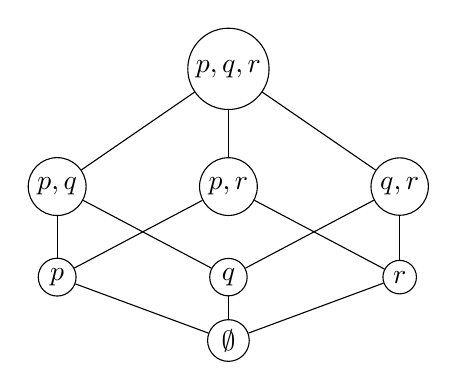
\begin{tikzpicture}[
        setnode/.style={draw,circle,inner sep=2pt},
        every edge/.style={draw},
        x=1.45cm,y=1.15cm
      ]
      \node[setnode] (empty) at (0,0) {\(\emptyset\)};

      \node[setnode] (p) at (-1.5,0.7) {\(\set{p}\)};
      \node[setnode] (q) at (0,0.7) {\(\set{q}\)};
      \node[setnode] (r) at (1.5,0.7) {\(\set{r}\)};

      \node[setnode] (pq) at (-1.5,1.7) {\(\set{p,q}\)};
      \node[setnode] (pr) at (0,1.7) {\(\set{p,r}\)};
      \node[setnode] (qr) at (1.5,1.7) {\(\set{q,r}\)};

      \node[setnode] (pqr) at (0,3) {\(\set{p,q,r}\)};

      \path
        (empty) edge (p)
        (empty) edge (q)
        (empty) edge (r)
        (p) edge (pq)
        (p) edge (pr)
        (q) edge (pq)
        (q) edge (qr)
        (r) edge (pr)
        (r) edge (qr)
        (pq) edge (pqr)
        (pr) edge (pqr)
        (qr) edge (pqr);
    \end{tikzpicture}
    \caption{Diagramma di Hasse del reticolo \(\langle 2^{\{p,q,r\}},\subseteq\rangle\).}
    \label{fig:ctl-power-set-lattice}
  \end{figure}

  Il nodo inferiore rappresenta \(\bot=\emptyset\), quello superiore rappresenta \(\top=W\). L'estremo superiore di due nodi è la loro unione, mentre l'estremo inferiore è la loro intersezione.
\end{example}

\begin{definition}{Funzioni monotone}
  Una funzione \(f: P \to P\) su un ordine parziale è \keyword{monotona} se \(\forall p_1, p_2 \in P\), \(p_1 \sqsubseteq p_2 \implies f(p_1) \sqsubseteq f(p_2)\); è \keyword{anti-monotona} se \(p_1 \sqsubseteq p_2 \implies f(p_2) \sqsubseteq f(p_1)\).
\end{definition}

\subsection{I teoremi di Tarski e Kleene}

\begin{theorem}{Tarski}
  Sia \(f: P \to P\) monotona su un ordine parziale completo. Allora il minimo punto fisso \(\mu x . f(x)\) e il massimo punto fisso \(\nu x . f(x)\) di \(f\) esistono, sono unici, e valgono:
  \[\mu x . f(x) = \bigsqcap \set{x\in P}[f(x) \sqsubseteq x] \qquad \nu x . f(x) = \bigsqcup \set{x\in P}[x \sqsubseteq f(x)]\]
\end{theorem}

Il teorema di Tarski garantisce esistenza e unicità, ma la caratterizzazione non è direttamente computazionale. Kleene fornì una caratterizzazione iterativa: definendo le iterate di \(f\) come
\[f^k(x) = \begin{cases}
    x             & ,k = 0 \\
    f(f^{k-1}(x)) & ,k > 0
  \end{cases}\]

\begin{theorem}{Kleene}
  Per \(f\) monotona e continua su un ordine parziale completo con minimo \(\bot\) e massimo \(\top\):
  \[\mu x . f(x) = \bigsqcup_{k\in\N} f^k(\bot) \qquad \nu x . f(x) = \bigsqcap_{k\in\N} f^k(\top)\]
\end{theorem}

Questa caratterizzazione è computazionalmente utile: se l'ordine ha catene finite (come \(2^W\) con \(W\) finito), l'iterazione si stabilizza in un numero finito di passi, e otteniamo un algoritmo generico:

\begin{algorithmdesc}{Calcolo del minimo punto fisso}
  \begin{algorithmic}[1]
    \Statex{} \textbf{signature} \(\textsc{LFP:} \quad \mathcal{P} \times \mathcal{P}^{\mathcal{P}} \to \mathcal{P} \)
    \Function{\(\textsc{LFP}\)}{$(P,\sqsubseteq,\bot,\top), f$} % chktex 46
    \State{} \(x_0 \gets \bot\)
    \State{} \(x_1 \gets f(x_0)\)
    \State{} \(j \gets 1\)
    \While{\(x_j \neq x_{j-1}\)}
    \State{} \(x_{j+1} \gets f(x_j)\) \Comment{\(x_j = f^j(\bot)\)}
    \State{} \(j \gets j + 1\)
    \EndWhile{}
    \State{} \Return{} \(x_j\)
    \EndFunction{}
  \end{algorithmic}
\end{algorithmdesc}

Per il massimo punto fisso (\textsc{GFP}) l'algoritmo è identico, con l'inizializzazione \(x_0 \gets \top\).

\section{Model checking di \(CTL\) come punto fisso}

Applichiamo ora la teoria al nostro contesto. Definiamo la \keyword{denotazione} di una formula \(\phi\) come l'insieme degli stati che la soddisfano:
\[\den{\phi}[][K] = \set{w \in W}[K,w\models \phi]\]

Si può notare che \(\phi_1 \to \phi_2 \implies \den{\phi_1} \subseteq \den{\phi_2}\). Astraendo il one-step unfolding di \(EU\) in una funzione su insiemi di stati:

\[f_U (V) = \den{\phi_2 \lor (\phi_1 \land EX\, V)} = \den{\phi_2} \cup \left(\den{\phi_1}\cap pre(V)\right) \]

dove \(pre(V) = \den{EX\, V}\) è la \keyword{preimmagine} di \(V\):
\[pre(V) = \set{w \in W}[\exists v \in V\st (w,v) \in R]\]

Dualmente per \(EG\):
\[f_G (V) = \den{\phi} \cap pre(V)\]

\begin{proposition}{Monotonia di \(pre\), \(f_U\) e \(f_G\)}
  \(V_1 \subseteq V_2 \implies pre(V_1)\subseteq pre(V_2)\), e di conseguenza \(f_U\) e \(f_G\) sono monotone su \(\langle 2^W, \subseteq\rangle\).
\end{proposition}
\begin{proof}
  Sia \(w \in pre(V_1)\): allora esiste \(v \in V_1\) con \((w,v) \in R\); ma \(V_1 \subseteq V_2\) implica \(v \in V_2\), e dunque \(w \in pre(V_2)\).
  Per \(f_U\) e \(f_G\): intersezioni e unioni con insiemi costanti rispetto a \(V\) preservano l'inclusione, poiché \(V_1 \subseteq V_2\) implica \(W'\cap V_1 \subseteq W'\cap V_2\) e \(W'\cup V_1 \subseteq W'\cup V_2\) per ogni \(W'\) costante.
\end{proof}

Per il teorema di Kleene possiamo dunque calcolare minimi e massimi punti fissi di \(f_U\) e \(f_G\). Resta da dimostrare che questi coincidano effettivamente con le denotazioni degli operatori \(CTL\)\@.

\begin{theorem}{Caratterizzazione a punto fisso di \(EU\) e \(EG\)}
  \[\den{E (\phi_1 U \phi_2)} = \mu V . f_U(V) \qquad \den{EG \phi} = \nu V . f_G(V)\]
\end{theorem}
\begin{proof}
  Dal one-step unfolding segue immediatamente che \(\den{E (\phi_1 U \phi_2)}\) e \(\den{EG\phi}\) sono punti fissi rispettivamente di \(f_U\) e \(f_G\): dunque \(\mu V . f_U(V)\subseteq \den{E (\phi_1 U \phi_2)}\) (il minimo punto fisso è incluso in ogni punto fisso) e \(\den{EG \phi} \subseteq \nu V. f_G(V)\) (Il massimo punto fisso include ogni punto fisso). Dobbiamo mostrare le inclusioni rimanenti.

  \begin{description}
    \item[\(\den{E (\phi_1 U \phi_2)} \subseteq \mu V . f_U(V)\).] 
    Essendo \(\mu V.f_U(V)\) un punto fisso, vale \(\den{\phi_2} \cup \left(\den{\phi_1}\cap pre(\mu V . f_U(V))\right) = \mu V . f_U(V)\), e in particolare \(\den{\phi_2} \subseteq \mu V . f_U(V)\).
    Procediamo per induzione sulla posizione \(i\) del primo punto che soddisfa \(\phi_2\) lungo un percorso testimone. Sia \(\hat{w} \in \den{E(\phi_1 U \phi_2)}\) e \(\hat{\pi} \in Path(K,\hat{w})\) un percorso con \(\hat\pi \models \phi_1 U \phi_2\) il cui primo punto che soddisfa \(\phi_2\) è \(i\).
    Per \(i = 0\), \(\hat{w} = {(\hat{\pi})}_0 \in \den{\phi_2} \subseteq \mu V . f_U(V)\).
    Per \(i > 0\), scriviamo \(\hat{\pi} = \hat{w}\, \pi\), dove \(\pi\) soddisfa \(\phi_1 U \phi_2\) con primo testimone in posizione \(i - 1\). Detto \(w = {(\pi)}_0\), per ipotesi induttiva \(w \in \mu V . f_U(V)\), e per definizione di \(pre\) si ha \(\hat{w} \in pre(\mu V . f_U(V))\). Inoltre \(\hat{w}\) non soddisfa \(\phi_2\) (per minimalità di \(i\)), dunque deve soddisfare \(\phi_1\), ovvero \(\hat{w}\in \den{\phi_1}\). Quindi
    \[\hat{w}\in \den{\phi_1}\cap pre(\mu V . f_U(V))\subseteq \den{\phi_2}\cup \left(\den{\phi_1}\cap pre(\mu V . f_U(V))\right) = \mu V . f_U(V)\]
    
    \item{\(\nu V . f_G(V) \subseteq \den{EG \phi}\).}
    Essendo \(\nu V . f_G(V)\) un punto fisso, vale \(\nu V . f_G(V) = \den{\phi} \cap pre(\nu V . f_G(V))\). Sia \(w \in \nu V . f_G(V)\): allora \(w \in \den{\phi}\) e \(w \in pre(\nu V . f_G(V))\), ovvero \(w\) ha almeno un successore ancora nel punto fisso. Iterando, da \(w\) si costruisce un percorso infinito che rimane dentro \(\nu V . f_G(V) \subseteq \den{\phi}\): tale percorso testimonia \(EG\phi\). Formalmente, supponendo per assurdo che ogni percorso da \(w\) raggiunga uno stato in cui \(\phi\) non è soddisfatta, per induzione sulla lunghezza del minimo prefisso che porta a tale stato si mostra che \(w \notin \nu V . f_G(V)\), assurdo.
  \end{description}
\end{proof}

\subsection{Algoritmi a punto fisso}

L'algoritmo per \(EU\) ed \(EG\) è dunque un'istanza di \textsc{LFP}/\textsc{GFP} con \(f = f_U\) (partendo da \(V_0 = \emptyset\)) o \(f = f_G\) (partendo da \(V_0 = W\)). Espandendo \(f_U\), la versione estesa per \(EU\) è:

\begin{algorithmdesc}{Compute \(EU\) come minimo punto fisso}
  \begin{algorithmic}[1]
    \Statex{} \textbf{signature} \(\textsc{ComputeEU:} \quad Kripke \times Formula \times Formula \to 2^W \)
    \Function{\(\textsc{ComputeEU}\)}{$(K, \phi_1, \phi_2)$} % chktex 46
    \State{} \(v_0 \gets \emptyset\) \Comment{\(\den{\bot}\)}
    \State{} \(v_1 \gets \den{\phi_2}\)
    \State{} \(j \gets 1\)
    \While{\(v_j \neq v_{j-1}\)}
    \State{} \(j \gets j + 1\)
    \State{} \(T \gets v_{j-1}\)
    \State{} \(V\gets \emptyset\)
    \While{\(T \neq \emptyset\)} \Comment{calcolo di \(pre(v_{j-1})\)}
    \State{} \(s \gets\) choose \(T\)
    \State{} \(T \gets T\setminus\set{s}\)
    \For{\(t \in R^{-1}(s)\)}
    \State{} \(V \gets V\cup\set{t}\)
    \EndFor{}
    \EndWhile{}
    \State{} \(v_{j} \gets \den{\phi_2} \cup \left(\den{\phi_1} \cap V\right)\)
    \EndWhile{}
    \State{} \textbf{return} \(v_j\)
    \EndFunction{}
  \end{algorithmic}
\end{algorithmdesc}

\begin{note}{}
  La formulazione a punto fisso può sembrare solo una rilettura elegante degli algoritmi di etichettatura, ma è molto di più: il calcolo iterato di \(pre\), unioni e intersezioni su insiemi di stati è esattamente ciò che sapremo implementare in modo \emph{simbolico} tramite OBDD, senza mai enumerare esplicitamente gli stati. Questo sarà l'argomento del prossimo capitolo.
\end{note}

\section{Model checking di \texorpdfstring{\(CTL^*\)}{CTL*}}

Torniamo ora alla logica completa \(CTL^*\) e vediamo come risolverne il model checking combinando le tecniche di LTL e \(CTL\)\@.

Consideriamo la proprietà \(E F(p\land X q)\): non è una formula \(CTL\) (l'operatore \(X\) non è preceduto da un quantificatore), ma è della forma \(Q\, \psi\) con \(Q\) quantificatore e \(\psi\) formula LTL\@. In questi casi bastano gli strumenti della~\Cref{sec:buchi}: per \(E\psi\) è sufficiente intersecare l'automa della struttura di Kripke con \(A_\psi\) e verificare che il linguaggio sia non vuoto; per \(A\psi\), dualmente, si verifica che l'intersezione con \(A_{\neg\psi}\) sia vuota:
\[K,w\models Q\psi \iff \begin{cases}
    \mathcal{L}(A_{\psi} \Cap A_{K,w}) \neq \emptyset       & ,Q = E \\
    \mathcal{L}(A_{\neg \psi} \Cap A_{K,w}) = \emptyset & ,Q = A
  \end{cases}\]

Consideriamo però \(E(X (E \psi) \land G (A \psi'))\), che non è né LTL quantificata né \(CTL\)\@. L'idea dell'etichettatura bottom-up torna utile: da grammatica, i casi base di ogni formula \(CTL^*\) sono formule LTL quantificate, che sappiamo risolvere. Una volta etichettati gli stati con una sottoformula quantificata \(Q\psi\), possiamo considerarla come una \emph{nuova proposizione atomica} \(p_{Q\psi}\), sostituirla nella formula esterna, e procedere ricorsivamente: a ogni passo la formula più interna torna a essere della forma \(Q\, \psi_{LTL}\), riapplicando il caso base.

\begin{example}{}
  Prendiamo \(\phi \equiv EX(EG(EFp)) \land G(AF(p\land X(EXq)))\). L'albero di dipendenze tra sottoformule quantificate, derivato dall'albero sintattico, è:

  \begin{center}
    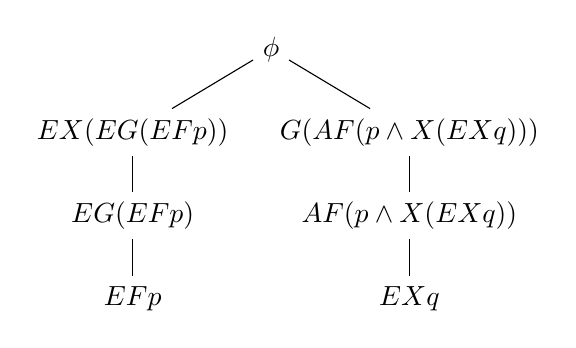
\begin{tikzpicture}[sibling distance=10em, level distance=3em]
      \node {\(\phi\)}
      child { node {\(EX(EG(EFp))\)}
          child { node {\(EG(EFp)\)}
              child { node {\(EFp\)}}
            }
        }
      child { node {\(G(AF(p\land X(EXq)))\)}
          child { node {\(AF(p\land X(EXq))\)}
              child { node {\(EXq\)}}
            }
        };
    \end{tikzpicture}
  \end{center}

  Il flattening con le proposizioni atomiche fresche procede dalle foglie verso la radice:

  \begin{center}
    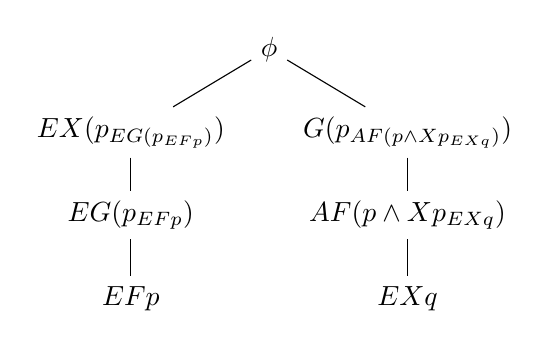
\begin{tikzpicture}[sibling distance=10em, level distance=3em]
      \node {\(\phi\)}
      child { node {\(EX(p_{EG(p_{EFp})})\)}
          child { node {\(EG(p_{EFp})\)}
              child { node {\(EFp\)}}
            }
        }
      child { node {\(G(p_{AF(p\land X p_{EXq})})\)}
          child { node {\(AF(p\land X p_{EXq})\)}
              child { node {\(EXq\)}}
            }
        };
    \end{tikzpicture}
  \end{center}
\end{example}

La complessità di questo algoritmo è \(n\) volte quella del model checking LTL (PSPACE), con \(n\) numero di sottoformule quantificate, lineare nella lunghezza della formula: la complessità totale resta dunque PSPACE\@. Un approccio alternativo usa gli automi ad albero, ottenendo anch'esso PSPACE\@. Per soddisfacibilità e validità, invece, si può mostrare che \(CTL^*\) arriva a 2EXPTIME, a differenza di LTL che rimane PSPACE\@.

\section{Espressività a confronto: LTL, \(CTL\) e \texorpdfstring{\(CTL^*\)}{CTL*}}

\(CTL^*\) offre un notevole guadagno di espressività. LTL è contenuta in \(CTL^*\), poiché ogni formula \(\psi \in LTL\) equivale ad \(A \psi\) in \(CTL^*\). È interessante anche il problema inverso: data \(\phi \in CTL^*\), esiste \(\psi \in LTL\) tale che \(\phi \equiv A\psi\)?

È stato dimostrato che, presa una formula in \(CTL^*\) ed eliminando semplicemente tutti i quantificatori di percorso, si ottiene una formula LTL che è \emph{l'unica candidata possibile}: se esiste una formula LTL equivalente all'originale (una volta quantificata universalmente), è quella. Di conseguenza, data \(\phi \in CTL^*\), si produce \(\hat{\phi} \in LTL\) eliminando i quantificatori e si verifica se \(\phi \equiv A \hat{\phi}\), riducendo il problema alla soddisfacibilità della formula \(\neg ((\phi \to A \hat{\phi}) \land (A\hat{\phi} \to \phi))\): se è soddisfacibile le formule non sono equivalenti, altrimenti lo sono. Essendo \(CTL\) un frammento di \(CTL^*\), lo stesso procedimento si applica anche a formule \(CTL\)\@.

La domanda inversa, ovvero se data \(\psi \in LTL\) esista \(\phi \in CTL\) tale che \(A\psi \equiv \phi\), è invece decidibile caso per caso ma la caratterizzazione generale è a oggi un problema aperto.

\subsection{Formule \texorpdfstring{\(CTL^*\)}{CTL*} non esprimibili in \(CTL\)}

\begin{example}{\(A FGp\)}
  Consideriamo il modello con tre stati: uno stato \(p\) con self-loop, da cui si passa a uno stato \(\neg p\), da cui si passa a un secondo stato \(p\) con self-loop.
  La struttura e la sua estensione ad albero sono mostrate in figura. Nel modello, il primo stato \(p\) ha due possibilità: rimanere in sé stesso oppure passare allo stato \(\neg p\). Dallo stato \(\neg p\) si raggiunge necessariamente il secondo stato \(p\), che ha poi un self-loop.

  \begin{figure}[H]
    \centering
    \begin{tikzpicture}[shorten >=1pt,node distance=1.35cm,on grid,auto,font=\small]
      
      \node[state] (af_s0) {\(s_0\)};
      \node[state] (af_s1) [right=of af_s0] {\(s_1\)};
      \node[state] (af_s2) [right=of af_s1] {\(s_2\)};
      \path[->]
        (af_s0) edge [loop above] ( )
        (af_s0) edge (af_s1)
        (af_s1) edge (af_s2)
        (af_s2) edge [loop above] ( );
      \node[below=0.3cm of af_s0] {\(p\)};
      \node[below=0.3cm of af_s1] {\(\neg p\)};
      \node[below=0.3cm of af_s2] {\(p\)};
            \end{tikzpicture}
    \caption{Il modello per \(A FGp\)}\label{fig:ctl-afgp-model}
  \end{figure}

  In questo modello vale \(A FGp\): ogni percorso da un certo punto in poi rimane per sempre in uno stato \(p\). Proviamo a tradurla in \(CTL\)\@. Le candidate più ovvie sono \(AF(AGp)\) e \(AF(EGp)\). La prima è già falsa nel modello di esempio: nel percorso che rimane per sempre nel primo stato \(p\), nessuno stato soddisfa \(AGp\), perché da ogni prefisso è sempre possibile deviare verso \(\neg p\). La seconda è vera nel modello dato, ma esistono altri modelli in cui \(AFGp\) è vera e \(AF(EGp)\) no, poiché la prima formula richiede che ogni percorso \textit{prima o poi} soddisfi \textit{sempre} \(p\), mentre la seconda richiede che ogni percorso \textit{prima o poi} abbia un \textit{sottopercorso} in cui \(p\) è sempre vero. Una possibile lettura del problema è che la natura esistenziale del testimone di \(F\) mal si combina con la quantificazione universale esterna.
\newline
  Consideriamo ora la formula \(AF(p \land Xp)\).
  La candidata ovvia \(AF(p \land AXp)\) è falsa già nel modello dell'esempio precedente: nel percorso di soli \(p\), ogni stato ha almeno un successore etichettato \(\neg p\), mentre \(AF(p \land Xp)\) è vera. Considerando invece \(AF (p\land EXp)\), questa è soddisfatta dal modello seguente:

  \begin{figure}[H]
    \centering
    \begin{tikzpicture}[shorten >=1pt,node distance=1.35cm,on grid,auto,font=\small]
      
      \node[state] (af_s0) {\(s_0\)};
      \node[state] (af_s1) [right=of af_s0] {\(s_1\)};
      \node[state] (af_s2) [right=of af_s1] {\(s_2\)};
      \path[->]
        (af_s1) edge [loop above] ( )
        (af_s0) edge (af_s1)
        (af_s1) edge (af_s2)
        (af_s2) edge [loop above] ( );
      \node[below=0.3cm of af_s0] {\(\neg p\)};
      \node[below=0.3cm of af_s1] {\(p\)};
      \node[below=0.3cm of af_s2] {\(\neg p\)};
            \end{tikzpicture}
    \caption{Il modello per \(A FGp\)}\label{fig:ctl-afgp-model-2}
  \end{figure}
   
   la cui estensione ad albero contiene percorsi in cui non ci sono mai due \(p\) consecutive: la formula originale non è soddisfatta, e dunque le due non sono equivalenti.
\newline
  Infine, considerando una tipica formula per esprimere la Fairness: \(A(GFp\to Fq)\).
  La candidata \(AG(AF p) \to AFq\) sposta lo scope del quantificatore iniziale: modelli che falsificherebbero l'originale possono soddisfare la seconda semplicemente falsificando la premessa dell'implicazione. Le proprietà di fairness sono l'esempio classico di formule \(CTL^*\)/LTL non esprimibili in \(CTL\)\@.
\end{example}

\subsection{Formule \(CTL\) non esprimibili in LTL}

\begin{example}{\(AG(EFp)\)}
  Vogliamo mostrare che non esiste \(\psi \in LTL\) tale che \(AG(EFp) \equiv A\psi\). Supponiamo per assurdo che esista.

  Consideriamo il modello \(K\) mostrato in figura.

  \begin{figure}[H]
    \centering
    \begin{tikzpicture}[shorten >=1pt,node distance=1.55cm,on grid,auto,font=\small]
      \node[state] (ag_s0) {\(s_0\)};
      \node[state] (ag_s1) [right=of ag_s0] {\(s_1\)};
      \node[state] (ag_s2) [above right=of ag_s1] {\(s_2\)};
      \node[state] (ag_s3) [below right=of ag_s1] {\(s_3\)};
      \path[->]
        (ag_s0) edge (ag_s1)
        (ag_s1) edge (ag_s2)
        (ag_s1) edge (ag_s3)
        (ag_s2) edge [loop above] ()
        (ag_s3) edge [loop below] ();
      \node[below=0.3cm of ag_s0] {\(\neg p\)};
      \node[below=0.3cm of ag_s1] {\(\neg p\)};
      \node[below=0.3cm of ag_s2] {\(\neg p\)};
      \node[below=0.3cm of ag_s3] {\(p\)};
    \end{tikzpicture}
    \caption{Il modello \(K\) per la dimostrazione di \(AG(EFp)\).}\label{fig:ctl-agefp-model}
  \end{figure}
   
   Poiché \(s_3\) è raggiungibile da \(s_0\), \(K \models AG(EFp)\), e dunque \(K \models A\psi\).

  Consideriamo ora il modello \(K'\) ottenuto rimuovendo \(s_3\): qui \(p\) non è mai soddisfatta, dunque \(K' \not\models AG(EFp)\). Ma tutti i percorsi infiniti di \(K'\) sono anche percorsi di \(K\): essendo che le formule LTL sono valutate sui percorsi, da \(K \models A\psi\) segue \(K' \models A\psi\), e quindi \(K' \models AG(EFp)\), assurdo.
\end{example}

\subsection{La gerarchia di espressività}

Riassumendo, LTL (intesa come frammento delle \(A\psi\)) e \(CTL\) sono incomparabili, entrambe strettamente contenute in \(CTL^*\):
\begin{itemize}
  \item \(A (p U q)\) appartiene all'intersezione di LTL e \(CTL\);
  \item \(AG(EFp)\) è esprimibile solo in \(CTL\);
  \item \(AF(p \land Xp)\) e \(A(GFp \to Fq)\) sono esprimibili solo in LTL;
  \item la congiunzione di una formula solo-CTL e una solo-LTL è esprimibile solo in \(CTL^*\).
\end{itemize}
\begin{figure}[H]
  \centering
  \begin{tikzpicture}[
      set/.style={draw, thick, ellipse, minimum width=5.3cm, minimum height=3.9cm,
        align=center},
      example/.style={font=\scriptsize, align=center}
    ]
    \node[draw, thick, fill=none, minimum width=14cm, minimum height=8cm,
      rounded corners=2pt] (frame) {};
    \node[set, fill=green!18, minimum width=11.2cm, minimum height=6.5cm] (ctls) {};
    \node[above=0.1cm of ctls.north, text=green!50!black] {\(CTL^*\)};
    \node[set, fill=blue!18, fill opacity=0.72, text opacity=1,
      xshift=-1.45cm] (ltl) {};
    \node[above=0.1cm of ltl.north, text=blue!60!black] {\(LTL\)};
    \node[set, fill=orange!25, fill opacity=0.72, text opacity=1,
      xshift=1.45cm] (ctl) {};
    \node[above=0.1cm of ctl.north, text=orange!80!black] {\(CTL\)};

    \node[example, below left=0.25cm and 0.05cm of ltl.center]
      {$A(GFp\to Fq)$};
    \node[example, below right=0.25cm and 0.05cm of ctl.center]
      {$AG(EFp)$};
    \node[example, above=2.5cm of ctls.south]
      {$A(p\,U\,q)$};
    \node[example, below=0.25cm of ctls.south]
      {CTL e LTL incomparabili};
  \end{tikzpicture}
  \caption{Gerarchia di espressività tra LTL, CTL e \(CTL^*\).}\label{fig:ctl-expressiveness-hierarchy}
\end{figure}

\chapter{Giochi e Logiche per Strategie}\label{ch:atl}

Le strutture di Kripke modellano tutto ciò che non è il sistema come un'unica entità inglobata dal non determinismo. In molti contesti, però, il sistema evolve per effetto di più \emph{agenti} che interagiscono, con obiettivi antagonisti, collaborativi o misti: processi in un sistema distribuito, robot in un ambiente condiviso, o letteralmente giocatori in un gioco. In questo capitolo introduciamo le \keyword{concurrent game structure} per modellare queste interazioni, e la logica \keyword{ATL} (\textit{Alternating-time Temporal Logic}), un'estensione di CTL per parlare di \emph{strategie}.

\section{Concurrent Game Structures}

\begin{definition}{Concurrent Game Structure}
  Una \keyword{concurrent game structure} è una tupla \(G=\langle AP, Ag, Ac, Ps, p_0, \delta, \lambda \rangle\) con:
  \begin{itemize}
    \item \(AP\) insieme di proposizioni atomiche
    \item \(Ag\) insieme di agenti o giocatori
    \item \(Ac\) insieme di azioni che gli agenti possono compiere\footnote{È possibile anche avere un insieme di azioni per ogni agente, ma per semplicità consideriamo un unico insieme condiviso.}
    \item \(Ps\) insieme delle \keyword{posizioni} del gioco, analoghe agli stati di una struttura di Kripke
    \item \(p_0 \in Ps\) posizione iniziale
    \item \(\delta: Ps \times Ac^{Ag} \to Ps\) funzione di transizione
    \item \(\lambda: Ps \to 2^{AP}\) funzione di etichettatura
  \end{itemize}
\end{definition}

La struttura è molto vicina a una struttura di Kripke \(K=\langle AP,W,w_0,R,\lambda\rangle\). La differenza principale è che \(\delta\) non è una relazione ma una \emph{funzione}: l'evoluzione è deterministica \emph{a valle delle azioni degli agenti}. Stiamo modellando giochi concorrenti (non a turni): \(Ac^{Ag}\) è l'insieme delle funzioni che associano a ogni agente un'azione, ed è questo insieme a catturare il non determinismo, che nelle strutture di Kripke era anonimo e qui è invece attribuito alle scelte dei giocatori.

\begin{note}{}
  Rappresentando gli agenti con numeri, una funzione \(d \in Ac^{Ag}\) si può esprimere come tupla in cui la posizione \(i\)-esima è l'azione dell'agente \(i\): ad esempio \(\delta(p,(S,C))\) equivale a \(\delta(p, d)\) con \(d(1) = S\) e \(d(2) = C\). Tali funzioni sono dette \keyword{decisioni collettive}.
\end{note}

\begin{example}{Sasso-carta-forbice}
  Modelliamo sasso-carta-forbice come gioco giocato una sola volta:
  \begin{itemize}
    \item \(Ag = \set{1,2}\)
    \item \(Ac = \set{S,C,F}\)
    \item \(Ps = \set{p_0, p_1, p_2}\), con \(p_0\) posizione iniziale senza vincitore, \(p_1\) vittoria del giocatore 1 e \(p_2\) vittoria del giocatore 2
  \end{itemize}
  La funzione di transizione è:
  \[\delta(p,(a_1,a_2)) = \begin{cases}
      p_0 & \text{se } a_1 = a_2 \land p = p_0                                 \\
      p_1 & \text{se } (a_1,a_2) \in \set{(S,F),(C,S),(F,C)} \land p = p_0     \\
      p_2 & \text{se } (a_1,a_2) \in \set{(S,C),(C,F),(F,S)} \land p = p_0     \\
      p   & \text{se } p \in \set{p_1,p_2}
    \end{cases}\]
  Le posizioni di vittoria sono assorbenti perché il gioco si gioca una volta sola. Per verificare proprietà sulla vittoria si può prendere \(AP = \set{{win}_1, {win}_2}\), con \(\lambda(p_0) = \emptyset\), \(\lambda(p_1) = \set{{win}_1}\) e \(\lambda(p_2) = \set{{win}_2}\).
  \begin{figure}[H]
    \centering
    \begin{tikzpicture}[
        node distance=3.2cm,
        >=Stealth,
        every node/.style={font=\small},
        state/.style={circle, draw, thick, minimum size=1.1cm, align=center},
        outcome/.style={state, minimum size=1.35cm},
        transition/.style={->, thick}
      ]
      \node[state] (rps_p0) {\(p_0\)};
      \node[outcome, right=of rps_p0, yshift=1.65cm] (rps_p1)
        {\(p_1\)};
      \node[outcome, right=of rps_p0, yshift=-1.65cm] (rps_p2)
        {\(p_2\)};

      \path[transition]
        (rps_p0) edge[loop above] node[align=center]
          {\((A,A), A\in Ac\)} ()
        (rps_p0) edge[bend left=12] node[above, align=center]
          {\(\substack{(S,F)\\(C,S)\\(F,C)}\)} (rps_p1)
        (rps_p0) edge[bend right=12] node[below, align=center]
          {\(\substack{(S,C)\\(C,F)\\(F,S)}\)} (rps_p2)
        (rps_p1) edge[loop above] node {\(\forall d\in Ac^{Ag}\)} ()
        (rps_p2) edge[loop below] node {\(\forall d\in Ac^{Ag}\)} ();

      \node[right=0.15cm of rps_p1] {vittoria del giocatore 1};
      \node[right=0.15cm of rps_p2] {vittoria del giocatore 2};
      \node[left=0.55cm of rps_p0] {pareggio};
    \end{tikzpicture}
    \caption{Automa delle transizioni per il gioco del sasso-carta-forbice.}\label{fig:atl-rock-paper-scissors}
  \end{figure}
\end{example}

La modellazione è sufficientemente generale da catturare anche giochi \emph{a turni}, semplicemente ignorando nella funzione di transizione le azioni dei giocatori di cui non è il turno.

\begin{example}{Tris}
  Per il tris abbiamo \(Ag = \set{\times, \circ}\) e possiamo codificare le caselle (e dunque le azioni, essendo che ogni giocatore può solo riempire una casella col proprio simbolo) con i numeri da \(1\) a \(9\). Enumerare esplicitamente gli stati è impraticabile: il modo migliore è descrivere le posizioni come funzioni \(\set{1,\ldots,9} \to \set{\square, \times, \circ}\) che associano a ogni cella il suo contenuto (vuota, croce, cerchio), più due posizioni \(\bot_{\times}, \bot_{\circ}\) per le mosse non valide, modellate come sconfitta automatica di chi le compie.

  La posizione iniziale è la funzione costante \(p_0: n \mapsto \square\). La codifica del turno avviene nella funzione di transizione, che ignora l'azione del giocatore a cui non tocca: ad esempio, per la prima mossa (turno di \(\times\)),
  \[\delta(p_0, d) = p_i \quad\text{con }\quad i = d(\times), p_i: \begin{cases}
    i \mapsto \times,\\
    n \mapsto \square\quad\forall n\neq i
  \end{cases}\]
  e per la risposta di \(\circ\) alla mossa in cella 5:
  \[\delta(p_5, d) = p_{5i} \quad\text{con } i = d(\circ), p_{5i}: \begin{cases}
    5 \mapsto \times,\\
    i \mapsto \circ,\\
    n \mapsto \square\quad\forall n\notin \set{i,5}
  \end{cases}\]
  \begin{figure}[H]
    \centering
    \includegraphics[width=\textwidth]{_images/Tris_states}
    \caption{Grafo degli stati del tris. I numeri  la quantità di posizioni simmetricamente equivalenti.}\label{fig:atl-tic-tac-toe-states}
  \end{figure}
\end{example}

\section{Strategie, storie e play}

Ci serve ora un linguaggio per esprimere proprietà di questi sistemi. Prima però formalizziamo i concetti di percorso e strategia.

\begin{definition}{Percorsi e storie}
  Diremo che \(\pi \in {Ps}^\omega\) è un \keyword{percorso} della struttura di gioco \(G\) (denotato \(\pi \in Path(G)\)) se per ogni \(i\in\N\) esiste \(d \in Ac^{Ag}\) tale che \(\pi_{i+1} = \delta(\pi_i,d)\).\footnote{ è equivalente a vedere i percorsi nella struttura di Kripke sottostante.}
  
  Una \keyword{storia} è un sottopercorso finito, l'insieme delle storie è denotato \(Hst\):
  \[Hst = \set{\pi \in Path(G)}[\abs{\pi} < \omega]\]
\end{definition}

\begin{definition}{Strategie}
  Una \keyword{strategia} per un agente è una funzione
  \[\sigma: Hst \to Ac\]
  che associa a ogni storia l'azione da compiere.
  
  Una strategia per una coalizione \(A\subseteq Ag\) è una famiglia \(\sigma_A = \set{\sigma_a}_{a \in A}\) di strategie, una per ogni agente della coalizione.
\end{definition}

Le strategie dipendono in generale dall'intera storia, non solo dall'ultima posizione. Questo fenomeno esisteva già nelle strutture di Kripke e nelle logiche temporali: la struttura in \Cref{fig:kripke-history} verifica \(F(p\land Fq)\), ma per testimoniarlo è necessario fare scelte \emph{diverse} nello stesso stato \(w_0\) in momenti diversi, ricordando le scelte passate. Con scelte basate solo sullo stato corrente si possono realizzare solo percorsi a \keyword{lasso} (un prefisso seguito da un ciclo ripetuto per sempre).

\begin{figure}[H]
    \begin{minipage}{0.48\textwidth}
      \centering
      \includegraphics[width=\linewidth]{_images/kripke_history}
      \caption{Struttra di Kripke con memoria.}\label{fig:kripke-history}
    \end{minipage}
    \hfill
    \begin{minipage}{0.48\textwidth}
      \centering
      \includegraphics[width=\linewidth]{_images/kripke_lasso}
      \caption{Struttra di Kripke a lasso.}\label{fig:kripke-lasso}
    \end{minipage}
  \end{figure}


Si dimostra però che la memoria è indispensabile solo per proprietà con operatori temporali \emph{annidati}: rimanendo in CTL, o come vedremo in ATL, la memoria non è necessaria.

\begin{definition}{Play}
  Una coppia di strategie di due coalizioni complementari (\(A\) e \(Ag\setminus A\)) identifica un unico percorso, detto \keyword{play}:
  \[\pi = play(\sigma_A,\sigma_{Ag\setminus A}, p_0) \in Path(G,p_0)\]
  definito da \(\pi_{i+1} = \delta(\pi_i, d_i)\) per ogni \(i \in \N\), con
  \[d_i(a) = \begin{cases}
      \sigma_A^a(\pi_{\leq i})            & a \in A            \\
      \sigma_{Ag\setminus A}^a(\pi_{\leq i}) & a \in Ag\setminus A
    \end{cases}\]
  ovvero a ogni passo la posizione successiva è determinata dalle azioni scelte dalle strategie, che dipendono dalla storia fino a quel punto.
\end{definition}

\section{\texorpdfstring{\(ATL\)}{ATL} e \texorpdfstring{\(ATL^*\)}{ATL*}}

Le logiche \(ATL\) e \(ATL^*\) estendono CTL e \(CTL^*\) sostituendo i quantificatori di percorso con \keyword{quantificatori strategici} sulle coalizioni. Il nome \textit{alternating} viene dalle macchine alternanti: a differenza delle macchine non deterministiche (esistenziali) o universali, qui si ha un'\emph{alternanza} di esistenzialità e universalità.

\begin{definition}{Grammatica di \(ATL^*\)}
  \[\phi ::= p \mid \neg \phi \mid \phi \land \phi \mid \phi \lor \phi \mid \GDia[A]\psi \mid \GBox[A] \psi\]
  \[\psi ::= \phi \mid \neg \psi \mid \psi \land \psi \mid \psi \lor \psi \mid X\psi \mid \psi U\psi \mid \psi R \psi\]
  con \(A \subseteq Ag\) coalizione. \(ATL\) è il frammento in cui, come in CTL, ogni operatore temporale è immediatamente preceduto da un quantificatore strategico:
  \[\psi ::= X\phi \mid \phi U\phi \mid \phi R \phi\]
  
  La semantica dei quantificatori strategici in \(ATL\), data una struttura di Kripke \(G\) e uno stato \(p\), è:
  \[G,p\models \GDia[A] \psi \text{ se } \exists \sigma_A \in Str(A)\ \forall \sigma_{\overline{A}} \in Str(\overline{A}).\ G,play(\sigma_A,\sigma_{\overline{A}},p)\models \psi \]
  \[G,p\models \GBox[A] \psi \text{ se } \forall \sigma_A \in Str(A)\ \exists \sigma_{\overline{A}} \in Str(\overline{A}).\ G,play(\sigma_A,\sigma_{\overline{A}},p)\models \psi \]
\end{definition}
Intuitivamente:
\begin{itemize}
\item \(\GDia[A] \psi\) è vera se \emph{esiste} una strategia \(\sigma_A\) per la coalizione \(A\) tale che, \emph{per ogni} strategia \(\sigma_{\overline{A}}\) della coalizione complementare \(\overline{A} = Ag\setminus A\), il play risultante soddisfa \(\psi\): la coalizione \(A\) può \emph{garantire} \(\psi\);
\item \(\GBox[A] \psi\) è vera se \emph{per ogni} strategia \(\sigma_A\) di \(A\) \emph{esiste} una strategia \(\sigma_{\overline{A}}\) di \(\overline{A}\) tale che il play soddisfa \(\psi\): la coalizione \(A\) non può \emph{evitare} \(\psi\).
\end{itemize}

I due operatori sono duali, dalla dualità semantica dei quantificatori: \(\neg \GDia[A]\psi \equiv \GBox[A] \neg \psi\).

\subsection{Relazione con CTL}

La struttura di Kripke indotta da una concurrent game structure ha \(R\) tale che \((s_1,s_2) \in R\) se e solo se \(\exists d \in Ac^{Ag}.\ s_2 = \delta(s_1,d)\). Questo giustifica il vedere ATL come estensione di CTL, e in particolare \(\GDia\) e \(\GBox\) come generalizzazioni di \(E\) e \(A\):

\begin{proposition}{}
  \(\GDia[Ag] \psi\equiv E\psi\) e \(\GBox[Ag] \psi \equiv A\psi\), dove \(Ag\) è la \keyword{grand coalition} di tutti gli agenti.
\end{proposition}
\begin{proof}
  \begin{description}
    \item[{\(\GDia[Ag] \psi \equiv E\psi\):}] Si ha che \(\GDia[Ag] \psi\) è vera se \(\exists \sigma_{Ag} \forall \sigma_{\emptyset}.G,play(\sigma_{Ag},\sigma_{\emptyset},s)\models \psi\). Di conseguenza la quantificazione universale è vacua, e quindi \(\GDia[Ag] \psi\) se e solo se \(\exists \sigma_{Ag}.G,play(\sigma_{Ag},\sigma_{\emptyset},s)\models \psi\). Essendoci però un unica coalizione, la strategia \(\sigma_{Ag}\) determina un unico play, e quindi da sola definisce un unico percorso \(\pi\) che soddisfa \(\psi\). Dunque \(\GDia[Ag] \psi\) se e solo se \(E\psi\).
    
    \item[{\(\GBox[Ag] \psi \equiv A\psi\):}] Si dimostra similmente.
  \end{description}
\end{proof}

CTL è dunque semanticamente il frammento di ATL in cui si scelgono solo le coalizioni \(A=\emptyset\) o \(A = Ag\), rendendo vacuo uno dei due quantificatori. ATL è strettamente più espressiva: gli operatori \(\GDia\) e \(\GBox\) nascondono una quantificazione \emph{alternata} (\(\exists\forall\), \(\forall\exists\)) che CTL non può esprimere.

\begin{example}{Strategie in sasso-carta-forbice}
  Nel gioco del sasso-carta-forbice esistono \q{weak strategy}: per ogni agente c'è una strategia dell'avversario che lo fa vincere,
  \[\GBox[\set{1}] F\, s_1\land \GBox[\set{2}] F\, s_2\]
  ma non esistono strategie vincenti garantite:
  \[\neg \GDia[\set{1}] F\, s_1 \land \neg \GDia[\set{2}] F\, s_2\]
\end{example}

\subsection{Strategie memoryless}

Ci concentreremo su ATL (non \(ATL^*\)) perché gode di una proprietà fondamentale: può essere soddisfatta da strategie \keyword{memoryless}, ovvero funzioni \(\sigma: Ps\to Ac\) in cui conta solo l'ultima posizione. Non vedremo la dimostrazione, ma l'idea è che, come per CTL, le proprietà che richiedono memoria richiedono nesting di operatori temporali, assente in ATL: se una formula è soddisfatta da percorsi con cicli non semplici, si possono sempre accorpare i cicli ottenendo la struttura a lasso.

Le strategie memoryless di fatto selezionano archi: un play identifica un \emph{sottografo} in cui si mantengono solo gli archi effettivamente percorribili. Tale sottografo è oltretutto deterministico (dalla posizione iniziale esiste un solo percorso), e la verifica di proprietà si riduce a raggiungibilità sui sottografi indotti.

\section{Model checking di ATL}

Per il model checking di CTL abbiamo sfruttato il one-step unfolding, che ci ha permesso di costruire funzioni monotone e usare i punti fissi. Facciamo lo stesso per ATL\@. Vogliamo mostrare:
\[\GDia[A] (\phi_1 U\phi_2) \equiv \phi_2 \lor (\phi_1\land \GDia[A] X\, \GDia[A] (\phi_1 U\phi_2))\]

È facile vedere che \(\GDia[A] (\phi_1 U\phi_2) \equiv \phi_2 \lor (\phi_1\land \GDia[A] X (\phi_1 U\phi_2))\): basta usare la stessa strategia. La parte delicata è \emph{spezzare} l'operatore temporale inserendo il secondo \(\GDia[A]\). In CTL spezzare un percorso era immediato: il next è la testa, l'until il resto. Qui invece c'è un'alternanza di quantificatori: a sinistra una singola strategia scelta a priori garantisce l'intero until, a destra abbiamo una \emph{doppia} alternanza:
\[\exists \sigma_A \forall \sigma_{\overline{A}}\ \exists \sigma_{A}' \forall \sigma_{\overline{A}}'.\ play\left(\sigma_{A}',\sigma_{\overline{A}}',{\left(play(\sigma_A,\sigma_{\overline{A}},s)\right)}_1\right) \models \phi_1 U \phi_2\]

Quello che vogliamo mostrare è che questa doppia alternanza è irrilevante, e che bastano i primi due quantificatori. Ci sono due strade.

La prima passa per il teorema di Zermelo: per i giochi a turni, finiti e a somma zero, il cui goal è un'istanza di reachability, almeno un giocatore ha una strategia vincente:
\[\exists \sigma_1 \forall \sigma_2.\ Win_1(\sigma_1,\sigma_2)\ \lor\ \exists \sigma_2 \forall \sigma_1.\ Win_2(\sigma_1,\sigma_2) \]
Si noti che al prim'ordine questa struttura è falsificabile (basta un modello a grafo senza elementi minimi né massimi), ma per i giochi finiti a somma zero è sempre verificata. Si costruisce quindi un gioco a somma zero tra un \emph{verificatore} e un \emph{falsificatore} della formula e si sfrutta Zermelo per mostrare che uno dei due ha una strategia vincente.

La seconda strada è costruttiva: si usano le strategie della formula assunta vera per costruire quelle della formula da mostrare equivalente. Per \(\GDia[A] X (\phi_1 U\phi_2) \implies \GDia[A] X\, \GDia[A] (\phi_1 U\phi_2)\) si copia la strategia; nell'altro verso se ne hanno due, quella del next e quella dell'until: si usa la prima per il primo passo, e poi la seconda \emph{dimenticando} il primo stato dalla storia. Si passa temporaneamente per strategie con memoria, che si possono però sempre riportare a memoria zero.

Lo stesso vale per il release:
\[\GDia[A] (\phi_1 R \phi_2) \equiv \phi_2 \land (\phi_1 \lor \GDia[A] X\, \GDia[A] (\phi_1 R\phi_2))\]

\begin{warning}{}
  A differenza di CTL, non è possibile ridurre il release a \(G\), perché il quantificatore strategico \emph{non distribuisce} sulla disgiunzione:
  \[\GDia[A] (\phi_1 R \phi_2) \equiv \GDia[A] \left((\phi_2 U (\phi_1 \land \phi_2)) \lor G \phi_2\right) \not\equiv \GDia[A] (\phi_2 U (\phi_1 \land \phi_2)) \lor \GDia[A] G \phi_2\]
  La strategia che garantisce la disgiunzione può realizzare disgiunti diversi contro avversari diversi, senza garantirne nessuno singolarmente.
\end{warning}

Con la stessa identica dimostrazione vista per CTL, queste equazioni caratterizzano rispettivamente minimo e massimo punto fisso; l'unica differenza è che l'induzione è completa su un albero di percorsi, piuttosto che lineare su un singolo percorso.

\subsection{La preimmagine alternante}

Ciò che resta da adattare è l'operatore \(X\), ovvero, in forma denotazionale, la funzione \(pre\). Questa è la vera differenza sostanziale: con più giocatori il concetto di preimmagine è più fine. Prima \(pre\) catturava \(EX\); ora dobbiamo catturare \(\GDia[A]X\). Lavorando su un solo passo, delle strategie interessa solo l'azione nella posizione corrente:
\[\exists \sigma_A \forall \sigma_{\overline{A}}.\ play(\sigma_A,\sigma_{\overline{A}},s) \models X\phi
  \quad\text{diventa}\quad
  \exists {ac}_{A} \forall {ac}_{\overline{A}}.\ \delta(s, ({ac}_A, {ac}_{\overline{A}})) \models \phi\]

La definizione di \(pre\) va dunque aggiornata per trattare l'universale interno:
\[pre_A(V) = \set{s\in Ps}[\exists {ac}_{A} \in Ac^A\ \forall {ac}_{\overline{A}} \in Ac^{\overline{A}}.\ \delta(s, ({ac}_A, {ac}_{\overline{A}})) \in V]\]

A livello algoritmico, l'unica cosa effettivamente usata dal model checking di CTL è il punto fisso (che rimane identico) e \(pre\): per il model checking di ATL basta sostituire il \(pre\) di CTL con questa versione a grana più fine.

\begin{observation}{Complessità}
  L'algoritmo rimane polinomiale negli archi, ma è esponenziale nel numero di giocatori: per ogni posizione e ogni azione collettiva della coalizione \(A\) bisogna verificare tutte le azioni collettive della coalizione complementare. Se il numero di giocatori è piccolo, o le azioni sono limitate, l'algoritmo resta comunque efficiente.
\end{observation}

\chapter{OBDD e Model Checking Simbolico}\label{ch:obdd}

Gli algoritmi di model checking visti finora lavorano \emph{esplicitamente} sugli stati del modello: etichettano stati, visitano archi, calcolano preimmagini enumerando predecessori. Il problema è che lo spazio degli stati dei sistemi reali cresce esponenzialmente con il numero di componenti e variabili (\keyword{state explosion}): serve un modo per rappresentare e manipolare insiemi di stati \emph{in modo simbolico}, ovvero tramite le loro funzioni caratteristiche, senza mai enumerarli.

In questo capitolo introduciamo i \keyword{Binary Decision Diagram} (BDD) e la loro versione ordinata (OBDD), una struttura dati per rappresentare funzioni booleane in modo canonico e compatto, e mostriamo come implementare su di essi l'algoritmo di model checking di CTL a punto fisso del capitolo precedente.

\section{Dalle tabelle di verità ai BDD}

Per rappresentare efficientemente le funzioni booleane passeremo per gli alberi di decisione, da cui poi, eliminando la ridondanza, arriveremo ai BDD, che sono DAG\@.

\subsection{La forma normale if-then-else}

Questa rappresentazione è fortemente legata alla forma normale \keyword{ITE} (if-then-else). Introduciamo un operatore booleano ternario \(\phi \to \phi_1,\phi_2\), che intuitivamente assume il valore di verità di \(\phi_1\) se \(\phi\) è vera e quello di \(\phi_2\) se \(\phi\) è falsa: è dunque equivalente a \((\phi \land \phi_1) \lor (\neg \phi \land \phi_2)\).

La connessione con gli alberi di decisione è immediata: se \(\phi\) è una variabile proposizionale, l'operatore \(x\to \phi_1,\phi_2\) si mappa nativamente su un nodo di un albero di decisione, con \(x\) che etichetta il nodo e \(\phi_1,\phi_2\) come sottoalberi figli. Con anche \(\phi_1,\phi_2\) in forma normale ITE, si ottiene un albero di decisione completo; viceversa, ogni albero di decisione corrisponde a una formula che usa solo l'operatore ternario e le costanti \(1, 0\) per vero e falso.

L'operatore ternario può esprimere tutti i connettivi classici: \(x \land y \equiv x \to y,0\); \(x \lor y \equiv x \to 1,y\); \(\neg x \equiv x \to 0,1\).

\begin{proposition}{Riduzione a test su variabili}
  Ogni formula booleana è equivalente a una formula in cui l'operatore if-then-else è applicato esclusivamente a variabili proposizionali (forma normale ITE).
\end{proposition}
\begin{proof}
  Per induzione strutturale. I casi base sono le costanti \(0\) e \(1\), già in forma normale, e le variabili, esprimibili come \(x\to 1,0\). Per il caso induttivo, consideriamo \(\phi_1 \to \phi_2,\phi_3\): essendo \(\phi_1\) una sottoformula, per ipotesi induttiva esiste una variabile \(x\) tale che \(\phi_1 = x \to \psi_1,\psi_2\). Riscriviamo dunque \((x \to \psi_1,\psi_2) \to \phi_2,\phi_3\) e, con una semplice analisi per casi sul valore di \(x\), si verifica che questa formula equivale a
  \[x\to(\psi_1\to\phi_2,\phi_3),(\psi_2\to\phi_2,\phi_3)\]
  da cui, applicando l'ipotesi induttiva ai rami, la tesi.
\end{proof}

\subsection{L'espansione di Shannon}

Data una funzione booleana \(f\) sulle variabili \(x_1,\dots,x_n\), definiamo i \keyword{cofattori} positivo e negativo rispetto a \(x_i\):
\[f_{x_i} = f(x_1, \ldots, x_{i-1}, 1, x_{i+1}, \ldots, x_n) \qquad f_{\overline{x_i}} = f(x_1, \ldots, x_{i-1}, 0, x_{i+1}, \ldots, x_n)\]

Shannon osservò che ogni funzione booleana \(f\) che dipende da una variabile \(x\) è rappresentabile come
\[f = (x\land f_{x}) \lor (\neg x \land f_{\overline{x}})\]
Tale forma, detta \keyword{espansione di Shannon}, è chiaramente analoga alla forma normale ITE: \(f = x \to f_x, f_{\overline{x}}\).

\subsection{Binary Decision Diagram}

\begin{definition}{BDD}
  Un \keyword{Binary Decision Diagram} è un DAG con:
  \begin{itemize}
    \item un unico nodo iniziale (senza archi entranti);
    \item due nodi terminali (senza archi uscenti), etichettati con \(0\) e \(1\);
    \item ogni nodo non terminale etichettato con una variabile e dotato di esattamente due archi uscenti, detti \keyword{arco basso} (valore \(0\)) e \keyword{arco alto} (valore \(1\)).
  \end{itemize}
\end{definition}

Ogni assegnamento alle variabili individua un percorso dal nodo iniziale a un nodo terminale, il cui valore è il valore della funzione. Rispetto all'albero di decisione, la struttura a DAG permette di \emph{condividere} sottostrutture identiche, riducendo la ridondanza.

Le regole di riduzione da albero di decisione a BDD sono:
\begin{itemize}
  \item \keyword{condivisione dei terminali}: tutti i nodi terminali uguali vengono unificati;
  \begin{figure}[H]
    \centering
    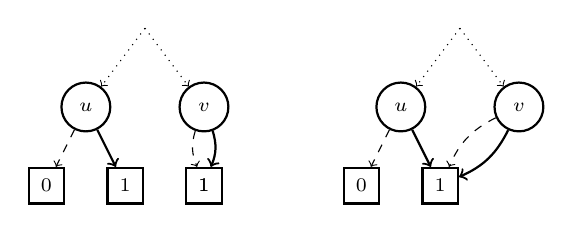
\begin{tikzpicture}[
        bdd/.style={circle, draw, thick, minimum size=0.62cm, inner sep=1pt},
        terminal/.style={rectangle, draw, thick, minimum width=0.45cm, minimum height=0.45cm},
        edge/.style={->, thick},
        every node/.style={font=\scriptsize}
      ]
      \node[bdd] (term_u) at (0.5,1) {\(u\)};
      \node[bdd] (term_v) at (2,1) {\(v\)};
      \node[terminal] (term_0) at (0,0) {0};
      \node[terminal] (term_1) at (1,0) {1};
      \node[terminal] (term_1b) at (2,0) {1};
      \node[terminal] (term_1c) at (2,0) {1};
      \draw[->, dotted] (1.25,2) -- (term_u);
      \draw[->, dotted] (1.25,2) -- (term_v);
      \draw[->, dashed] (term_u) -- (term_0);
      \draw[->, thick] (term_u) -- (term_1);
      \draw[->, dashed] (term_v) to[bend right=20] (term_1b);
      \draw[->, thick] (term_v) to[bend left=20] (term_1c);

      \node at (3,0.5) {\(\implies\)};
      \node[bdd] (term_u2) at (4.5,1) {\(u\)};
      \node[bdd] (term_v2) at (6,1) {\(v\)};
      \node[terminal] (term_02) at (4,0) {0};
      \node[terminal] (term_12) at (5,0) {1};
      \draw[->, dotted] (5.25,2) -- (term_u2);
      \draw[->, dotted] (5.25,2) -- (term_v2);
      \draw[->, dashed] (term_u2) -- (term_02);
      \draw[->, thick] (term_u2) -- (term_12);
      \draw[->, dashed] (term_v2) to[bend right=20] (term_12);
      \draw[->, thick] (term_v2) to[bend left=20] (term_12);
    \end{tikzpicture}
    \caption{Condivisione dei terminali}
  \end{figure}
  \item \keyword{eliminazione dei test ridondanti}: un nodo i cui due archi puntano allo stesso figlio può essere sostituito dal figlio stesso;
  \begin{figure}[H]
    \centering
    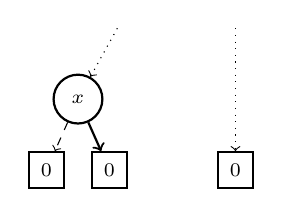
\begin{tikzpicture}[
        bdd/.style={circle, draw, thick, minimum size=0.62cm, inner sep=1pt},
        terminal/.style={rectangle, draw, thick, minimum width=0.45cm, minimum height=0.45cm},
        edge/.style={->, thick},
        every node/.style={font=\scriptsize}
      ]
      \node[bdd] (red_x) at (0,0) {\(x\)};
      \node[terminal] (red_0a) at (-0.4,-0.9) {0};
      \node[terminal] (red_0b) at (0.4,-0.9) {0};
      \draw[->, dotted] (0.5,0.9) -- (red_x);
      \draw[->, dashed] (red_x) -- (red_0a);
      \draw[->, thick] (red_x) -- (red_0b);
      \node at (1.4,0) {\(\implies\)};

        
      \node[terminal] (red_0c) at (2,-0.9) {0};
      \draw[->, dotted] (2,0.9) -- (red_0c);
    \end{tikzpicture}
    \caption{Eliminazione del test ridondante}
  \end{figure}
  \item \keyword{condivisione dei nodi interni}: se due nodi sono radici di sottodiagrammi isomorfi, se ne preserva uno solo, ridirigendo gli archi entranti nell'altro.
  \begin{figure}[H]
    \centering
    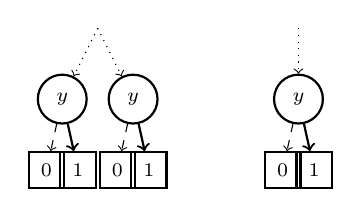
\begin{tikzpicture}[
        bdd/.style={circle, draw, thick, minimum size=0.62cm, inner sep=1pt},
        terminal/.style={rectangle, draw, thick, minimum width=0.45cm, minimum height=0.45cm},
        edge/.style={->, thick},
        every node/.style={font=\scriptsize}
      ]
      \node[bdd] (iso_y1) at (0,0) {\(y\)};
      \node[bdd] (iso_y2) at (0.9,0) {\(y\)};
      \node[terminal] (iso_0a) at (-0.2,-0.9) {0};
      \node[terminal] (iso_1a) at (0.2,-0.9) {1};
      \node[terminal] (iso_0b) at (0.7,-0.9) {0};
      \node[terminal] (iso_1b) at (1.1,-0.9) {1};
      \draw[->, dotted] (0.45,0.9) -- (iso_y1);
      \draw[->, dotted] (0.45,0.9) -- (iso_y2);
      \draw[->, dashed] (iso_y1) -- (iso_0a);
      \draw[->, thick] (iso_y1) -- (iso_1a);
      \draw[->, dashed] (iso_y2) -- (iso_0b);
      \draw[->, thick] (iso_y2) -- (iso_1b);

      \node at (1.8,0) {\(\implies\)};
      \node[bdd] (iso_y3) at (3,0) {\(y\)};
      \node[terminal] (iso_0c) at (2.8,-0.9) {0};
      \node[terminal] (iso_1c) at (3.2,-0.9) {1};
      \draw[->, dotted] (3,0.9) -- (iso_y3);
      \draw[->, dashed] (iso_y3) -- (iso_0c);
      \draw[->, thick] (iso_y3) -- (iso_1c);
    \end{tikzpicture}
    \caption{Condivisione dei nodi interni}
  \end{figure}
\end{itemize}

\begin{observation}{Località del test di isomorfismo}
  Il test di isomorfismo può sembrare costoso, perché sembrerebbe richiedere il confronto di interi sottodiagrammi. Ma se le regole si applicano dal basso verso l'alto, il test diventa \emph{locale}: due nodi sono radici di sottodiagrammi isomorfi se e solo se hanno la stessa etichetta e archi basso e alto che puntano rispettivamente agli stessi nodi. Infatti, se i sottodiagrammi dei figli erano isomorfi, sono già stati unificati da applicazioni precedenti della regola.
\end{observation}

\begin{example}{Trasformazione da Decision Tree a BDD}
  Vediamo dunque un esempio di trasformazione da albero di decisione a BDD, applicando le regole di riduzione. Consideriamo la banale funzione \(f(x,y,z) = x \lor (y\land z)\), il cui albero di decisione è:
  \begin{figure}[H]
    \centering
    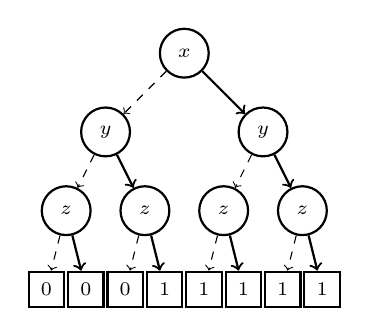
\begin{tikzpicture}[
        bdd/.style={circle, draw, thick, minimum size=0.62cm, inner sep=1pt},
        terminal/.style={rectangle, draw, thick, minimum width=0.45cm, minimum height=0.45cm},
        edge/.style={->, thick},
        every node/.style={font=\scriptsize}
      ]
      \node[bdd] (x) at (0,0) {\(x\)};
      \node[bdd] (y1) at (-1,-1) {\(y\)};
      \node[bdd] (y2) at (1,-1) {\(y\)};
      \node[bdd] (z1) at (-1.5,-2) {\(z\)};
      \node[bdd] (z2) at (-0.5,-2) {\(z\)};
      \node[bdd] (z3) at (0.5,-2) {\(z\)};
      \node[bdd] (z4) at (1.5,-2) {\(z\)};
      \node[terminal] (t0) at (-1.75,-3) {0};
      \node[terminal] (t1) at (-1.25,-3) {0};
      \node[terminal] (t2) at (-0.75,-3) {0};
      \node[terminal] (t3) at (-0.25,-3) {1};
      \node[terminal] (t4) at (0.25,-3) {1};
      \node[terminal] (t5) at (0.75,-3) {1};
      \node[terminal] (t6) at (1.25,-3) {1};
      \node[terminal] (t7) at (1.75,-3) {1};
      \draw[->, dashed] (x) -- (y1);
      \draw[->, thick] (x) -- (y2);
      \draw[->, dashed] (y1) -- (z1);
      \draw[->, thick] (y1) -- (z2);
      \draw[->, dashed] (y2) -- (z3);
      \draw[->, thick] (y2) -- (z4);
      \draw[->, dashed] (z1) -- (t0);
      \draw[->, thick] (z1) -- (t1);
      \draw[->, dashed] (z2) -- (t2);
      \draw[->, thick] (z2) -- (t3);
      \draw[->, dashed] (z3) -- (t4);
      \draw[->, thick] (z3) -- (t5);
      \draw[->, dashed] (z4) -- (t6);
      \draw[->, thick] (z4) -- (t7);
    \end{tikzpicture}
    \caption{Albero di decisione per \(f(x,y,z) = x \lor (y\land z)\)}
  \end{figure}
  Applichiamo ora le regole di riduzione, dal basso verso l'alto:
  \begin{figure}[H]
    \centering
    \begin{minipage}{0.3\textwidth}

      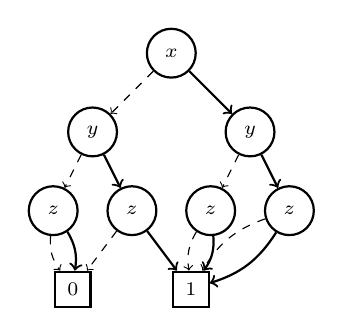
\begin{tikzpicture}[
        bdd/.style={circle, draw, thick, minimum size=0.62cm, inner sep=1pt},
        terminal/.style={rectangle, draw, thick, minimum width=0.45cm, minimum height=0.45cm},
        edge/.style={->, thick},
        every node/.style={font=\scriptsize}
        ]
      \node[bdd] (x) at (0,0) {\(x\)};
      \node[bdd] (y1) at (-1,-1) {\(y\)};
      \node[bdd] (y2) at (1,-1) {\(y\)};
      \node[bdd] (z1) at (-1.5,-2) {\(z\)};
      \node[bdd] (z2) at (-0.5,-2) {\(z\)};
      \node[bdd] (z3) at (0.5,-2) {\(z\)};
      \node[bdd] (z4) at (1.5,-2) {\(z\)};
      \node[terminal] (t0) at (-1.25,-3) {0};
      \node[terminal] (t1) at (0.25,-3) {1};
      \draw[->, dashed] (x) -- (y1);
      \draw[->, thick] (x) -- (y2);
      \draw[->, dashed] (y1) -- (z1);
      \draw[->, thick] (y1) -- (z2);
      \draw[->, dashed] (y2) -- (z3);
      \draw[->, thick] (y2) -- (z4);
      \draw[->, dashed] (z1) to[bend right=20] (t0);
      \draw[->, thick] (z1) to[bend left=20] (t0);
      \draw[->, dashed] (z2) -- (t0);
      \draw[->, thick] (z2) -- (t1);
      \draw[->, dashed] (z3) to[bend right=20] (t1);
      \draw[->, thick] (z3) to[bend left=20] (t1);
      \draw[->, dashed] (z4) to[bend right=20] (t1);
      \draw[->, thick] (z4) to[bend left=20] (t1);
    \end{tikzpicture}
  \end{minipage}
  \begin{minipage}{0.3\textwidth}
      
      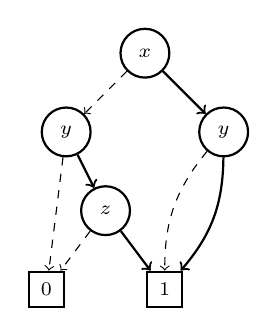
\begin{tikzpicture}[
        bdd/.style={circle, draw, thick, minimum size=0.62cm, inner sep=1pt},
        terminal/.style={rectangle, draw, thick, minimum width=0.45cm, minimum height=0.45cm},
        edge/.style={->, thick},
        every node/.style={font=\scriptsize}
        ]
      \node[bdd] (x) at (0,0) {\(x\)};
      \node[bdd] (y1) at (-1,-1) {\(y\)};
      \node[bdd] (y2) at (1,-1) {\(y\)};
      \node[bdd] (z2) at (-0.5,-2) {\(z\)};
      \node[terminal] (t0) at (-1.25,-3) {0};
      \node[terminal] (t1) at (0.25,-3) {1};
      \draw[->, dashed] (x) -- (y1);
      \draw[->, thick] (x) -- (y2);
      \draw[->, dashed] (y1) -- (t0);
      \draw[->, thick] (y1) -- (z2);
      \draw[->, dashed] (y2) to[bend right=20] (t1);
      \draw[->, thick] (y2) to[bend left=20] (t1);

      \draw[->, dashed] (z2) -- (t0);
      \draw[->, thick] (z2) -- (t1);

    \end{tikzpicture}
  \end{minipage}
  \begin{minipage}{0.3\textwidth}
      
      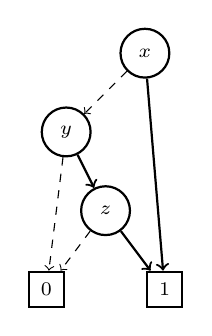
\begin{tikzpicture}[
        bdd/.style={circle, draw, thick, minimum size=0.62cm, inner sep=1pt},
        terminal/.style={rectangle, draw, thick, minimum width=0.45cm, minimum height=0.45cm},
        edge/.style={->, thick},
        every node/.style={font=\scriptsize}
        ]
     \node[bdd] (x) at (0,0) {\(x\)};
      \node[bdd] (y1) at (-1,-1) {\(y\)};
      \node[bdd] (z2) at (-0.5,-2) {\(z\)};
      \node[terminal] (t0) at (-1.25,-3) {0};
      \node[terminal] (t1) at (0.25,-3) {1};
      \draw[->, dashed] (x) -- (y1);
      \draw[->, thick] (x) -- (t1);
      \draw[->, dashed] (y1) -- (t0);
      \draw[->, thick] (y1) -- (z2);

      \draw[->, dashed] (z2) -- (t0);
      \draw[->, thick] (z2) -- (t1);

    \end{tikzpicture}
  \end{minipage}
  \caption{Riduzione dell'albero di decisione a BDD}
  \end{figure}
\end{example}

\section{OBDD: ordinamento e canonicità}

La rappresentazione BDD non è ancora canonica: per la stessa funzione è possibile scegliere una qualsiasi variabile per etichettare il nodo iniziale, ottenendo BDD completamente diversi; in linea di principio ogni ordinamento dei test porta a un grafo diverso. La forma canonica si ottiene fissando un ordinamento sulle variabili.

\begin{definition}{OBDD}
  Fissato un ordinamento totale \(x_1 \prec x_2 \prec \cdots \prec x_n\) sulle variabili, un \keyword{Ordered BDD} (OBDD) è un BDD in cui, su ogni percorso dal nodo iniziale ai terminali, le variabili compaiono rispettando l'ordinamento.
\end{definition}

\begin{theorem}{Canonicità}
  Fissato l'ordinamento sulle variabili, per ogni funzione booleana esiste un unico OBDD ridotto (ROBDD) che la rappresenta.
\end{theorem}

La canonicità è la proprietà chiave: il test di uguaglianza tra funzioni (e dunque tra insiemi, rappresentati dalle loro funzioni caratteristiche) si riduce a un test di isomorfismo tra OBDD, eseguibile in tempo lineare nelle dimensioni. In pratica si fa ancora meglio: l'eliminazione della ridondanza si applica all'intera \emph{foresta} di BDD di tutte le funzioni in uso, ammettendo più radici in un unico DAG condiviso. In questo modo due funzioni equivalenti fanno riferimento allo stesso oggetto, e la verifica di uguaglianza diventa costante: basta confrontare gli identificativi (puntatori).

\subsection{L'importanza dell'ordinamento}

L'ordine delle variabili non è importante solo per la canonicità, ma anche per la \emph{dimensione} del diagramma.

\begin{example}{}
  Consideriamo la funzione \(f = \bigwedge_{i=1}^n (x_i \leftrightarrow y_i)\). Con l'ordinamento \(x_1,y_1,x_2,y_2,\dots,x_n,y_n\) (variabili correlate adiacenti), l'OBDD ha dimensione \(3n + 2\), lineare. Con l'ordinamento \(x_1,x_2,\ldots, x_n,y_1,y_2, \ldots, y_n\), invece, la dimensione è \(3\cdot 2^n-1\), esponenziale.
  \begin{figure}[H]
      \centering
      \tikzset{
          bddnode/.style={circle, draw, minimum size=7mm, inner sep=0pt, font=\small},
          terminal/.style={rectangle, draw, minimum size=6mm, font=\small\bfseries},
          edge0/.style={->, dashed, thick},
          edge1/.style={->, solid, thick}
      }
      
      % PRIMO GRAFO: Ordinamento Lineare
      \begin{minipage}{0.45\textwidth}
          \centering
          \begin{tikzpicture}[>=stealth]
              % Nodi variabili
              \node[bddnode] (x1) at (0, 0) {\(x_1\)};
              
              \node[bddnode] (y1L) at (-1.2, -0.5) {\(y_1\)};
              \node[bddnode] (y1R) at (1.2, -0.5) {\(y_1\)};
              
              \node[bddnode] (x2) at (0, -1) {\(x_2\)};
              
              \node[bddnode] (y2L) at (-1.2, -1.5) {\(y_2\)};
              \node[bddnode] (y2R) at (1.2, -1.5) {\(y_2\)};
              
              % Terminali
              \node[terminal] (T1) at (0, -2) {1};
              \node[terminal] (T0) at (2.5, -2) {0};
              
              % Archi (edge0 = tratteggiato/falso, edge1 = solido/vero)
              \draw[edge0] (x1) -- (y1L);
              \draw[edge1] (x1) -- (y1R);
              
              \draw[edge0] (y1L) -- (x2);
              \draw[edge1] (y1L) to[bend left=15] (T0);
              
              \draw[edge0] (y1R) to[bend left=15] (T0);
              \draw[edge1] (y1R) -- (x2);
              
              \draw[edge0] (x2) -- (y2L);
              \draw[edge1] (x2) -- (y2R);
              
              \draw[edge0] (y2L) -- (T1);
              \draw[edge1] (y2L) to[bend right=50] (T0);
              
              \draw[edge0] (y2R) -- (T0);
              \draw[edge1] (y2R) -- (T1);
          \end{tikzpicture}
          \caption*{Ordine \(x_1, y_1, x_2, y_2\) (Dim: 8)}
      \end{minipage}\hfill
      % SECONDO GRAFO: Ordinamento Esponenziale
      \begin{minipage}{0.5\textwidth}
          \centering
          \begin{tikzpicture}[>=stealth]
              % Livello x1
              \node[bddnode] (x1) at (0, 0) {\(x_1\)};
              
              % Livello x2
              \node[bddnode] (x2L) at (-1.5, -1) {\(x_2\)};
              \node[bddnode] (x2R) at (1.5, -1) {\(x_2\)};
              
              % Livello y1 (4 nodi per memorizzare le combinazioni di x1, x2)
              \node[bddnode] (y1_00) at (-2.7, -2) {\(y_1\)};
              \node[bddnode] (y1_01) at (-0.9, -2) {\(y_1\)};
              \node[bddnode] (y1_10) at (0.9, -2) {\(y_1\)};
              \node[bddnode] (y1_11) at (2.7, -2) {\(y_1\)};
              
              % Livello y2
              \node[bddnode] (y2_0) at (-1.5, -3) {\(y_2\)};
              \node[bddnode] (y2_1) at (1.5, -3) {\(y_2\)};
              
              % Terminali
              \node[terminal] (T1) at (0, -4) {1};
              \node[terminal] (T0) at (0, -4.5) {0};
              
              % Archi x1 -> x2
              \draw[edge0] (x1) -- (x2L);
              \draw[edge1] (x1) -- (x2R);
              
              % Archi x2 -> y1
              \draw[edge0] (x2L) -- (y1_00);
              \draw[edge1] (x2L) -- (y1_01);
              \draw[edge0] (x2R) -- (y1_10);
              \draw[edge1] (x2R) -- (y1_11);
              
              % Archi y1 -> y2 / T0
              \draw[edge0] (y1_00) -- (y2_0);
              \draw[edge1] (y1_00) to[out=200, in=170] (T0);
              
              \draw[edge0] (y1_01) -- (y2_1);
              \draw[edge1] (y1_01) to[out=340, in=0] (T0);
              
              \draw[edge0] (y1_10) to[out=310, in=0] (T0);
              \draw[edge1] (y1_10) -- (y2_0);
              
              \draw[edge0] (y1_11) to[out=290, in=0] (T0);
              \draw[edge1] (y1_11) -- (y2_1);
              
              % Archi y2 -> Terminali
              \draw[edge0] (y2_0) -- (T1);
              \draw[edge1] (y2_0) to[bend right=10] (T0);
              
              \draw[edge0] (y2_1) to[bend left=10] (T0);
              \draw[edge1] (y2_1) -- (T1);
          \end{tikzpicture}
          \caption*{Ordine \(x_1, x_2, y_1, y_2\) (Dim: 11)}
      \end{minipage}
      \vspace{0.3cm}
      \caption*{Esempio visivo per \(n=2\).}
  \end{figure}
\end{example}

Sfortunatamente funzioni diverse hanno ordinamenti ottimali diversi, e decidere qual è l'ordinamento ottimale è un problema NP-completo. Nella pratica vengono adottate euristiche, senza però garanzia di ottenere OBDD compatti.

\begin{warning}{}
  Esistono funzioni (legate ad esempio alla moltiplicazione binaria) il cui OBDD è esponenziale per \emph{qualsiasi} ordinamento: la rappresentazione simbolica non è una bacchetta magica, e i collegamenti con SAT e VALIDITY (che su OBDD canonici si risolvono in tempo costante, guardando se l'OBDD è diverso da \(0\) o uguale a \(1\)) implicano che il costo esponenziale si scarica sulla \emph{costruzione} dell'OBDD.
\end{warning}

Applicando le regole di riduzione a un albero di decisione si ottiene un OBDD ridotto, o \keyword{ROBDD}.

\begin{definition}{ROBDD}
  Un \keyword{Reduced OBDD} (ROBDD) è un OBDD tale che:
  \begin{enumerate}
    \item esistono esattamente due vertici terminali, etichettati rispettivamente con \(1\) e \(0\);
    \item \[\forall v \in V, low(v)\neq high(v)\]
    \item \[\forall u,v \in V, low(u) = low(v) \land high(u) = high(v) \land var(u) = var(v) \implies u = v\]
  \end{enumerate}
\end{definition}

\subsection{Costruzione dei ROBDD}

Le regole di riduzione della obdd-canonicity descrivono \emph{quando} un BDD è ridondante, ma non dicono come costruire direttamente un OBDD già ridotto. L'approccio ingenuo — costruire prima l'intero albero di decisione e poi applicare le regole di riduzione dal basso verso l'alto, come sulla località del test di isomorfismo — funziona, ma è inutilmente costoso: l'albero di decisione completo ha sempre \(2^{n+1}-1\) nodi, indipendentemente da quanto l'OBDD finale sia piccolo. Vogliamo invece un procedimento che produca nodi \emph{già canonici}, senza mai passare per la rappresentazione intermedia esponenziale.

L'idea è mantenere \emph{due} tabelle, che rappresentano lo stesso insieme di nodi indicizzato in due modi complementari:
\begin{itemize}
  \item la \keyword{tabella del grafo} \(T\), indicizzata per identificatore di nodo, che associa a ogni nodo \(u\) la sua tripla \((var(u), low(u), high(u))\): è la rappresentazione del DAG vero e proprio, quella che si attraversa per valutare la funzione;
  \item la \keyword{tabella di hashing} \(H\) (o \emph{unique table}), indicizzata per tripla, che associa a \((x,l,h)\) l'identificatore del nodo con quella struttura, \emph{se già esiste}.
\end{itemize}
Le due tabelle sono l'una l'inversa dell'altra: \(T[u] = (x,l,h) \iff H[(x,l,h)] = u\). Servono entrambe le direzioni perché durante la costruzione bisogna sia navigare il DAG a partire da un nodo (\(T\)), sia chiedersi, prima di creare un nodo nuovo, se una struttura equivalente esiste già (\(H\)) — ed è proprio quest'ultimo controllo, se implementato con una tabella hash, a rendere il test in tempo atteso costante anziché lineare nel numero di nodi già creati.

\begin{algorithmdesc}{Creazione canonica di un nodo}
  \begin{algorithmic}[1]
    \Statex{} \textbf{signature} \(\textsc{Mk:} \quad Var \times NodeId \times NodeId \to NodeId\)
    \Function{\(\textsc{Mk}\)}{$x,l,h$} % chktex 46
    \If{\(l = h\)}
    \State{} \Return{} \(l\)
    \ElsIf{\((x,l,h) \in \mathrm{dom}(H)\)}
    \State{} \Return{} \(H[(x,l,h)]\)
    \Else{}
    \State{} \(u \gets FreshNodeId()\) \Comment{} ottieni un nuovo identificatore di nodo
    \State{} \(T[u] \gets (x,l,h)\)
    \State{} \(H[(x,l,h)] \gets u\)
    \State{} \Return{} \(u\)
    \EndIf{}
    \EndFunction{}
  \end{algorithmic}
\end{algorithmdesc}

La funzione \(\textsc{Mk}\) è l'\emph{unico} punto del procedimento in cui vengono creati nodi, e applica in un solo passaggio entrambe le regole di riduzione strutturale già viste: la condizione \(l=h\) è esattamente l'eliminazione dei test ridondanti (un nodo i cui due archi portano allo stesso figlio collassa nel figlio stesso, senza bisogno di distinguere il valore di \(x\)); il controllo su \(H\) è la condivisione dei nodi interni, e garantisce che due sottodiagrammi con struttura identica restino un unico nodo condiviso in memoria, mai duplicato. La condivisione dei terminali, invece, è garantita a monte: i nodi \(0\) e \(1\) vengono creati una sola volta in fase di inizializzazione e riutilizzati sempre come possibili valori di \(l,h\).

\begin{note}{}
  Chiamare \(\textsc{Mk}\) al posto di creare direttamente un nuovo nodo è ciò che rende l'intero procedimento canonico \emph{per costruzione}: non serve mai un passaggio separato di riduzione a posteriori, perché ogni nodo, nel momento stesso in cui viene richiesto, o riusa una struttura già presente o ne crea esattamente una, mai più di una, per ogni tripla distinta.
\end{note}

Con \(\textsc{Mk}\) a disposizione, la costruzione dell'OBDD di una funzione booleana \(f\) sulle variabili ordinate \(x_1 \prec \cdots \prec x_n\) procede seguendo esattamente l'espansione di Shannon: si calcolano ricorsivamente i due cofattori rispetto alla variabile corrente, si costruiscono i loro OBDD sulle variabili rimanenti, e li si richiude con \(\textsc{Mk}\).

\begin{algorithmdesc}{Build: costruzione dell'OBDD di una funzione}
  \begin{algorithmic}[1]
    \Statex{} \textbf{signature} \(\textsc{Build:} \quad BoolFun \times \mathbb{N} \to NodeId\)
    \Function{\(\textsc{Build}\)}{$f,i$} % chktex 46
    \If{\(i \succ n\)}
    \State{} \Return{} \(Terminal(1)\) se \(f \equiv 1\), \(Terminal(0)\) se \(f \equiv 0\)
    \Else{}
    \State{} \(v_0 \gets \textsc{Build}(f_{\overline{x_i}}, i+1)\)
    \State{} \(v_1 \gets \textsc{Build}(f_{x_i}, i+1)\)
    \State{} \Return{} \(\textsc{Mk}(x_i, v_0, v_1)\)
    \EndIf{}
    \EndFunction{}
  \end{algorithmic}
\end{algorithmdesc}

La correttezza si dimostra per induzione, procedendo dall'ultima variabile alla prima: se \(v_0\) e \(v_1\) sono già i ROBDD canonici dei rispettivi cofattori (base dell'induzione: i terminali sono banalmente canonici), allora \(\textsc{Mk}(x_i,v_0,v_1)\) restituisce il ROBDD canonico di \(f\), per lo stesso argomento di canonicità-per-costruzione appena discusso.

\begin{observation}{Complessità di Build}
  Così come presentato, \(\textsc{Build}\) nel caso peggiore effettua \(\BigO{2^n}\) chiamate ricorsive: una per ogni possibile assegnamento delle variabili, esattamente come nella costruzione dell'albero di decisione completo, perché i cofattori vengono ricalcolati indipendentemente lungo ogni ramo, senza alcuna cache sulle chiamate ricorsive stesse (solo \(\textsc{Mk}\) è cached, tramite \(H\)). Quello che si può fare è memorizzare i risultati parziali di \(\textsc{Build}\) in una tabella indicizzata da \((f,i)\), così che ogni coppia distinta venga calcolata una sola volta. In questo modo la complessità totale diventa \(\BigO{\abs{f}}\), dove \(\abs{f}\) è la dimensione dell'OBDD finale.
\end{observation}


\section{Operazioni sugli OBDD}

Per il model checking simbolico servono le operazioni insiemistiche (\(\cap, \cup\), complemento) sulle funzioni caratteristiche, e la preimmagine. Vediamo come implementarle.

\subsection{L'algoritmo Apply}

Dati gli OBDD di due funzioni \(f\) e \(g\), vogliamo calcolare l'OBDD di \(f \circ g\) per un operatore booleano binario \(\circ\). L'idea sfrutta il fatto che l'espansione di Shannon commuta con gli operatori booleani:
\begin{equation*}
  \begin{aligned}
    f \lor g & = ((x_1 \land f_{x_1}) \lor (\neg x_1 \land f_{\overline{x_1}})) \lor ((x_1 \land g_{x_1}) \lor (\neg x_1 \land g_{\overline{x_1}})) \\
             & = (x_1 \land (f_{x_1} \lor g_{x_1})) \lor (\neg x_1 \land (f_{\overline{x_1}} \lor g_{\overline{x_1}}))
  \end{aligned}
\end{equation*}
e lo stesso vale per \(\land\) e per la negazione (esprimibile come \(\neg f \equiv f \oplus 1 \equiv\)). Possiamo facilmente notare in oltre che, se \(f\) e \(g\) differiscono nella loro prima variabile discriminante, l'espansione di Shannon si applica solo a quella variabile, lasciando invariata l'altra funzione. In altre parole, la ricorsione scende solo sui sottoalberi che dipendono dalla variabile corrente. Infine, il caso base non è altro che rappresentato dall'applicazione dell'operatore booleano ai due valori terminali.

\begin{note}{Costruzione di ROBDD senza algoritmo Build}
  L'algoritmo \textsc{Apply} fornisce un metodo alternativo per costruire l'OBDD di una funzione booleana a partire da due funzioni più semplici, senza passare per la costruzione dell'albero di decisione completo. In particolare, se \(f\) e \(g\) sono già OBDD canonici, allora \(\textsc{Apply}(f,g,\circ)\) restituisce l'OBDD canonico di \(f \circ g\).
\end{note}

\todo[inline]{Aggiungere lo pseudocodice dell'algoritmo Apply dalle slide}

\begin{algorithmdesc}{Apply: operazioni binarie sugli OBDD}
  \begin{algorithmic}[1]
    \Statex{} \textbf{signature} \(\textsc{Apply:} \quad BoolOp \times NodeId \times NodeId \to NodeId\)
    \Function{\(\textsc{Apply}\)}{$\circ,u,v$} %chktex 46
      \Function{\(TerminalCase\)}{$\circ,u,v$} %chktex 46
        \If{\(isTerminal(u) \land isTerminal(v)\)}
          \State{} \Return{} \(True\)
        \EndIf{}
        \If{\(\circ = \land\)}
          \State{} \Return{} \(u = Terminal(0) \lor v = Terminal(0)\)
        \ElsIf{\(\circ = \lor\)}
          \State{} \Return{} \(u = Terminal(1) \lor v = Terminal(1)\)
        \ElsIf{\(\circ = \oplus\)}
          \State{} \Return{} \(u = Terminal(0) \lor v = Terminal(0) \lor v=u\)
        \EndIf{}
      \EndFunction{}
      \Function{\(\textsc{App}\)}{$u,v$} %chktex 46
        \If{\(TerminalCase(\circ,u,v)\)}
          \State{} \Return{} \(\circ(u,v)\) \Comment{} \(\circ\) è a corto circuito
        \EndIf{}
        \State{} \(low_u, high_u \gets u,u\)
        \State{} \(low_v, high_v \gets v,v\)
        \State{} \(var \gets var(u)\)
        \If{\(var(u) \leq var(v)\)}
          \State{} \(low_u, high_u \gets low(u), high(u)\)
        \EndIf{}
        \If{\(var(v) \leq var(u)\)}
          \State{} \(low_v, high_v \gets low(v), high(v)\)
          \State{} \(var \gets var(v)\)
        \EndIf{}
        \State{} \Return{} \(\textsc{Mk}(var, \textsc{App}(low_u, low_v), \textsc{App}(high_u, high_v))\)
      \EndFunction{}
      \State{} \Return{} \(\textsc{App}(u,v)\)
    \EndFunction{}
  \end{algorithmic}
  
\end{algorithmdesc}


\begin{note}{}
  Nei casi in cui uno dei due OBDD dipende da una variabile da cui l'altro non dipende, la ricorsione scende solo su quello che ne dipende, lasciando l'altro invariato.
\end{note}

L'algoritmo di base ha complessità \(\BigO{2^n}\), perché ripete più volte le stesse chiamate ricorsive. Il problema si risolve con programmazione dinamica: mantenendo una cache dei risultati parziali indicizzata dalle triple \((\circ,u,v)\), ogni chiamata ricorsiva viene eseguita una sola volta e le successive risolte con un lookup a tempo costante. Fissato \(\circ\), le chiamate distinte sono al più \(\abs{f}\cdot \abs{g}\), e dunque la complessità totale è \(\BigO{\abs{f}\cdot \abs{g}}\).

\subsection{Restrizione e quantificazione booleana}

Data \(f(x_1,\ldots,x_n)\), la \keyword{restrizione} rispetto a un assegnamento parziale calcola l'OBDD dei cofattori, ad esempio \(f_{x_i}\) e \(f_{\overline{x_i}}\). Anche questa operazione può essere riformulata in funzione di espansione di Shannon, ma non essendo un operazione binaria, non è direttamente implementabile con \textsc{Apply}.

La restrizione è particolarmente utile per le \keyword{Quantified Boolean Formulae} (QBF), formule booleane quantificate con semantica identica al prim'ordine su dominio booleano. Dal punto di vista funzionale:
\[\exists x_i.\, f(x_1, \ldots, x_n) \equiv f_{x_i} \lor f_{\overline{x_i}} \qquad \forall x_i.\, f(x_1, \ldots, x_n) \equiv f_{x_i} \land f_{\overline{x_i}}\]

Dunque utilizzando \textsc{Apply} con \(\lor\) e \(\land\) appropriatamente sulle restrizioni, è possibile implementare la quantificazione booleana.

Per il model checking simbolico di \(CTL\) sarà sufficiente \(\exists\) per la preimmagine, che è intrinsecamente una proprietà esistenziale. In contesti di logica alternante invece, come nei giochi visti nel \Cref{ch:atl}, la preimmagine può invece essere universale, richiedendo entrambe le restrizioni.

Per l'implementazione della restrizione diretta sugli OBDD possiamo analizzare la loro struttura ricorsiva. Sia \(y\) la variabile da fissare a \(1\) o \(0\), e sia \(f\) l'OBDD della funzione booleana con variabile iniiziale \(x\). Per calcolare \(f_y\) o \(f_{\overline{y}}\) è sufficiente analizzare la posizione di \(y\) rispetto alla variabile del nodo corrente \(x\), in particolare:
\begin{itemize}
  \item Se \(y = x\), allora la riduzione si risolve immediatamente: \(f_y = high(f)\) e \(f_{\overline{y}} = low(f)\);
  \item Se \(y \prec x\), allora \(y\) non compare in \(f\), e dunque \(f_y = f_{\overline{y}} = f\);
  \item Se \(y \succ x\), allora la riduzione si applica ricorsivamente ai due figli: \(f_y = x\to high(f)_y ,low(f)_y\) e \(f_{\overline{y}} = x\to high(f)_{\overline{y}} ,low(f)_{\overline{y}}\).
\end{itemize}

Algoritmicamente il terzo caso è implementabile tramite due chiamate ricorsive su \(high(f)\) e \(low(f)\) rispettivamente.

\begin{algorithmdesc}{Restrict: calcolo della restrizione di un OBDD}
  \begin{algorithmic}[1]
    \Statex{} \textbf{signature} \(\textsc{Restrict:} \quad NodeId \times Var \times Bool \to NodeId\)
    \Function{\(\textsc{Restrict}\)}{$f,y,b$} %chktex 46
      \If{\(isTerminal(f)\)}
        \State{} \Return{} \(f\)
      \EndIf{}
      \Function{\(Res\)}{$f$} %chktex 46
        \If{\(var(f) \succ i\)}
          \State{} \Return{} \(f\)
        \ElsIf{\(var(f) \prec i\)}
          \State{} \Return{} \(\textsc{Mk}(var(f), Res(low(f)), Res(high(f)))\)
        \Else{}\Comment{} \(var(f) = i\)
          \If{\(b = 0\)}
            \State{} \Return{} \(Res(low(f))\)
          \Else{}
            \State{} \Return{} \(Res(high(f))\)
          \EndIf{}
        \EndIf{}
      \EndFunction{}
      \State{} \Return{} \(Res(f)\)
    \EndFunction{}
  \end{algorithmic}
\end{algorithmdesc}

Anche in questo caso questa versione dell'algoritmo risulta essere esponenziale, ma utilizzando una cache per memorizzare i risultati parziali, la complessità diventa lineare nella dimensione dell'OBDD di partenza.

\section{Model checking simbolico di CTL}
Abbiamo tutti gli ingredienti per il model checking simbolico. L'input è una struttura di Kripke: dobbiamo capire come codificarne la topologia tramite OBDD\@.

\subsection{Codifica di stati e transizioni}
Sia \(K = (AP,S,S_0,R,\lambda)\) una struttura di Kripke, con \(S = \{s_1, \ldots, s_m\}\) e \(AP = \{p_1, \ldots, p_n\}\). Ogni stato \(s_i\) è etichettato da un sottoinsieme di proposizioni atomiche: \(\lambda(s_i) \subseteq AP\). Possiamo rappresentare ogni stato come un assegnamento booleano alle variabili \(x_1, \ldots, x_n\), dove \(x_j = 1\) se e solo se \(p_j \in \lambda(s_i)\). In altre parole, ogni stato è rappresentato dalla sua funzione caratteristica:
\[\forall s_i \in S: f_{s_i} = \bigwedge_{p_j \in \lambda(s_i)} x_j \land \bigwedge_{p_j \notin \lambda(s_i)} \neg x_j\]
tale rappresentazione è sufficiente anche per rappresentare il singleton di ogni stato, permettendo di rappresentare ogni insieme di stati \(S'\subseteq S\) come la disgiunzione delle funzioni caratteristiche dei singoli stati che lo compongono:
\[\forall S' \subseteq S: f_{S'} = \bigvee_{s_i \in S'} f_{s_i}\]

Tale costruzione assume che \(\lambda\) sia iniettiva, ovvero che stati diversi abbiano etichettature diverse.Se così non fosse, basterebbe aggiungere qualche proposizione atomica fresca per distinguerli.

Di conseguenza, si ha che \(S \subseteq 2^{AP}\), e dunque \(\abs{S} \leq 2^n\). In oltre, essendo \(R \subseteq S \times S\), si ha che \(\abs{R} \leq 2^{2n}\). Di conseguenza tale rappresentazione, pur rimanendo lineare nella dimensione del grafo sottostante alla struttura di Kripke, rischia di essere esponenziale nel numero di proposizioni atomiche. In pratica, però, casi reali hanno una struttura molto regolare, e la rappresentazione simbolica tramite OBDD è spesso molto più compatta della rappresentazione esplicita.

Per la relazione di transizione \(R\subseteq S\times S\), avendo già la rappresentazione degli stati con le variabili \(x_1, \ldots, x_{n}\), è sufficiente raddoppiare le variabili introducendo \(x_1', \ldots, x_{n}'\) (\keyword{variabili primate}) e costruire un OBDD \(f_R\) che dipende da entrambe le sequenze: le variabili non primate rappresentano lo stato di partenza, quelle primate lo stato di arrivo. Se ad esempio \((s_1,s_2)\in R\), con \(L(s_1)=\{p,q\}\) e \(L(s_2)=\{r\}\), il termine corrispondente è
\[f_R(s_1,s_2) = f_{s_1}\land f'_{s_2} = (p\land q\land\neg r)\land(p'\land q'\land\neg r')\]
e \(f_R\) è l'OR di questi termini su tutte le coppie in \(R\):
\[f_R = \bigvee_{(s_1,s_2)\in R} f_R(s_1,s_2)\]

\begin{example}{}
  Consideriamo una struttura di Kripke con \(AP= \{p,q,r,t\}\), \(S = \{s_1, s_2, s_3\}\) e \(R = \{(s_1,s_2), (s_1,s_3), (s_2,s_1), (s_3,s_3)\}\). Fissando una codifica posizionale, la rappresentazione booleana dei singoli stati è:
  \begin{align*}
    f_{s_1} & = p \land q \land \neg r \land \neg t \\
    f_{s_2} & = p \land \neg q \land r \land \neg t \\
    f_{s_3} & = \neg p \land \neg q \land r \land t
  \end{align*}
  La relazione di transizione globale \(f_R\) si ottiene come disgiunzione delle transizioni puntuali, affiancando le variabili di stato corrente a quelle di stato successivo (\(v'\)):
  \begin{align*}
    f_R & = (f_{s_1} \land f'_{s_2}) \lor (f_{s_1} \land f'_{s_3}) \lor (f_{s_2} \land f'_{s_1}) \lor (f_{s_3} \land f'_{s_3}) \\
        & = (p \land q \land \neg r \land \neg t \land p' \land \neg q' \land r' \land \neg t') \lor\\
        & \quad (p \land q \land \neg r \land \neg t \land \neg p' \land \neg q' \land r' \land t') \lor \\
        & \quad (p \land \neg q \land r \land \neg t \land p' \land q' \land \neg r' \land \neg t') \lor \\
        & \quad (\neg p \land \neg q \land r \land t \land \neg p' \land \neg q' \land r' \land t')
  \end{align*}

  Sebbene in questo esempio didattico la formula espliciti tutti i 32 letterali corrispondenti ai 4 archi del grafo, la rappresentazione in memoria tramite OBDD opererà una drastica riduzione spaziale. Utilizzando un ordinamento di \emph{interleaving} delle variabili (\(p \prec p' \prec q \prec q' \dots\)), il processo di riduzione dell'OBDD identificherà e fonderà i sotto-grafi isomorfi. Ad esempio, i fattori comuni ricorrenti come la transizione \((\neg t \land \neg t')\) condivisa dai primi tre archi, verranno rappresentati da un unico percorso nel grafo decisionale, dimostrando la capacità della struttura simbolica di astrarre e comprimere le regolarità del modello rispetto a un'enumerazione esplicita in memoria.

\end{example}

\begin{note}{}
  Per l'ordinamento conviene alternare ogni variabile con la sua primata (\(x_1 \prec x_1' \prec x_2 \prec x_2' \prec \cdots\)), essendo strettamente correlate: come visto nell'esempio sull'ordinamento, tenere lontane variabili correlate fa esplodere la dimensione dell'OBDD\@.
\end{note}

\subsection{L'algoritmo simbolico}
Costruiamo induttivamente l'OBDD della denotazione \(\den{\phi}\) di ogni sottoformula:
\begin{itemize}
  \item per le proposizioni atomiche, \(\den{p_i}=f_{p_i}(x_1,\ldots,x_n)=x_i\) è l'OBDD della variabile corrispondente;
  \item per gli operatori booleani, si applica \textsc{Apply} con l'operatore corrispondente agli OBDD delle sottoformule: \(\den{\neg\phi}=f_{\phi}\oplus 1\), \(\den{\phi\land\psi}=f_{\phi}\land f_{\psi}\), e analogamente per \(\lor\);
  \item per \(EX\phi\), serve la preimmagine simbolica (detta anche \keyword{relational product}): si prende \(f_{\phi}(x_1,\ldots,x_n)\), la si \emph{rinomina} sulle variabili primate ottenendo \(f_{\phi}(x_1', \ldots, x_n')\) (in modo da interpretarla sugli stati di arrivo), la si interseca con \(f_{R}\), e si proietta via lo stato di arrivo con la quantificazione esistenziale\footnote{L'operazione può essere resa molto più efficiente applicando la quantificazione esistenziale \emph{eagerly}, ovvero spingendola più in basso possibile nella struttura, al primo punto in cui la variabile quantificata compare, in modo da ridurre la dimensione degli OBDD intermedi.}:
  \[\den{EX\phi}= \exists x_1',\ldots,x_n'.\ \left(f_{\phi}(x_1',\ldots,x_n')\land f_{R}(x_1,\ldots,x_n,x_1',\ldots,x_n')\right)\]
  \item per \(E(\phi_1 U \phi_2)\) ed \(EG\phi\), si applicano gli algoritmi di punto fisso di~\Cref{ch:ctl}, in cui ogni iterazione è ora interamente simbolica:
        \[\den{E(\phi_1U\phi_2)} = \mu Z.\big(f_{\phi_2} \lor (f_{\phi_1}\land\den{EX\,Z})\big) \qquad \den{EG\phi} = \nu Z.\big(f_{\phi}\land\den{EX\,Z}\big)\]
        dove \(\den{EX\,Z}\) è la preimmagine simbolica appena vista applicata a \(Z\), unioni e intersezioni sono \textsc{Apply}, e il test di stabilizzazione \(f_j = f_{j-1}\) è il confronto di puntatori garantito dalla canonicità.
\end{itemize}

\begin{algorithmdesc}{Compute\_EG}
  \begin{algorithmic}[1]
    \Statex{} \textbf{signature} \(\textsc{Compute\_EG:} \quad Formula \to OBDD\)
    \Function{\(\textsc{Compute\_EG}\)}{$\beta$} % chktex 46
    \State{} \(f_1(x) \gets f_\beta(x)\)
    \State{} \(j \gets 1\)
    \Repeat{}
    \State{} \(j \gets j+1\)
    \State{} \(f_j(x) \gets f_\beta(x) \land \exists x'.\big(f_R(x,x') \land f_{j-1}(x')\big)\)
    \Until{\(f_j(x) = f_{j-1}(x)\)}
    \State{} \Return{} \(f_j\)
    \EndFunction{}
  \end{algorithmic}
\end{algorithmdesc}

\begin{algorithmdesc}{Compute\_EU}
  \begin{algorithmic}[1]
    \Statex{} \textbf{signature} \(\textsc{Compute\_EU:} \quad Formula \times Formula \to OBDD\)
    \Function{\(\textsc{Compute\_EU}\)}{$\beta_1,\beta_2$} % chktex 46
    \State{} \(f_1(x) \gets f_{\beta_2}(x)\)
    \State{} \(j \gets 1\)
    \Repeat{}
    \State{} \(j \gets j+1\)
    \State{} \(f_j(x) \gets f_{\beta_2}(x) \lor \Big(f_{\beta_1}(x) \land \exists x'.\big(f_R(x,x') \land f_{j-1}(x')\big)\Big)\)
    \Until{\(f_j(x) = f_{j-1}(x)\)}
    \State{} \Return{} \(f_j\)
    \EndFunction{}
  \end{algorithmic}
\end{algorithmdesc}

Di conseguenza, data una formula \(CTL\) \(\phi\) e una struttura di Kripke \(K\), verificare se \(K \models \phi\) si riduce a calcolare l'OBDD di \(\den{\neg\phi}\) e verificare se \(f_{\neg\phi} \land f_{S_0} \neq 0\), ovvero se esiste uno stato iniziale che soddisfa la formula. In pratica, si calcola \(f_{\neg\phi}\) e lo si interseca con \(f_{S_0}\) mediante \(\textsc{Apply}(\land)\) per poi verificare a tempo costante se l'OBDD risultante è diverso da \(0\).

\begin{note}{}
  In entrambi gli algoritmi, il passo di iterazione \(\exists x'.(f_R(x,x')\land f_{j-1}(x'))\) è esattamente \(\den{EX\,f_{j-1}}\): gli algoritmi sono la stessa iterazione di Kleene vista in~\Cref{ch:ctl} per \(\mu V.f_U(V)\) e \(\nu V.f_G(V)\), qui resa esplicita come pseudocodice, con il test di terminazione \(f_j=f_{j-1}\) risolto a tempo costante grazie alla canonicità dei ROBDD.
\end{note}

\chapter{Modellazione di Sistemi a Tempo Continuo}

La modellazione vista finora si è concentrata su sistemi discreti, in cui il tempo avanza concettualmente a \q{scatti} in corrispondenza dell'esecuzione delle transizioni atomiche. Esiste tuttavia un'ampia classe di sistemi la cui correttezza dipende crucialmente dallo scorrere del \keyword{tempo reale} e dall'evoluzione di grandezze fisiche continue.

L'idea fondamentale per modellare tali sistemi è iniettare all'interno del formalismo discreto delle variabili che non evolvono in base ad assegnamenti discreti operati dal software, ma in base a leggi matematiche che dipendono dal tempo (es.\ temperatura, velocità, pressione).

\begin{definition}{Variabile Tempo Reale}
  Introduciamo una singola variabile continua per rappresentare il tempo assoluto, che denoteremo tipicamente con \(t\). A differenza delle variabili di programma classiche, il cui dominio è spesso finito o numerabile, la variabile tempo varia nel dominio dei numeri reali non negativi:
  \[ \text{dom}(t) = \R_{\ge 0} \]
  Questa variabile evolve autonomamente con derivata unitaria (\(\dot{t} = 1\)), misurando il tempo reale trascorso.
\end{definition}

\begin{observation}{Esplosione dello Spazio degli Stati e Decidibilità}
  L'introduzione di una variabile a dominio continuo altera drasticamente la trattabilità matematica e computazionale del modello.

  Ricordiamo che in un Transition System generato da variabili, lo spazio degli stati \(S\) è dato (o contiene) l'insieme di tutte le possibili valutazioni delle variabili. Una funzione di valutazione \(\eta\) mappa l'insieme delle variabili \(\Var\) nel loro dominio \(D\):
  \[ \eta: \Var \to D \]
  Se l'unica variabile di interesse è il tempo (\(\Var = \{t\}\)) e il dominio è \(D = \R_{\ge 0}\), il numero totale di valutazioni distinte corrisponde al numero di funzioni possibili:
  \[ \abs{D}^{\abs{\Var}} = \abs{\R_{\ge 0}}^1 = \abs{\R_{\ge 0}} \]
  Questo significa che lo spazio degli stati del sistema non è più finito, né numerabilmente infinito (come \(\N\)), ma possiede la cardinalità del continuo (non numerabile).

  Dal punto di vista pratico dell'Automated Software Verification, questo genera una barriera computazionale enorme. Gli algoritmi classici di verifica (Model Checking), che si basano sull'esplorazione esaustiva degli stati raggiungibili, falliscono in presenza di uno spazio non numerabile. Il problema della verifica per modelli con variabili continue diviene, in linea di principio, \keyword{indecidibile}. Sarà pertanto necessario introdurre tecniche formali di \keyword{astrazione} avanzate per ricondurre questo spazio continuo a un sistema finito equivalente ai fini della verifica, tema che verrà esplorato nello studio dei \keyword{Timed Automata}.
\end{observation}

Per modellare adeguatamente i sistemi \keyword{embedded} ovvero sistemi di controllo immersi in un ambiente analogico in cui le reazioni dipendono strettamente dalle tempistiche del mondo fisico il formalismo puramente discreto degli LTS risulta insufficiente. Si introduce pertanto un nuovo modello matematico: gli \keyword{Automi Temporizzati}. Questo modello arricchisce la struttura dei classici automi a stati finiti con variabili a dominio continuo che scorrono autonomamente misurando il progresso del tempo reale.

Supponiamo di voler progettare un controllore per un passaggio a livello. Questo sistema ha una parte digitale, il controllore, e una parte analogica, gli attuatori e i sensori (il treno, le sbarre).

\begin{figure}[H]
  \centering
  \includegraphics[width=0.8\textwidth]{_images/railroad_crossing_example.png}
  \caption{Componenti digitali e analogiche di un passaggio a livello.}
\end{figure}

Se usassimo il modello classico, la composizione sarebbe semplicemente asincrona con interleaving, ma questo porterebbe a comportamenti ammessi dal modello ma non desiderabili: ad esempio, il treno che attraversa il passaggio a livello prima che le sbarre si siano abbassate.

\begin{figure}[H]
  \centering
  \includegraphics[width=0.8\textwidth]{_images/railroad_bad_computation_tree.png}
  \caption{Computation tree con il comportamento indesiderato.}
\end{figure}

Quello che vorremmo è che il treno mandi il segnale di avvicinamento sufficientemente prima di arrivare al passaggio a livello: è quindi necessario poter specificare che le azioni impieghino un certo tempo per essere eseguite, che certe azioni possano essere abilitate solo dopo un certo tempo, o che debbano avvenire entro un certo tempo. Se queste tempistiche vengono garantite, il comportamento indesiderato non è più ammesso, e il modello è più fedele.

\begin{figure}[H]
  \centering
  \includegraphics[width=0.8\textwidth]{_images/railroad_crossing_rudimental_timing.png}
  \caption{Modellazione rudimentale di tempistiche per il passaggio a livello.}
\end{figure}

\begin{note}{}
  Anche quando due vincoli temporali riguardano una stessa transizione sincronizzante, a livello di modellazione è importante che restino due vincoli distinti su sottomodelli diversi, piuttosto che accorparli in un unico vincolo. Nella fase di modellazione ogni sottomodello deve occuparsi di descrivere il sottocomponente specifico e le sue caratteristiche: il comportamento complessivo del sistema dev'essere corretto grazie a proprietà \emph{emergenti} dalla composizione dei sottomodelli.
\end{note}

\section{Sintassi degli Automi Temporizzati}

Il problema della modellazione e della verifica di sistemi embedded è che il tempo è intrinsecamente denso, e quindi non è possibile modellarlo come un insieme discreto di stati.

Come per passare da automi a stati finiti ad automi a pila, partiremo quindi da un automa a stati finiti e aggiungiamo una struttura dati: in questo caso dei \keyword{clock} (cronometri), variabili a valori reali non negativi che possono essere scritte solo in un modo molto limitato, ovvero resettate a zero, ma mai assegnate a valori arbitrari.

Matematicamente possiamo vedere un clock come una funzione \(x: \R^+ \to \R^+\) del tempo reale, tale che \(\frac{d x(t)}{dt} = 1\).\footnote{Ciò che conta è che la derivata sia una costante positiva uguale per tutti i clock, ovvero che tutti i clock crescano alla stessa velocità: tale costante può essere presa come unità di misura del tempo, e dunque assunta pari a \(1\) senza perdita di generalità.} Le transizioni possono avere guardie costituite da vincoli sui clock, e come unica azione sui clock possono resettarne alcuni a zero. Per semplicità di trattazione consideriamo solo guardie sui clock, sebbene in linea di principio le guardie su variabili viste in precedenza restino ammesse.

\begin{definition}{Vincoli sui clock}
  Dato un insieme di clock \(C\), i vincoli \(\Phi(C)\) sono generati dalla grammatica:
  \[\phi ::= \top \mid x<c\mid x\leq c\mid x > c \mid x \geq c \mid \phi \land \phi\]
  con \(x \in C\) e \(c\) costante in un dominio numerabile, ad esempio \(c \in \N\) o \(c \in \Q\).
\end{definition}

\begin{observation}{}
  Non è ammessa la negazione (per questo sono inclusi tutti i confronti di disuguaglianza) e non è presente la disgiunzione, che viene modellata tramite più transizioni parallele aventi come guardie i diversi disgiunti. Le costanti non possono essere in \(\R\), poiché ciò porterebbe a problemi di rappresentazione e computazione.
\end{observation}

\begin{note}{}
  Il modello è aperto a diverse estensioni:
  \begin{itemize}
    \item vincoli \q{triangolari} come \(x-y \leq c\): non cambiano l'espressività;
    \item vincoli con somme o prodotti come \(x+y \leq c\): aumentano l'espressività e la complessità dei problemi di decisione;
    \item reset a un valore costante diverso da zero, \(x := c\): non aumenta espressività né complessità;
    \item reset al valore di un altro clock, \(x := y\): aumenta espressività e complessità.
  \end{itemize}
  In generale, i vincoli scelti sono rilassabili per guadagnare succintezza, ma non espressività, senza esplosione della complessità.
\end{note}

\begin{definition}{Automa Temporizzato}
  Un \keyword{automa temporizzato} è una tupla
  \[TA = \langle\Sigma, \Loc, \Loc_0, C, \delta, F\rangle\]
  dove:
  \begin{itemize}
    \item \(\Sigma\) è l'alfabeto;
    \item \(\Loc\) è l'insieme delle locazioni;
    \item \(\Loc_0 \subseteq \Loc\) è l'insieme delle locazioni iniziali;
    \item \(C\) è l'insieme dei clock;
    \item \(F\subseteq \Loc\) è l'insieme delle locazioni finali;
    \item \(\delta \subseteq \Loc \times \Sigma \times \Phi(C) \times 2^C \times \Loc\) è la relazione di transizione
  \end{itemize}
  In particolare, si ha che se \((\ell, a, \phi, C',\ell') \in \delta\) allora esiste una transizione da \(\ell\) a \(\ell'\) etichettata con \(a\), abilitata solo se la guardia \(\phi\) è soddisfatta, e che resettando i clock in \(C'\).
\end{definition}

\begin{example}{Automa Temporizzato per un interruttore}
  \begin{figure}[H]
    \centering
    \includegraphics[width=0.5\textwidth]{_images/lightswitch_1}
    \caption{Automa a stati finiti per un interruttore.}
  \end{figure}
  \begin{figure}[H]
    \centering
    \includegraphics[width=0.5\textwidth]{_images/lightswitch_2}
    \caption{Automa temporizzato per un interruttore.}
  \end{figure}
\end{example}

\section{Semantica degli Automi Temporizzati}

Come per i program graphs, per dare una semantica agli automi temporizzati faremo affidamento ai transition system, in particolare in questo caso ai \keyword{timed transition system}, che ci permetteranno facilmente di definire le strutture di Kripke e quindi di applicare le tecniche di model checking viste negli scorsi capitoli.

Gli stati di un timed transition system sono coppie \((\ell, \nu)\) dove \(\ell\) è una locazione e \(\nu\) è una funzione di valutazione dei clock \(\nu: C \to \R_{\ge 0}\).

La relazione di transizione tra stati può essere dovuta sia alla lettura di un simbolo che al passare del tempo: le azioni sono dunque \(\Act = \Sigma \cup \R^+\), e le transizioni sono di due tipi:
\begin{itemize}
  \item \keyword{transizioni discrete}, etichettate con simboli di \(\Sigma\), da \((\ell,\nu)\) a \((\ell',\nu')\): cambiano locazione e possono azzerare alcuni clock;
  \item \keyword{transizioni di scorrimento del tempo}, etichettate con \(d \in \R^+\), da \((\ell,\nu)\) a \((\ell,\nu + d)\): la locazione resta invariata e tutti i clock avanzano di \(d\).
\end{itemize}

In particolare avremo che \((\ell,\nu) \xrightarrow{a} (\ell',\nu')\) se e sono se \((\ell, a,\phi, C',\ell') \in \delta\) per qualche \(\phi \in \Phi(C)\) e \(C'\subseteq C\) tali che \(\nu \models \phi\) e \(\nu' = \nu[C' \gets 0]\), ovvero \(\nu'\) è la funzione di valutazione dei clock ottenuta da \(\nu\) resettando a zero i clock in \(C'\) e la relazione \(\nu \models \phi\) è definita nel modo ovvio.

Per quanto riguarda le transizioni di scorrimento del tempo, avremo che \((\ell,\nu) \xrightarrow{d} (\ell,\nu + d)\) dove \(\nu + d: C \to \R_{\ge 0}\) è la funzione di valutazione dei clock definita da \((\nu + d)(x) = \nu(x) + d\) per ogni \(x \in C\).

\section{Linguaggi temporizzati e \texorpdfstring{\(\tau\)}{tau}-transizioni}

In termini di teoria dei linguaggi, questi automi riconoscono \keyword{linguaggi temporizzati}, in cui gli elementi delle parole sono detti \keyword{segnali}: coppie di un simbolo di alfabeto e dell'istante di tempo in cui viene emesso.

Una \keyword{traccia temporizzata} è una sequenza (potenzialmente infinita) di segnali \(\sigma = (a_1,t_1)(a_2,t_2)\ldots\) con \(a_i \in \Sigma\) e \(t_i \in \R^+\) tali che \(t_i \leq t_{i+1}\) per ogni \(i\in\N\). 

Un run di un automa temporizzato con stato iniziale \((\ell_0,\nu_0)\) su una traccia temporizzata \(\sigma=(a_1,t_1)(a_2,t_2)\ldots\) è una sequenza di transizioni del timed transition system:
\[(\ell_0,\nu_0) \xrightarrow{d_1}\xrightarrow{a_1} (\ell_1,\nu_1) \xrightarrow{t_2}\xrightarrow{a_1} (\ell_2,\nu_2) \ldots\]
tale che \(t_{i+1} - t_i = d_{i+1}\) per ogni \(i\in\N\).

\begin{note}{}
  Nei percorsi temporizzati, per ogni transizione temporale di ritardo \(d\) esistono infiniti modi equivalenti di sezionarla in sotto-transizioni: per ogni coppia \(d_1, d_2\) con \(d=d_1+d_2\), la transizione di ritardo \(d\) equivale alla sequenza delle due transizioni di ritardo \(d_1\) e \(d_2\).

  \begin{figure}[H]
    \centering
    \includegraphics[width=0.5\textwidth]{_images/temporal_traces.png}
    \caption{Tracce temporizzate equivalenti, con transizioni di ritardo sezionate in modi diversi. La sezione tra barre rosse evidenzia le transizioni discrete}
  \end{figure}
\end{note}

In questo modello le transizioni discrete avvengono solo in risposta a stimoli esterni (lettura di un simbolo). Per modellare transizioni \emph{spontanee} aggiungiamo le \keyword{\(\tau\)-transizioni}: un simbolo speciale \(\tau\) che indica una transizione senza stimolo esterno.

\begin{warning}{}
  A differenza delle \(\epsilon\)-transizioni negli automi a stati finiti, le \(\tau\)-transizioni \emph{aumentano} il potere espressivo degli automi temporizzati.
\end{warning}

\begin{example}{}
  Consideriamo un automa con una \(\tau\)-transizione con guardia \(x = 1\) e reset di \(x\), che quindi può azzerare spontaneamente il clock a ogni istante intero. Tale automa può riconoscere il linguaggio delle parole \((a,t_1)(a,t_2)\ldots\) con tutti i \(t_i \in \N\): a ogni istante intero il clock può essere azzerato, permettendo di \q{scandire} tutti gli interi. Nessun automa temporizzato senza \(\tau\)-transizioni può riconoscere lo stesso linguaggio: senza la possibilità di azzerare spontaneamente il clock, si può solo verificare che tra due simboli letti ci sia una specifica distanza, non scandire tutti gli interi.
  
  \begin{figure}[H]
    \centering
    \includegraphics[width=0.5\textwidth]{_images/tau-timed_automata_counting_naturals.png}
    \caption{Automa temporizzato con \(\tau\)-transizione che riconosce il linguaggio delle parole con simboli letti a istanti interi.}
  \end{figure}
\end{example}

\section{Invarianti, timelock e zenoness}

Il modello manca ancora di qualcosa: possiamo impedire che una transizione avvenga prima o dopo un certo tempo (abilitarla in un intervallo), ma non possiamo \emph{forzare} che una transizione avvenga entro un certo tempo. Le \(\tau\)-transizioni danno la possibilità che qualcosa accada spontaneamente, ma non l'obbligo.

Consideriamo ad esempio l'automa in figura:

\begin{figure}[H]
  \centering
  \includegraphics[width=0.5\textwidth]{_images/exceding_time_example.png}
  \caption{Automa temporizzato con transizione che deve avvenire entro un certo tempo.}
\end{figure}

Dal grafico ad esso affiancato, che rappresenta una possibile evoluzione del clock \(x\) nel tempo, è facile vedere che non è possibile in alcun modo garantire che la transizione avvenga in tempo: se il sistema resta nello stato iniziale per più di \(3\) unità di tempo, la guardia della transizione non sarà più soddisfatta e il sistema si bloccherà.

\begin{definition}{Invarianti}
  Una funzione di \keyword{invariante} \(Inv: \Loc \to \Phi(C)\) associa un vincolo sui clock a ogni locazione, con la semantica di limitare il tempo che è possibile trascorrervi: se \(Inv(l) = x \leq c\), è possibile rimanere in \(l\) solo finché \(x \leq c\).
\end{definition}

Il senso è considerare \emph{spurio} (e dunque escludere) ogni percorso che violerebbe un'invariante. La semantica va aggiornata di conseguenza:
\begin{itemize}
  \item le transizioni di scorrimento del tempo sono ammesse solo se il passaggio soddisfa l'invariante: \(\nu + d \models Inv(l)\);\footnote{Più precisamente, l'invariante deve valere lungo tutto lo scorrimento; per vincoli convessi come i nostri è sufficiente verificarla all'istante finale.}
  \item le transizioni discrete devono garantire che la valutazione risultante soddisfi l'invariante della locazione di arrivo: \(\nu' \models Inv(l')\).
\end{itemize}

L'aggiunta delle invarianti permette di modellare le \emph{durate} delle azioni, oltre ai ritardi già esprimibili con le guardie.

Per quanto riguarda la composizione di automi temporizzati, avendo considerato il caso senza variabili, si utilizza il modello di sincronizzazione con handshaking: le transizioni sincronizzanti sono quelle con lo stesso simbolo di alfabeto, le altre sono asincrone.

\subsection{Problemi di modellazione}

L'introduzione del tempo continuo porta con sé alcuni fenomeni patologici da conoscere:
\begin{itemize}
  \item la \keyword{time convergence}, inevitabile, ma gestibile in fase di verifica;
  \item il \keyword{timelock}, introdotto dalle invarianti;
  \item la \keyword{zenoness}, in cui infinite azioni avvengono in un intervallo di tempo finito.
\end{itemize}

\begin{definition}{Percorsi convergenti e divergenti}
  Dato un percorso infinito \(\pi\) con ritardi \(d_1, d_2, \ldots\), il suo tempo di esecuzione è \(ExecTime(\pi) = \sum_{i \geq 1} d_i\). Il percorso è \keyword{convergente} se \(ExecTime(\pi)<\infty\), \keyword{divergente} altrimenti. Dato uno stato \(s\), indichiamo i percorsi divergenti da \(s\) con
  \[Paths_{div}(s) = \set{\pi}[\pi_0 = s \land ExecTime(\pi) =\infty]\]
\end{definition}

\begin{example}{}
  Un percorso che a ogni passo lascia scorrere ritardi \(d_i = \frac{1}{2^i}\) ha \(ExecTime(\pi) = \sum_{i \geq 1} \frac{1}{2^i} = 1\): il tempo del percorso converge a un valore finito nonostante il percorso sia infinito.
\end{example}

I percorsi convergenti con un numero \emph{finito} di transizioni discrete possono essere ignorati senza perdita: le infinite transizioni temporali si accorpano in un'unica transizione con ritardo pari al limite della somma. Nella verifica ci interesseremo dunque solo dei percorsi divergenti.

\begin{definition}{Timelock}
  Uno stato \(s\) è un \keyword{timelock} se \(Paths_{div}(s) = \emptyset\), ovvero se non esiste alcun percorso divergente che parte da \(s\).
\end{definition}

Un timelock non significa che da \(s\) non parta alcun percorso o che il sistema non evolva, ma che tutti i percorsi da \(s\) sono convergenti: il tempo non può più procedere oltre un certo limite. È la controparte temporale del deadlock: il sistema deve evolvere perché sta per raggiungere una deadline dovuta a un'invariante, ma tutte le transizioni sono disabilitate.

\begin{definition}{Zenoness}
  Un percorso \(\pi\) è \keyword{zeno} se \(ExecTime(\pi)<\infty\) e il numero di transizioni discrete in \(\pi\) è infinito. Un automa temporizzato è \keyword{non-zeno} se non ammette percorsi zeno.
\end{definition}

I percorsi zeno rappresentano un sistema con velocità di esecuzione arbitrariamente alta, fisicamente irrealizzabile: sono possibili perché le transizioni discrete sono istantanee, e quelle spontanee non necessitano nemmeno di uno stimolo esterno. Verificare l'assenza di zenoness è un problema difficile, ma esiste una comoda condizione sufficiente.

\begin{proposition}{Condizione sufficiente per la non-zenoness}
  Se in ogni ciclo semplice dell'automa temporizzato esiste un clock \(x\) tale che:
  \begin{itemize}
    \item \(x\) è resettato in almeno una transizione del ciclo;
    \item esiste un intero positivo \(c\) tale che \(x \geq c\) compare come guardia (o congiunto di guardia) di almeno una transizione del ciclo;
  \end{itemize}
  allora l'automa è non-zeno.
\end{proposition}
\begin{proof}
  Ogni attraversamento di un tale ciclo richiede un tempo di almeno \(c\). Un percorso con infinite transizioni discrete, proiettato sulle sole locazioni, deve attraversare infinitamente spesso cicli semplici dell'automa (essendo questi in numero finito): il tempo di esecuzione è dunque almeno \(c\) per ogni attraversamento, e quindi infinito, per cui il percorso è divergente e non zeno.
\end{proof}

\section{Decidibilità e teoria delle regioni}

Vogliamo ora verificare proprietà sugli automi temporizzati, a partire dalla più semplice: la \keyword{reachability}. Formalmente: dato un TA \(A\) e una locazione \(l_f \in \Loc\), esiste un run divergente \(\pi = s_0 s_1 \ldots\) con \(s_0\) iniziale e un indice \(i\) tale che \(s_i = (l_f, \nu)\) per qualche \(\nu\)?

\begin{observation}{Il problema della decidibilità}
  L'aggiunta di variabili a tempo continuo genera uno spazio degli stati denso e non numerabile: il model checking diviene intrinsecamente problematico sotto il profilo della decidibilità. Tuttavia, la decidibilità dipende dalla granularità della proprietà: la raggiungibilità di una \emph{locazione} è decidibile, mentre la raggiungibilità di uno specifico stato \((l_f,\nu_f)\), con una precisa valutazione dei clock, non lo è.
\end{observation}

Essendo lo spazio degli stati infinito, la raggiungibilità non è banale. Tipicamente, l'esplorazione di uno spazio infinito è decidibile se lo spazio può essere partizionato in un numero \emph{finito} di classi di equivalenza rilevanti per il problema, tali che ogni elemento di una classe sia equivalente agli altri rispetto al problema considerato. Non basta però un'equivalenza qualsiasi: serve una proprietà di \emph{simulazione}, nel senso che ogni stato in una classe deve poter fare, a livello di classi, tutto ciò che fanno gli altri: se uno stato di una classe \(C_1\) può raggiungere uno stato di \(C_2\), ogni altro elemento di \(C_1\) deve poter raggiungere \(C_2\). L'insieme finito di queste classi costituisce il \keyword{quoziente} del sistema originario, fondamento teorico di quello che in letteratura è noto come \keyword{Region Graph}.

Essendo le locazioni finite, il punto è definire un'equivalenza tra le valutazioni \(\nu\): le classi di equivalenza risultanti sono dette \keyword{regioni}. In un TA i comportamenti sono determinati dalle guardie e dalle invarianti, che sono in numero finito. I criteri per la definizione sono:
\begin{itemize}
  \item due valutazioni equivalenti devono soddisfare gli stessi vincoli di clock;
  \item due valutazioni equivalenti devono dar luogo a run simili;
  \item le classi devono essere in numero finito.
\end{itemize}

\subsection{Costruzione delle regioni}

Analizziamo i vincoli \(x \sim c\) con \(c \in \N\) e \(\sim \in \set{<, >, =, \leq, \geq}\).\footnote{Abbiamo ammesso costanti razionali, ma è sempre possibile ricondursi agli interi moltiplicando tutte le costanti per il minimo comune multiplo dei denominatori.} Per \(x<c\), la soddisfazione dipende solo da \(\lfloor \nu(x) \rfloor < c\); per quanto riguarda \(x \leq c\), la soddisfazione dipende da \(\lfloor \nu(x) \rfloor < c\lor (\lfloor \nu(x) \rfloor=0 \land frac(x) = 0)\).

Dunque per valutare l'equivalenza di due valutazioni \(\nu_1\) e \(\nu_2\) rispetto a vincoli su un clock è sufficiente confrontare le loro parti intere e se la parte frazionaria è nulla o meno. 

Consideriamo lo spazio euclideo delle valutazioni su due clock \(x\) e \(y\): i vincoli lo partizionano in \textbf{riquadri aperti} (vincoli con sole disuguaglianze strette), \textbf{punti di intersezione} o \textbf{vertici} (vincoli di sola uguaglianza) e \textbf{segmenti aperti} (un'uguaglianza e una disuguaglianza). Per un numero arbitrario di clock la partizione è su ipercubi.

\begin{figure}
  \centering
  \includegraphics[width=0.5\textwidth]{_images/first_space_partition.png}
  \caption{Idea intuitiva del partizionamento dello spazio delle valutazioni dei clock in regioni.}
\end{figure}

Da un punto di vista \q{statico} questo partizionamento è sufficiente, ma non lo è da un punto di vista \q{dinamico}, ovvero non soddisfano il vincolo intuitivo che due valutazioni equivalenti debbano evolvere nello stesso modo. L'esempio in figura mostra l'evidente problema.

\begin{figure}
  \centering
  \includegraphics[width=0.5\textwidth]{_images/problem_first_space_partition.png}
  \caption{Problema del partizionamento intuitivo dello spazio delle valutazioni dei clock in regioni.}
\end{figure}

La differenza è nella parte frazionaria: due valutazioni nello stesso riquadro ma con ordine diverso tra le parti frazionarie dei clock raggiungono i bordi del riquadro in ordine diverso, e hanno dunque futuri potenziali diversi. È sufficiente tagliare i riquadri lungo la diagonale, che corrisponde all'uguaglianza delle parti frazionarie: oltre al valore intero di ogni clock e all'annullarsi o meno della sua parte frazionaria, la regione registra l'\emph{ordinamento} delle parti frazionarie di tutti i clock. La diagonale stessa è una classe a sé, dove le parti frazionarie coincidono.

\begin{figure}
  \centering
  \includegraphics[width=0.5\textwidth]{_images/second_space_partition.png}
  \caption{Spazio partizionato con regioni diagonali.}
\end{figure}

In questo modo, due valutazioni equivalenti ammettono percorsi divergenti simili, ovvero che evolvono attraversando le stesse regioni in ordine. La costruzione delle regioni è dunque completata: due valutazioni \(\nu_1\) e \(\nu_2\) sono equivalenti se:
\begin{itemize}
  \item per ogni clock \(x\), \(\lfloor \nu_1(x) \rfloor = \lfloor \nu_2(x) \rfloor\);
  \item per ogni clock \(x\), \(frac(\nu_1(x)) = 0 \iff frac(\nu_2(x)) = 0\);
  \item per ogni coppia di clock \(x,y\), \(frac(\nu_1(x)) \le frac(\nu_1(y)) \iff frac(\nu_2(x)) \le frac(\nu_2(y))\).
\end{itemize}

Rimane un ultimo problema da risolvere: le classi sono ancora in quantità infinita (una famiglia di triangoli per ogni cella intera del piano). Il problema si risolve osservando che, detta \(c_x\) la massima costante con cui \(x\) è confrontato nell'automa, tutte le valutazioni con \(\nu(x) > c_x\) sono indistinguibili per l'automa rispetto a \(x\): le classi in cui \emph{tutti} i clock superano la propria costante massima collassano in un'unica classe, mentre quelle in cui solo alcuni la superano restano distinguibili solo rispetto ai clock rimanenti.

\begin{figure}
  \centering
  \includegraphics[width=0.5\textwidth]{_images/final_space_partition.png}
  \caption{Spazio partizionato con regioni diagonali e regioni di collasso. Le costanti massime dei clock sono \(c_x = c_y = 3\).}
\end{figure}

Possiamo dunque finalmente definire formalmente e pienamente questa equivalenza.

\begin{definition}{Equivalenza tra valutazioni dei clock}
  Dato un automa temporizzato \(TA\) tale che \(\forall x \in C\), sia \(c_x\) la massima costante con cui \(x\) è confrontato in un vincolo presente in \(TA\), due valutazioni \(\nu_1\) e \(\nu_2\) sono equivalenti, denotato \(\nu_1 \sim \nu_2\), se vale una delle seguenti condizioni:
  \begin{enumerate}
    \item Per ogni clock \(x\), \(\nu_1(x) > c_x\) e \(\nu_2(x) > c_x\);
    \item Per ogni clock \(x,y\), con \(\nu_1(x), \nu_2(x) \le c_x\) e \(\nu_1(y), \nu_2(y) \le c_y\):
    \begin{enumerate}
      \item \(\lfloor \nu_1(x) \rfloor = \lfloor \nu_2(x) \rfloor\land \lfloor \nu_1(x) \rfloor = \lfloor \nu_2(x) \rfloor \land frac(x) = 0 \iff frac(y) = 0\);
      \item \(frac(\nu_1(x)) \leq frac(\nu_1(y)) \iff frac(\nu_2(x)) \leq frac(\nu_2(y))\);
    \end{enumerate}
  \end{enumerate}

  Una \keyword{regione} è una classe di equivalenza di \(\sim\). Due stati \((\ell_1, \nu_1)\) e \((\ell_2, \nu_2)\) del transition system associato a \(TA\) sono equivalenti se \(\ell_1 = \ell_2\) e \(\nu_1 \sim \nu_2\).
\end{definition}

\begin{proposition}{Numero delle regioni}
  Dato un automa temporizzato \(TA\) con insieme di clock \(C\), il numero di regioni in cui può essere partizionato \(n_{TA}\) è tale che:
  \[\abs{C} \cdot \prod_{x\in C} c_x \leq n_{TA} \leq \abs{C}! \cdot 2^{\abs{C}-1}\cdot\prod_{x \in C} (2c_x+2)\]
  con \(c_x\) massima costante presente in un vincolo per \(x\).
\end{proposition}

\begin{proof}
  Intuitivamente, ogni regione è identificata da una tripla \(\langle I, \pi, D \rangle\) dove:
  \begin{itemize}
    \item \(I\) è una famiglia di intervalli, con per ogni \(x \in C\) un \(I_x \in \set{[0,0],\ ]0,1[,\ [1,1],\ ]1,2[,\ldots,\ ]c_x-1,c_x[,\ [c_x,c_x],\ ]c_x,\infty[}\): per ogni clock con costante massima \(c_x\), ogni intero \(n \leq c_x\) appare in esattamente due intervalli come estremo inferiore, per un totale di \(2c_x+2\) intervalli;\footnote{È fondamentale contare solo gli intervalli in cui un certo numero appare come estremo inferiore e non tutti gli intervalli in cui appare per evitare di contare due vole uno stesso intervallo. Ad esempio l'intervallo \(]1,2[\) potrebbe essere contato sia come intervallo in cui appare \(1\) che come intervallo in cui appare \(2\).}
    \item \(\pi\) è una permutazione dei clock che rappresenta l'ordine delle parti frazionarie (\(\abs{C}!\) possibilità);
    \item \(D\subseteq C\) indica tra quali clock consecutivi nella permutazione vale l'uguaglianza delle parti frazionarie (\(\abs{D}\leq\abs{C}-1\), dunque \(2^{\abs{C}-1}\) possibilità).
  \end{itemize}
\end{proof}

Definite queste regioni, andiamo ad evidenziarne alcune di particolare rilevanza per la simulazione del comportamento dell'automa temporizzato.

\begin{definition}{Regioni di reset}
  Sia \(r \in \R_{\geq 0}^{\abs{C}}/\sim\) una regione e \(C' \subseteq C\). La \keyword{regione di reset} di \(r\) rispetto a \(C'\) è la regione \(r[C' \gets 0] = \set{\nu[C'\gets 0]}[\nu \in r]\).

  È immediato verificare che, fissato un \(C'\subseteq C\), \(\nu_1 \sim \nu_2 \implies \nu_1[C'\gets 0] \sim \nu_2[C'\gets 0]\), e dunque che la regione di reset è ben definita.
\end{definition}

\begin{definition}{Regione Successiva}
  Sia \(r \in \R_{\geq 0}^{\abs{C}}/\sim\) una regione, definiamo la \keyword{regione successiva} \(Succ(r)\) come la \q{prima} regione raggiungibile da ogni valutazione \(\nu \in r\) facendo esclusivamente avanzare il tempo, ovvero senza resettare alcun clock. 
  
  È facile notare che:
  \begin{itemize}
    \item Se \(r\) non è vincolata, ovvero se per ogni \(x \in C\) vale \(\nu(x) > c_x\), allora \(Succ(r) = r\);
    \item Se \(r\) è vincolata, allora \(Succ(r) = r' \iff \forall \nu \in r(\exists d \in \R_{\geq 0}\st (\nu+d)\in r' \land \forall d' < d: (\nu+d') \in r \cup r')\).
  \end{itemize}
\end{definition}

Per quanto possa sembrare matematicamente densa, questa definizione cattura l'intuizione che abbiamo dato precedentemente: la prima parte garantisce che \(r'\) sia raggiungibile da \(r\) facendo avanzare il tempo, mentre la seconda parte garantisce che non esista alcuna regione intermedia tra \(r\) e \(r'\).

\subsection{L'automa delle regioni}

Avendo partizionato lo spazio delle valutazioni, partizioniamo in modo finito lo spazio degli stati considerando equivalenti stati con la stessa locazione e valutazioni equivalenti, rappresentati dalla coppia \((\ell, r)\) con \(r\) regione. Le transizioni si definiscono per sollevamento: \((\ell,r)\to(\ell',r')\) se per ogni \(\nu \in r\) esiste \(\nu' \in r'\) tale che \((\ell,\nu)\to (\ell',\nu')\) nel transition system originario.

Per le transizioni discrete serve capire come si comportano i reset: dal punto di vista geometrico, il reset di un clock equivale a una \emph{proiezione} della regione sull'asse corrispondente (per più reset si applicano più proiezioni in successione). Per le transizioni temporali si definisce invece la \keyword{regione successore} di una regione come la prima regione raggiunta facendo esclusivamente scorrere il tempo.

\begin{definition}{Automa delle regioni}
  Dato un TA, il suo \keyword{automa delle regioni} è il transition system
  \[RTS =\langle S,\ \Sigma\cup\set{\tau},\ \to',\ Init,\ AP',\ \lambda'\rangle\]
  dove:
  \begin{itemize}
    \item \(S = \set{(\ell,r)}[l \in \Loc,\ r \text{ regione}]\)
    \item \(Init = \set{(\ell_0, r_0)}[\ell_0 \in \Loc_0,\ r_0 = \set{\nu = 0}]\)
    \item \(AP' = AP\cup \Phi(C)\)
    \item \(\lambda'((\ell,r)) = \lambda(\ell)\cup \set{\phi \in \Phi(C)}[r \models \phi]\)
    \item \(\to'\) contiene le transizioni discrete (via proiezioni di reset) e temporali (via regioni successore) sollevate alle regioni.
  \end{itemize}
\end{definition}

L'automa delle regioni è finito, e su di esso la raggiungibilità di una locazione (o di una regione) si decide con i classici algoritmi sui grafi. Questo giustifica anche il limite di decidibilità osservato all'inizio: l'informazione sulle singole valutazioni scompare nell'automa delle regioni, e dunque possiamo decidere la raggiungibilità di una regione, ma non di una specifica valutazione al suo interno.

\begin{figure}[H]
  \centering
  \includegraphics[width=0.5\textwidth]{_images/region_automata_example.png}
  \caption{Automa delle regioni per l'automa temporizzato fornito.}
\end{figure}

\section{Timed CTL}

Come visto per la logica alternante, per poter catturare le proprietà a tempo continuo di un sistema sarà necessario estendere la logica temporale \(CTL\) con operatori temporizzati. In particolare, per ogni operatore temporale esistente, aggiungeremo un vincolo di tempo \(I\) che indica l'intervallo di tempo in cui la proprietà deve valere.

\begin{definition}{Sintassi della Timed CTL}
  La logica temporizata su alberi di computazione \(TCTL\) è definita dalla seguente grammatica:
  \[\phi ::= p \mid g \mid \neg \phi \mid \phi_1 \land \phi_2 \mid E\phi_1 U_I \phi_2 \mid A\phi_1 U_I \phi_2\]
  dove \(p \in AP\) e \(g \in \Phi(C)\) sono rispettivamente un atomo di proposizione e una guardia sui clock, e \(I\), detto parametro temporale, è un intervallo (aperto, chiuso o semi-aperto) di \(\R_{\geq 0}\).
\end{definition}

\begin{example}{Esempio di formula in TCTL}
  La formula \(E(p U_{[2,3]} q)\) indica che è possibile (esiste un percorso) in cui \(q\) vale in un istante compreso tra l'istante \(2\) e \(3\), e che fino a quel momento \(p\) vale.
  La formula \(A(p U_{[1,\infty[} q)\) indica che è necessario (per ogni percorso) che \(q\) valga in un istante successivo o a pari a \(1\), e che fino a quel momento \(p\) vale.
\end{example}

\begin{note}{}
  Per facilità di notazione, gli intervalli temporali \(I\) con estremo superiore infinito o stremo inferiore compreso nullo verranno indicati rispettivamente con \(\geq d\) e \(\leq d\) al posto di \([d,\infty[\) e \([0,d]\).

  Inoltre, gli operatori \(CTL\) omessi, come \(EF\), \(AF\), \(EG\) e \(AG\) verranno utilizzati come abbreviati di \(E(true U_I \phi)\), \(A(true U_I \phi)\), \(E(\phi U_I true)\) e \(A(\phi U_I true)\).
\end{note}

\begin{warning}{}
  Come già sottolineato nella \Cref{def:next}, l'operatore \(X\) non è definito in \(TCTL\): la sua semantica è ben definita solo in contesti a tempo discreto.
\end{warning}

L'unica differenza semantica di \(TCTL\) rispetto a \(CTL\) è quindi negli operatori temporali, che devono essere interpretati tenendo conto del tempo trascorso. In particolare, la semantica di \(E\phi_1 U_I \phi_2\) e \(A\phi_1 U_I \phi_2\) è definita come segue:
\begin{definition}{Semantica di \(E\phi_1 U_I \phi_2\) e \(A\phi_1 U_I \phi_2\)}
  Sia \(M = \langle S,\ \Sigma\cup\set{\tau},\ \to,\ Init,\ AP,\ \lambda\rangle\) un transition system temporizzato e sia \(\pi = s_0 s_1 \ldots\) un percorso divergente in \(M\) con ritardi \(d_0, d_1, \ldots\). Allora:
  \begin{itemize}
    \item \(M, s_0 \models E\phi_1 U_I \phi_2\) se esiste un percorso divergente \(\pi = s_0 s_1 \ldots\) e un indice \(i\) tale che \(s_i + d \models \phi_2\), per qualche \(i \in \N\) e \(d \in [0,d_i]\) tale che \(\sum_{k=0}^{i-1} d_k + d \in I\), e \(\forall j \leq i\) vale \(s_j + d' \models \phi_1\lor \phi_2\) per ogni \(d' \in [0,d_j]\) con \(\sum_{k=0}^{j-1} d_k + d' \leq \sum_{k=0}^{i-1} d_k + d\);
    \item \(M, s_0 \models A\phi_1 U_I \phi_2\) se per ogni percorso divergente \(\pi = s_0 s_1 \ldots\) esiste un indice \(i\) tale che \(s_i + d \models \phi_2\), per qualche \(i \in \N\) e \(d \in [0,d_i]\) tale che \(\sum_{k=0}^{i-1} d_k + d \in I\), e \(\forall j \leq i\) vale \(s_j + d' \models \phi_1\lor \phi_2\) per ogni \(d' \in [0,d_j]\) con \(\sum_{k=0}^{j-1} d_k + d' \leq \sum_{k=0}^{i-1} d_k + d\).
  \end{itemize}
\end{definition}

Queste definizioni ricalcano la semantica di \(E\phi_1 U \phi_2\) e \(A\phi_1 U \phi_2\) vista in \(CTL\), con l'aggiunta di due dettagli fondamentali:
\begin{itemize}
  \item La soddisfazione non avviene più semplicemente in uno stato \(s_i\), ma in un istante \(s_i + d\) compreso nell'intervallo di tempo in cui il sistema resta in \(s_i\);
  \item Non è richiesta più la soddisfazione di \(\phi_1\) in tutti gli stati \(s_j\) precedenti, bensì è richiesta la soddisfazione di \(\phi_1 \lor \phi_2\).
\end{itemize}

Questi due rilassamenti di vincoli sono fondamentali per far si che logica catturi esattamente le proprietà temporizzate che ci interessano. In particolare, queste modifiche risultano utili in presenza di intervalli \(I\) non allineati con gli istanti in cui il sistema cambia stato.

Si consideri ad esempio una traccia in cui il sistema è in uno stato etichettato da \(\phi_1\) per \(1\) unità di tempo, per poi passare in uno stato etichettato da \(\phi_2\) per \(2\) unità di tempo. Intuitivamente, la formula \(E\phi_1 U_{[2,3]} \phi_2\) dovrebbe valere, in quanto nell'intervallo di tempo \([2,3]\) il sistema si trova in uno stato etichettato da \(\phi_2\), e prima che diventi vera \(\phi_2\) il sistema si trova in uno stato etichettato da \(\phi_1\). Tuttavia, se si richiedesse la semplice soddisfazione di \(\phi_1\), si vedrebbe questa stessa traccia non soddisfare la formula poiché nell'intervallo di tempo \([1,2]\) il sistema si trova in uno stato etichettato da \(\phi_2\), e dunque non soddisfa \(\phi_1\). La modifica della semantica permette dunque di catturare correttamente la proprietà desiderata.

Veniamo infine al problema del model checking: data una formula \(\phi\) in \(TCTL\) e un automa temporizzato \(TA\), vogliamo verificare se \(TA \models \phi\). Chiaramente, come per \(CTL\), il problema equivale a verificare se \(TA, \ell \models \phi\), per ogni \(\ell \in Loc_0\) di \(TA\).

Chiaramente, se tutti i vincoli temporali in \(\phi\) sono espressi dall'intervallo banale \([0,\infty[\), il problema si riduce al model checking di \(CTL\) sul region automaton di \(TA\).

Per quanto riguarda invece la verifica di formule con vincoli temporali non banali, il problema fortunatamente si riduce al model checking di \(CTL\) modificando opportunamente l'automa temporizzato. Dato un automa temporizzato \(TA\) infatti, possiamo costruire un automa temporizzato \(TA\oplus z = \langle \Loc , \Loc_0, C \cup \set{z}, \Sigma, \to, Inv,AP,\lambda \rangle\) con \(z\) clock aggiuntivo che non compare in alcuna guardia o invariante di \(TA\) e che non viene mai resettato. In questo modo è possibile trasportare i vincoli temporali della formula \(\phi\) in \q{guardie} su \(z\), da considerarsi resettato all'inizio di ogni run. 

Formalmente, si può vedere che:
\begin{itemize}
  \item \(TS_{TA},s\models E(\phi_1 U_I \phi_2) \iff TS_{TA\oplus z},s\models E((\phi_1\lor \phi_2) U_I (z \in I \land \phi_2))\)
  \item \(TS_{TA},s\models A(\phi_1 U_I \phi_2) \iff TS_{TA\oplus z},s\models A((\phi_1\lor \phi_2) U_I (z \in I \land \phi_2))\)
  \item \(TS_{TA},s\models EF_I \phi \iff TS_{TA\oplus z},s\models EF(z \in I \land \phi)\)
  \item \(TS_{TA},s\models AG_I \phi \iff TS_{TA\oplus z},s\models AG(z \in I \to \phi)\)
\end{itemize}

Senza entrare troppo nei dettagli, è facile mostrare che \(\phi_2\) sia soddisfatta in un istante compreso in \(I\) con \(\phi_1\) sempre vera prima è equivalente a soddisfare \(\phi_2\) in uno stato in cui \(z\) è compreso in \(I\) e \(\phi_1\) o \(\phi_2\) sono sempre veri prima.

Chiaramente, nella costruzione del region automaton di \(TA\oplus z\) va consideratra la presenza del clock \(z\) e le sue guardie, ma di fatto ciò aumenta solo di una dimensione lo spazio da partizionare in regioni. Tale aggiunta può essere fatta facilmente considerando \(z\) come un clock qualsiasi, con costante massima \(c_z = \sup(\bigcup_{I \in \phi} I)\), ovvero il massimo estremo superiore di tutti gli intervalli temporali presenti nella formula \(\phi\).

\section{Cenni sugli automi ibridi}

Il tempo non è l'unica grandezza continua nel mondo reale. Molti sistemi, infatti, integrano componenti fisiche e digitali, come i controllori digitali che governano sistemi fisici o i sistemi biologici, i quali mescolano tipicamente evoluzioni discrete e continue. Ad esempio, per ottenere un modello più preciso della sbarra nell'esempio del passaggio a livello, bisognerebbe considerare che il tempo necessario per abbassarla dipende dalla velocità del motore e dall'accelerazione gravitazionale. Poiché gli automi temporizzati possono solamente approssimare tali sistemi, sono necessari modelli più precisi per descriverli in modo accurato, noti come \keyword{Automi Ibridi}.

\begin{figure}
  \centering
  \includegraphics[width=0.5\textwidth]{_images/hybrid_automata_example.png}
  \caption{Modello di automa ibrido.}
\end{figure}

\begin{definition}{Sintassi degli Automi Ibridi}

  Un keyword{automa ibrido} è definito formalmente dai seguenti elementi costitutivi:
  \begin{itemize}
    \item Un insieme \(L\) di locazioni.
    \item Un insieme \(E\) di archi.
    \item Un insieme \(X\) di variabili \(k\)-continue, definite sullo spazio \(\R^k\).
  \end{itemize}
  
  Per ogni locazione \(l \in L\), il modello specifica:
  \begin{itemize}
    \item \textbf{Stati iniziali}: definiti tramite una regione \(Init(l)\).
    \item \textbf{Invariante}: definito tramite una regione \(Inv(l)\).
    \item \textbf{Dinamica continua}: un'equazione differenziale che descrive il flusso \(\dot{X} \in Flow(l)(X)\) (ad esempio, \(\dot{x} = x^{-1}\)), la quale governa l'evoluzione delle variabili continue mentre il sistema permane nella locazione.
  \end{itemize}
  
  Per ogni arco \(e \in E\) da una locazione \(l\) a una locazione \(l'\), si definiscono:
  \begin{itemize}
    \item \textbf{Guardia}: una regione \(Guard(e)\) in \(\R^k\) che la valutazione corrente deve soddisfare per abilitare la transizione.
    \item \textbf{Relazione di aggiornamento}: indicata come \(J(X,X')\) su \(\R^k \times \R^k\), che determina i nuovi valori delle variabili a seguito del salto discreto.
    \item \textbf{Etichette di sincronizzazione}: che trasportano le informazioni per la comunicazione.
  \end{itemize}
\end{definition}

La semantica degli automi ibridi si fonda su uno spazio degli stati definito dal prodotto cartesiano \(L \times \R^k\), dove una generica regione è rappresentata da un sottoinsieme di \(\R^k\).

Gli stati effettivi del sistema sono coppie \((l,x)\) tali per cui la funzione \(x: X \to \R\) soddisfa l'invariante \(Inv(l)\) della locazione corrente. L'inizializzazione del sistema è vincolata agli stati \((l,x)\) in cui la valutazione \(x\) soddisfa \(Init(l)\).

L'evoluzione dinamica del sistema ammette due tipi distinti di transizioni di stato:
\begin{itemize}
  \item \textbf{Scambi discreti (Discrete switches)}: una transizione istantanea \((l,x) \xrightarrow{a} (l',x')\) può avvenire se esiste un arco \(e\) etichettato con \(a\) da \(l\) a \(l'\) tale che \(x\) soddisfi \(Guard(e)\) e il passaggio \((x,x')\) soddisfi la relazione di aggiornamento (indicata anche come \(Jump(e)\)).
  \item \textbf{Flussi continui (Continuous flows)}: un'evoluzione temporale \((l,x) \xrightarrow{f} (l,x')\) è governata da una funzione continua \(f\) definita sull'intervallo temporale \([0, \delta]\) tale per cui \(f(0) = x\) e \(f(\delta) = x'\). Affinché il flusso sia valido, per l'intera durata dell'intervallo (\(\forall t \leq \delta\)), la funzione \(f(t)\) deve rispettare rigorosamente l'invariante \(Inv(l)\) e la sua derivata \(\dot{f}(t)\) deve conformarsi alla legge di flusso \(Flow(l)(f(t))\).
\end{itemize}

% \chapter{Lezione 11/03}

In una struttura di Kripke, la funzione L associa a ogni stato un modello proposizionale che rappresenta le proprietà atomiche vere in quello stato.
Possiamo quindi definire un concetto di soddisfacibilità locale, ovvero in uno stato.


Dobbiamo comunque avere dei sistemi per mappare i sistemi in grafi. Per sistemi complessi sarà necessario decomporre il sistema in buildibg block più semplici.
I building block \q{atomici} sono i Program Graph, che sono definiti da un insieme di variabili \(\Var = \set{v_1,\ldots,v_k}\) con dominio \(D = \bigcup_{1,\ldots,k} D_i\), con \(D_i\) dominio di \(v_i\).

In particolare un Program Graph è una sestupla \((\Loc,\Act,\Eff,\hookrightarrow , \Loc_0, g_0)\) dove:
\begin{itemize}
  \item \(\Loc\) è un insieme di locazioni o stati di controllo, (dominio del program counter)
  \item \(\Act\) l'insieme delle azioni che modificano lo stato del programma
  \item \(\Eff : \Act\times \Eval(\Var) \to \Eval(\Var)\) è una funzione
  \item \(\hookrightarrow \subseteq \Loc \times \Cond(\Var) \times \Act \times \Loc\) è la relazione di transizione
  \item \(\Loc_0 \subseteq \Loc\) è l'insieme delle locazioni iniziali
  \item \(g_0 \in \Eval(\Var)\) è una condizione che le variaibili devono soddisfare all'inizio dell'esecuzione
\end{itemize}
La relazione di transizione \(\hookrightarrow\) è una relazione che collega due locazioni tramite una condizione sulle variabili, (in un certo senso collegando \q{temporalmente} locazioni o righe del programma),detta anche guardia ovvero la verifica di una certa proprietà sulle variabili, e un'azione.
La guardia mi dice se è possibile eseguire la transizione, e l'azione mi dice come modificare le variabili quando eseguo la transizione.

La funzione \(\Eff\) invece descrive la semantica delle azioni: prende in input un'azione e deve associare una trasformazione del valore delle variabili prima e dopo l'azione. In altre parole collega \q{temporalmente} stati delle variabili.
Per fare ciò è necessario introdurre un concetto di valutazione delle variabili, e per farlo usiamo \(\Eval\), un insieme di funzioni che mappano ogni variabile al suo valore, rendendo \(\Eval\) l'insieme di tutte le possibili configurazioni delle variabili.

\(\Act\) e \(\Cond\) sono definite sulla base del concetto di espressioni \(\Expr(\Var\cup D)\). Questa dipende dai domini delle variabili, se prendiamo ad esempio le espressioni aritmetiche abbiamo \(v+1\).
Le condizioni sono dunque valutazioni tra espressioni del tipo \(\expr_1 \cdot \expr_2\), con \(\cdot\) dipendende dal dominio (per aritmetica \(=, \neq, <, > ecc\)), eventualmente anche con operatori logici.
Le azioni su \(\Var\) è l'insieme degli assegnamenti, ovvero espressioni del tipo \(v := \expr\).

\todo{Esempio vending machine.}

Possiamo notare che i grafi sottostanti a questo e all'esempio precedente sono isomorfi, ma i due ogetti sono diversissimi, poiché il secondo sta descrivendo un LTS con stati infiniti (essendo il dominio delle variabili infinito).
È possibile però \q{compilare} un ogetto del genere in una Kripke Structure, ma è necessaria la funzione \(\Eff\) per definire la semantica delle azioni.
Questa compilazione di fatto \q{da semantica} a questa struttura.

Per lo spazio degli stati questo equivale ad \(\Eval(\Var)\) (variabili esplicite) e \(\Loc\) (variabili implicite, ovvero il program counter).

Formalmente una valutazione in \(\Eval\) è una funzione \(\eta: \Var \to D\), ognuna di questa può essere rappresentata con una tupla lunga col numero di variabile, che accoppiata con una locazione \(l\) rappresenta uno stato del sistema, e dunque un nodo del grafo orientato sottostante.

Quindi nella Kripke Structure sottostante, \(S = \Loc \times \Eval(\Var)\).

Col concentto di \(\Eval(\Var)\) definito possiamo parlare meglio di \(\Eff\). Data \(\eta \in \Eval(\Var)\) e un azione della forma \(a \overset{\text{def}}{=} v := \expr\), con \(\expr \in \Var \cup D\) allora l'effetto dell'azione è
\[\Eff(a,\eta)=\eta[v\leftarrow \expr]\]
con
\[\eta[v\leftarrow \expr] = \eta'\]
dove
\[\eta' (x)= \begin{cases}
    \expr   & \text{se } x = v  \\
    \eta(x) & \text{altrimenti}
  \end{cases}\]

Questa definizione non è ben definita perché ci vuole un concectto di valutazione dell'espressione \(\expr\) in \(\Eval(\Var)\). In altre parole un \(\Val(\expr, \eta) \in D\), da definire per induzione strutturale sulla struttura delle espressioni.
I casi base sono costanti e le variabili (valutate con \(\eta\)). Il resto dipende dalla semantica degli operatori.

Quindi per essere precisi la definizione di \(\Eff\) è la seguente:
\[\Eff(a,\eta)=\eta[v\leftarrow \Val(\expr, \eta)]\]
con
\[\eta[v\leftarrow \Val(\expr,\eta)] = \eta'\]
dove
\[\eta' (x)= \begin{cases}
    \Val(\expr,\eta) & \text{se } x = v  \\
    \eta(x)          & \text{altrimenti}
  \end{cases}\]

Per definire ora la funzione di transizione dovremmo definire quali stati sono collegati da una transizione basandoci su \(\hookrightarrow\) e \(\Eff\).

In particolare definiamo la relazione di transizione \(\xrightarrow{} \subseteq S \times \Act \times S\) tale che:
\begin{itemize}
  \item Se \(l \xhookrightarrow{g:a} l' \) è nel \(PG\) e \(\eta \models g\) allora \(\angle{l,\eta} \xrightarrow{a} \angle{l',\eta'}\) è nella relazione di transizione, con \(\eta' = \Eff(a,\eta)\).
\end{itemize}

Gli stati iniziali sono definiti come \(S_0 = \set{\angle{l, \eta}[l \in \Loc_0 \land \eta \models g_0]}\)

Infine per l'etichettatura, definiamo con \(AP = \Loc \cup \Cond(\Var)\) e \(L : S \to 2^{AP}\) tale che \(L(\angle{l,\eta}) = \set{l} \cup \set{g \in \Cond(\Var)}{\eta \models g}\).

Fatto ciò, abbiamo definito il linguaggio per definire i componenti, ma questo è poco più di un programma sequenziale. Un po' di più perché da possibilità di scelte non deterministiche.
Per sistemi complessi è però molto difficile specificarli per intero.

Dunque l'approccio più comunque è quello di specificali tramite composizione di componenti più semplici, che interagiscono in modo sequenziale o concorrente.
La concorrenza è modellabile in tantissimi modi diversi. Esempi da trascrizione.

La composizione parallela sincrona è facile da definire. Dati \(TS_1, \ldots, TS_n\) sistemi a transizione tali che \(TS_i = (S_i, S_{0i}, A_i, R_i)\) con \(S_i\) disgiunti, allora la composizione parallela sincrona è il sistema a transizioni \(TS = (S,S_0,R,L)\) con:
\begin{itemize}
  \item \(S = S_1 \times \ldots \times S_n\)
  \item \(S_0 = S_{01} \times \ldots \times S_{0n}\)
  \item \(A = A_1 \cup \ldots \cup A_n\)
  \item \(R \subseteq S \times A \times S\) è taòe che, dati \(\angle{s_1, \ldots, s_n}, \angle{s_1', \ldots, s_n'} \in S\) e \(\angle{a_1,\ldots, a_n} \in A\) contiene \(\angle{s_1,\ldots,s_n}\xrightarrow{\angle{a_1,\ldots,a_n}}\angle{s_1',\ldots,s_n'}\) se \(s_i \xrightarrow{a_i} s_i', \forall i \in \set{1,\ldots,n}\).
\end{itemize}

\chapter{Lezione 16/03}

Il problema delle espressioni regolari è che non hanno esplicitamente una congiunzione o intersezione.
Se avessi l'intersezione potrei scrivere \(\bigwedge_{i=0}^n F p_i\) come \(\bigcap_{i=1}^n \Sigma* p_i \Sigma^*\).

Non avendolo però è necessario scrivere un'espressione regolare per ogni ordine.

Questo è perché nei linguaggi regolari non c'è il complemento, e dunque non c'è l'intersezione, questo perché di base non è necessario.
Ciò comporta però che descrivere una proprietà che non è presente sia complicato.

Quindi vogliamo un linguaggio che si avvicini di più all'idea informale di proprietà, poiché è già difficile e inevitabilmente inesatto il processo di formalizzazione di un idea.
Se il linguaggio è più vicino all'idea informale, allora sarà più facile formalizzare correttamente l'idea informale, e dunque sarà più facile verificare che il sistema soddisfa la proprietà desiderata.

Passiamo quindi a un linguaggio logico. Inizialmente con il prim'ordine, per poi passare alla logica temporale, che cerca di nascondere all'interno di operatori logici dei pattern ricorrenti in logica del prim'ordine.

Quali sono gli ogetti che ci interessano? L'universo, o ogetti del discorso, sono le parole \(w: [0,n)\to \Sigma\) oppure \(w: \N \to \Sigma\).

Immaginiamo di voler esprimere la proprietà \qi{Prima o poi il sistema ha stampato ed è in attesa del nuovo input}.
Essendo una congiunzione di proprietà, il che però deve far si che gli elementi dell'alfabeto non sia da considerarsi come atomiche.
Dobbiamo considerare \(\Sigma = 2^{AP}\), con \(AP\) l'insieme delle proposizioni atomiche.

\todo{Espandi esepio con \(p\) e \(i\) print e idle}

Dunque i nostri modelli saranno essenzialmente \(w:\N \to 2^{AP}\), ovvero a ogni istante temporale associamo l'insieme di proposizioni atomiche vere in quel momento.

Vediamo dunque col prim'ordine possiamo esprimere queste proprietà.
Dobbiamo quindi avere \(w \models \phi\).

Per il prim'ordine avremo una grammatica di questo tipo, con \(p \in AP\):
\[\phi ::= p(x) \mid \neg \phi \mid \phi \land \phi \mid \phi \lor \phi\mid \forall x \phi \mid \exists x \phi\]

Normalmente una grammatica di questo tipo porterebbe a un problema indecidibile, ma se ci concentriamo su sole stringhe come modelli allora torna decidibile.

Vediamo dunque la semantica del prim'ordine. La definiremo in maniera composizionale, ovvero definendo la semantica di una proposizione atomica e come gli operatori logici modificano la semantica delle proposizioni atomiche.
In particolare ci serve un assegnamento \(\chi : \Var \to N\) che ci dice ogni variabile a quale istante temporale si riferisce.
\(w,\chi \models p(x)\) se \(p \in w(\chi(x))\). Con \(w(\chi(x))\) si intende l'elemento di \(w\) in posizione \(\chi(x)\), ovvero l'insieme di proposizioni atomiche vere in quel momento, e \(p \in w(\chi(x))\) significa che \(p\) è una di queste proposizioni atomiche vere in quel momento.

Prendiamo ad esempio la parola \(w = \emptyset \set{i} \set{i} \set{i} \emptyset \set{i,p}\). Allora con \(\chi = \set{x \to 3}\) avremo \(w,\chi \not\models p(x)\) poiché \(p \not\in w(3)\), mentre con \(\chi' = \set{x \to 5}\) si ha \(w,\chi' \models p(x)\) poiché \(p \in w(5)\).

Continuando la semantica, avremo che:
\(w,\chi \models \neg \phi\) se\(w,\chi \not\models \phi\).
\(w,\chi \models \phi_1 \land \phi_2\) se \(w,\chi \models \phi_1\) e \(w,\chi \models \phi_2\).
\(w,\chi \models \phi_1 \lor \phi_2\) se \(w,\chi \models \phi_1\) o \(w,\chi \models \phi_2\).
Questo chiude la semantica della parte proposizionale.

Ora per dare la semantica agli operatori quantificatori, diremo:
\(w,\chi \models \forall x.\phi\) se per ogni \(n \in \N\), \(w,\chi[x \to n] \models \phi\). Ovvero sostituendo a \(x\) ogni possibile istante temporale, la formula \(\phi\) è soddisfatta.
\(w,\chi \models \exists x.\phi\) se esiste \(n \in \N\) tale che \(w,\chi[x \to n] \models \phi\). Ovvero sostituendo a \(x\) almeno un istante temporale, la formula \(\phi\) è soddisfatta.

Vediamo come modellare una proprietà sul futuro. Tipo \(\exists x. i(x) \land p_2(x)\). Ad esempio questo può essere inteso come \qi{Prima o poi il sistema ha stampato ed è in attesa del nuovo input}.
Se invece voglio dire che non ha mai due processi in una sezione critica, allora posso scrivere \(\forall x. \neg (p_1(x) \land p_2(x))\).

Se invece voglio dire che infinitamente spesso valga la proprietà \(i\). Qui ho una difficoltà, perché mi serve poter esprimere una relazioni tra istanti temporali.
Ci serve quindi poter esprimere il concetto di \qi{dopo}, è necessario introdurre una relazione d'ordine tra istanti temporali.
Sintatticamente inroduciamo il simbolo \(\preceq\), la cui semantica è:
\(w,\chi \models x\preceq y\) se \(\chi(x) \leq \chi(y)\). In questo caso sono stati nettamente separati i simboli \(\preceq\) e \(\leq\) per evidenziare che il primo è un simbolo del linguaggio ogetto, mentre l'altro è l'ordine usuale dei numeri naturali.
Nella pratica useremo \(\leq\) anche nel linguaggio ogetto poiché sarà chiaro dal contesto se si tratta di un simbolo del linguaggio o dell'ordine usuale dei numeri naturali.

Per esprimere quindi che una proprietà \(i\) si verifica infinitamente spesso, possiamo scrivere \(\forall x. \exists y. x \leq y \land i(y)\).
Se voglio esprimere che arriva un punto dopo il quale sarò sempre in idle posso scrivere \(\exists x. \forall y. x \leq y \to i(y)\).

In generale però possiamo osservare che quando parliamo di proprietà temporali ci troviamo sempre in uno di questi due casi:
\begin{itemize}
  \item \qi{Prima o poi} \(p\) è vero, ovvero \(\exists y. x \leq y \land p(y)\)
  \item \qi{Dopo un certo punto} \(p\) è sempre vero, ovvero \(\exists x. \forall y. x \leq y \to p(y)\)
\end{itemize}

Ma allora possiamo costruire un linguaggio che abbia sintatticamente due operatori che esprimono esattamente questi due pattern ricorrenti come semantica.

\section{Linear Temporal Logic}

Introdotta da Pnueli nel 1979. In questa logica lasciamo implicito l'istante in cui si verifica una proprietà, ci penserà la semantica degli operatori a gestire questo aspetto.
La grammatica è la seguente, con \(p \in AP\):
\[\phi ::= p \mid \neg \phi \mid \phi \land \phi \mid \phi \lor \phi \mid F\phi \mid G\phi\]
Dove \(F\) è l'operatore \q{prima o poi} (o \q{eventually}, \q{future}) e \(G\) è l'operatore \q{dopo un certo punto} (o \q{always}, \q{globally}).

Ovviamente anche ora parleremo di proprietà della parole, ma ora a differenza del prim'ordine non useremo più un assegnamento. Invece, per la semantica, utilizzeremo un indice \(i\) che rappresenta l'istante temporale in cui stiamo valutando la formula, e di conseguenza da cui iniziamo a guardare nel futuro.

La semantica è la seguente:
\(w,i \models p\) se \(p \in w(i)\).
La semantica degli operatori proposizionali è identica.
Venendo ai nuovi operatori invece abbiamo:
\(w,i\models F\phi\) se \(\exists j \geq i \st w, j \models \phi\), ovvero se \(\exists j: j \geq i \land w,j\models\phi\).
\(w,i\models G\phi\) se \(\forall j \geq i , w, j \models \phi\), ovvero se \(\forall j: j \geq i \to w,j\models\phi\).
Con questa sintassi però non è possibile esprimere proprietà che mi descrivono \q{il passato}, come \(\exists x \st p_1(x) \land \forall y, y\leq \neg p_2(x)\).

Di conseguenza, alla sintassi nell'81 vennero sostituiti \(F\) e \(G\) con due operatori binari e dimostrato che con questa agginuta la logica temporale risulta essere equivalente al prim'ordine.
In particolare, la sintassi diventa:
\[\phi ::= p \mid \neg \phi \mid \phi \land \phi \mid \phi \lor \phi \mid \phi U \phi \mid R\phi\]
Dove \(U\) è l'operatore \q{until} e \(R\) è l'operatore \q{release}
Intuitivamente \(U\) esprime che una proprietà \(p\) è vera fino a quando non diventa vera una proprietà \(q\), mentre \(R\) esprime che una proprietà \(p\) è vera a meno che non diventa vera una proprietà \(q\).

Formalmente:
\(w,i \models \phi_1 U \phi_2\) se \(\exists j \geq i \st w,j\models \phi_2\) e \(\forall k: i \leq k < j \to w,k\models \phi_1\)
\(w,i \models R\phi_1 \phi_2\) se \(\forall j \geq i \st w,j\models \phi_2\) o \(\exists k: i \leq k < j \land w,k\models \phi_1\)

Possiamo notare che \(F\phi \equiv \top U \phi\) e che \(G\phi \equiv \bot R \phi\), quindi \(F\) e \(G\) sono esprimibili in termini di \(U\) e \(R\).

\chapter{Lezione 18/03}

Se da un lato ci sono i modelli completamenti sincroni dall'altra ci sono quelli completamente asincroni, che generalizzano quelli in cui alcuni si sincronizzano e altri no.

Per farlo in maniera semplice possiamo usare il modello di composizione sincrona ma aggiungendo ad ogni insieme di azioni locali una no operation \(-\) per permettere a ogni automa locale di effettuare un'azione vacua.

Va ovviamente rilassata nella definizone della relazione di transizione globale il vincolo che ogni azione globale sia composta da azioni locali, e invece dire che ogni azione globale è composta da azioni locali o no operation, ma in questo caso lo stato locale di partenza e lo stato locale di arrivo devono essere uguali.

Questo porta chiaramente ad essere raggiungibili stati che precedentemente poteva non esserlo. Questo modello però permette di esprimere sia comportamenti sincroni che asincroni che comportamenti intermedi, e dunque è più generale.

Inoltre questo tipo di modello con asincronismo virtuale è esattamente come vengono gestiti nella pratica i processi concorrenti, infatti come sott'insieme di questo modello abbiamo la composizione asincrona con interleaving, in cui c'è composizione completamente asincrona e ogni azione globale è composta da una sola azione locale e no operation per gli altri stati in maniera non deterministca.

Ovviamente in questo modello non è inficiata la raggiungibilità di stati, ma non vi è vero parallelismo.

\todo{Esempio <ok,ok>, }

Una formulazione equivalente del modello asincrono con interleaving più compatto è quella di avere come insieme delle azioni l'unione disgiunta degli insiemi di azioni locali, ad esempio avendo le azioni rappresentate come coppie \(\angle{i,a}\) con \(i\) indice dell'automa locale e \(a\) azione locale. Allora possiamo appropriamente riformulare la relazione di transizione come da slide.

Questo è un introduzione al concetto di composizione sincrona e asincrona (con interleaving).

Noi avevamo però dei Program Graph per descrivere i componenti, che poi venivano \q{compilati} in LTS. Abbiamo visto come fare composizione di LTS, ma per i program graph dobbiamo modellare la possibilità di poter condividere informazioni.

Nel mondo degli LTS però non c'è il concetto di variabile. Quindi l'approccio di tradurre vari PG in LTS separatamente per poi comporli non è necessariamente corretto, poiché nel passaggio da PG a LTS si perde il concetto di variabile e dunque di condivisione di variaibli.

Dunque questa fusione va fatta a livello di PG, ma allora la composizione va fatta a livello di PG, e dunque è necessario definire una composizione di PG.

Interleaving Program Graph

Dato un insieme di program graph, definiamo l'insieme delle variabili globali come l'unione di tutte le variabili dei PG (NON DISGIUNTA)\footnote{Si assume che se due variabili hanno lo stesso nome sono condivise, se non lo erano andavano disambiguate prima. Una definizione alternativa tiene conto di variabili non condivise con lo stesso nome ma è inutilmente più complesso}.

L'insieme delle locazioni, come le locazioni iniziali sono il prodotto cartesiano. Per le azioni possiamo tranquillamente avere l'unione disgiunta. Per le guardie iniziali invece abbiamo la congiunzione di tutte le guardie iniziali.

Dobbiamo dunque definire le transizioni, ma sono definite come negli LTS, mentre per \(\Eff\) è più complesso.

Abbiamo a disposizione solo le \(\Eff_i: \Act_i \times \Eval(\Var_i)\to \Eval(\Var_i)\). Dobbiamo definire \(\Eff_i:\biguplus \Act_i \times \Eval(\bigcup\Var_i)\to \Eval(\bigcup\Var_i) \).

Andiamo a definire le restrizioni delle \(\eta\), \(\eta_i\).

Troppo veloce, guarda slide.

Esempi mutua esclusione.

C'è un problema di fairness. A noi non interessa come uno scheduler implementi la fairness, purché mi garantisca una certa fairness.

Dobbiamo capire come introdurre dei vincoli di fairness, senza però inserire nel modello uno specifico scheduler.

Per fare ciò quindi non possiamo andare a modificare l'LTS, piuttosto dobbiamo avere un filtro sulle possibili esecuzioni, avendo quindi un algoritmo di analisi che ignori le computazioni che non rispettano i vincoli di fairness.

Ci sono tipi diversi vincoli di fairness:
\begin{description}
  \item[Fairness incondizionata:] ogni processo dev'essere schedulato infinitamente spesso.
  \item[Fairness debole:] se un processo è continuamente abilitato, allora deve essere schedulato infinitamente spesso.
  \item[Fairness forte:] se un processo è abilitato infinitamente spesso, allora deve essere schedulato infinitamente spesso.
\end{description}

La fairness incondizionata è troppo debole, poiché non garantisce che quando un processo viene schedulato sia abilitato a fare qualcosa. La fairness debole è più ragionevole, ma ancora non è sufficiente, poiché richiede che al processo è richiesto di essere continuamente abilitato, che è una richiesta molto forte.

\chapter{Lezione 25/03}

Un concetto a cui bisogna stare attenti durante la modellazione è quello dell'atomicità. Un'azione atomica si traduce banalmente in una transizione, ma ciò implica che si è modellato adeguatamente in modo che il sistema concreto possa trattare come atomico ogni cosa che è stato modellato con un unica transizione.

Un tipico esempio è l'operazione di incremento, che potrebbe essere atomica come no, quindi in base al sistema concreto è possibile modellarlo con una transizione o meno.

Approfondiremo più avanti.

Esistono anche contesti di comunicazione con scambio di messaggi. Se stiamo modellando una singola macchina, questa è effettivamente implementata usando una stessa memoria, e quindi le variabili condivise sono equivalenti, ma se stiamo parlando di diverse macchine già è diverso.

L'idea per modellare questo è usare dei simboli condivisi di comunicazione che etichettano le azioni che rappresentano l'invio o la ricezione di un messaggio.

Quindi definisco \(Sync = A_1 \cap A_2\) insieme delle azioni sincronizzanti. Affinché uno dei due possa fare un azione in \(Sync\) c'è bisogno che entrambi la facciano, in modo che quell'azione sia in parallelismo reale.

Tale modello è detto di sincronizzazione via handshake.

La differenza sul \(TS\) composto è che l'insieme di azioni \(A \subset Sync \cup (A\cup\set{-}\setminus Sync)\times(A\cup\set{-}\setminus Sync)\) e la relazione di transizione è tale che \(\langle s_1,s_2\rangle \xrightarrow{a} \langle s_1',s_2'\rangle\) se \(a \in Sync\) e \(s_1 \xrightarrow{a} s_1'\) e \(s_2 \xrightarrow{a} s_2'\) oppure \(a = \langle a_1, a_2\rangle \in A\) e \(s_o\xrightarrow{a_1} s_i'\) per \(i \in \set{1,2}\) se \(a_i \neq -\) o % completa

Un modo tipico è avere handshake con arbitro, in cui compongo oltre ai due processi anche un arbitro che gestisce la comunicazione, e dunque i processi non comunicano direttamente tra loro ma tramite l'arbitro.

Per portarlo a livello di PG si parla di Channel system. Sono essenzialmente dei program graph, in cui le variabili sono tutte locali ma ho dei canali di comunicazione tra i processi.

\chapter{Lezione 30/03}

LTL ci permette di esprimere praticamente tutto ciò che è esprimibile con le espressioni \(\omega\)-regolari, tranne cose come il counting.

Dire che una proprietà \(P\) è vera in posizioni pari (NON ESCLUSIVAMENTE SUI PARI) si può fare facilmente con \({((\Sigma\Sigma)*(p\Sigma))}^\omega\) ma non è possibile esprimere questa proprietà in LTL, come neanche in prim'ordine.

Comunque in entrambe le sintassi manca anche l'operatore di next, che però ha senso solo se si parla di modelli con tempo discreto, e con modelli con tempo continuo non è detto che abbia senso.

Tale operatore è espresso come \(X \phi\), e la sua semantica è \(w,i \models X\phi\) se \(w,i+1 \models \phi\).

Grazie a questo operatore possiamo dire cose come \(G(p\land X \neg p)\), che può sembrare descriva la proprietà di essere vero solo in posizioni pari.

Ma andando a sviluppare questa formula, otteniamo:
\[w,0\models G(p\land X \neg p) \iff \forall j \geq 0, w,j \models (p\land X \neg p) \iff \forall j \geq 0, (w,j \models p \land w,j+1 \models \neg p)\]

Che è chiaramente insoddisfacibile. Il problema è che questa formula pretende che \(p\) sia vero in ogni punto.
Un modo più corretto per esprimere questa proprietà è \(G((p \leftrightarrow X \neg p) )\). Ad essere precisi questa ci dice che \(p\) è vera o solo sui pari o solo sui dispari. Per ottenere la proprietà che \(p\) è vera sui pari e falsa sui dispari, allora basta innescarla con \(p\) all'inizio, ovvero \(p \land G((p \leftrightarrow X \neg p) )\).

Espandendola abbiamo:
\[w,0 \models p \land G((p \leftrightarrow X \neg p) )\iff w,0 \models p \text{ e } \forall j \geq 0, w,j \models p \iff w,j+1 \models X \neg p\]

In questo modo abbiamo che \(p\) è vera in \(0\), allora deve essere falsa in \(1\), allora deve essere vera in \(2\), e così via, ottenendo la proprietà desiderata.

Questa però ci dice che la proprietà è soddisfatta solo in posizioni pari, non che è soddisfatta almeno in posizione pari, che abbiamo già detto non è esprimibile in LTL\@.

Dobbiamo ora dare una nozione formale al meta livello di equivalenza tra formule.

Ad esempio abbiamo che \(\land\) e \(\lor\) rispettano le leggi di De Morgan.

Inoltre abbiamo che \(U\) e \(R\) sono duali, infatti \(w,i \models \phi_1 U \phi_2\) se e solo se \(w,i \models \neg (\neg \phi_1 R \neg \phi_2)\).

Andiamo a dimostrare questa equivalenza:

\[w,i\models \phi_1 U \phi_2 \iff \exists j \geq i( w,j \models \phi_2 \land \forall i\leq k < j, w,k\models \phi_1)\iff\]
\[\iff \neg \neg \exists j \geq i\st( w,j \models \phi_2 \land \forall i\leq k < j, w,k\models \phi_1) \iff\]
\[\iff \neg \forall j \geq i,\neg( w,j \models \phi_2 \land \forall i\leq k < j, w,k\models \phi_1) \iff\]
\[\iff \neg \forall j \geq i, w,j \models \neg \phi_2 \lor \neg \forall i\leq k < j, w,k\models \phi_1 \iff\]
\[\iff \neg \forall j \geq i, w,j \models \neg \phi_2 \lor \exists i \leq k < j\st w,k\models \neg \phi_1 \iff\]
\[\iff w,i \models \neg (\neg \phi_1 R \neg \phi_2)\]

Ovviamente per essere un equivalenza stiamo dicendo che tutti questi i passaggi siano corretti a prescindere da \(w\) e \(i\).
In questo caso in effetti non abbiamo usato nulla di specifico su \(w\) e \(i\), e quindi indipendentemente dalla scelta dalla parola e dal punto in cui partiamo, questa equivalenza è sempre vera.

\begin{definition}{Equivalenza tra formule}
  Diremo che due formule \(\phi\) e \(\psi\) sono equivalenti, e scriveremo \(\phi \equiv \psi\), se per ogni parola \(w\) e ogni punto \(i\) si ha che \(w,i \models \phi\) se e solo se \(w,i \models \psi\).
\end{definition}

Grazie a questa definizione possiamo mostrare come LTL del 71 sia sussunta da quella dell'81, infatti \(F\phi \equiv \top U \phi\) e \(G\phi \equiv \bot R \phi\), dove \(\top\) e \(\bot\) sono simboli sintattici assunti presenti nella grammatica, con semantica \(w,i \models \top\) sempre vero e \(w,i \models \bot\) sempre falso. Questo era facile da intuire, poiché la semantica di \(F\) e \(G\) è parte di quella di \(U\) e \(R\), che non fanno altro che aggiungere ulteriori vincoli, i quali vengono ignorati se si usano \(\top\) e \(\bot\). Ovviamente questo mostra una proprietà di dualità tra \(F\) e \(G\), che è la stessa dualità tra \(U\) e \(R\).

Molto spesso, comunque, quello che mi interessa non è usare il counting, quindi il fatto che LTL non sia in grado di esprimere proprietà di counting non è un grosso problema. Inoltre, l'operatore \(X\) non è qualcosa di assoluto, poiché dipende dalla granularità della discretizzazione del tempo. Molto spesso a livello di proprietà pratiche non si usa proprio.

Omettendolo ottengo il frammento stattering free di LTL, che non è espressivamente equivalente a LTL intero, poichè non è possibile distinguere tra parole in cui c'è \qi{idle} in una posizione. Ad esempio le due parole \(ppp\neg p \neg p pp\) e \(p\neg p p\) sono indistinguibili in questo frammento, ma distinguibili in LTL\@. In un certo senso non importa \qi{quanto tempo} sto in uno stato, ma solo i cambiamenti di stato. La cosa importante di questa cosa è che questo operatore porta quasi sempre ad un aumento della complessità da \(NP\) a \(PSPACE\), quindi è un operatore che è meglio evitare se non è necessario.

Proprietà di one-step unfolding. Si può facilmente vedere che vale \(F\phi\equiv \phi \lor X F \phi\). Ho preso la mia formula e l'ho \qi{srotolata} di un passo. In teoria posso srotolarla di un numero qualsiasi di passi, ma srotolarla di un passo è sufficiente per poter costruire un automa. Vale lo stesso per \(G\phi\equiv\phi\land XG\phi\). Dunque saranno vere le opportune generalizzazioni per \(U\) e \(R\). In particolare

\[\phi_1 U \phi_2 \equiv \phi_2 \lor (\phi_1 \land X(\phi_1 U \phi_2 ))\]
\[\phi_1 R \phi_2 \equiv \phi_2 \land (\phi_1 \lor X(\phi_1 R \phi_2 ))\]

NNF ugale a logica classica usando dualità tra \(U\) e \(R\) e tra \(F\) e \(G\). Per quanto riguarda \(X\) invece, è un operatore self-dual, ovvero \(\neg X \phi \equiv X \neg \phi\).

Scrivi algoritmo formale (banale).

\begin{definition}{Lunghezza}
  la lunghezza di una formula \(\phi\) è una funzione che rispetta le seguenti regole:
  \begin{itemize}
    \item \(len(p) = 1\) per \(p \in AP\)
    \item \(len(Op \phi) = 1 + len(\phi)\) per \(Op \in \set{\neg,X}\)
    \item \(len(\phi_1 Op \phi_2) = 1 + len(\phi_1) + len(\phi_2)\) per \(Op \in \set{\land, \lor, U, R}\)
  \end{itemize}
\end{definition}

Chiaramente alla peggio portare in NNF mi raddoppia la lunghezza della formula, quindi se la formula originale è di lunghezza \(n\) allora la formula in NNF è di lunghezza al più \(2n\). Questo perché il peggior caso e qullo in cui abbiamo \(\neg\) come opertaore più esterno e tutti i letterali positivi. In questo caso infatti considerando l'albero sintattico andiamo a togliere il nodo in radice e aggiungere un nodo per ogni foglia. Essendo che il numero di foglie è lineare rispetto alla lunghezza della formula, allora la lunghezza della formula in NNF è al più \(2n\).

Vediamo ora qualche esempio di proprietà espressa di modellazione di sistema espressa in LTL\@.

\paragraph{Reachability}

Classicamente basta \(F\phi\), nel senso che nel mio modello voglio raggiungere uno stato in cui \(\phi\) è vera, e dunque basta dire che prima o poi \(\phi\) è vera. In maniera più strutturata, possiamo esprimerle come \(\phi_1 U \phi_2\), in cui non solo voglio raggiungere uno stato in cui \(\phi_2\) è vera, ma voglio anche che fino a quel momento il sistema si comporti in un certo modo, ovvero che \(\phi_1\) sia vera.

\paragraph{Safety}
Queste invece sono esprimibili con \(G\phi\), dove \(\phi\) è una formula che esprime la proprietà di sicurezza, ovvero che non accada qualcosa che non voglio che accada. Anche qui, dualmente, posso esprimerla con \(R\), ad esempio \(\phi_1 R \phi_2\) esprime che \(\phi_2\) è sempre vera a meno che non diventa vera \(\phi_1\), ovvero voglio dire non fare mai qualcosa di sbagliato a meno che non sia successo qualcosa che mi dice che non è più un problema, ad esempio un processo è terminato.

La cosa non è così semplice però, perché come abbiamo già visto, è possibile avere delle tracce spurie, ovvero percorsi nel grafo di computazione che sono ammesse solo perché nell'astrazione del modello si è perso qualche dettaglio, ma che in realtà non sono percorsi realizzabili nel sistema concreto.

Se voglio esprimere una proprietà una proprietà che voglio sia vera infinitamente spesso posso usare \(G F \phi\).

In questo modo posso filtrare tracce che non rispettano un vincolo di fairness. Una proprietà di \(G F \phi \to \psi\) è detta di strong fairness.

I problemi di decisione si basano sul modello di computazione, che abbiamo formalizzato tramite una struttura di kirpke \(K\) il cui linguaggio \(L(K)\) è l'insieme di tutte le parole che rappresentano esecuzioni del sistema concreto. Ora, dato un formula \(\phi\) di LTL\@, vogliamo decidere se \(K \models \phi\), ovvero se tutte le parole in \(L(K)\) soddisfano \(\phi\). Quindi se definiamo il linguaggio \(L(\phi) = \set{w \st w,0 \models \phi}\), allora il problema di verifica è decidere se \(L(K) \subseteq L(\phi)\).\footnote{Per brevità se sto iniziando da indice \(0\), posso scrivere \(w,0\models \phi\) come \(w\models \phi\).}

La negazione di questa proprietà è \(L(K) \cap \overline{L(\phi)} \neq \emptyset\), ovvero \(L(K) \cap L(\neg \phi) \neq \emptyset\). Quindi se un comportamento del sistema soddisfa la negata dalla formula, ho trovato un controesempio. Determinare se dato un sistema \(K\) esiste un suo comportamento che soddisfa la negata è il problema di model checking.

\chapter{Lezione 1/04}

Vogliamo introdurre un linguaggio per descrivere sistemi che operano con tempo continuo.

Supponiamo di voler progettare un controllore per un passaggio a livello.

Questo sistema ha una parte digitale, che è quella del controllore, e una parte analogia che sono gli attuatori e i sensori.

Possono essere rappresentate da questi transition system.
\todo{Aggiungi immagini}

Se usiamo il modello classico sarebbe semplicemente composizione asincrona con interleaving, ma questo porterebbe a dei comportamenti ammessi dal modello ma non desiderabili.

\todo{Immagine computation tree}

Quello che vorremmo e che il treno mandi il segnale di essere vicino sufficientemente prima che arrivi al passaggio a livello, e quindi è necessario poter specificare che le azioni impieghino un certo tempo per essere eseguite, che certe azioni possono essere abilitate solo dopo un certo tempo o che certe azioni devono impiegare al più un certo tempo per essere eseguite.

\todo{Immagine con tempistiche}

In questo modo, se vengono garantite queste tempistiche, allora il comportamento non desiderabile non è più ammesso, e dunque il modello è più preciso.

\todo{Immagine con tempistiche e computation tree}

\begin{note}{}
  Nonostante abbiamo due vincoli su una transizione sincronizzante, è importante a livello di modellaizone che siano due e su sottomodelli diversi, piuttosto che accorparli in un unico vincolo.

  Questo perché nella fase di modellazione è importante che ogni sottomodello si occupi di descrivere il sottocomponente specifico e le sue caratteristiche, e dunque è importante che ogni sottomodello si occupi solo dei vincoli del componente che sta modellando.

  Il comportamento complessivo del sistema poi dev'essere corretto grazie a proprietà emergenti dalla composizione dei sottomodelli.
\end{note}

Andiamo a introdurre gli automi temporizzati, come estensione degli automi a stati finiti.

Come per gli automi a pila, prendiamo un automa a stati finiti e aggiungiamo una struttura dati, in questo caso prendiamo un automa a stati finiti e aggiungiamo dei cronometri (o clock), che sono delle variabili i cui valori sono numeri reali non negativi, e che può essere scritto solo in un certo modo, ovvero possono essere resettati a zero o lasciati invariati, ma non possono essere assegnati a valori arbitrari.

Possiamo vedere il clck matematicamente come una funzione \(C: \R^+ \to \R^+\) che è in funzione del tempo reale, tale che \(\frac{d x(t)}{t} = 1\).\footnote{L'importante peril valore di questa derivata è che sia una costante positiva uguale per tutti i clock, ovvero che tutti i clock crescano alla stessa velocità. In tal senso si può prendere tale costante come unità di misura del tempo, e dunque si può assumere che sia \(1\) senza perdita di generalità.} Le transizioni possono avere guardie, le quali possono essere vincoli sui clock. Per semplicità di trattazione, consideriamo solo guardie riguardo ai clock, nonostante in linea di principio le guardie viste in precedenza sono ancora ammesse. Come già detto, l'unica azione che le transazioni possono effettuare sul clock è resettarli a zero.

\begin{note}{}
  Questo modelo è aperto a molte estensioni utili in diverse situazioni, come ad esempio guardi che comprendono l'interazione tra diversi clock:
  \begin{itemize}
    \item vincoli triangolari, ad esempio \(x-y \leq c\). Questi vincoli non cambiano l'espressività dei modelli.
    \item possibilità di vincoli con somma o prodotti come \(x+y \leq c\), questi invece aumentano l'espressività dei modelli e la complessita dei problemi di decisione.
    \item possibilità di resettare un clock a un valore diverso da zero, ad esempio \(x := c\). Anche questo non aumenta l'espressività dei modelli o la complessità dei problemi di decisione.
    \item possibilità di resettare un clock per farlo partire da un valore di un altro clock, ad esempio \(x := y\). Questo invece aumenta l'espressività dei modelli o la complessità dei problemi di decisione.
  \end{itemize}

  In generali i vincoli introdotti per i timed automata sono rilassabili per avere più succintezza, ma non espressività senza esplosione della complessità.
\end{note}

I vincoli sui clock \(\phi(X)\) sono:

\[\phi ::= \top \mid x<c\mid x\leq c\mid x > c \mid x \geq c \mid \phi \land \phi\]

Si noti che non è ammessa la negazione (per quello sono aggiunti tutti i possibili confronti di disuguaglianza) e che non è presente la disgiunzione, perché questa è modellata tramite più transizioni avente come guardie i diversi disgiunti che compongono la disgiunzione. Le costanti \(c\) sono invece di un dominio numerabile, ad esempio \(c \in \N\) o \(c \in \Q\), ma non è possibile avere \(c \in \R\) poiché questo porterebbe a problemi di rappresentazione e computazione.

Un'automa temporizzato è quindi definito come
\[TA = \langle\Sigma, \Loc, \Loc_0,C,\delta,F\rangle\]

Dove \(\Sigma\) è l'alfabeto, \(\Loc\) è l'insieme delle locazioni, \(\Loc_0\) è l'insieme delle locazioni iniziali, \(C\) è l'insieme dei clock, \(\delta \subseteq \Loc \times \Sigma \times \phi(C) \times 2^C \times \Loc\) è l'insieme delle transizioni, e \(F\) è l'insieme delle locazioni finali. Da un punto di vista diagrammatico, una transizione è rappresentata come etichetta con \(t, \phi, a\), dove \(t\) è il trigger, ovvero il simbolo di alfabeto che deve essere letto per poter effettuare la transizione, \(\phi\) è la guardia sui clock che deve essere soddisfatta per poter effettuare la transizione, e \(a\) è l'azione che viene effettuata.

\todo{Aggiungi immagine esempio interruttore}

Questo modello manca ancora di qualcosa. Infatti ci permette di impedire che una transizione avvenga prima di un certo tempo o dopo, e che quindi sia abilitata in un certo intervallo di tempo, ma non ci permette di esprimere che una transizione debba avvenire per forza entro un certo tempo, ovvero che se è abilitata allora deve essere effettuata entro un certo tempo.

Vediamo prima però la semantica, ovvero il transition system associato a un automa temporizzato.
Lo stato è ovviamente una tupla \(\langle l, \nu\rangle\) con \(l \in \Loc\) e \(\nu: C \to \R^+\) che è una funzione di valutazione dei clock.

Dobbiamo quindi definire la relazione di transizione tra stati, che può essere dovuta sia da un simbolo di alfabeto che dal passare del tempo. Quindi \(\Act = \Sigma \cup \R^+\), che porta ad avere due tipi di transizioni, quelle discrete etichettate con simboli di \(\Sigma\) da un \(\langle l,\nu \rangle\) a un \(\langle l',\nu' \rangle\), poiché è possibile azzerare alcuni clock e cambiano locazione, e quelle di passaggio del tempo etichettate con un \(d \in \R^+\) da un \(\langle l,\nu \rangle\) a un \(\langle l,\nu + d\rangle\), in cui non cambia la locazione ma i clock aumentano di \(d\).

In particolare per le transizioni discrete, in \(\delta\) deve esserci una transizione \(l \xrightarrow{t, \phi, a} l'\) tale che \(t\) è il simbolo di alfabeto che viene letto, \(\nu\models\phi\), che dobbiamo definire, e un \(\Eff\) che cambia la valutazione, prendendo in input un insieme di clock da resettare \(\lambda\), e dunque \(\Eff(\lambda, \nu) = \nu[\lambda \to 0]\), dove per \(\nu[\lambda \to 0]\) si intende una nuova funzione \(\nu'\) tale che:
\[\nu'(x) = \begin{cases}
    0      & ,x \in \lambda      \\
    \nu(x) & ,\text{ altrimenti}
  \end{cases}\]

Per \(\nu\models\phi\) è semplice, per le condizioni atomiche è sufficiente sostituire \(x\) con \(\nu(x)\) e verificare se la disuguaglianza è soddisfatta, mentre per le congiunzioni è necessario verificare che siano soddisfatte entrambe le formule.

Per quelle di passaggio del tempo, invece, è necessario definire \(\Eff(d,\nu) = \nu + d\), dove per \(\nu + d\) si intende una nuova funzione \(\nu'\) tale che \(\nu'(x) = \nu(x)+d\), \(\forall x \in C\).

\chapter{Lezione 8/04}

Appunti mancanti per computer scarico, recuperare tramite registrazione audio e appunti fabrizio presenti in \lstinline{_files/_raw/Lezione_ASV_8_aprile_FABRIZIO}

\chapter{Lezione 13/04}

Problema dell'interezione di automi di Büchi.
L'esempio classico è il linguaggio \(L=a^\omega\).

Posso costruire due automi di due stati che accettano \(L\) uno che accetta nel primo stato e l'altro nel secondo.
Entrambi accettano \(L\), perché basta passare infinitamente spesso per uno stato accettante.
Ci aspetteremo quindi che l'interezioni degli automi accetti l'intersezione dei linguaggi, ovvero \(L\).
Ma creando l'automa intersezione tramite prodotto cartesiano, otteniamo un automa che non accetta alcuna parola.

Questo perché gli stati accettanti dell'automa intersezione sono quelli in cui entrambi gli automi originali sono in uno stato accettante, ma tali stati non sono raggiungibili.
Quello che si fa è ammettere che l'accettazione possa avvenire in modo asincrono, ovvero si creano due copie dell'automa intersezione, in cui in una copia si considerano accetanti gli stati in cui il primo automa è in uno stato accettante, e nell'altra copia si considerano accettanti gli stati in cui il secondo automa è in uno stato accettante, e poi si aggiungono delle transizioni che permettono di passare da una copia all'altra, in modo che una volta che il primo automa è passato per uno stato accettante, allora si passa alla copia in cui si considerano accettanti gli stati in cui il secondo automa è in uno stato accettante, e così via, in modo che se una parola è accettata da entrambi gli automi originali, allora è accettata anche dall'automa intersezione.

Formalmente, l'intersezione di automi di Büchi è
\[A_1 \Cap A_2 = \langle\Sigma, Q_1 \times Q_2\times\set{1,2}, \delta', Q_1^0 \times Q_2^0\times\set{1}, F_1 \times Q_2\times\set{1}\cup Q_1\times F_2\times\set{2} \rangle \]

con \(\delta'\) definita come segue:

\[\delta'((q_1,q_2,i),\sigma)=\delta_1(q_1,\sigma)\times\delta_2(q_2,\sigma)\times\begin{cases}
    \set{i}   & ,q_i\notin F_i \\
    \set{3-i} & ,q_i\in F_i
  \end{cases}\]

Quindi gli automi di Büchi sono chiusi per intersezione oltre che per unione. Vedremo successivamente che sono chiusi anche per complementazione, ma non sono chiusi per determinizzazione, ovvero non esiste una procedura per costruire un automa di Büchi deterministico equivalente a un automa di Büchi non deterministico.

Prendiamo ad esempio il linguaggio \(L = \Sigma^* 1^\omega\), con \(\Sigma= \set{0,1}\). In altre parole parole che iniziano in qualsiasi modo ma finiscono con soli \(1\). Possiamo facilmente riconoscere questo linguaggio con il seguente automa di Büchi non deterministico:
\todo{Aggiungi immagine}

Si potrebbe pensare di applicare la costruzione tramite sott'insiemi degli automi a stati finiti per provare a costruire un automa di Büchi deterministico equivalente, ma otterrei il seguente automa:
\todo{Aggiungi immagine}

Chiaramente questo automa, indipendentemente da come definiamo chi siano gli stati accettanti, verranno accettate parole che contengono un numero finito di \(0\), che non sono parole di \(L\).

Si potrebbe pensare quindi che il problema sia nel fatto di aver usato la costruzione tramite sott'insiemi e che esista un'altra procedura per costruire un automa di Büchi deterministico equivalente a un automa di Büchi non deterministico. Questo non è così.

\begin{proof}
  Supponiamo per assurdo che esista un DBA \(D\) tale che \(\mathcal{L}(D)=\mathcal{A} = \Sigma^* 1^\omega\)
  Allora
  \[w_0 = 1^\omega \in \mathcal{L}(D) \implies \exists r_0 \in Q^\omega \text{ run su } w_0 \text{ con } inf(r_0) \cap F \neq \emptyset\]

  Per raggiungere lo stato finale deve esistere un \(q_f \in r_0\) tale che \(q_f \in F\) e \(r_0=r_0' q_f r_0''\).
  Essendo però \(\delta_D\) deterministica, allora la parola sarà del tipo \(w_0=w_0'1w_0''\).

  Andiamo a costruire quindi una parola \(w_1\) tale che dopo l'\(1\) che porta il run ad avere \(q_f\) ha uno \(0\). Ovvero \(w_1 = w_0' 1 0 w_1\).

  Per essere accetata il run corrispondente deve avere.
  \todo{completa da registrazioni}
\end{proof}

AUTOMI GENERALIZZATI DI BÜCHI

L'idea è la stessa di quelli di Büchi classici, ma al posto di avere un unica condizione di accettazione, ne ha più di una.

Struttralmente quindi sarà:

\[A = \langle\Sigma,Q,\delta,Q_0,\langle F_0, \ldots,F_t\rangle\rangle\]
Ovvero al posto di avere un unico insieme di stati accettanti, abbiamo una tupla di insiemi di stati accettanti, e diremo che il linguaggio accettato da questo automa è
\[L(A)= \set{w\in\Sigma^\omega}[inf(r) \cap F_i \neq \emptyset, \forall i \in \set{0,\ldots,t}]\]

Tali automi sono stati introdotti solo per semplicità di trattazione, in quanto non sono più espressivi di quelli di Büchi classici.

In particolare possiamo usare la costruzione di intersezione asincrona che abbiamo visto precedentemente, ma essendo che gli stati sono identici, al posto di avere una copia per ogni automa che stiamo intersecando avremo una copia per ogni insieme di stati finali della tupla. In particolare avremo

\[\hat{A} = \langle\Sigma, \hat{Q},\hat{\delta},\hat{Q_0},\hat{F}\rangle\]
Con \(\hat{Q}=Q\times\set{0,\ldots,t}\), \(\hat{Q_0}=Q_0\times\set{0}\), \(\hat{F}=F_0\times\set{0}\) e la funzione di transizione definita come segue:

\[\hat{\delta}((q,i),\sigma) = \delta(q,\sigma) \times \begin{cases}
    \set{i}                & ,q\notin F_i \\
    \set{(i+1) \mod (t+1)} & ,q\in F_i
  \end{cases}\]

Tale \(\hat{\delta}\) fa in modo che all'arrivo in uno stato accettante di \(F_i\) si passi ad una copia diversa. Di conseguenza, essendo che una parola è accettata se e solo se il run corrispondente visita infinitamente spesso stati accettanti, per tornare infinitamente spesso in stati accettanti di \(F_0\) devo passare per tutte le copie, ovvero per stati accettanti di tutti gli insiemi \(F_i\), e dunque la parola è accettata se e solo se è accettata da tutti gli automi di Büchi classici che hanno come stati accettanti i diversi \(F_i\).

\begin{theorem}{}
  \[\forall \psi \in LTL, \exists A_\psi = \langle 2^{AP}, Q, \delta,Q_0,F\rangle \in NBA \st \mathcal{L}(\psi) = \mathcal{L}(A_\psi)\]
\end{theorem}

Prima di poter dimostrare questa cosa dobbiamo intodurre dei concetti.

\begin{definition}{Chiusura di una formula LTL}
  La chiusura di una formula LTL è una funzione \(cl:LTL\to 2^{LTL}\) tale che:
  \begin{enumerate}
    \item \(\phi \in cl(\phi)\)
    \item \(Op\phi'\in cl(\phi)\implies \phi'\in cl(\phi), \forall Op \in \set{\neg,X}\)
    \item \(\phi_1 Op \phi_2 \in cl(\phi) \implies \phi_1, \phi_2 \in cl(\phi), \forall Op \in \set{\land,\lor}\)
    \item \(\phi_1 U \phi_2 \in cl(\phi) \implies \phi_2 \lor (\phi_1 \land X(\phi_1 U \phi_2)) \in cl(\phi)\)
    \item \(\phi_1 R \phi_2 \in cl(\phi) \implies \phi_2 \land (\phi_1 \lor X(\phi_1 R \phi_2)) \in cl(\phi)\)
  \end{enumerate}
\end{definition}

\begin{example}{}
  Sia \(\phi=p\land X(rUq)\).
  La chiusura avrà i seguenti elementi:
  \begin{itemize}
    \item \(p\land X(rUq)\) per la regola 1
    \item \(p\) e \(X(rUq)\) per la regola 3
    \item \(rUq\) per la regola 2
    \item \(q \lor (r \land X(rUq))\) per la regola 4
    \item \(q\) per la regola 3
    \item \(r \land X(rUq)\) per la regola 3
    \item \(r\) per la regola 3
    \item \(X(rUq)\) per la regola 2
  \end{itemize}

  Questo esempio ci fa notare che le regole 4 e 5 portano ad aggiungere anche formule similmente alla regola 2.

  Si può facilmente vedere che \(2\abs{\phi}\geq \abs{cl(\phi)}\).
\end{example}

La chiusura è una nozione puramente sintattica, infatti tratta ugualmente cose come \(\land\) e \(\lor\). Di fatto la chiusura non è altro che l'insieme delle sottoforumle con l'aggiunta del one-step unfolding per \(U\) e \(R\).

\begin{definition}{Atomi di formule LTL}
  Data una formual \(\phi\) definiamo gli atomi di \(\phi\) come l'insime \(ATM(\phi)\subseteq 2^{cl(\phi)}\) tale che, un certo \(A \in ATM(\phi)\) se e solo se:
  \begin{itemize}
    \item \(A\subseteq cl(nnf(\phi))\)
    \item \(\forall p \in AP, p\in A \oplus  \neg p \in A\), ovvero \(p\in A\iff \neg p \notin A\)
    \item \(\phi_1 \land \phi_2 \in A \implies \phi_1, \phi_2 \in A\)
    \item \(\phi_1 \lor \phi_2 \in A \implies \phi_1 \in A \text{ o } \phi_2 \in A\)
    \item \(\phi_1 R \phi_2 \in A \implies \phi_2 \land (\phi_1 \lor X(\phi_1 R \phi_2)) \in A\)
    \item \(\phi_1 U \phi_2 \in A \implies \phi_2 \lor (\phi_1 \land X(\phi_1 U \phi_2)) \in A\)
  \end{itemize}
\end{definition}

Notare che l'operatore \(X\) non è presente nelle condizioni dell'atomo, questo perché la semantica di \(X\) necessità di parlare di più punti della parola, e dunque non è possibile definire una condizione che riguarda solo un punto della parola, come invece è possibile fare per gli altri operatori.

\begin{definition}{Sequenza di Hintikka}
  Una sequenza di Hintikka per una formula \(\phi\) è una parola infinita di atomi di \(\phi\) ovvero \(\alpha \in (ATM(\phi))^\omega\) tale che:
  \begin{enumerate}
    \item \(\phi \in \alpha_0\)
    \item \(\forall i, X\phi' \in \alpha_i \implies \phi' \in \alpha_{i+1}\)
    \item \(\forall i, \phi_1U\phi_2 \in \alpha_i \implies \exists j \in \N\st\phi_2\in\alpha_{i+j}\)
  \end{enumerate}
\end{definition}

\begin{theorem}{}
  \[\forall \phi \in LTL, Sat(\phi) \iff \exists \alpha \in (ATM(\phi))^\omega\st\alpha \text{ è una sequenza di Hintikka per } \phi\]
\end{theorem}
\begin{proof}
  VEDI REGISTRAZIONE
\end{proof}

Possiamo finalmente dimostrare il teorema di traduzione da LTL a NBA\@.
Per fare ciò anremo a costruire un automa di Büchi \(A_\phi\) che accetta esattamente le sequenze di Hintikka per \(\phi\), e dunque, essendo che una parola soddisfa \(\phi\) se e solo se esiste una sequenza di Hintikka per \(\phi\) che è uguale alla parola, allora \(A_\phi\) accetterà esattamente le parole che soddisfano \(\phi\).

Sia quindi \[A_\phi = \langle 2^{AP}, Q, \delta, Q_0, \hat{F} = \langle F_0, \ldots, F_t\rangle\rangle\]
Dove \(Q = ATM(\phi)\), \(Q_0 = \set{A \in ATM(\phi) }[\phi \in A]\), la funzione di transizione \(\delta\) si assicurerà che varrà la seconda condizione delle sequenze di Hintikka, ovvero
\[\delta(A,\sigma)=\begin{cases}
    \set{A'\in ATM(\phi)}[\forall X\psi \in A, \psi \in A'] & , \sigma = A \cap AP \\
    \emptyset                                               & , \text{ altrimenti}
  \end{cases}\]
mentre gli stati di accettazione saranno quelli che soddisfano la terza condizione delle sequenze di Hintikka, creando un insieme di stati di accettazione per ogni formula del tipo \(\phi_1 U \phi_2\) presente nella chiusura, ovvero
\[\hat{F} = \set{\set{A\in ATM(\phi)}[\phi_1 U \phi_2 \in A \implies \phi_2\in A]}[\phi_1 U \phi_2 \in cl(\phi)]\]

Tale costruzione ci permette di accettare solo parole che passano infinitamente spesso per stati in cui ogni until è soddisfatto localmente, ovvero \(\phi_1 U \phi_2\) è vera perché \(\phi_2\) è vera.


\begin{example}{}
  Sia \(\phi= F p \land q U r\).
  \[cl(\phi) = \set{\phi, Fp,qUr, r\lor q \land X(q\cup r),p\lor XFp, r,p,q,X(qUr),xFp}\]

  Fortunatamente non tutte le combinazioni di questi elementi sono atomi validi.
  Possiamo partire dagli stati iniziali, ovvero dagli atomi che contengono \(\phi\),

  INSERIRE IMMAGINI ATOMI
\end{example}

\chapter{Lezione 15/04}

In termini di teoria dei linguaggi questi automi ci permettono di esprimere linguaggi temporizzati, in cui gli elementi delle parole sono dette segnali, ovvero coppie di un simbolo di alfabeto e un istante di tempo in cui tale simbolo viene emesso. In tal senso i run di un automa temporizzato su una traccia temporizzata è una sequenza di transizione del transition system come in figura

\todo{Vedi slide, aggiungi immagini}

Ovviamente nei percorsi temporizzati per ogni percorso tra due transizioni discrete ci sono infiniti altri sottopercorsi che sezionano la transizione temporale in sotto transizioni con ritardi la cui somma è la stessa della transizione originale.

In particolare per ogni transizione con ritardo \(d\), esiste una coppia di transizioni con ritardo \(d_1\) e \(d_2\) equivalente per ogni coppia tale che \(d=d_1+d_2\).

Per questi automi è possibile avere transizioni discrete solo con stimoli esterni, per fare in modo di avere una transizione spontanea dobbiamo aggiungere le \(\tau-\)transizioni, ovvero aggiungere un simbolo di alfabeto \(\tau\) che indica una transizione che avviene senza stimolo esterno. A differenza delle \(\epsilon-\)transizioni negli automi a stati finiti, le \(\tau-\)transizioni aumentano il potere espressivo degli automi temporizzati.

Questo lo possiamo vedere nell'automa temporizzato con \(\tau-\)transizioni sottostante.

Nessun automa temporizzato senza \(\tau-\)transizioni può riconoscere lo stesso linguaggio di questo automa, perché la transazione spontanea azzera il clock, permettendo di accettare tutte le parole del tipo \((a,t_1)(a,t_2)\ldots(a,t_n)\ldots\) con \(t_i \in \N\). Questo perché a ogni istante di tempo intero il clock può essere azzerato, potendoli quindi scandire tutti. Non avendo la possibilità di azzerare il clock in maniera spontanea invece non sarebbe possibile scandire il clock, perché potrei solamente valutare che c'è un intero specifico di distanza fra due clock, ma non di azzerarli in modo da poter scandire tutti gli interi.

Dobbiamo ancora capire come forzare l'avvenimento di una transizione. Queste \(\tau-\)transizioni per ora ci permettono solo di dare la possibilità che avvenga, non forzano l'automa a effettuarla.

Per fare ciò, si introduce una funzione detta di invariante \(Inv: \Loc \to \Phi(C)\) che associa un vincolo sui clock a ogni locazione, la cui semantica è di limitare il tempo che è possibile trascorrere in una locazione, ovvero se \(Inv(l) = x \leq c\) allora è possibile rimanere in \(l\) solo per un tempo al più \(c\). Il senso è forzare che ogni percorso che non rispetti l'invariante termini, ovvero che ogni percorso che non la rispetta sia considerata un'esecuzione spuria del sistema.

Ovviamente non è tutto rose e fiori, perché l'introduzione di questa invariante può portare all'interruzione del sistema, che in linea di principio può introdurre condizioni simili al deadlock, detta timelock, in cui il sistema deve evolvere perché sta per andare a incontro a una deadline dovuta a una invariante ma tutte le transizioni sono disabilitate e quindi non può fare niente.

Dobbiamo aggiornare la semantica per introdurre questa invariante, in particolare inserendo transizioni di passaggio del tempo solo se tale passaggio soddisfa l'invariante, ovvero se \(\nu + d \models Inv(l)\). Per quando riguarda le transizioni discrete invece, è invece necessario assicurarsi che la valutazione del clock dopo l'effetto della transizione soddisfi l'invariante, ovvero che \(\nu' \models Inv(l')\).

L'aggiunta delle invarianti ci permette quinidi di modellare le durate delle azioni, oltre che hai ritardi già espressi dalle guardie.

Per quanto riguarda la composizione di automi temporizzati, avendo considerato il caso senza variabili, possiamo utilizzare il modello di sincronizzazione con handshaking, in cui le transizioni sincronizzanti sono quelle che hanno lo stesso simbolo di alfabeto, mentre le altre transizioni sono asincrone.

Andiamo a vedere nel dettaglio qualche problema di modellazione che può avvenire negli automi temporizzati.

Un primo problema è la time convergence, che è inevitabile, ma che può essere risolto in fase di verifica.
Un secondo problema è quello del timelock, che è introdotto dalle invarianti, e ne abbiamo già parlato, ma approfondiremo.
L'ultimo è quello di zenoness, in cui infinite azioni avvengono un intervallo di tempo finito, e questo può avvenire essendo che le transizioni discrete sono istantanee e in particolare quelle spontanee non necessitano di uno stimolo esterno. Questo è un problema perché ametterle porterebbe a un sistema con una velocità di esecuzione arbitrariamente alta.

Andiamoli a definire nel dettaglio.

Si ha time convergence quando esiste un percorso infinito il cui tempo converge verso un valore finito.

Questo è facile vedere che possa avvenire, ad esempio con l'automa in figura.

Chiamando il percorso \(\pi\) possiamo definire il tempo di esecuzione di \(\pi\) come
\[ExecTime(\pi) = \sum_{i \geq 1} ExecTime(d_i) = \sum_{i \geq 1} \frac{1}{2^i} = 1\]

Se \(ExecTime(\pi)<\infty\) allora \(\pi\) è un percorso convergente. Tali percorsi possono essere ignorati se il numero di transizioni discrete in \(\pi\) è finito, perché in tal caso è possibile accorpare le infinite transizioni temporali in un'unica transizione temporale con ritardo pari al limite della somma dei ritardi, e dunque non si perderebbe alcuna parola accettata dall'automa.

Dato uno stato di partenza \(s\) ci interesseremo solo dell'insieme dei percorsi che partono da \(s\) e che sono divergenti, ovvero:
\[Path_{div}(S) = \set{\pi}[\pi_0 = s \land ExecTime(\pi) =\infty]\]

Definiamo invece un timelock come uno stato \(s\) tale che \(Path_{div}(s) = \emptyset\), ovvero non esiste alcun percorso divergente che parte da \(s\). Questo non vuol dire che da \(s\) non parta alcun percorso, o che il sistema non evolva, ma che tutti i percorsi che partono da \(s\) sono convergenti. Ad esempio, nell'automa in figura

L'automa può evolvere se non in percorsi convergenti.

Per quanto riguarda la zenoness, la situazione è più complessa. Un percorso \(\pi\) è zeno se \(ExecTime(\pi)<\infty\) e il numero di transizioni discrete in \(\pi\) è infinito. Un automa temporizzato è non-zeno se non ammette percorsi zeno, ovvero se ogni percorso con un numero infinito di transizioni discrete è divergente.

Purtroppo la verifica di presenza di zenoness è un problema difficile, ma conosciamo una condizione sufficiente per la non-zenoness.

In particolare, se in ogni ciclo semplice dell'automa temporizzato esiste un clock \(x\) che rispetta le seguenti proprietà:
\begin{itemize}
  \item \(x\) è resettato in almeno una transizione del ciclo
  \item in ogni valutazione del ciclo, esiste un intero positivo \(c\) tale che \(x \geq c\) è una guardia di almeno una transizione del ciclo
\end{itemize}
allora l'automa temporizzato è non-zeno. Infatti ognuno di questi cicli richiede un tempo di esecuzione di almeno \(c\) per essere attraversato. Il percorso indotto da tale ciclo nell'LTS associato non è necessariamente un ciclo, perché gli stati possono essere diversi a causa della valutazione dei clock, ma considerando solo le locazioni, necessariamente dovrà contentere dei cicli. In particolare tali cicli devono essere attraversati un numero infinito di volte, essendo che il numero di cicli semplici è finito, e dunque il tempo di esecuzione del percorso è infinito, poiché sarà almeno \(c\) per ogni ciclo attraversato, e dunque il percorso non è zeno.

\chapter{Lezione 20/04}

A questo punto dobbiamo capire come usare questi automi per risolvere problemi di model checking e soddisfacibilità.

In particolare, data una struttura di kripke dobbiamo capire se questa soddisfa una formula \(\psi\). Questo equivale a dire che
\(\mathcal{L}(k)\subseteq \mathcal{L}(\psi) = \mathcal{A_\psi}\). Questo però equivale a richiedere che tutti i percorsi di \(k\) siano accettati da \(\mathcal{A_\psi}\).

Per semplicità, piuttosto di considerare che tutti i percorsi di \(k\) siano accettati da \(\mathcal{A_\psi}\), possiamo considerare il modello della negata e verificare che l'intersezione sia vuota.

Ricordiamo che la struttura di kripke \(k\) è definita come \(k = \langle W, R, AP, \lambda, w_0\rangle\) con \(W\) insieme dei mondi possibili o stati, \(R \subseteq W\times W\) relazione di transizione, \(AP\) insieme di proposizioni atomiche, \(\lambda: W \to 2^{AP}\) funzione di etichettatura che associa a ogni stato un insieme di proposizioni atomiche vere in quello stato, e \(w_0\) mondo iniziale.

A quel punto cotruire un automa risulta molto facile considerando \(A_k = \langle \Sigma=2^{AP}, Q = W, \delta, q_0 = w_0,  F=W\rangle\) con
\[\delta(w,\sigma) = \begin{cases}
    \set{w' \in W}[R(w,w')] & , \text{ se } \sigma = \lambda(w) \\
    \emptyset               & , \text{ altrimenti}
  \end{cases}\]

Tale automa accetta tutte e sole le parole del linguaggio della struttura di kripke \(k\), e dunque se l'intersezione di prima risulta essere \(\mathcal{L}(A_k) \cap \mathcal{L}(A_{\neg\psi})\), ovvero \(A_{k,\neg\psi} = A_{\neg\psi} \cap \mathcal{L}(A_k)\).
Quindi \(k\models \psi\) se e solo se \(A_{k,\neg\psi} = \emptyset\).

Questo va bene per il model checking, per la soddisfacibilità invece è sufficiente costruire \(A_\psi\) e verificare che \(\mathcal{L}(A_\psi)\neq \emptyset\). Per la validitò uguale ma usando \(A_{\neg\psi}\) e controllando che \(\mathcal{L}(A_{\neg\psi}) = \emptyset\).

Quindi l'ultima cosa che ci serve è un algoritmo per verificare se il linguaggio di un automa di Büchi è vuoto o meno.

Consideriamo per ora un NFA dato da \(A = \langle \Sigma,Q,\delta,Q_0,F\rangle\) e cerchiamo di capire se \(\mathcal{L}(A) = \emptyset\).

Consideriamo inizialmente l'esempio in figura.

\todo{Aggiungi immagine}

Intuitivamente per capire se è vuoto o meno dobbiamo vedere se esiste un percorso da uno stato iniziale a uno stato di accettazione, ovvero che uno stato finale sia raggiungibile dallo stato iniziale.

Trovato un percorso infatti posso sembre vedere quali archi abbiamo attraversato e usarne le etichette per sintetizzare la parola accettata.

Nel'esempio di prima \(S_0 S_1 S_2\) è un percorso accettante, le cui etichette sono \(bb\). Questo ci dice che \(bb\in \mathcal{L}(A)\).

Un modo banale è di usare un normale algoritmo di reachability sul grafo trasposto a partire dagli satati finali, e vedere se riesco a raggiungere uno stato iniziale, verificabile con un iterazione sugli stati raggiunti.

Esiste però un algoritmo non in NLOGSPACE, ovvero non deterministico a cui basta spazio logaritmico.

TODO PULISCI ALGORITMO E USA AMBIENTE APPROPRIATO

\begin{enumerate}
  \item Guess \(s \in Q_0\)
  \item Guess \(\sigma \in \Sigma\)
  \item Guess \(s' \in \delta(s,\sigma)\)
  \item If \(s' \in F\) then
  \item return yes
  \item else
  \item s \(\gets t\)
  \item goto 2
\end{enumerate}

Questo è non deterministico perché ci sono dei guess, valuiamo il perché è LOGSPACE\@.

Qui abbiamo 3 variabili \(s, \sigma, s'\) ma ognuna di queste può rappresentare un elemento di \(Q\) o \(\Sigma\) in spazio logaritmicol, in particolare \(2\log(\abs{Q}) + \log(\abs{\Sigma})\).

Sapendo che lo spazio è limitato, possiamo aggiungere la condizione di terminazione per la procedura contando il numero di archi attraversati, se supera il numero di stati sono in un ciclo sicuramente.

\begin{enumerate}
  \item count \(\gets 0\)
  \item Guess \(s \in Q_0\)
  \item Guess \(\sigma \in \Sigma\)
  \item Guess \(s' \in \delta(s,\sigma)\)
  \item If \(s' \in F\) then
  \item   return yes
  \item else if count < \(\abs{Q}\)
  \item   s \(\gets t\)
  \item goto 2
  \item else
  \item   return no
\end{enumerate}

Questa nuova variabile è ancora logaritmica.

Dobbiamo ora estendere agli automi di Büchi, in cui non voglio semplicemente raggiungere uno stato, ma voglio raggiungere uno stato infinite volte.

Possiamo estendere l'algoritmo precedente facendo guess dello stato da raggiungere, per potermelo ricordare, e poi verificando che ci ritorno.

\begin{enumerate}
  \item Guess \(s \in Q_0\)
  \item Guess \(\sigma \in \Sigma\), Guess \(s' \in \delta(s,\sigma)\)
  \item \(s'\gets t\)
  \item if \(s' \in F\) then
  \item   Guess \(\sigma \in \Sigma\), Guess \(s \in \delta(s',\sigma)\)
  \item   if \(s = s'\) then
  \item     return yes
  \item   else
  \item     goto 5
  \item else
  \item  goto 2
\end{enumerate}

Questo algoritmo è ancora in NLOGSPACE\@, e prima trova un percorso verso uno stato finale, e poi verifica che esiste un ciclo che torna a quello stato finale, dunque almeno un modo per passarci infinitamente spesso esiste.

Per farlo in maniera direttamente deterministica calcolando le componenti fortemente connesse del grafo, e verificando se esiste uno stato finale che è in una componente fortemente connessa. Di quelli che hanno questa proprietà, bisogna verificare che siano raggiungibili da uno stato iniziale, e se è così allora il linguaggio è non vuoto, altrimenti è vuoto.

Per gli automi di CO-Büchi invece, è sufficiente escludere i nodi di rifiuto nel calcolo delle componenti fortemente connesse, in modo da individuare cicli che non passano mai per stati di rifiuto, e verificare che tali cicli siano raggiungibili dallo stato iniziale, eventualmente passando anche per stati di rifiuto (poiché solo un numero finito di volte).

Andiamo quindi a dimostrare che con gli automi di Büchi accettano tutti e soli i linguaggi omega-regolari.

Partiamo dal teorema sugli automi a stati finiti.

\begin{theorem}
  Un linguaggio \(L\) è regolare se e solo se \(\exists NFA A \st \mathcal{L}(A) = L\)
\end{theorem}

Questo è facile da vedere ed è dato per scontato dal corso di EDIT.

\begin{theorem}
  Un linguaggio \(L\) è \(\omega-\)regolare se e solo se \(\exists NBA A \st \mathcal{L}(A) = L\)
\end{theorem}

\begin{proof}
  \begin{description}
    \item[(\(\implies\))] \(L\) \(\omega-\)regolare \(\implies \exists \gamma = \alpha_1\beta_1^\omega+\alpha_2\beta_2^\omega+\cdots + \alpha_n\beta_n^\omega \st \mathcal{L}(\gamma) = L\). Ovviamente ogni \(\alpha_i,\beta_i\) sono regolari, quindi dal teorema precedente esistono \(DFA A_{i}, B_{i}\) tali che \(\mathcal{L}(A_i) = \alpha_i\) e \(\mathcal{L}(B_i) = \beta_i\).
      Cotruiamo quindi per ogni componente \(i\) un automa di Büchi \(C_i= \langle \Sigma, Q_A \cup Q_B, \delta, \set{q_{0_A}}, \set{q_{0_B}}\rangle\) con \(\delta\) definita come:
      \[\delta(q,\sigma)=\begin{cases}
          \set{\delta_A(q,\sigma)}          & ,q \in Q_A \land \delta_A(q,\sigma)\notin F_A \\
          \set{\delta_A(q,\sigma), q_{0_B}} & ,q \in Q_A \land \delta_A(q,\sigma)\in F_A    \\
          \set{\delta_B(q,\sigma)}          & ,q \in Q_B \land \delta_B(q,\sigma)\notin F_B \\
          \set{\delta_B(q,\sigma), q_{0_B}} & ,q \in Q_B \land \delta_B(q,\sigma)\in F_B    \\
        \end{cases}\]

      Tale costruzione fa si che ogni componente si comporti come la parte regolare \(\alpha_i\), fino a non-deterministicamente decidere di passare alla parte regolare \(\beta_i\), che è estesa per essere un ciclo, in modo da passare infinitamente spesso per lo stato \(q_{0_B}\) che è l'unico stato accettante, e dunque accettare esattamente le parole di \(\alpha_i\beta_i^\omega\). A questo punto mi è sufficiente fare l'unione di tutti questi automi \(C_i\) per ottenere un automa di Büchi che accetta esattamente le parole di \(\gamma\), ovvero di \(L\).
    \item[(\(\impliedby\))] Consideriamo il NBA \(N = \langle \Sigma, Q, \delta, Q_0, F\rangle\) con \(F = \set{q_0\ldots,q_k}\) stati finali di \(N\). Per \(i \in \set{1,\ldots,k}\) definiamo \(A_i = \langle \Sigma, Q, \delta, Q_0, \set{q_i}\rangle\) e \(B_i = \langle \Sigma, Q, \delta, \set{q_i}, \set{q_i}\rangle\). Interpretando ognuno di questi automi come NFA otteniamo che i linguaggi accettati da \(A_i\) e \(B_i\) sono regolari per il teorema precedente. Inoltre, possiamo separare il nostro \(N\) in \(k\) sottoautomi, ognuno dei quali con \(F_i = \set{q_i}\). Ovviamente il linguaggo dell'unione di questi sottoautomi è uguale a quello di \(N\). Ognuno di questi sottoautomi però ha linguaggio \(L(N_i) = L(A_i)\cdot L(B_i)\omega\). Dunque \(L(N) = \bigcup_{i=1}^k L(A_i)\cdot {L(B_i)}^\omega\), ovvero è \(\omega-\)regolare.
  \end{description}
\end{proof}

Quindi i NBA sono sufficientemente espressivi per accettare tutti e soli i linguaggi \(\omega-\)regolari, a differenza di come abbiamo visto per LTL. Lo abbiamo osservato con l'esempio dell'espressione regolre  che accetta le parole che hanno P vera in posizione pari. Questo è facilisimo però da fare con un automa di Büchi, banalmente

P
->
SF  N
<-
*

Vediamo ora un elenco di diverse condizioni di accettazioni per automi che caratterizzano diversi tipi di linguaggi e proprietà di essi. Considerato \(\rho\) un run di un automa avremo:

\begin{itemize}
  \item Accettazione al finito, \(last(\rho) \in F\)
  \item Accettazione di Buchi, \(\inf(\rho) \cap F \neq \emptyset\) o CO-Buchi, \(\inf(\rho) \subseteq F = \emptyset\)
  \item Generalized Buchi, \(\bigwedge_i \inf(\rho) \cap F_i \neq \emptyset\) o Generalized CO-Buchi, \(\bigvee_i \inf(\rho) \cap F_i = \emptyset\)
  \item Accettazione di Muller, abbiamo \(F\subseteq 2^Q\), \(\inf(\rho) \in F\). Questa è più simile a quella a finito che alle altre, perché per accettare richiediamo una condizione specifica per il comportamento all'infinito, mentre in quelli di buchi è sufficiente che uno stato sia attraversato infinitamente spesso il resto non mi interessa. Questa è molto più costosa però, perché non mi basta usare raggiungibilità, ma devo verificare com'è fatto il run, e verificare se la sua parte infinita è in \(F\).
  \item Accettazione di Rabin, abbiamo \(F = {(2^Q\times 2^Q)}^*\), quindi \(F = \langle (G_i,B_i),\ldots,(G_k, B_k)\rangle\), \(\bigvee_i \inf(\rho) \cap G_i \neq \emptyset \land \inf(\rho) \cap B_i = \emptyset\)
  \item Accettazione di Street, abbiamo \(F = {(2^Q\times 2^Q)}^*\), quindi \(F = \langle (G_i,B_i),\ldots,(G_k, B_k)\rangle\), \(\bigwedge_i \inf(\rho) \cap G_i \neq \emptyset \lor \inf(\rho) \cap B_i = \emptyset\)
\end{itemize}

Le ultime 3 nel caso non deterministico si possono ridurre a quelle di Büchi, con un costo non indifferente, mentre per il determinismo non è possibile trovare una riduzione a quelle di Büchi, e dunque sono più espressive.

\chapter{Lezione 22/04}

Tool SPIN che usa Program Graph e LTL. Spin in realtà è più vicino a un transpiler, perchè dato un file con il modello non fa la verifica ma crea un file C che incorpora il modello e la proprietà da verificare con il verificatore, che va compilato e lanciato per avere il risultato della verifica. Spin permette anche la simulazione del modello, sia in maniera guidata dall'utente, che in maniera casuale, che guidata da una traccia di errore.

Per specificare il modello in SPIN si usa un linguaggio di specifica detto Promela. Un modello in Promela è una collezione di \q{proctype} che sono prototipi di processo che vengono istanziati ed eseguiti in parallelo.

\todo{inserire immagine di esempio}

Ci sono diverse istruzioni nel linguaggio che sono considerate atomiche, ovvero che verranno eseguite senza interruzioni, e dunque mappate su una singola transizione nel transition system. I conditional statement e i repetition statement invece sono particolari poiché vogliamo modellare anche non determinismo. In particolare i costrutti "if" e "do" sono un elenco di guardie e azioni, e se più di una guardia è vera allora viene scelto non deterministicamente quale azione eseguire. L'unica differenza tra i due è che "if" viene eseguito una sola volta, mentre "do" viene eseguito finché non raggiunge un break o un goto.

\todo{inserire immagine su if e do}

Una differenza interessante da notare rispetto al C è che nel linguaggio C ogni istruzione è un espressione, ovvero ha un valore che posso assegnare a una variabile. In Promela invece ogni espressione è un istruzione, nel senso che un confronto booleano è un istruzione che è eseguibile se è vera e non eseguibile se è falsa. In particolare, la verifica per le condizioni è fatta sull'eseguibilità dell'istruzione, e quindi è possibile usare ogni istruzione come guardia, e non solo confronti booleani.

Per le formule LTL invece, SPIN usa la sintassi modale per rappresentare gli operatori temporali, ovvero \(\square\) per \(G\), \(\diamond\) per \(F\), \(U\) per \(U\) e \(V\) per \(R\), con \(\square\) rappresentato come [] e \(\diamond\) rappresentato come <>. \todo{aggiungi listing in line}.

Tipi standard più Channel e PID per i canali e i process ID. Approfondisci con slide.

  [ESEMPI IN SPIN]

\chapter{Lezione 27/04}

Passiamo ora dalle logiche temporali lineari a quelle ramificate, in particolare con \(CTL^*\) (full computation tree logic) che contiene LTL ma permette di esprimere anche proprietà che non sono esprimibili in LTL\@.

In particolare vedremo il frammento CTL, che è un sottoinsieme di \(CTL^*\) che però è più facile da verificare, di cui vorremo risolvere il model checking. In particolare vedremo inizialmente un algoritmo diretto per il model checking di CTL, e poi vedremo un alogoritmo più efficiente che usa una struttura dati specifica chiamata OBDD\@.

In particolare questa logica aggiunge dei quantificatori sui percorsi, \(A\) e \(E\), che indicano rispettivamente che una proprietà è vera su tutti i percorsi o su almeno un percorso.

\begin{definition}{Grammatica \(CTL^*\)}
  La grammatica di \(CTL^*\) è formata da due grammatiche dette grammatica delle formule di stato \(\phi\) e grammatica delle formule di percorso\(\psi\), definite come segue:
  \[\phi ::= p \in AP \mid \neg \phi \mid \phi \land \phi \mid \phi \lor \phi \mid A\psi \mid E\psi\]
  \[\psi ::= \phi \mid \neg \psi \mid \psi \land \psi \mid \psi \lor \psi \mid X\psi \mid \psi U\psi \mid \psi R\psi\]

\end{definition}
Possiamo qundi vedere \(\psi\) come \(LTL\) su \(\phi\). Per la soddisfacibilità in \(LTL\) abbiamo detto che per \(\psi \in LTL\) \(k \models_{LTL} \psi\) se ogni percorso della struttura di kripke soddisfa la proprietà. Possiamo modellarlo anche in \(CTL^*\) con \(k \models_{CTL^*} A\psi\), ovvero \(\psi\) è vera su tutti i percorsi.

Passando alla semantica per \(\psi\) è praticamente a LTL se non per il caso atomico in cui va generalizzato da \(p\) a \(\phi\), mentre per la semantica per \(\phi\) è più complessa.

Per i casi base e per i connettivi booleani è abbastanza intuitiva, mentre per i quantificatori sui percorsi si ritorna a \(\psi\).

\begin{definition}{Semantica \(CTL^*\)}
  Data una struttura \(k = \langle AP, W, R, w_0, \lambda \rangle\) con \(AP\) insieme di proposizioni atomiche, \(W\) insieme dei mondi possibili o stati, \(R \subseteq W\times W\) relazione di transizione, \(w_0\) mondo iniziale e \(\lambda: W \to 2^{AP}\) funzione di etichettatura che associa a ogni stato un insieme di proposizioni atomiche vere in quello stato, e dato uno stato \(w \in W\) di partenza (\(w_0\) se omesso), diremo che:
  \begin{itemize}
    \item \(k,w \models p\) se e solo se \(p \in \lambda(w)\)
    \item \(k,w \models \neg \phi\) se e solo se \(k,w \not\models \phi\)
    \item \(k,w \models \phi_1 \land \phi_2\) se e solo se \(k,w \models \phi_1\) e \(k,w \models \phi_2\)
    \item \(k,w \models \phi_1 \lor \phi_2\) se e solo se \(k,w \models \phi_1\) o \(k,w \models \phi_2\)
    \item \(k,w \models A\psi\) se e solo se \(\forall \pi \in Paths(k,w), k,\pi \models \psi\)
    \item \(k,w \models E\psi\) se e solo se \(\exists \pi \in Paths(k,w), k,\pi \models \psi\)
  \end{itemize}
  Importante notare che fino ai quantificatori sui percorsi la semantica è definita su stati, quindi non ha alcuna nozionne temporale, mentre nei quantificatori si passa alla semantica LTL\@, che è definita sui percorsi, e dunque ha una nozione temporale. Normalmente a LTL basterebbe \(\pi\), ma essendo che in una formula di percorso posso tornare a una formula di stato è necessario mantenere la struttura \(k\) per poter valutare le formule di stato che possono essere presenti in \(\psi\).

  In particolare, per la semantica di \(\psi\) abbiamo esattamente la stessa semantica di LTL\@, con l'unica differenza che
  \[k, \pi, i\models \text{ se e solo se} k,{(\pi)}_i\models \phi\]
\end{definition}

Vedimo ora il frammento CTL di \(CTL^*\), che è un sottoinsieme di \(CTL^*\) in cui ogni operatore temporale è preceduto da un quantificatore sui percorsi.

Quello che cambia è la grammatica di \(\psi\), che non è l'intera grammatica di LTL\@, ma solo:
\[\psi ::= X\phi \mid \phi U\phi \mid \phi R\phi\]

In questo modo non c'è nesting di operatori temporali, e dunque ogni operatore temporale è preceduto da un quantificatore sui percorsi, e dunque ogni formula di percorso è del tipo \(X\phi\), \(\phi U \phi\) o \(\phi R \phi\).

Una formulazione alternativa e la prima proposta usa un'unica grammatica:
\[\phi ::= p \in AP \mid \neg \phi \mid \phi \land \phi \mid \phi \lor \phi \mid AX\phi \mid EX\phi \mid \phi AU \phi \mid \phi AR \phi \mid \phi EU \phi \mid \phi ER \phi\]

Questa sintassi esplicità è più prolissa ma è usata in molti software perché il problema di model checking di CTL è risolto risolvendo dei sottoproblemi per le sottoformule di questa forma e poi combinando.

Essendo molto prolissa, se ne utilizza una versione in cui si rimuovono quelli non necessari, ad esempio \(\land\) in presenza di \(\lor\) e \(\neg\).
Chiaramente questo vale per ogni coppia di operatore duale, ad esempio \(A\) e \(E\), \(U\) e \(R\), \(X\) e \(X\).

Dunque \(\neg AX\phi \equiv E\neg X \phi \equiv EX \neg \phi\), quindi l'operatore \(AX\) è ridondante.
Similmente \(\neg A \phi_1 U \phi_2 \equiv E \neg (\phi_1 U \phi_2) \equiv E \neg \phi_1 R \neg \phi_2\), e di conseguenza \(AU\) è ridondante. Ugualemente \(AR\) è ridondante. Quindi a livello algoritmico è sufficiente considerare solo il \q{frammento esistenzaile} di CTL\@, ovvero quello che contiene solo \(E\) come quantificatore.

Consideriamo inoltre, \(\phi_1 R \phi_2\). Supponiamo che \(\phi_1\) non sia mai vera, allora \(\phi_1 R \phi_2\) è vera se e solo se \(\phi_2\) è sempre vera, ovvero \(G\phi_2\). Altrimenti \(\phi_1\) dev'essere sempre vera fino a quando \(\phi_2\) non diventa vera, e dunque \(\phi_1 R \phi_2\) è vera se e solo se \(\phi_1 U \phi_2\). Dunque \(\phi_1 R \phi_2 \equiv G \phi_2 \lor \phi_2 U (\phi_1 \land \phi_2)\).

Formalmente \(\phi_1 R \phi_2\) è definita come:
\[\forall j \geq i, (\pi, j \models \phi_2 \lor \exists k \geq i, \pi, k \models \phi_1 \land \phi_2)\]

Il primo disgiunto è esattamente \(G\phi_2\), mentre il secondo disgiunto è esattamente \(\phi_2 U (\phi_1 \land \phi_2)\).
Questo vale a livello di LTL, ma a livello di CTL dobbiamo vederlo usando solo \(\lor\) e \(E\).
\[E \phi_1 R \phi_2 \equiv E(G\phi_2 \lor \phi_2 U(\phi_1 \land \phi_2))\]

Essendo che \(E\) distribuisce su \(\lor\) abbiamo proprio
\[E \phi_1 R \phi_2 \equiv E G\phi_2 \lor E \phi_2 U(\phi_1 \land \phi_2)\]

Dunque la logica che andremo veramente a risolvere è la seguente:
\[\phi::= p \in AP \mid \neg \phi \mid \phi \lor \phi \mid EX \phi \mid E\phi U \phi \mid EG \phi\]

Quello che andremo a fare è un algoritmo bottom-up, in cui risolviamo le sottoformule e andremo ad etichettare il nostro modello con delle etichette che indicano quali formule sono soddisfatte in ogni stato.

Prendiamo ad esempio \(E((p\land q) U r)\equiv E((\neg(\neg p \lor \neg q))U r)\). Andremo a etichettare ogni stato che soddisfa \(p\) con \(f_p\), ogni stato che soddisfa \(q\) con \(f_q\), ogni stato che soddisfa \(\neg p \lor \neg q\) con \(f_{\neg p \lor \neg q}\) e così via.

Prima di vedere l'algoritmo però ci serve ampliare il concetto di one-step unfolding visto in precedenza.
In particolare, \(\phi_1 U \phi_2 \equiv \phi_2 \lor (\phi_1 \land X(\phi_1 U \phi_2))\). In \(CTL^*\) quindi avremo
\[E(\phi_1 U \phi_2 )\equiv E(\phi_2 \lor (\phi_1 \land X(\phi_1 U \phi_2))) \equiv E\phi_2 \lor E(\phi_1 \land X(\phi_1 U \phi_2))\]

Nella sintassi di CTL\@, non possiamo esprimere \(E \phi_2\), ma quello che sta dicendo questa formula è che esista un percorso il cui primo stato soddisfa \(\phi_2\), che è equivalente a richiedere semplicemente \(\phi_2\).
Per quanto riguarda \(E(\phi_1 \land X(\phi_1 U \phi_2))\) stiamo richiedendo che esista un percorso in cui \(\phi_1\) è vero in radice e che lo stato successivo soddisfa \(\phi_1 U \phi_2\). Questo è equivalente a \(\phi_1 \land E(X (\phi_1 U \phi_2))\).
Quest'ultimo pezzo può essere riscritto come \(\phi_1 \land EX (E \phi_1 U \phi_2)\), e dunque abbiamo una formula in CTL per one-step unfolding.

Dobbiamo fare lo stesso con \(G\) e per farlo vedere passeremo per \(R\)
\[E(\phi_1 R \phi_2) \equiv E(\phi_2 \land (\phi_1 \lor X(\phi_1 R \phi_2)))\equiv\]
\[\phi_2 \land E(\phi_1 \lor X(\phi_1 R \phi_2))\equiv\]
\[\phi_2 \land (\phi_1 \lor EX (E \phi_1 R \phi_2))\]

Essendo che \(G \phi_2 \equiv \bot R \phi_2\), abbiamo che \(EG \phi_2 \equiv \phi_2 \land EX (EG \phi_2)\) sostituendo e semplificando \(\bot\).

Iniziamo quindi a vedere questi algoritmi partendo dal \(X\).

Iniziamo dalla definizione di chiusura, similmente a quella che abbiamo visto per LTL.

\(cl(\phi) \in NCTL\) è definita come
\begin{itemize}
  \item \(\phi \in cl(\phi)\)
  \item \(\neg \phi' \in cl(\phi)\implies \phi' \in cl(\phi)\)
  \item \(\phi_1 \lor \phi_2 \in cl(\phi)\implies \phi_1, \phi_2 \in cl(\phi)\)
  \item \(EX \phi' \in cl(\phi)\implies \phi' \in cl(\phi)\)
  \item \(E\phi_1 U \phi_2 \in cl(\phi)\implies \phi_1, \phi_2 \in cl(\phi)\)
  \item \(EG \phi' \in cl(\phi)\implies \phi' \in cl(\phi)\)
\end{itemize}

Quello che farà l'algoritmo è etichettare ogni stato con le formule di \(cl(\phi)\) che sono soddisfatte in quello stato andando bottom-up\@, ovvero partendo dalle formule proposizionali e risalendo fino alla formula \(\phi\) che vogliamo verificare.

Per \(EX\) l'algoritmo è il seguente\footnote{Il tipo \(Unit\) è il tipo che rappresenta l'assenza di un valore, è usato per indicare che la funzione non restituisce nulla di significativo, ma viene eseguita solo per i suoi effetti collaterali.}.

\begin{algorithmdesc}{Checking \(EX\)}
  \begin{algorithmic}[1]
    \Statex{} \textbf{signature} \(\textsc{CheckEX:} \quad Kripke \times Formula \to Unit\)
    \Function{\(\textsc{CheckEX}\)}{$(k,\phi)$} % chktex 46
    \State{} \(T \gets \set{w \in W}[k,w\models \phi]\)
    \While{\(T\neq \emptyset\)}
    \State{} \(s \gets\) choose \(T\)
    \For{\(t \in R^{-1}(s)\)}
    \State{} \(\lambda(t)\gets \lambda(t)\cup{EX p}\)
    \EndFor{}
    \EndWhile{}
    \EndFunction{}
  \end{algorithmic}
\end{algorithmdesc}

\chapter{Lezione 29/04}

ALTRI ESEMPI SU SPIN\@

\chapter{Lezione 4/5}

Proseguiamo con gli algoritmi per il model checking di CTL\@, in particolare vedremo quelli per \(E\phi_1 U \phi_2\).

Sappiamo come detto che \(E \phi_1 U \phi_2 \equiv \phi_2 \lor (\phi_1 \land EX(E \phi_1 U \phi_2))\).

Come anticipato intuitivamente possiamo partire dagli stati che soddisfano \(\phi_2\) che sicuramente soddisfano \(E \phi_1 U \phi_2\), e poi andare a ritroso, poiché gli stati entranti in quelli che soddisfano \(E \phi_1 U \phi_2\) soddisfano \(EX(E \phi_1 U \phi_2)\). Dunque basterà controllare che soddisfino anche \(\phi_1\) per avere l'altro disgiunto.

INSERIRE ESEMPIO FOTO

Vediamo dunque l'algoritmo per \(E\phi_1 U \phi_2\).

\begin{algorithmdesc}{Checking \(EU\)}
  \begin{algorithmic}[1]
    \Statex{} \textbf{signature} \(\textsc{CheckEU:} \quad Kripke \times Formula \times Formula \to Unit\)
    \Function{\(\textsc{CheckEU}\)}{$(k,\phi_1,\phi_2)$} % chktex 46
      \State{} \(T \gets \set{w \in W}[ \phi_2 \in \lambda(w)]\)
      \For{\(w \in T\)}
        \State{} \(\lambda(w) \gets \lambda(w)\cup{E \phi_1 U \phi_2}\) 
      \EndFor{}
      \While{\(T\neq \emptyset\)}
        \State{} \(s \gets\) choose \(T\)
        \State{} \(T \gets T\setminus\set{s}\)
        \For{\(t \in R^{-1}(s)\)}
          \If{\(E(\phi_1 U \phi_2) \notin \lambda(t) \land \phi_1 \in \lambda(t)\)}
            \State{} \(\lambda(t) \gets \lambda(t)\cup{E \phi_1 U \phi_2}\)
            \State{} \(T \gets T\cup\set{t}\)
          \EndIf{}
        \EndFor{}
      \EndWhile{}
    \EndFunction{}
  \end{algorithmic}
\end{algorithmdesc}

Come complessità questa è chiaramente lineare nelle dimensioni del grafo (\(\BigO(\abs{V} + \abs{E})\)), che per strutture di kripke è \(\BigO(\abs{W} + \abs{R})\).

Per il caso di \(EG\) invece, sappiamo che \(EG \phi \equiv \phi \land EX (EG \phi)\).

INSERISCI ESEMPIO FOTO

Il modo più facile per farlo è calcolare le CFC nel sottografo formato dagli stati che soddisfano \(\phi\). Le CFC non banali soddisfano \(EG \phi\), e poi basta andare a ritroso per etichettare anche gli stati che soddisfano \(EX(EG \phi)\).

\begin{algorithmdesc}{Checking \(EG\)}
  \begin{algorithmic}[1]
    \Statex{} \textbf{signature} \(\textsc{CheckEG:} \quad Kripke \times Formula \to Unit\)
    \Function{\(\textsc{CheckEG}\)}{$(k,\phi)$} % chktex 46
      \State{} \(S \gets \set{w \in W}[\phi \in \lambda(w)]\)
      \State{} \(G \gets (S, R\cap(S\times S))\)
      \State{} \(SCC^* \gets \set{C \in SCC(G)}[\abs{C} + \abs{R\cap(C\times C)} > 1]\)
      \State{} \(T \gets \bigcup SCC^*\)
      \For{\(w \in T\)}
        \State{} \(\lambda(w) \gets \lambda(w)\cup{E G \phi}\) 
      \EndFor{}
      \While{\(T\neq \emptyset\)}
        \State{} \(s \gets\) choose \(T\)
        \State{} \(T \gets T\setminus\set{s}\)
        \For{\(t \in R^{-1}(s)\)}
          \If{\(EG\phi \notin \lambda(t) \land \phi \in \lambda(t)\)}
            \State{} \(\lambda(t) \gets \lambda(t)\cup{E G \phi}\)
            \State{} \(T \gets T\cup\set{t}\)
          \EndIf{}
        \EndFor{}
      \EndWhile{}
    \EndFunction{}
  \end{algorithmic}
\end{algorithmdesc}

Concetto di punto fisso.

Se abbiamo una funzione monotona continua, allora sicuramente deve esistere un punto che hal'immagine uguale a se stesso. In particolare, tale punto è detto punto fisso, ovvero data una funzione \(f\) un punto fisso è un elemento \(x\) tale che \(f(x) = x\). Per le funzioni monotone continue, esiste un punto fisso che è l'interesione della curva con la bisettrice del primo e terzo quadrante, ovvero \(f(x) = x\). 

Quello che avremo noi è molto simile, poiché avremo una funzoine che rappresenta l'insieme degli stati che soddisfano una formula. In particolare per \(U\) partiremo da un insieme minimo di stati che soddisfano la formula, e poi iterativamente aggiungeremo stati finché non raggiungiamo il massimo punto fisso e viceversa per \(G\).

Chiaramente l'esistenza di questo massimo non è garantita, ma se l'insieme è finito si. In particolare con il one-step unfolding di \(U\) e \(G\) abbiamo che ovviamente la funzione sarà monotona.

Consideriamo una struttura d'ordine parziale \(\mathcal{P} = \langle P, \sqsubseteq  \rangle\) con \(P\) insieme e \(\sqsubseteq \) relazione di ordine parziale su \(P\). Un esempio di tale struttura è quella indotta sull'insieme delle parti dalla relazoine di sott'insieme \(\subseteq\), ovvero \(\langle 2^W, \subseteq \rangle\) con \(W\) insieme qualsiasi. 

FOTO ESEMPIO CON \(\set{p,q,r}\).

Prendendo in considerazione \(P'\subseteq P\) diremo che \(p\) è estremo superiore di \(P'\) se \(\forall p' \in P', p' \sqsubseteq  p\). 
Dualmente \(p\) è estremo inferiore di \(P'\) se \(\forall p' \in P', p \sqsubseteq  p'\).

Diremo inoltre che \(p\) è il minimo estremo superiore di \(P'\) se \(p\) è estremo superiore di \(P'\) e \(\forall p''\) estremo superiore di \(P'\), \(p \sqsubseteq  p''\). Dualmente \(p\) è il massimo estremo inferiore di \(P'\) se \(p\) è estremo inferiore di \(P'\) e \(\forall p''\) estremo inferiore di \(P'\), \(p'' \sqsubseteq  p\).

\begin{note}{}
  In generale non è detto che esistano estremi superiori o estremi inferiori in ogni struttura d'ordine parziale, in particolare minimi o massimi.
\end{note}

Definiamo una catena in un ordine parziale un sott'insieme totalmente ordinata, ovvero un insieme \(C\subseteq P\) tale che \(\forall p_1, p_2 \in C\), \(p_1 \sqsubseteq  p_2\) o \(p_2 \sqsubseteq  p_1\). Una relazione d'ordine parziale è completa se ogni catena ha un estremo superiore, indicato con \(\sqcup P'\) e un estremo inferiore, indicato con \(\bigsqcap P'\).

Consideriamo una funzione \(f: P \to P\) su una struttura d'ordine parziale completa. Diremo che \(f\) è monotona se \(\forall p_1, p_2 \in P\), \(p_1 \sqsubseteq  p_2\) implica \(f(p_1) \sqsubseteq  f(p_2)\). Diremo inoltre che \(f\) è anti-monotona se \(\forall p_1, p_2 \in P\), \(p_1 \sqsubseteq  p_2\) implica \(f(p_2) \sqsubseteq  f(p_1)\). 

Esiste un teorema di Tarski che dice che \(\mu x . f(x) = \bigsqcap \set{x\in P'}[f(x) \sqsubseteq  x]\) e \(\nu x . f(x) = \sqcup \set{x\in P'}[x \sqsubseteq  f(x)]\), e che inoltre \(\mu x . f(x)\) e \(\nu x. f(x)\) esistono e sono unici.

Inoltre Kleene dimostrò che definendo una \(f^k\) come
\[f^k(x) = \begin{cases}
x & ,k = 0 \\
f(f^{k-1}(x)) & ,k > 0
\end{cases}\]

allora \(\mu x . f(x) = \sqcup_{k\in\N} f^k(\bot)\) e \(\nu x . f(x) = \bigsqcap_{k\in\N} f^k(\top)\), dove \(\bot\) è il minimo elemento di \(P\) e \(\top\) è il massimo elemento di \(P\).

Questo è chiaramente un modo più computazionalmente utile poiché è facile costruire un algoritmo generico per trovare minimi o massimi punti fissi.

\begin{algorithmdesc}{Finding \(\mu x. f(x)\)}
  \begin{algorithmic}[1]
    \Statex{} \textbf{signature} \(\textsc{LFP:} \quad \mathcal{P} \times \mathcal{P}^{\mathcal{P}} \to 2^\mathcal{P} \)
    \Function{\(\textsc{LFP}\)}{$((P,\sqsubseteq,\bot,\top), f)$} % chktex 46
      \State{} \(x_0 \gets \bot\)
      \State{} \(x_1 \gets f(x_0)\)
      \State{} \(j \gets 1\)
      \While{\(x_j \neq x_{j-1}\)}
        \State{} \(x_{j+1} \gets f(x_j)\) // \(x_j = f^j(\bot)\)
        \State{} \(j \gets j + 1\)
      \EndWhile{}
    \EndFunction{}
  \end{algorithmic}
\end{algorithmdesc}

Per il massimo punto fisso, l'algoritmo è identico, se non per l'inizializzazione di \(x_0\) in \(\top\).

Per applicare al nostro contesto ci serve considerare la denotazione di una formula \(\phi\) come l'insieme degli stati che soddisfano \(\phi\), ovvero \(\den{\phi}[][k] = \set{w \in W}[k,w\models \phi]\).

Si può notare che \(\phi_1 \to \phi_2 \implies \den{\phi_1} \subseteq \den{\phi_2}\).

A questo punto andando ad astrarre il one-step unfolding in modo da avere una funzoine monotona.

\[f_U (V) = \den{\phi_2 \lor (\phi_1 \land EX V)} = \den{\phi_2} \cup \den{\phi_1}\cap \den{EX V} \]

Chiaramente \(\den{EX V}\) è la preimmagine di \(V\) indicata con 
\[pre(V) = \set{w \in W}[\exists v \in V\st (w,v) \in R]\]

Possiamo osservare che questa funzione è monotona poiché con \(V_1 \subseteq V_2\) abbiamo \(pre(V_1) \subseteq pre(V_2)\), che viene intersecato con qualcosa di costante rispetto a \(V\) e poi unito con qualcosa di costante rispetto a \(V\).

Dualmente con \(G\) possiamo ottenere 

\[f_G (V) = \den{\phi} \cap pre(V)\]

che è monotona per lo stesso motivo di \(f_U\). A questo punto per il teorema di Kleene possiamo trovare LFP e GFP e ottenere tutti gli stati che mi interessano.

\chapter{Lezione 6/5}

A questo punto ci serve da mostrare che \(\den{E \phi_1 U \phi_2} = \mu X . f_U(X)\) e che \(\den{EG \phi} = \nu X . f_G(X)\).

Chiaramente dalla definizione sappiamo già che sono dei punti fissi. Abbiamo già visto che le funzioni sono monotone rispetto a \(pre(V)\). Infatti, preso un insieme costante \(W\) abbiamo chiaramente che \(W\cap V_1 \subseteq W\cap V_2\) e \(W\cup V_1 \subseteq W\cup V_2\). Ci manca da mostrare che anche \(pre(V)\) sia ancora monotona, in modo da sapere che \(f_U\) e \(f_G\) sono monotone.
A questo punto dal teorema di Kleene sapremo calcolare il minimo punto fisso.

Andiamo a mostrare quindi che \(V_1 \subseteq V_2 \implies pre(V_1)\subseteq pre(V_2)\).
In generale, \(pre(X) = \set{w \in W}[\exists v \in X\st (w,v) \in R]\). In particolare quindi, per \(V_1\) abbiamo \(pre(V_1) = \set{w \in W}[\exists v \in V_1\st (w,v) \in R] \subseteq \set{w \in W}[\exists v \in V_1\st (w,v) \in R]\) poiché \(V_1 \subseteq V_2\) fa si che ogni \(w\in W\) tale che \(R(w,v)\) per qualche \(v \in V_1\), quel \(v\) appartiene anche a \(V_2\) per inclusione e quindi \(w \in pre(V_2)\).

Quindi ci serve da dimostrare che \(\den{E \phi_1 U \phi_2} = \mu V . f_U(V)\) e che \(\den{EG \phi} = \nu V. f_G(V)\).
Ovviamente che \(\mu V . f_U(V)\subseteq \den{E \phi_1 U \phi_2}\) e che \(\den{EG \phi}\supseteq \nu V . f_G(V)\) sono ovvie poiché dal one-step unfolding è ovvio cha siano punti fissi, e che quindi siano inclusi nel massimo punto fisso e che includano il minimo punto fisso. Dobbiamo mostrare le altre inclusioni.

Iniziamo da \(\den{E \phi_1 U \phi_2} \subseteq \mu V . f_U(V)\). Chiaramente per definizone di \(\den{E \phi_1 U \phi_2}\) si ha che \(\den{\phi_2}\subseteq \den{E \phi_1 U \phi_2}\), i quali sono chiaramente anche in \(\mu V . f_U(V)\) essendo che
\(f_U (V) = \den{\phi_2} \cup \den{\phi_1}\cap pre(V) \) poiché essendo il minimo punto fisso è un particolare punto fisso, e dunque \(f_U(\mu V . f_U(V)) = \mu V . f_U(V)\). Dunque \(\den{\phi_2} \cup \den{\phi_1}\cap pre(\mu V . f_U(V)) = \mu V . f_U(V)\). Quindi  \(\den{\phi_2} = \mu V . f_U(V)\). A questo punto procediamo per induzione sulla lunghezza dei prefissi che soddisfano \(EU\). In particolare, l'ipotesi induttiva è che
\[\forall w \in W, \exists \pi \in Path(k,w)\st \pi\models \phi_1 U \phi_2 \land {(\pi)}_i \models \phi_2\]
con \(i\) primo punto che soddisfa \(\phi_2\) allora \(w \in \mu V. f_U(V)\). Allora prendiamo \(\hat{w}\) tale che \(\exists \hat{\pi} \in Path(k,w)\st \hat{\pi}\models \phi_1 U \phi_2\) e sia \(i+1\) il primo punto che soddisfa \(\phi_2\).

Chiaramente per \(i = 0\) abbiamo che \(\hat{w} = {(\hat{\pi})}_0\) e quindi \(\hat{w} \in \den{\phi_2} \subseteq \mu V . f_U(V)\). Per \(i > 0\) possiamo osservare che \(\hat{\pi} = \hat{w} \pi\) con \(\pi\) che soddisfa \(\phi_1 U \phi_2\) e che il primo punto che soddisfa \(\phi_2\) è \(i\). Sia quindi \({(\pi)}_0 = w\). Allora \(w \in \mu V . f_U(V)\) per ipotesi induttiva. Quindi per definizoine di \(pre\) si ha che \(\hat{w} \in pre(\mu V . f_U(V))\). Inoltre essendo che \(\hat{w} \models \phi_1 U \phi_2\) ma sicuramente non \(\phi_2\) per costruzione. Quindi deve soddisare \(\phi_1\) e quindi \(\hat{w}\in \den{\phi_1}\) e quindi i particolare \(\hat{w}\in \den{\phi_1}\cap pre(\mu V . f_U(V))\subseteq \den{\phi_2}\cup \den{\phi_1}\cap pre(\mu V . f_U(V)) = \mu V . f_U(V)\) essendo un punto fisso.

Passiamo quindi a mostrare che \(\den{EG \phi} \supseteq \nu V . f_G(V)\). Chiaramente \(\nu V . f_G(V)\) è un punto fisso, quindi \(\nu V . f_G(V) = f_G(\nu V . f_G(V)) = \den{\phi} \cap pre(\nu V . f_G(V))\). Sia quindi \(w \in \nu V . f_G(V)\). Allora \(w \in \den{\phi}\) e \(w \in pre(\nu V . f_G(V))\). Per questo basta andare per assurdo e suppore che ogni precorso raggiunga uno stato in cui \(\phi\) non è soddisfatta, a questo punto per induzione sul minimo percorso fino allo stato in cui \(\phi\) non è soddisfatta, si può mostrare che \(w\) non è in \(\nu V . f_G(V)\), che è assurdo. Dunque esiste un percorso che soddisfa \(EG \phi\) e dunque \(w \in \den{EG \phi}\).

Vediamo quindi un algoritmo per il calcolo di \(EU\) e \(EG\) con \(f\) che è \(f_U\) o \(f_G\) a seconda del caso, e con \(V_0\) che è \(\emptyset\) per \(EU\) e \(W\) per \(EG\).

\begin{algorithmdesc}{Compute \(EU\)}
  \begin{algorithmic}[1]
    \Statex{} \textbf{signature} \(\textsc{LFP:} \quad \mathcal{P} \times \mathcal{P}^{\mathcal{P}} \to 2^\mathcal{P} \)
    \Function{\(\textsc{LFP}\)}{$((P,\sqsubseteq,\bot,\top), f)$} % chktex 46
      \State{} \(v_0 \gets \emptyset\) // \(\den{\bot}\)
      \State{} \(v_1 \gets f(v_0)\)
      \State{} \(j \gets 1\)
      \While{\(v_j \neq v_{j-1}\)}
        \State{} \(j \gets j + 1\)
        \State{} \(v_{j} \gets f(v_{j-1})\) // \(v_j = f^j(\bot)\)
      \EndWhile{}
      \State{} \textbf{return} \(v_j\)
    \EndFunction{}
  \end{algorithmic}
\end{algorithmdesc}

L'algoritmo può anche essere espresso in forma estesa espandendo \(f\). Vediamo il caso di \(EU\).

\begin{algorithmdesc}{Compute \(EU\) 2}
  \begin{algorithmic}[1]
    \Statex{} \textbf{signature} \(\textsc{LFP:} \quad \mathcal{P} \times \mathcal{P}^{\mathcal{P}} \to 2^\mathcal{P} \)
    \Function{\(\textsc{LFP}\)}{$((P,\sqsubseteq,\bot,\top), f)$} % chktex 46
      \State{} \(v_0 \gets \emptyset\) // \(\den{\bot}\)
      \State{} \(v_1 \gets \den{\phi_2}\)
      \State{} \(j \gets 1\)
      \While{\(v_j \neq v_{j-1}\)}
        \State{} \(j \gets j + 1\)
        \State{} \(T \gets v_{j-1}\)
        \State{} \(V\gets \emptyset\)
        \While{\(T \neq \emptyset\)}
          \State{} \(s \gets\) choose \(T\)
          \State{} \(T \gets T\setminus\set{s}\)
          \For{\(t \in R^{-1}(s)\)}
            \State{} \(V \gets V\cup\set{t}\)
          \EndFor{}
        \EndWhile{}
        \State{} \(v_{j} \gets \den{\phi_2} \cup \den{\phi_1} \cap V\)
      \EndWhile{}
      \State{} \textbf{return} \(v_j\)
    \EndFunction{}
  \end{algorithmic}
\end{algorithmdesc}

\chapter{Lezione 11/5}

Andiamo ora a parlare del model checking di \(CTL^*\).

Consideriamo la proprietà \(\exists F(p\land X q)\) come potremmo fare model checking?

Un modo potrebbe essere negando la formula ottenendo \(\neg A G(\neg p \lor X \neg q)\) e a questo punto avendo l'algoritmo per LTL potrò fare model checking di \(G(\neg p \lor X \neg q)\) su ogni run del mio modello.

Alternativamente basta andare a fare un intersezione tra l'automa della struttura di kripke e della formula LTL interna. L'esiste sarà verificato se tale automa intersezione ha linguaggio non vuoto. Il concetto è duale per il \(A\) usando la formula LTL negata.

Quindi finché le formule CTL* sono del tipo \(Q \psi_{LTL}\) è tutto semplice (con \(Q\) quantificatore e \(\psi_{LTL}\) formula LTL\@).

Consideriamo però \(E(X E \psi \land G A \psi')\), che non è ne LTL quantificato ne CTL\@. Possiamo però non buttare l'idea usando l'etichettatura bottom-up. Infatti da grammatica ogni formula \(CTL^*\) i casi base sono LTL\@, e quindi sarà possibile etichettare tutto fino alla prima quantificazione. A questo punto ci troviamo nel caso \(Q \psi_{LTL}\) che sappiamo fare. Per continuare possiamo considerare questa formula interna come un atomic proposition, aggiungendo un nuovo nome negli stati etichettati e procedo a fare il model checking della formula precedente con le formule interne sostituite dalle \(AP\).

Formalmente abbiamo detto che il caso base, con \(\psi \in LTL\) è dato da

\[k,w\models Q\psi \iff \begin{cases}
  A_{\psi} \cap A_{k,w} \neq \emptyset & ,Q = E \\
  A_{\neg \psi} \cap A_{k,w} = \emptyset & ,Q = A
\end{cases}\]

Nel caso ricorsivo una volta risolti i casi base andremo a sostiture ai casi base delle atomic proposition, ottenendo formule della forma \(Q\psi\), potendo riapplicare il caso base.

Prendiamo ad esempio \(\phi \equiv EX(EG(EFp)) \land GAF(p\land XEXq)\). A questo punto possiamo disegnare un albero di dipendenze di sottoformule che deriva dall'albero sintattico.

\begin{center}
  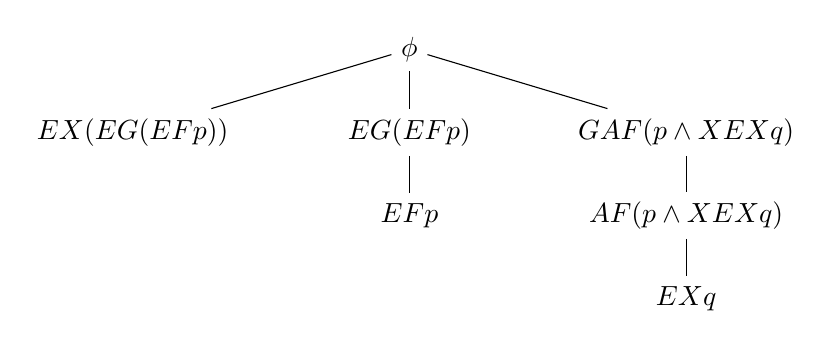
\begin{tikzpicture}[sibling distance=10em, level distance=3em]
    \node {\(\phi\)}
      child { node {\(EX(EG(EFp))\)}}
      child { node {\(EG(EFp)\)}
        child { node {\(EFp\)}}
      }
    child { node {\(GAF(p\land XEXq)\)}
      child { node {\(AF(p\land XEXq)\)}
            child { node {\(EXq\)}}
          }
        };
  \end{tikzpicture}
\end{center}

  Possiamo quindi fare questo flattening aggiungendo le atomi proposition.

\begin{center}
  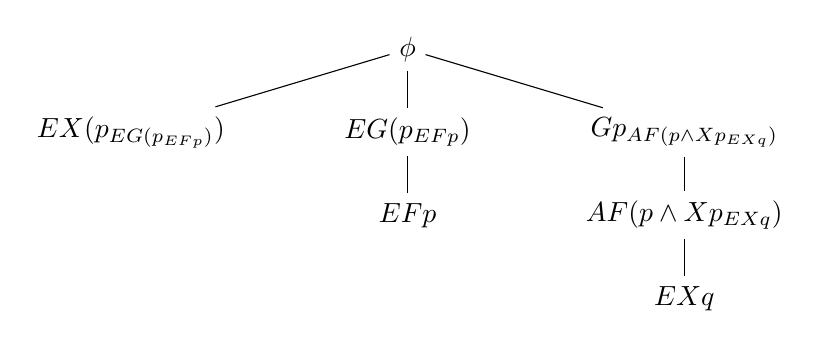
\begin{tikzpicture}[sibling distance=10em, level distance=3em]
    \node {\(\phi\)}
      child { node {\(EX(p_{EG(p_{EFp})})\)}}
      child { node {\(EG(p_{EFp})\)}
        child { node {\(EFp\)}}
      }
    child { node {\(Gp_{AF(p\land Xp_{EXq})}\)}
      child { node {\(AF(p\land Xp_{EXq})\)}
            child { node {\(EXq\)}}
          }
        };
  \end{tikzpicture}
\end{center}

Chiaramente la complessità di questo algoritmo è n volte quella di LTL, che è PSPACE\@, con \(n\) numero di sottoformule di \(CTL^*\), che è lineare nella lunghezza della formula, dunque complessità totale è ancora PSPACE\@.

Un altro modo è di usare automi ad albero, che riesce a ottenere PSPACE\@. Per quato riguarda SAT e VALIDITY, è possibile mostrare che si arriva 2EXPTIME a differenza di LTL che rimane PSPACE\@.

\(CTL^*\) però è un gran guadagno a livello di espressività. Infatti LTL è contenuto in \(CTL^*\) poiché ogni formula \(\psi\) in LTL è equivalente a \(A \psi\) in \(CTL^*\). Inoltre è stato anche dimostrato che si può verificare anche il contrario in un certo senso, ovvero data una formula \(\phi \in CTL^*\) se esista un \(\psi \in LTL\) tale che \(\phi \equiv A\psi\).

È stato mostrato infatti che presa una formula in \(CTL^*\) e eliminando banalmente tutti i quantificatori si ottiene una formula in LTL che è l'unica possibile formula LTL equivalente all'originale una volta quantificata universalmente a monte. Di conseguenza presa una qualsiasi formula \(\phi \in CTL^*\) si può facilmente produrre \(\hat{\phi} \in LTL\) eliminando i quantificatori, e poi mostrare che \(\phi \equiv A \hat{\phi}\) che è verificabile riducendo il problema a SAT della formula \(\neg ((\phi \to A \hat{\phi}) \land (A\hat{\phi} \to \phi)) \). Se questa formula è soddifacibile allora le formule non sono equivalenti, altrimenti lo sono. 

Questa idea può essere estesa anche a \(CTL\), ovvero data una formula \(\phi \in CTL\) esiste una formula \(\psi \in LTL\) tale che \(\phi \equiv A\psi\). Essendo infatti \(CTL\) un frammento di \(CTL^*\) si può appllicare banalmente l'algoritmo di cui sopra.

Un'ultima domanda è l'inversa, ovvero data \(\psi \in LTL\) esiste una formula \(\phi \in CTL\) tale che \(\psi \equiv A\phi\)? A tale domanda ad oggi non è stata data una risposta, e rimane un problema aperto.

Andiamo a vedere dunque qualche esempio di formula \(CTL^*\) non esprimibile in \(CTL\)\@.
Consideriamo \(A FGp\). Prendiamo ad esempio il modello seguente.

TODO MIGLIORA 

p -> ~p -> p (entrambi i p self loop)

L'estensione ad albero di tale modello è chiaramente

                   p
                ~p   p
               p  ~p   p
             p   p   ~p p

Chiaramente qui \(A FGp\) vale. Proviamo a vedere di trasformarla in \(CTL\). La cosa più ovvia sarebbe \(A FEGp\) oppure \(A FAGp\). Putroppo non funziona. \(A FAGp\) è falsa già nel modello di esempio, mentre \(A FEGp\) è vera nel modello dato ma esistono altri modelli per cui \(A FGp\) è vera e \(A FEGp\) no, quindi non sono equivalenti. Una possibile causa del problema è la natura esistenziale di \(F\) che cozza con \(A\).

Altro esempio è \(AF(p \land Xp)\). Anche qui, la formula più ovvia è \(AF(p \land AXp)\) ma purtroppo non è vera già nel modello di esempio perché nel percorso con soli p ogni nodo ha almeno un figlio con etichetta \(\neg p\), mentre \(AF(p \land Xp)\) è vera. Se invece consideriamo \(AF (p\land EXp)\) questa è soddisfatta dal modello

~p -> p -> ~p (2 e 3 con self loop)

la cui estensione ad albero è

                   ~p
                    p
                 ~p   p
                ~p  ~p p

Ma la formula originale non è soddifatta qui, perché ci sono percorsi in cui non ci sono mai due p consecutive.

Un ultimo esempio è con la classica fairness \(A(GFp\to Fq)\). Anche qui, la formula più ovvia è \(AG AF p \to AFq\) ma qui si vede subito che il quantificatore iniziale ha cambiato scope. In particolare in modelli che falsificherebbero l'originale possono soddisfare la seconda falsificando la premessa dell'implicazione.

Vediamo ora un esempio di proprietà \(CTL\) non esprimibile in \(LTL\). Consideriamo \(AGEFp \in CTL\). Vogliamo mostrare che non esiste \(\psi \in LTL\) tale che \(AGEFp \equiv A\psi\). Supponiamo per assurdo che esista tale \(\psi\).
Consideriamo quindi il modello k

s0 -> s1 -> s3 (self)
      ||
      s2 (self)

Se s3 è etichettata con \(p\) si ha sempre vero \(EFp\) perché s3 è sempre raggiungibile. Di conseguenza tale modello soddisfa \(AG EFp\).

Consideriamo allora il modello k' senza s3, ovvero

s0 -> s1
      ||
      s2 (self)

Qui non è mai soddisfatta p quindi non può essere soddisfatta \(EFp\) e dunque non è soddisfatta \(AG EFp\).
Ma possiamo notare che tutti i percorsi infiniti di questo secondo modello appartengono anche al primo.
Quindi essendo che \(k\models AGEFp\) allora \(k \models A\psi\) e quindi in particolare \(k\models \psi\). Ma essendo che tutti i percorsi di k' sono in k, ed essendo che le formule LTL lavorano su i percorsi abbiamo \(k' \models \psi\) e quindi \(k' \models A\psi\) e quindi \(k' \models AGEFp\), che è assurdo.

Chiudiamo con un diagramma di Venn che esemplifica la gerarchia di espressività dei linguaggi visti

TODO aggiungi diagramma 
\(CTL^*\) contiene entrambi che hanno intersezione non vuota ma non sono contenuti
A p U q è intersezione
AGEF p solo in CTL
\(AF(p \land Xp)\) solo in LTL
la loro congiunzione è solo in \(CTL^*\)

Inizio logica giochi.

\chapter{Lezione 13/05}

Per rappresentare efficientemente le tabelle di verità (funzioni booleane) passeremo per alberi di decisione, da cui potremo poi passare a grafi eliminando rindondanza arrivando ai BDD, ovvero Binary Decision Diagram, che sono dei DAG\@.

Questa rappresentazione è fortemente legata alla forma normale ITF (if-then-else). Per questa forma normale serve introdurre un operatore booleano ternario della forma generale \(\phi \to \phi_1,\phi_2\) che intuitivamente rappresenta una formula che assume il valore di verità di \(\phi_1\) se \(\phi\) è vera e il valore di verità di \(\phi_2\) se \(\phi\) è falsa. Di conseguenza è equivalente a \((\phi \land \phi_1) \lor (\neg \phi \land \phi_2)\). A questo punto, la connessione con gli alberi di decisione è immediata, poiché se \(\phi\) è una variabile proposizionale, otteniamo l'operatore \(x\to \phi_1,\phi_2\) che si mappa nativamente in nodi di un albero di decisione con \(x\) che etichetta il nodo e \(\phi_1,\phi_2\) saranno i sottoalberi figli. A questo punto con anche \(\phi_1,\phi_2\) in forma normale ITF, possiamo ottenere un albero di decisione completo. Di conseguenza ogni albero di decisione può essere riformulata in una formula che usa solo l'operatore ternario appena visto, usando i simboli costanti \(1,0\) per rappresentare vero e falso.

Dunque questo operatore può esprimere anche \(\land,\lor, \neg\). Ad esempio \(x \land y\) è equivalente a \(x \to y,0\), \(x \lor y\) è equivalente a \(x \to 1,y\) e \(\neg x\) è equivalente a \(x \to 0,1\).

Anche se l'operatore è definito sulle formule, si può mostrare per induzione che ci si può ridurre sempre ad applicare l'operatore if-then-else a variabili proposizionali. I casi base infatti sono \(0\) e \(1\) che sono già in forma normale ITF\@, e \(x\) che è esprimibile come \(x\to 1,0\). Passando al caso induttivo, consideriamo la formula \(\phi_1 \to \phi_2,\phi_3\). Essendo che \(\phi_1\) è sottoformula, per ipotesi induttiva dev'esserci una \(x\) tale che \(\phi_1 = x \to \psi_1,\psi_2\). A questo punto, possiamo riscrivere \(\phi_1 \to \phi_2,\phi_3\) come \((x \to \psi_1,\psi_2) \to \phi_2,\phi_3\). Con una semplice analisi per casi possiamo vedere che questa formula equivale a \(x\to(\psi_1\to\phi_2,\phi_3),(\psi_2\to\phi_2,\phi_3)\), da cui abbiamo la tesi. Possiamo notare come questa nuova struttura sia molto più simile ad un albero di decisione, interpretando le formule come (sotto)-alberi, e le variabili come nodi.

Data una funzione \(f\) sulle variabili booleane \(x_1,\dots,x_n\) possiamo definire il concetto di \keyword{cofattore positivo/negativo} rispetto a \(x_i\), ovvero \(f_{x_i = 1}(x_1, \ldots, x_{i-1}, 1, x_{i+1}, \ldots, x_n)\) e \(f_{x_i = 0}(x_1, \ldots, x_{i-1}, 0, x_{i+1}, \ldots, x_n)\). Shannon notò che ogni funzione booleana \(f\) che contiene una variabile \(x\) è rappresentabile come \((x\land f_x) \lor (\neg x \land f_{\overline{x}})\), con \(f_x\) e \(f_{\overline{x}}\) rispettivamente cofattori positivo e negativo di \(f\) rispsetto a \(x\). Chiaramente tale forma è analoga alla forma normale ITF.

Passando ai BDD, questi sono dei DAG a radici finite con 1 nodo iniziale (senza archi entranti), 2 nodi terminali (senza archi uscenti e etichettati con 0,1) e tutti i nodi non terminali hanno esattamente (2 archi uscenti) chiamati arco basso (0) e arco alto (1).

Ogni sequenza di bit corrisponde a un percorso in questo grafo dal nodo iniziale a nodi terminali. Questo ci permette di ridurre la ridondanza della rappresentazione dell'albero di decisione.

Vediamo come identificare queste ridondanze e di ridurre gli alberi a BDD. Le idee sono
\begin{itemize}
  \item Condividere i nodi terminali uguali
  \item Rimuovere test ridondanti, ovvero nodi che hanno due figli uguali (che sono stati uniti da altre regole) possono essere sostituiti col proprio figlio
  \item Condividere i nodi non terminali uguali, ovvero se si hannno sottodiagrammi radicati in due nodi isomorfi è possibile preservarne uno solo rimpiazzando gli archi entranti in quello rimosso con archi entranti in quello preservato.
\end{itemize}

Aggiungere esempi grafici dalle slide.

Il test di isomorfismo può sembrare complesso perché sembrerebbe che bisogni guardare l'intero sotto diagrammi, ma se le regole si applicano dal basso verso l'altro, il test di isomorfismo diventa locale, ovvero due nodi sono radice di sottodiagrammi isomorfi sono se hanno la stessa etichetta e hanno arco basso e arco alto che vanno rispettivamente negli stessi nodi. Questo è perché se i figli di un nodo erano isomorfi saranno già stati compattati da applicazioni precedenti della regola.

Tale rappresentazione purtroppo non è ancora canonica, perché per la stessa funzione è possibile scegliere una qualsiasi variabile per etichettare il nodo iniziale, ottenendo BDD completamente diversi. Di conseguenza in linea di principio ogni ordinamento sui test porta a un grafo diverso. Dunque per la forma canonica sarà ottenuta fissando un ordinamento sulle variabili.
A questo punto è possibile definire gli OBDD, ovvero ordered BDD, ovvero dei BDD in cui tutte le variabili compaiono nell'ordinamento e se \(i<j\) allora \(x_i\) appare prima di \(x_j\) in ogni percorso dal nodo iniziale a nodi terminali. In questo modo, con l'ordinamento fisso, è possibile mostrare che per ogni funzione booleana esiste un unico OBDD\@.

Questo ci sarà molto utile perché vorrà dire che il test di uguaglianza tra insiemi possiamo ridurlo a un test di isomorfismo tra OBDD (che essendo canonici sono unici) che può essere fatto in tempo lineare sulle dimensioni dell'OBDD\@. In realtà l'eliminazoine della ridondanza è applicabile all'intera foresta di BDD per tutte le possibili funzioni, ammettendo più radici per creare un unico BDD che rappresenta tutte le funzioni. In questo modo due funzioni equivalenti faranno riferimento allo stesso ogetto, e di conseguenza la verifica di isomorfismo diventa costante, ovvero il test che l'ogetto relativo alle due funzioni abbia lo stesso identificativo (puntatore).

L'ordine non è importante solo per la canonicità, ma anche per la dimensione del diagramma finale. Consideriamo infatti la funzione \(f(x_1,x_2,y_1,y_2) = 1 \iff x_1 = y_1 \land x_2 = y_2\). Se l'ordinamento è \(x_1,y_1,x_2,y_2\) allora il BDD avrà dimensione \(3 \cdots 2 +2  = 8\). In generale se la formula è \(\bigwedge_{i=1}^n x_i = y_i\) e l'ordinamento è \(x_1,y_1,x_2,y_2,\dots,x_n,y_n\) allora il BDD avrà dimensione \(3 \cdots n +2\) e quindi cresce linearmente. Se invece l'ordinamento fosse \(x_1,x_2,\ldots, x_n,y_i,y_2, \ldots y_n\) la dimensione sarà \(3\cdot 2^n-1\) e quindi esponenziale.

Aggiungere esempi grafici per mostrare perché vale questa cosa. da slide.

Sfortunatamente funzioni diverse hanno ordinamenti ottimali diversi. Inoltre decidere qual'è l'ordinamento ottimale è un problema NP-completo.

Nella pratica vengono adottate euristiche, ma non c'è garanzia di ordinamenti che mantengono l'insieme dei nodi compatti.
Per la costruzione di questi ROBDD (reduced OBDD) sarà sufficiente il seguete algoritmo

AGGIUNGI DA SLIDE.

Questi algoritmi garantiscsono che l'OBDD non contenga ridondanze.

\chapter{Lezione 18/05}

Parliamo di logica per strategia e concurrent game structure. Abbiamo visto l'esempio di sasso carta forbice. Ora vedremo la formalizzazione di struttura di giochi cercando di capire il perché le cose sono importanti e poi vedremo una logica per parlare di questi giochi ovvero ATL che è un ESTENZIONE di CTL\@.

\begin{definition}{Concurrent Game Structure}
  Una \keyword{concurrent game structure} è una quadrupla \(G=\langle AP, Ag, Ac,Ps, p_0 \in Ps, \delta, \lambda \rangle\) con
\begin{itemize}
  \item \(AP\) insieme di atomic proposition
  \item \(Ag\) insieme di agenti o giocatori
  \item \(Ac\) insieme di azioni che gli agenti possono compiere\footnote{In realtà è possibile anche avere un insieme di azioni per ogni agente, ma per semplicità consideriamo un unico insieme di azioni condiviso da tutti gli agenti}
  \item \(Ps\) insieme delle posizioni del gioco, analogo ai mondi o gli stati di una struttura di kripke
  \item \(p_0\) posizione iniziale
  \item \(\delta\) funzione di transizione
  \item \(\lambda: Ps \to 2^{AP}\) funzione di etichettatura
\end{itemize}

\end{definition}

Come possiamo notare, questa è molto vicina a una kripke structure che è definita come \(K=\langle AP,W,w_0 \in W,R,\lambda\rangle\) con \(AP\) insieme di atomic proposition, \(W\) insieme di stati, \(w_0 \in W\) stato iniziale, \(R \subseteq W\times W\) relazione di transizione seriale, ovvero tale che \(\forall w\exists v (w,v) \in R\), e \(\lambda: W \to 2^{AP}\) funzione di etichettatura.

La differenza principale è che \(\delta\) non è una relazione ma una funzione, perché modella l'evoluzione a valle delle azioni degli agenti. In particolare stando modellando giochi concorrenti e non a turni. Di consiguenza avremo \(\delta: Ps \times Ac^{Ag} \to Ps\) dove \(Ac^{Ag}\) è l'insieme delle funzioni che associano a ogni agente un azione. Questo insieme è quello che modella il non determinismo, poiché a differenza delle kripke structure questo è catturato dalle azioni dei giocatori.

Proviamo quindi a modellare sasso-carta-forbici. Sicuramente avremo
\begin{itemize}
  \item \(Ag = \set{1,2}\)
  \item \(Ac = \set{S,C,F}\)
  \item \(Ps = \set{p_0, p_1, p_2}\) con \(p_0\) stato iniziale in cui non c'è un vincitore, \(p_1\) stato in cui vince il giocatore 1 e \(p_2\) stato in cui vince il giocatore 2.
  \item \(p_0 = p_0\)
\end{itemize}

Le transizioni sono espresse dall'automa seguente:

AGGIUNGI AUTOMA
che è formalizzato da \(\delta\) che è definita come segue
\[\delta(p,(a_1,a_2)) = \begin{cases}
                          p_0 & \text{se } a_1 = a_2 \land p = p_0 \\
                          p_1 & \text{se } (a_1,a_2) \in \set{(S,F),(C,S),(F,C)} \land p = p_0 \\
                          p_2 & \text{se } (a_1,a_2) \in \set{(S,C),(C,F),(F,S)} \land p = p_0 \\
                          p & \text{se } p \in \set{p_1,p_2}
                        \end{cases}\]

\begin{note}
  Nonostante abbiamo formalizzato \(\delta\) come una funzione che chiede una funzione che associa agenti a azioni, rappresentando gli agenti con numeri è possibile esprimere la funzione come una tupla in cui a ogni posizione è assocciato l'agente con lo stesso numero che rappresenta l'agente che compie quell'azione. Ad esempio, \(\delta(p,(S,C))\) è equivalente a \(\delta(p, d)\) con \(d(1) = S\) e \(d(2) = C\). Tali funzioni sono dette \keyword{decisioni collettive}.
\end{note}

Questo poiché stiamo modellando sasso-carta-forbice come un gioco che si gioca una sola volta, e dunque una volta che si è arrivati in uno stato di vittoria non si esce più da quello stato.

Per quanto riguarda \(AP\) e \(\lambda\) come solito dipende dalle proprietà che vogliamo verificare. Ad esempio con \(AP = \set{{win}_1, {win}_2}\) che indicano rispettivamente se il giocatore 1 o 2 ha vinto, e con \(\lambda(p_0) = \emptyset\), \(\lambda(p_1) = \set{{win}_1}\) e \(\lambda(p_2) = \set{{win}_2}\) possiamo verificare proprietà riguardo la vittoria.

Con questo modello oltre che a giochi è possibile modellare in generale qualsiasi tipo di interazioni tra agenti che interagiscono concorrentemente nel modificare un sistema, come ad esempio processi che interagiscono in un sistema distribuito, o robot che interagiscono in un ambiente condiviso, o anche persone che interagiscono in un sistema sociale.

Inoltre, questa modellizzazione è sufficientemente generale da poter modellare anche giochi non concorrenti, ma a turni. Vediamo ad esempio il tris.

AGGIUNGI ESEMPIO INIZIALE DEL GRAFO DEGLI STATI DEL TRIS (già presente nella cartella images)

con i numeri vicino agli stati che indicano quante altre posizioni simmetricamente equivalenti ci sono.

Chiaramente qui avremo \(Ag = \set{\times, \circ}\). Dobbiamo capire come codificare le varie caselle, che in questo caso descrivono anche le azioni essendo che ogni giocatore come azione può solo riempire col proprio simbolo una casella. Possiamo ad esempio codificare le caselle con i numeri da \(1\) a \(9\). Dovremmo anche capire come codificare le azioni non permesse, che potremo modellare con una sconfitta automatica.

Venendo quindi agli stati, enumerarli tutti è molto comlicato avendo \(9\) celle con \(3\) possibili valori diversi, ovvero vuota \(\square\), \(\times\) e \(\circ\). Dunque il modo migliore per descriverlo è \(\set{\square, \times, \circ}^9\), ovvero le posizioni sono descritte da funzioni che associano a ogni cella cosa c'è dentro. Dovremmo anche aggiungere due stati per indicare una mossa errata, ovvero \(\set{\bot_{\times}, \bot_{\circ}}\) A questo punto avremo lo stato inziale rappresentato dalla funzione che associa \(\square\) a tutte le celle, ovvero \(p_o: n \to \square, \forall n \in \set{1,\dots,9}\).

Ora il vero momento in cui codifichiamo il fatto che il gioco è a turni, ovvero la funzione di transizione. In particolare dovremmo semplicemente ignorare l'azione del giocatore di cui non è il turno.
Ad esempio come prima mossa potremmo avere
\[\delta(p_0, d) = \set{p_i: *\setminus i \mapsto \square, i \mapsto \times}[ i = d(1)]\]

o ad esempio per la posizione \(5\)

\[\delta(p_5, d) = \begin{cases}
  p_{5i}: * \setminus \set{5,i} \mapsto \square, 5 \mapsto \times, i \mapsto \circ & ,d(2) = i \\
\end{cases}\]

Questo modello ci viene utile rispetto alle strutture di kripke, poiché tali strutture modellano tutto ciò che non è il sistema come un unica entità inglobata dal non determinismo. Questo tipo di struttura ci fornisce più granularità, potendo modellare ogni entità che interagisce nel sistema in modo autonomo e quinid carattarizzare comportamenti antagonisti, colaborativi o un mix delle due.

Ci serve adesso un linguaggio per parlare di proprietà di questo sistema, e quindi andremo a introdurre una logica estensione di CTL e \(CTL^*\).

Vedremo la logica \(ATL\) e \(ATL^*\), ovvero Alternating-time temporal logic.

Queste logiche si basano su macchine alternati, ovvero a differenza delle macchine non deterministiche che richiedono l'esistenza di run accettanti, o delle macchine universali che richiedono che ogni run accetti, qui si dovrà avere un alternanza di esistenzialità e universalità.

\begin{definition}{\(ATL^*\)}
  \[\phi := p \mid \neg \phi \mid \phi \land \phi \mid \phi \lor \phi \mid \GDia[A]\psi \mid \GBox[A] \psi\]
  \[\psi := \phi \mid \neg \psi \mid \psi \land \psi \mid \psi \lor \psi \mid X\psi \mid \psi U\psi \mid \psi R \psi\]

  Con \(A \subseteq Ag\). Intuitivamente si ha
  \begin{itemize}
    \item \(\GDia[A] \psi\) è vera se esiste una strategia \(\sigma^+\) per i giocatori di \(A\) tale che, per ogni strategia \(\sigma^-\) di \(Ag\setminus A\) tale che \(\pi\models \psi\) con \(\pi\) è il percorso identificato dalla coppia \(\sigma^+, \sigma^-\)
    \item \(\GBox[A] \psi\) è vera se per ogni strategia \(\sigma^+\) per i giocatori di \(A\) esiste una strategia \(\sigma^-\) di \(Ag\setminus A\) tale che \(\pi\models \psi\) con \(\pi\) è il percorso identificato dalla coppia \(\sigma^+, \sigma^-\)
  \end{itemize}

  In un certo senso \(\GDia \psi\) è una generalizzazione di \(E\psi\) e \(\GBox \psi\) è una generalizzazione di \(A\psi\) per giochi a un giocatore, dove \(Ag = A = \set{1}\) e \(Ag\setminus A = \emptyset\).
\end{definition}

\begin{definition}{\(ATL^*\)}
  \[\phi := p \mid \neg \phi \mid \phi \land \phi \mid \phi \lor \phi \mid \GDia[A]\psi \mid \GBox[A] \psi\]
  \[\psi := \phi \mid X\psi \mid \psi U\psi \mid \psi R \psi\]


\end{definition}

Tali definizioni sono ancora informali, ma possiamo già notare che questi operatori son duali, nel senso che \(\neg \GDia[A]\psi \equiv \GBox[A] \neg \psi\)

Dobbiamo andare quindi a formalizzare il concetto di strategia e di percorso in una concurrent game structure.

Partendo da percorso, avremo che \(\pi \in Path(G) \subseteq Ps^\omega\) se \(\forall i \in [0,\abs{\pi}-1). \exists d \in Ac^{Ag}. \pi_{i+1} = \delta(\pi_i,d)\). Il che è equivalente a vedere i percorsi nella struttura di kripke sottostante. Alcuni percorsi però possono dipendere dalla sotria delle decisioni prese dai giocatori.

Questo in realtà è un problema che c'era anche nelle strutture di kripke e nelle logiche temporali. Prendiamo ad esempio la struttura

AGGIUNGI FOTO GIAÀ PRESENTE NELLA CARTELLA IMAGES

Chiaramente questa struttura verifica \(F(p\land Fq)\). Ma per farlo è necessario fare scelte diverse in \(w_0\), e quindi devo ricordarmi delle scelte passate per fare quelle giuste. Se facessi scelte guardado solo lo stato attuale non sarei in grado di soddisfarle. In reltà si dimostra che se non ci fosse memoria potrei verificare solo percorsi lasso, ovvero con la forma:

AGGIUNGI IMMAGINE

Si dimostra però che per avere proprietà per cui è indispensabile la memoria mi serve innestare operatori temporali, e quindi rimanendo in CTL o in ATL la memoria non sarà necessaria.

A questo punto però è necessario anche il concetto di storia:

\[Hst = \set{\pi \in Path(G)}[\abs{\pi} < \omega]\]

Possiamo quindi definire una strategia come
\[\sigma: Hst \to Ac\]

Ovvero una funzione che associa a ogni posizione della storia una azione, intuitivamente quella che è stata presa nella posizione.
Ovviamente una trategia per un insieme di giocatori \(A\subseteq Ag\) sarà \(\set{\sigma_a}_{a \in A}\), ovvero una sequenza di strategie per ogni giovatore.

Una coppia di strategie di gruppi di giocatori tali che l'unione dei gruppi è \(Ag\) è detta \(play\):
\[\pi = play(\sigma_A,\sigma_{Ag\setminus A}) \in Path(G,p_0)\]
tale che \(\pi\) è coerente con le scelte fatte dai giocatori nelle strategie \(\sigma_A\) e \(\sigma_{Ag\setminus A}\), ovvero

\[\forall i \in \N, \pi_{i+1} = \delta(\pi_i, d_i)\]
con
\[d_i(a) = \begin{cases}
  \sigma_A^a(\pi_{\leq i}) & a \in A \\
  \sigma_{Ag\setminus A}^a(\pi_{\leq i}) & a \in Ag\setminus A
\end{cases}\]

Ovvero a ogni passo \(i\) la posizione successiva è determinata dalle azioni scelte dai giocatori in quel passo, che sono determinate dalle strategie che dipendono dalla storia fino a quel punto.

Noi ci concentreremo essenzialmente su ATL poiché ha la proprietà di poter essere soddisfatta da strategie memoryless, ovvero in cui una strategia è esclusivamente \(\sigma: Ps\to Ac\) ovvero solo l'ultimo stato conta. Non vedremo la dimostrazione, ma idealmente si può mostrare che se una formula è soddisfatta da percorsi con cicli non semplici posso sempre eliminare i cicli non semplici accorpandoli in un unico ciclo semplice che mi crea la struttura a lasso.

Essendo che le strategie memoryless di fatto identificano degli archi avremo che un play identifica un sottografo, in cui mantengo solo gli archi effettivamente percorsi. Tra l'altro tale grafo è deterministico, ovvero partendo dallo stato inziale esiste un solo percorso.

A questo punto per verificare prorietà sarà sufficiente verificare la raggiungibilità su i vari sottografi indotti.

Essendo che gli operatori \(\GDia\) e \(\GBox\) nascondono internamente una quantificazione alternata (\(\forall\exists, \exists\forall\)) non è possibile in CTL esprimere tutto ciò che è esprimibile in ATL. In particolare CTL è semanticamente un frammento di ATL in cui scelgo solo coalizioni \(A=\emptyset\) o \(A = Ag\) rendendo vacuo un quantificatore.

Inoltre abbiamo visto che in CTL erano vere proprietà di one-step unfolding, ovvero

\[A/E \phi_1 U \phi_2 \equiv \phi_2 \lor (A/E \phi_1 \land A/E X(A/E \phi_1 U \phi_2))\]
\[A/E \phi_1 R \phi_2 \equiv \phi_2 \land (A/E \phi_1 \lor A/E X(A/E \phi_1 R \phi_2))\]

Inoltre osservando che queste proprietà è di punto fisso abbiamo potuto riscriverla come \(E \phi_1 U \phi_2 \equiv \mu V. \phi_2 \lor (\phi_1 \land EX V)\) e \(E \phi_1 R \phi_2 \equiv \nu V. \phi_2 \land (\phi_1 \lor EX V)\) da cui abbiamo estratto gli algoritmi di model checking. Anche in ATL sono presenti delle equazioni di punto fisso identiche. Di conseguenza l'unica cosa che dovremo cambiare per il model checking sarà solo l'operatore pre, che sarà più complicato dovendo cogliere l'alternanza.

\chapter{Lezione 20/05}

L'ultima volta ci siamo fermati a una possibile implementazione di OBDD che è molto vicina a quella che effettivamente si fa, in particolare si usano due tabelle, una che rappresentano un grafo e un altra per fare hashing delle triple per ottenere i nomi dei nodi, in modo da garantire l'unicità.

Ora dobbiamo vedere come implementare le operazioni su questi OBDD, ovvero le operazioni insiemistiche (\(\cap, \cup, \overline{S}\)) e la preimmagine \(pre(P) = \den{EXP} = \set{s}[s\to t \land t \in \den{P} \text{ per qualche }t]\) che serve sia per \(EX\) che per iterarla nei punti fissi per \(EU\) e \(EG\). Quindi dati gli OBDD di due funzioni booleane \(f\) e \(g\) vorremmo calcolare l'OBDD per \(f \circ g\) con \(\circ \in \set{\cap, \cup, \overline{S}}\). Ricordiamo che avendo fissato un ordine sulle variabili abbiamo rappresentato le funzioni \(f\) come \((x_1 \land f_{x_1}) \lor (x_2 \land f_{\overline{x_1}})\). Se vogliamo quindi \(\cup\), ovvero \(\lor\) tra le funzioni abbiamo: 


\begin{equation*}
  f \lor g = \begin{aligned}
    ((x_1 \land f_{x_1}) \lor (\neg x_1 \land f_{\overline{x_1}})) \lor ((x_1 \land g_{x_1}) \lor (\neg x_1 \land g_{\overline{x_1}})) = \\
    x_1 \land (f_{x_1} \lor g_{x_1}) \lor \neg x_1 \land (f_{\overline{x_1}} \lor g_{\overline{x_1}})
    \end{aligned}
\end{equation*}

Questo vale anche per \(\land\) e \(\neg\). 

TODO: FAI I CONTI A CASA 

Essendo che \(\neg f \equiv f \oplus 1\) possiamo esprimere tutti gli operatori con un unico algoritmo che è identico se non nei casi base.

VEDI ALGORITMO DA SLIDE.

Nota che nei casi in cui uno dei BDD dipende da una variabile da cui l'altro non dipende non fa entrambe le chiamate ricorsive ma solo quello che dipende perché tanto l'altro è invariato.

Questo algoritmo di pase ha complessità \(\BigO(2^n)\) perché ripeto più volte le stesse chiamate ricorsive, ma posso risolvere con programmazione dinamica, ovvero mantenendo una cache o tabella dei risultati parziali già calcolati, in modo che per ogni tripla \(op,u,v\) la chiamata ricorsiva venga fatta una volta sola, mentre negli altri casi si andrà a vedere a tempo costante la look-up table. Fissato \(op\) è chiaro che quindi le chiamate saranno esattamente \(\BigO(\abs{f}\cdot \abs{g})\) e quindi la complessità totale sarà \(\BigO(\abs{f}\cdot \abs{g})\).

Ora prendiamo ad esempio una funzione \(f(x_1,\ldots,x_n)\) e di voler calcolare i cofattori rispetto a una certa \(x_i\), ovvero calcolare la riduzione rispetto \(x_i\), denotata come \(f(x_1,\ldots,x_n)_{|_{x_i}}\) o \(f(x_1,\ldots,x_n)_{|_{\overline{x_i}}}\) che corrispondono rispettivamente a \(f(x_1,\ldots,x_{i-1}, 1, x_{i+1},\ldots,x_n)\) e \(f(x_1,\ldots,x_{i-1}, 0, x_{i+1},\ldots,x_n)\). Questo induce un altra possibile operazione sugli OBDD ovvero l'operazione di restrizione rispetto a un assegnamento, ovvero dato un OBDD \(f\) e un assegnamento \(\sigma\) a una parte delle variabili contenute in \(f\) di creare l'OBDD della riduzione di \(f\) rispetto alle variabili di \(\sigma\). Possiamo notare come anche in questo caso usando l'espansione di shannon nel caso in cui la variabile discriminante non sia nell'assegnamento, possiamo spingere l'operazione sui sottoalberi, mentre se è presente è sufficiente scegliere il ramo corrispondente all'assegnamento.

Questo è in particolarmodo utile per le Quantified Bolean formulae, ovvero formule booleane quantificate, con semantica identica al prim'ordine su dominio booleano.

Da un punto di vista funzionale \(\exists x_i:f(x_1, \ldots, x_n)\) è la funzione booleana che valuta a \(1\) se \(f(x_1, \ldots,x_n)\) valuta a \(1\) per qualche valore di \(x_i\). È quindi equivalente a \(f_{x_i} \lor f_{\overline{x_i}}\). Dualmente per \(\forall x, f(x_1, \ldots, x_n)\) sarà \(f_{x_i} \land f_{\overline{x_i}}\). A noi servirà in particolare \(\exists\) per la preimmagine, perché è intrinsecamente una proprietà esistenziale. In caso però di logica alternante, come nei giochi, la preimmagine può essere universale.

[Discussione interessante sui collegamenti con SAT e VALIDITY e di come questo porti ad avere tempo di costruzione di OBDD esponenziale alle volte indipendentemente dall'ordinamento sulle variabili scelte.]

Finalmente capiamo come risolvere il model checking usando OBDD. Ovviamente qui si parte da strutture di kripke in input, quindi dobbiamo capire come codificarla tramite OBDD, ovvero rappresentare la topologia del grafo sottostante mediante OBDD.

Ora per insieme degli stati \(S\) basterà avere \(\lceil\log_2 \abs{S}\rceil\) variabili booleane in modo che ogni elemento dell'insieme sarà codificato in un numero in binario, e l'appartenenza sarà identificata tramite la funzione caratteristica, che da \(1\) se e solo se l'elemento appartiene a \(S\). Senza perdità di generalità possiamo assumere che se due stati hanno la stessa etichetta sono lo stesso stato. Di conseguenza sarà possibile costruire le funzioni caratteristiche per i singleton delle proposizioni atomiche e metterle in disgiunzione. In particolare per la variabile atomica \(p\) per rappresentare lo stato in cui è vera solo \(p_1\) basterà usare la formula \(p_1 \bigwedge_{i \neq 1} \neg P_i\) per ogni \(i\). Per la relazione invece abbiamo chiaramente \(R\subseteq S\times S\). Avendo già la rappresentazione degli stati tramite \(x_1, \ldots, x_{\log_2\abs{S}}\) variabili, mi è sufficiente raddoppiare le variabili ottenendo \(x_1', \ldots, x_{\log_2\abs{S}}'\) e avere un OBDD che dipenda da entrambe le sequenze di variabili, in modo che le prime rappresentano il primo elemento della coppia e il secondo la seconda.

AGGIUNGI ESEMPI!

A questo punto per l'ordine conviene mettere consecutive variabili e la loro primata, essendo strettamente correlate.

Possiamo quindi costruire l'algoritmo tramite OBDD\@.

Facciamo induttivamente:
APPROFONDIRE DA SLIDE
\[\den{x_i} = f_{x_i}(x_1, \ldots, x_{n}) = x_i\]

Per gli operatori booleani basterà fare l'operatore booleano tra le funzioni delle sottoformule

Ci manca la preimmagine, ovvero \(EX\phi\). In prima battuta mi serve l'insieme degli archi che terminano in \(\den{\phi}\). Ma per fare questo mi basta prendere \(f_{\phi}(x_1,\ldots,x_n)\) e trasformarlo in \(f_{\phi}(x_1', \ldots, x_n')\) in modo da interpretarlo come stati di arrivo, e poi fare l'intersezione con \(f_{R}\). Questo perché di fatto ogni OBDD può essere visto come su tutte le variabili, primate e non, semplicemente non dipenderà da quelle che non gli riguardano.

Ora chiaramente a me serve ricavare solo gli archi di partenza quindi posso astrarre esistenzialmente con \(\exists x_1', \ldots,x_n'\). Quindi in generale \(\den{EX\phi}= \exists x_1',\ldots,x_n': (f_{\phi}(x_1,\ldots,x_n)\land f_{R}(x_1,x_1',\ldots,x_n,x_n'))\).\footnote{Si può fare anche in maniera molto più efficiente applicando la quantificazione esistenziale eagerly, ovvero spingendo la quantificazione esistenziale più in basso possibile, ovvero al primo momento in cui la variabile quantificata compare, in modo da ridurre la grandezza degli OBDD intermedi.}

A questo punto per \(EU\) e \(EG\) basterà applicare gli algoritmi classici di punto fisso.

È facile vedere che \(\abs{f_S}\leq 2^n\) con \(n\) numero di variabili, quindi \(\abs{f_S}\leq 2^{\log_2 \abs{S}} = \abs{S}\). Quindi la complessità è alla peggio uguale dell'algoritmo tramite etichettatura, ma in una buona parte dei casi la grandezza è meno che esponenziale, e quindi ci saranno tanti casi in cui si farà meglio.

\chapter{Lezione 25/05}

La struttura di kripe indotta da una concurrent game structure è essenzialmente la stessa con \(R\) tale che \((s_1,s_2) \in R\) se e solo se \(\exists d \in Ac^{Ag}. s_2 = \delta(s_1,d)\). Questo giustifica il vedere ATL come estensione di CTL e in particolare vedere gli operatori \(\GDia\) e \(\GBox\) come generalizzazioni di \(E\) e \(A\). Nella terminologia dei giochi l'insieme di agenti vengono dette coalizioni. Quindi \(\GDia[A] \psi\) ci diche che esiste una stategia per la coalizione \(A\) tale che ogni strategia della coalizione complementare \(\overline{A}\) verificano \(\psi\) e dualmente per \(\GBox\).

Abbiamo quindi formalizzato il concetto di strategia analizzando il fatto che tali strategie dipendono dalla storia. Noi ci concentreremo solo sulle strategie memoryless.

Possiamo definire quindi in modo più preciso la semantica degli operatori \(\GDia\) e \(\GBox\) in ATL\@.

\[G,s\models \GDia[A] \psi \text{ se } \exists \sigma_A \in Str(A) \forall \sigma_{\overline{A}} \in Str(\overline{A}). G,s,play(\sigma_A,\sigma_{\overline{A}})\models \psi \]

Si vede facilmente che l'unica differenza rispetto a CTL è la quantificazione sulle strategie degli avversari. Se infatti consideriamo \(\GDia[Ag] \psi\) allora \(\overline{A} = \emptyset\) e quindi \(\GDia[Ag] \psi\equiv E\psi\). Il verso \(\implies\) è banale, mentre per quello inverso basta prendere il percorso che soddisfa \(E\psi\) e costruire per ogni passo la strategia adeguata, non essendoci una coalizione antagonista.

\[G,s\models \GBox[A] \psi \text{ se } \forall \sigma_A \in Str(A) \exists \sigma_{\overline{A}} \in Str(\overline{A}). G,s,play(\sigma_A,\sigma_{\overline{A}})\models \psi \]

Ovvviamente si ha \(\GBox[Ag] \psi \equiv A\psi\) con dimostrazione simile a quella precedente. Quindi CTL equivale a ATL con la \keyword{grand coalition}, ovvero una coalizione di tutti gli agenti. Dunque ATL è più espressiva.

Prendendo l'esempio di carta sasso forbice possiamo dire che esistono weak strategy, ovvero per ogni agente c'è una strategia dell'altro che lo avvantaggia. Formalmente
\[\GBox[\set{1}] F s_1\land \GBox[\set{2}] F s_2\]
Ma non ci sono strategie vincenti
\[\neg \GDia[\set{1}] F s_1 \land \neg \GDia[\set{2}] F s_2\]

ATL non ha bisogno di memoria, nel senso che le proprietà che richiedono memoria non sono esprimibili in ATL.

Per fare l'algoritmo di Model checing CTL abbiamo sfruttato il one-step unfolding che ci ha permesso di costruire una funzione monotona e quindi sfruttare una costruzione a punto fisso. Cerchiamo di farlo anche per ATL.

In particolare abbiamo visto
\[E \phi_1 U\phi_2 \equiv \phi_2 \lor (\phi_1\land E X E \phi_1 U\phi_2)\]

Dobbiamo mostrare che valga
\[\GDia[A] \phi_1 U\phi_2 \equiv \phi_2 \lor (\phi_1\land \GDia[A] X \GDia[A] \phi_1 U\phi_2)\]

È facile vedere che \(\GDia[A] \phi_1 U\phi_2 \equiv \phi_2 \lor (\phi_1\land \GDia[A] X \phi_1 U\phi_2)\) perché è sufficiente prendere la strategia che rende vera la formula che assumo vera e usarla per l'altra e si vede facilmente che va bene pure per l'altra. La parte difficile è nello spezzare gli operatori temporali. In CTL quando spezzavamo un percorso era facile perché il next non era altro che prendere il primo e poi il resto. Adesso abbiamo un alternanza di quantificatori in principio e quindi la scelta di una strategia scelta aprioristicamente che mi assicura \(U\) per quanto riguarda \(GDia[A] X \phi_1 U\phi_2\). Nello spezzare in \(\GDia[A] X \GDia[A] \phi_1 U\phi_2\) invece mette su una doppia alternanza perché la semantica è

\[\exists \sigma_A \forall \sigma_{\overline{A}} \exists \sigma_{A}' \forall \sigma_{\overline{A}}' play(\sigma_{A}',\sigma_{\overline{A}}',{\left(play(\sigma_A,\sigma_{\overline{A}},s)\right)}_1) \]

Quello che vorremmo mostrare è che questa alternanza è irrilevante, e che bastano i primi due quantificatori. Una perima versione per i giochi a somma zero finiti il cui goal è un istanza di reachability è stato dimostrato da Zermelo che è sempre vero che almeno un giocatore ha una strategia vincente.

\[\exists \sigma_1 \forall \sigma_2 Win_1(\sigma_1,\sigma_2) \lor \exists \sigma_2 \forall \sigma_1 Win_2(\sigma_1,\sigma_2) \]

Nel prim'ordine questa struttura è falsificabile da un qualsiasi modello a grafo che non ha ne oggetti iniziali ne terminali. Ma per i giochi finiti a somma zero questo è sempre verificato. Questo in oltre vale solo per i giochi a turni.

Un modo per mostrare quindi che si può spezzare creando un gioco a somma zero tra un verificatore e un rifiutatore della formula e sfruttare il teorema di zermelo per mostrare che almeno uno dei due ha una strategia vincente. 

Un altro modo è costruttivo, usando le strategie della formula che assumo vera per costruire quelle della formula che voglio mostrare equivalente. Se ad esempio vogliamo mostrare \(\GDia[A] X \phi_1 U\phi_2 \implies \GDia[A] X \GDia[A] \phi_1 U\phi_2\) posso usare la strategia del primo per copiarla per la seconda, e mostrare che va bene. Nell'altro verso invece ne ho due, allora uso quella del next per fare il per togliere il primo stato dalla history e poi quella dell'until appropriato rispetto al risultato della strategia del next per il resto. Si passa quindi da strategie senza memoria a temporaneamente strategia con memoria che posso sempre riportare a memoria zero.

Funziona uguale per il release:

\[\GDia[A] \phi_1 R \phi_2 \equiv \phi_2 \land (\phi_1 \lor \GDia[A] X \GDia[A] \phi_1 R\phi_2)\]

A differenza di CTL non potremo passare al \(G\) perché questa formula non distribuisce
\[\GDia[A] \phi_1 R \phi_2 \equiv \GDia[A] ((\phi_2 U (\phi_2 \land \phi_2)) \lor G \phi_2)\]

In ogni caso però con la stessa identica dimostrazione vista per CTL questi sono ancora rispettivamente minimo e massimo punto fisso. L'unica differenza è che dovremo fare induzione completa su un albero di percorsi piuttosto che induzione lineare su un singolo percorso.

Quindi quello che ci rimane è l'operatore \(X\) o equivalentemente nella forma denotazionale la funzione \(pre\). Questa è la grande sostanziale differenza, poiché avendo più giocatori il concetto di preimmagine è più complesso. Prima infatti \(pre\) catturava \(EX\), ma ora dobbiamo fare \(\GDia[A]X\). Nella semantica dovremmo lavorare sulle strategie, ma essendo che stiamo lavorando con \(X\) ci interessa solo un passo, e quindi ci interessa delle due strategie solo l'azione dato lo stato di partenza. Quindi
\[\exists \sigma_A \forall \sigma_{\overline{A}} play(\sigma_A,\sigma_{\overline{A}},s) \models X\phi \]
diventa
\[\exists {ac}_{A} \forall {ac}_{\overline{A}} \delta(s, ({ac}_A, {ac}_{\overline{A}})) \models \phi\]

Ora la definizone matematica di \(pre\) era
\[pre(V) = \set{w\in W}[\exists w' \in V. (w,w') \in R]\]

Ora però c'è un universale da trattare quindi dovremo aggioranare a 
\[pre_A(V) = \set{w\in W}[\exists {ac}_{A} \in Ac^A \forall {ac}_{\overline{A}} \in Ac^{\overline{A}}. \delta(w, ({ac}_A, {ac}_{\overline{A}})) \in V]\]

Essendo che a livello algoritmico l'unica cosa usata di fatto è il punto fisso (che rimane uguale) e il \(pre\) ci basta per il model checking cambiare il \(pre\) di CTL con questa versione più a grana fine.

Questo algoritmo rimane polinomiale sugli archi, ma purtroppo questo algoritmo è esponenziale nei giocatori, poiché per ogni stato e ogni azione della coalizione \(A\) devo verificare tutte le azioni della coalizione complementare \(\overline{A}\). In generale però se il numero di giocatori è piccolo, o se le azioni sono limitate, questo algoritmo è comunque efficiente.

\chapter{Lezione 27/05}

Riprendiamo il modello di automi temporizzati usati per modellare sistemi che lavorano a tempo reale. Quello che vorremmo fare è il verificare proprietà temporali su questi sistemi. Una prima proprietà semplice è REACHABILITY, ovvero verificare, dato in input un TA e uno stato di controllo, se dagli stati iniziali esista almeno un percorso fino allo stato obiettivo. Ogni stato abbiamo detto essere una coppia \((l,\nu)\) con \(l\in Loc\) e \(\nu: C \to \R\). Formalmente quindi il problema di reachability è: dato un TA \(A\) e uno stato di controllo \(l_f \in Loc\) esiste un run divergente tale che esiste un indice \(i\) per cui \(\pi = s_0 s_1 \ldots s_i \ldots\) con \(s_0 \in Loc_0\) e \(s_i = (l_f, \nu)\) per qualche \(\nu\)?

Tale problema è decicibile finquando ci interessa solo la locazione. Se invece volessimo raggiungere uno stato specifico, ovvero una specifica coppia \((l_f,\nu_f)\) in input non è più decidibile.

In ogni caso essendo il numero di stati infinito lo spazio di ricerca è infinito la raggiungibilità non è banale. Tipicamente l'esplorazione di uno spazio infinito è decidibile se lo spazio può essere partizionato in un numero finito di classi di equivalenza rilevanti per il problema d'interessse, ovvero tali che ogni elemento all'interno di una classe è equivalente per il problema considerato. Ad esempio per la raggiungibilità potrebbero essere le componenti fortemente connesse, che però sono potenzialmente infinite a loro volta.

POTENZIALMENTE AGGIUNGERE IMMAGINE ESEMPIO

Quello che ci serve è una proprietà più forte, perché ci serve una sorta di proprietà di similuazione, nel senso che ogni stato in una classe di equivalenza deve poter fare tutto ciò che fanno gli altri a livello di classi. Se uno stato in una classe \(C_1\) può andare in uno stato in \(C_2\) vorrei che ogni altro elemento di \(C_1\) vada in qualche modo in \(C_2\). Ovviamente essendo le locazioni finite la cosa importante è definire un'equivalenza tra le valutazioni \(\nu\). Tali classi di equivalenza sono dette \keyword{Regioni}. In un TA chiaramente i comportamenti sono determinati dalle invarianti e dai vincoli sui clock, i quali sono ovviamente finiti. Per la definizione della classe di equivalenza consideriamo i seguenti criteri:

\begin{itemize} 
  \item Due valutazioni di clock sono equivalenti se e solo se soddisfano gi stessi vincoli di clock
  \item Due valutazioni equivalenti devono dar luogo a run simili
  \item Devono esserci un numero finito di classi
\end{itemize}

Andiamo ad analizzare i vincoli di clock. Consideriamo \(x ~ c\) con \(c \in \N\) e \(~ \in \set{<,> =,\leq,\geq}\).
Allora per \(x<c\), \(\nu(x)\models c\) se e solo se \(\nu(x)< c\) o, essendo intero, \(\lfloor \nu(x) \rfloor < c\). Per quelli di ugualianza possiamo contare la parte frazionaria, controllando che siano uguali le parti frazionarie. Quindi se ci fossero solo vincoli interi. Abbiamo però considerato vincoli nei razionali, ma possiamo sempre ricondurci agli interi moltiplicando per il minimo comune multiplo dei denominatori. 

Consideriamo lo spazio euclideo in ficura che rappresenta lo spazio di tutte le valutazioni sui clock \(x\) e \(y\).

AGGIUNGI IMMAGINE DA SLIDE!

La regione in grigio sono proprio tutte le valutazioni equivalenti tra loro rispetto al vincolo indicato.

Quindi l'equivalenza sta partizionando lo spazio continuo in riquadri interni aperti, che rappresentano i vincoli con sole disequazioni strette, i punti di intersezioni, unici intervalli chiusi, che rappresentano vincoli con solo relazioni di uguagianza e segmenti, sempre aperti topologicamente, che rappresentano vincoli con un uguaglianza e una disugualgianza. Quindi per un numero arbitrario di clock la partizione diventa su ipercubi. Questa prima decopoosizione rispetta il primo vincolo ma non sappiamo ancora se rispetta il generare run simili. Consideriamo i path più semplici dove passa solo il tempo, no transizione discrete, otteniamo quello che abbiamo ad immagine

AGGIUNGI FOTO

Come possiamo vedere punti della stessa classe vanno in classi diverse.

Possiamo notare però che l'unica differenza è sulla parte frazionaria. In particolare possiamo notare che queste due valutazioni danno luogo a stati che hanno potenziali futuri diversi. Quello che è sufficiente però è tagliare i rettangoli usando la diagolane, che corrisponde ad avere la parte frazionaria uguale.

Quindi per la partizione oltre a vedere il valore intero della valutazione e se il valore frazionario è zero o meno, ma anche se l'ordine delle parti frazionarie di tutti i clock sia uguale per tutte le valutazioni. Ovviamente la diagonale in se sarà una classe di equivalenza a sé stante, ovvero dove le parti frazionarie sono tutte uguali.

Abbiamo quindi un partizionamento di questo tipo

IMMAGINE TRIANGOLI

Purtroppo però abbiamo ancora un numero infinito di classi di equivalenza. È però possibile risolvere facilmente questa cosa guardando la massima costante di confronto per ogni variabile, chiaramente tutte le classi che sono definite dall'avere quel clock maggiore della massima costante sono equivalenti perché l'automa non può distinguere tra quelle classi

IMMAGINE TRIANGOLI E RIQUADRO ILLIMITATO x>3 y >3

In particolare quelle in cui entrambi clock sforano la massima costante non sono più distinguibili, mentre quelle in cui solo uno sfora sono ancora distinguibili da altre ma non internamente perché non dipendono più dall'altro clock. Con quindi i clock \(x\) e \(y\) e massime costanti \(c_y\) e \(c_x\) abbiamo un primo partizionamento a triangolo come visto per la sottoregione \(x\leq c_x \land y \leq c_y\), una classe per ogni valore intero minore di \(y\) che assorbono tra loro tutti i casi \(x> c_x \land y \leq c_y\), ugualie per \(x\) e una classe unica per entrambi i clock sopra le rispettive costanti.

Il conto complessivo delle regioni si dimostra che non supera
\[\abs{C}! \cdot 2^{\abs{C}-1}\Pi_{x \in C} (2c_x+2)\]
 con \(c_x\) massima costante presente nel TA in un vincolo per \(x\). Intuitivamente ogni regione può essere identificata da una tripla \(\langle I, \pi, D\rangle\) dove
\begin{itemize}
  \item \(I\) una famiglia di intervalli, con per ogni \(x \in C\) un  \(I_x \in \set{[0,0], ]0,1[, [1,1], ]1,2[\ldots,]c_x-1,c_x[,[c_x,c_x]}\)
  \item \(\pi\) una permutazione dei clock che rappresenta l'ordine sulle parti frazionarie. Ovviamente \(\abs{\pi} = \abs{C}\).
  \item \(D\subset C\) che ci indica tra quali clock della permutazione vale l'uguaglianza. In particolare se \(x\in D\) varrà l'uguaglianza tra \(x\) è il predecessore nell'ordinamento. Chiaramente \(\abs{D}\leq\abs{C}-1\).
\end{itemize}

Possiamo quindi vedere che il numero di permutazioni di \(C\) elementi è proprio \(\abs{C}\)!, il numero di sottinsiemi di un insieme di cardinalità \(\abs{C}-1\) è \(2^{\abs{C}-1}\) mentre il numero di intervalli che si forma è proprio la produttoria che abbimo visto nel calcolo, poiché per ogni clock \(x\) con costante massima \(c_x\) avremo che ogni \(n \in \N\) con \(n\leq c_x\) appare in esattamente due intervalli. Essendoci quindi \(c_x +1\) elementi avremo \(2c_x +2\) intervalli per clock.

Avendo partizionato lo spazio delle valutazioni posso partizionare in modo finito lo spazio degli stati considerando come equivaleni stati con la stessa locazione e valutazioni equivalenti che rappresenterò con la regione. A questo punto dobbiamo andare a costruire l'automa definendo la relaizone di transizione. In particolare avrà la transizione \((l,R)\to(l',R')\) se per ogni \(\nu \in R\) esiste un \(\nu' \in R'\) tale che esista nel grafo originario \((l,\nu)\to (l,\nu')\).

Dobbiamo quindi capire come si comporano le transizioni di reset. In particolare andiao a definire delle regioni di reset per ogni regione. Chiaramente questa dal punto di vista geometrico equivale a una proiezione sull'asse corrispondente al clock resettato. Chiaramente per più reset basta applicare più proiezioni di seguito. Questo ci permette di modellare facilmente le transizioni discrete.

AMPLIA IL CONCETTO

Definiamo invece le regioni successore di una regione come la prima regione che raggiungo facendo esclusivamente passare il tempo.
Questo ci permette di definire le transizione di time-elapse.

Possiamo quindi definire l'automa delle regioni come 

\[RTS =\langle S,\Sigma\cup\set{\tau}, \to', Init, AP', L'\rangle\]

Dove:

\begin{itemize}
  \item \(S = \set{\langle l,r\rangle}[l \in Loc, r \text{ regione}]\)
  \item \(Init = \set{\langle l_0, r\rangle}[l_0 \in Loc_0, r \text{ regione con tutti i clock a } 0]\)
  \item \(AP' = AP\cup \Phi(C)\) 
  \item \(L'(\langle l,r\rangle) = L(l)\cup \set{\phi \in \Phi(C)}[r \models \phi]\)
  \item \(\langle l,r\rangle \xrightarrow{\omega} \langle l',r'\rangle\) se \(l \xrightarrow{a,\lambda,r} l'\) con \(a = \omega\)
\end{itemize}

Chiaramente questo partizionamento giustifica il perché possiamo risolvere problemi di raggiungibilità solo se non pretendiamo una specifica valutazione, poiché l'informazione su di esse scompare nell'automa delle regioni. Possiamo comunque decidere raggiungibilità tra regioni, ovvero se è possibile raggiungere una qualsiasi valutazione che appartiene a una certa regione target.

Inoltre è possibile definire anche un estensione delle logiche branching come CTL ad automi temporizzati con Timed CTL, definita come segue
\[\phi ::= True\mid p \in AP\mid g \in \Phi(C)\mid \neg \phi\mid \phi_1\land\phi_2\mid \phi_1\lor\phi_2\mid E \phi_1 U_I \phi_2 \mid E G_I \phi\]
dove \(I\) sono intervalli di tempo in cui dev'essere presente il testimone dell'\(U\) o del \(G\).

La semantica di \(E \phi U_I \psi\) intuitivamente è che dev'esserci un \(\psi \in I\) e fino a che non lo raggiungo dev'esser vero \(\phi\). Formalmente 
\(s\models E \phi_1 U_I \phi_2\) se esiste un percorso divergente \(\pi\in Paths_{div}(d)\) con \(\pi = s_0 \xrightarrows{d_0} s_1 \xrightarrows{d_1} s_2 \ldots\) con \(s_0 = s\) e
\begin{itemize}
  \item \(\sum_{j=0}^{i-1} (d_j )+ d \in I\) per qualche \(i\) tale che \(d \in [0,d_i]\) e \(s+d\models \phi_2\)
  \item \(\forall j\leq i, s_j+d' \models \phi_1\lor \phi_2\) per ogni \(d' \in [0,d_j]\) con \(\sum_{k=0}^{j-1} d_k+d' \leq \sum_{k=0}^{i-1} d_k + d\)
\end{itemize}

Per fare model checking sarà sufficiente trasformare ogni intervallo presente in una formula \(U\) o \(F\) in una guardia su un nuovo clock per poi trasformare in CTL standard.

GUARDA SLIDE PER DETTAGLI

\whitepage{}
\makebackcover{}

\end{document}